% Options for packages loaded elsewhere
\PassOptionsToPackage{unicode}{hyperref}
\PassOptionsToPackage{hyphens}{url}
%
\documentclass[
]{book}
\usepackage{lmodern}
\usepackage{amsmath}
\usepackage{ifxetex,ifluatex}
\ifnum 0\ifxetex 1\fi\ifluatex 1\fi=0 % if pdftex
  \usepackage[T1]{fontenc}
  \usepackage[utf8]{inputenc}
  \usepackage{textcomp} % provide euro and other symbols
  \usepackage{amssymb}
\else % if luatex or xetex
  \usepackage{unicode-math}
  \defaultfontfeatures{Scale=MatchLowercase}
  \defaultfontfeatures[\rmfamily]{Ligatures=TeX,Scale=1}
\fi
% Use upquote if available, for straight quotes in verbatim environments
\IfFileExists{upquote.sty}{\usepackage{upquote}}{}
\IfFileExists{microtype.sty}{% use microtype if available
  \usepackage[]{microtype}
  \UseMicrotypeSet[protrusion]{basicmath} % disable protrusion for tt fonts
}{}
\makeatletter
\@ifundefined{KOMAClassName}{% if non-KOMA class
  \IfFileExists{parskip.sty}{%
    \usepackage{parskip}
  }{% else
    \setlength{\parindent}{0pt}
    \setlength{\parskip}{6pt plus 2pt minus 1pt}}
}{% if KOMA class
  \KOMAoptions{parskip=half}}
\makeatother
\usepackage{xcolor}
\IfFileExists{xurl.sty}{\usepackage{xurl}}{} % add URL line breaks if available
\IfFileExists{bookmark.sty}{\usepackage{bookmark}}{\usepackage{hyperref}}
\hypersetup{
  pdftitle={R Kompendium für die kommunikationswissenschaftliche Statistik- und Datenanalyse-Ausbildung am IJK Hannover},
  pdfauthor={Julia Niemann-Lenz},
  hidelinks,
  pdfcreator={LaTeX via pandoc}}
\urlstyle{same} % disable monospaced font for URLs
\usepackage{color}
\usepackage{fancyvrb}
\newcommand{\VerbBar}{|}
\newcommand{\VERB}{\Verb[commandchars=\\\{\}]}
\DefineVerbatimEnvironment{Highlighting}{Verbatim}{commandchars=\\\{\}}
% Add ',fontsize=\small' for more characters per line
\usepackage{framed}
\definecolor{shadecolor}{RGB}{248,248,248}
\newenvironment{Shaded}{\begin{snugshade}}{\end{snugshade}}
\newcommand{\AlertTok}[1]{\textcolor[rgb]{0.94,0.16,0.16}{#1}}
\newcommand{\AnnotationTok}[1]{\textcolor[rgb]{0.56,0.35,0.01}{\textbf{\textit{#1}}}}
\newcommand{\AttributeTok}[1]{\textcolor[rgb]{0.77,0.63,0.00}{#1}}
\newcommand{\BaseNTok}[1]{\textcolor[rgb]{0.00,0.00,0.81}{#1}}
\newcommand{\BuiltInTok}[1]{#1}
\newcommand{\CharTok}[1]{\textcolor[rgb]{0.31,0.60,0.02}{#1}}
\newcommand{\CommentTok}[1]{\textcolor[rgb]{0.56,0.35,0.01}{\textit{#1}}}
\newcommand{\CommentVarTok}[1]{\textcolor[rgb]{0.56,0.35,0.01}{\textbf{\textit{#1}}}}
\newcommand{\ConstantTok}[1]{\textcolor[rgb]{0.00,0.00,0.00}{#1}}
\newcommand{\ControlFlowTok}[1]{\textcolor[rgb]{0.13,0.29,0.53}{\textbf{#1}}}
\newcommand{\DataTypeTok}[1]{\textcolor[rgb]{0.13,0.29,0.53}{#1}}
\newcommand{\DecValTok}[1]{\textcolor[rgb]{0.00,0.00,0.81}{#1}}
\newcommand{\DocumentationTok}[1]{\textcolor[rgb]{0.56,0.35,0.01}{\textbf{\textit{#1}}}}
\newcommand{\ErrorTok}[1]{\textcolor[rgb]{0.64,0.00,0.00}{\textbf{#1}}}
\newcommand{\ExtensionTok}[1]{#1}
\newcommand{\FloatTok}[1]{\textcolor[rgb]{0.00,0.00,0.81}{#1}}
\newcommand{\FunctionTok}[1]{\textcolor[rgb]{0.00,0.00,0.00}{#1}}
\newcommand{\ImportTok}[1]{#1}
\newcommand{\InformationTok}[1]{\textcolor[rgb]{0.56,0.35,0.01}{\textbf{\textit{#1}}}}
\newcommand{\KeywordTok}[1]{\textcolor[rgb]{0.13,0.29,0.53}{\textbf{#1}}}
\newcommand{\NormalTok}[1]{#1}
\newcommand{\OperatorTok}[1]{\textcolor[rgb]{0.81,0.36,0.00}{\textbf{#1}}}
\newcommand{\OtherTok}[1]{\textcolor[rgb]{0.56,0.35,0.01}{#1}}
\newcommand{\PreprocessorTok}[1]{\textcolor[rgb]{0.56,0.35,0.01}{\textit{#1}}}
\newcommand{\RegionMarkerTok}[1]{#1}
\newcommand{\SpecialCharTok}[1]{\textcolor[rgb]{0.00,0.00,0.00}{#1}}
\newcommand{\SpecialStringTok}[1]{\textcolor[rgb]{0.31,0.60,0.02}{#1}}
\newcommand{\StringTok}[1]{\textcolor[rgb]{0.31,0.60,0.02}{#1}}
\newcommand{\VariableTok}[1]{\textcolor[rgb]{0.00,0.00,0.00}{#1}}
\newcommand{\VerbatimStringTok}[1]{\textcolor[rgb]{0.31,0.60,0.02}{#1}}
\newcommand{\WarningTok}[1]{\textcolor[rgb]{0.56,0.35,0.01}{\textbf{\textit{#1}}}}
\usepackage{longtable,booktabs}
\usepackage{calc} % for calculating minipage widths
% Correct order of tables after \paragraph or \subparagraph
\usepackage{etoolbox}
\makeatletter
\patchcmd\longtable{\par}{\if@noskipsec\mbox{}\fi\par}{}{}
\makeatother
% Allow footnotes in longtable head/foot
\IfFileExists{footnotehyper.sty}{\usepackage{footnotehyper}}{\usepackage{footnote}}
\makesavenoteenv{longtable}
\usepackage{graphicx}
\makeatletter
\def\maxwidth{\ifdim\Gin@nat@width>\linewidth\linewidth\else\Gin@nat@width\fi}
\def\maxheight{\ifdim\Gin@nat@height>\textheight\textheight\else\Gin@nat@height\fi}
\makeatother
% Scale images if necessary, so that they will not overflow the page
% margins by default, and it is still possible to overwrite the defaults
% using explicit options in \includegraphics[width, height, ...]{}
\setkeys{Gin}{width=\maxwidth,height=\maxheight,keepaspectratio}
% Set default figure placement to htbp
\makeatletter
\def\fps@figure{htbp}
\makeatother
\setlength{\emergencystretch}{3em} % prevent overfull lines
\providecommand{\tightlist}{%
  \setlength{\itemsep}{0pt}\setlength{\parskip}{0pt}}
\setcounter{secnumdepth}{5}
\usepackage{booktabs}
\usepackage{amsthm}
\makeatletter
\def\thm@space@setup{%
  \thm@preskip=8pt plus 2pt minus 4pt
  \thm@postskip=\thm@preskip
}
\makeatother
\usepackage{titling}
\usepackage{icomma}
\ifluatex
  \usepackage{selnolig}  % disable illegal ligatures
\fi
\usepackage[]{natbib}
\bibliographystyle{apalike}

\title{R Kompendium für die kommunikationswissenschaftliche Statistik- und Datenanalyse-Ausbildung am IJK Hannover}
\author{Julia Niemann-Lenz}
\date{2021-09-09}

\begin{document}
\maketitle

{
\setcounter{tocdepth}{1}
\tableofcontents
}
\begin{Shaded}
\begin{Highlighting}[]
\FunctionTok{options}\NormalTok{(}\AttributeTok{OutDec=} \StringTok{","}\NormalTok{)}
\end{Highlighting}
\end{Shaded}

\hypertarget{herzlich-willkommen}{%
\chapter*{Herzlich Willkommen!}\label{herzlich-willkommen}}
\addcontentsline{toc}{chapter}{Herzlich Willkommen!}

Mit diesem Lehrbuch möchte ich Ihnen in die Programmiersprache R näher bringen. Es ist zum einen als begleitendes Lernmaterial für die Statistikausbildung am \emph{Institut für Journalistik \& Kommunikationswissenschaft der Hochschule für Musik, Theater \& Medien Hannover} gedacht. Zum anderen soll es als Nachschlagewerk dienen. Aus diesen Gründen ist es nicht einem bestimmten Kurs zugeordnet, sondern enthält eine Sammlung von Erklärungen, Anleitungen und Skripten. Das Buch richtet sich sowohl an Einstieger:innen, die gerade mit der Statistik-Grundausbildung beginnen, als auch an Umsteiger:innen, die bisher mit einem anderen Statistikprogramm (vermutlich mit SPSS) gearbeitet haben.

R hat in den letzten Jahren innerhalb der Kommunikationswissenschaft stark an Bedeutung gewonnen, da es den Erfordernissen moderner Datenanalyse sehr viel besser entgegenkommt als herkömmliche Statistiksoftware. Denn die Anforderungen haben sich geändert: Durch die Digitalisierung und die damit einhergehende Datafizierung sind heute mehr Daten verfügbar den je und auch die Struktur der Daten hat sich gewandelt. Beispielsweise rückt die automatisierte Analyse von Textdaten zunehmend in den Fokus und Kommunikationsdaten aus Social Media weisen eine Netzwerkstruktur auf.

Digitale Daten sind ein bedeutender Wirtschaftsfaktor, der oft höher eingeschätzt wird als manifeste Güter. Vielfach handelt es sich bei den nun verfügbaren Daten um Kommunikationsdaten. Deshalb sind Expert:innen, die sowohl fundiertes Domänenwissen im Bereich Kommunikation und Medien, als auch die Kompetenz Daten fachgerecht auszuwerten mitbringen, in der Kommunikationspraxis sehr gefragt. Aber auch in den Sozialwissenschaften führt der ``Computational Turn'' zu deutlichen Veränderungen. Die Subdisziplin ``Computational Communication Science'' ist mittlerweile längst kein Trend mehr, sondern eine feste Größe der Forschungslandschaft. Verfahren aus dem Bereich der Informatik und der Statistik erweitern das traditionelle Methodenspektrum. Sie werden auch als ``Compuational Methods'' bezeichnet. Angesichts der ``Reproduktionskrise'' sind zudem die Anforderungen an die Transparenz und Reproduzierbarkeit von wissenschaftlichen Erkenntnissen gestiegen. Während die bisher eingesetzte proprietäre Statistiksoftware die neuen Anforderungen nicht oder nur unzureichend erfüllen kann, kommen Programmiersprachen diesen Bedarfen flexibel entgegen.

\hypertarget{dank}{%
\section*{Dank}\label{dank}}
\addcontentsline{toc}{section}{Dank}

Ich bedanke mich beim Bundespresseamt für die Erlaubnis den hier benutzten Datensatz zum Zweck dieses Lehrbuchs verwenden zu dürfen.

Quellenangabe:

Presse- und Informationsamt der Bundesregierung (2020). Generation Z. GESIS Datenarchiv, Köln. ZA6738 Datenfile Version 1.0.0 (2020), \href{https://dbk.gesis.org/dbksearch/sdesc2.asp?no=6738\&db=e\&doi=10.4232/1.13446}{doi:10.4232/1.13446}.

\hypertarget{disclaimer}{%
\section*{Disclaimer}\label{disclaimer}}
\addcontentsline{toc}{section}{Disclaimer}

Das Buch Work in Progress! Ich habe im Wintersemester 2020 mit dem Aufbau des Kompeniums begonnen. Es ist ein ganz besonderes Semester, das zweite unter Corona-Bedingungen und diese Tatsache rückt noch einmal sehr in den Vordergrund, wie wichtig gute digitale Lernressourcen sind.

Ich bemühe mich um eine sinnhafte Gliederung, sprechende Überschriften und einen linearen Aufbau. Gerade letzteres wird jedoch an einigen Stellen kaum möglich sein. Insbesondere, wenn Sie vielleicht zu den etwas fortgeschritteneren Anwender:innen gehören, scheuen Sie sich nicht, Inhalte zu überspringen und querzulesen!

Die Erweiterung des Buches erfolgt schrittweise. Über Vorschläge für neue Inhalte, Hinweise auf Fehler und Anregungen, wie man diese Lernressource noch besser gestalten kann, freue ich mich!

\hypertarget{intro}{%
\chapter{Einleitung}\label{intro}}

In diesem Einführungs-Kapitel gebe ich einen Überblick über das R-Universum und führe in die Hintergründe und Philosophie der Sprache ein. Dabei kommen auch die vielen Vorzüge, die der Umstieg auf R für Kommunikationswissenschaftler:innen hat, zur Sprache und es werden Alternativen angesprochen.

\hypertarget{einfuxfchrung-in-r}{%
\section{Einführung in R}\label{einfuxfchrung-in-r}}

R ist eine Programmiersprache mit einem speziellen Fokus auf die Anwendung im Bereich Statistik und Data-Science. In diesem Abschnitt werde ich kurz die Hintergründe und die Entstehungsgeschichte von R erläutern.

Die simpelste Antwort auf die Frage ``Was ist eigentlich R?'' lautet: ``R ist ein Dialekt von S.'' \citep{Peng_2020}
Diese Antwort ist natürlich nicht sehr befriedigend und führt direkt zur Anschlussfrage
``Und was ist S?'' Tatsächlich ist es interessant, die Entstehungsgeschichte von S und R zu kennen und etwas übr die zugrundeliegende Philosophie der Sprachen zu erfahren.
Dadurch wird deutlich, worin die Unterschiede zu anderen Programmiersprachen liegen, warum
R von Informatikern und Programmierern häufig als ``etwas seltsam'' empfunden wird und weshalb R gerade
für die Datenanalyse in der Kommunikationswissenschaft besonders gut geeignet ist.
Deshalb hole ich an dieser Stelle etwas weiter aus.

\hypertarget{s-ist-die-mutter-von-r}{%
\subsection{S ist die Mutter von R}\label{s-ist-die-mutter-von-r}}

Die Programmiersprache S hat ihre Wurzeln in den 1970er Jahren und wurde von John Chambers,
Allan R. Wilks und Kollegen als internes Tool in den ``Bell Telephone Laboratories'' entwickelt.
Die Bell Labs waren damals Teil der Telefongesellschaft AT\&T und ein bedeutendes Forschungszentrum.
Forscher der Bel Labs haben beispielsweise mehrere Nobelpreise und Turing-Awards gewonnen.
Heute gehören die Bell Labs zu Nokia.

Mitte der 1960er Jahre war die Rechentechnik so weit, dass die Bel Labs gemeinsam mit anderen
Forschungseinrichtungen an einem Projekt zur Schaffung eines Mehrprozess- und Mehrbenutzerbetriebssystems arbeiteten (``Multics System'', Vorläufersystem von Unix).
Die Möglichkeit, dadurch auf Großrechnern Datenanalyse-Forschung ausführen zu können, war aus Sicht der Bel Laboratories sehr relevant und obwohl sie sich später nicht mehr an der Schaffung des Multics-Systems beteiligten, setzten sie die Entwicklung einer Statistiksprache fort. Diese Sprache nannten sie S - vermutlich für \emph{statistic}.
Zu dieser Zeit war die Idee einer Programmiersprache für Statistik völlig neu.
Für statistische Berechnungen war es bisher nötig, den Code direkt in FORTRAN (steht für FORmula TRANslation, das war die damals dazu genutzte Sprache) zu schreiben und zwar immer wieder aufs Neue, angepasst an die jeweilige Fragestellung.

Die erste Version von S wurde 1976 nur intern veröffentlicht. In den Folgejahren fanden einige
Veränderungen an der Sprache statt, z.B. wurde sie nun mit C als Basis und als objektorientierte
Programmiersprache weiterentwickelt. In den 1980er Jahren vergab AT\&T erstmals Lizenzen von S für
kommerzielle Zwecke und für Bildungseinrichtungen.
Nach der Aufteilung von AT\&T wurde S an das Unternehmen Statistical Science verkauft, welches eine kommerzielle Version von S entwickelte.
Diese Implementierung ist auch heute noch unter dem Namen \emph{S-Plus} verfügbar.
Ihre Verbreitung ist aber sehr gering.

\hypertarget{die-philosophie-von-s}{%
\subsection{Die Philosophie von S}\label{die-philosophie-von-s}}

Die neue Sprache S sollten bei der explorativen Datenanalyse und der Erstellung von Grafiken unterstützen
und dabei schneller und möglichst flexibel sein.
\citet{Chambers_2000} formuliert das Ziel von S so:

\begin{quote}
``S is a programming language and environment for all kinds of computing involving data. It has a simple goal: To turn ideas into software, quickly and faithfully''.
\end{quote}

Insbesondere die schnelle, explorative Übersetzung von Forschungsideen in Ergebnisse war wichtig, während die statistische Analyse am Beginn noch nicht so sehr im Fokus stand.

Zusätzlich zeichnet sich die Philosophie von S noch durch drei weitere Anforderungen aus, die
während der Entwicklung an die Programmiersprache gestellt wurden \citep[S. 84:5]{Chambers_2020}:

\begin{enumerate}
\def\labelenumi{\arabic{enumi}.}
\item
  \textbf{Convenience:} Der Aufruf von statistischen Routinen sollte möglichst ``kompakt'' sein. Die Anwender:innen sollten sich nicht mit den Details wie z.B. dem Datenmanagement beschäftigen müssen. Zudem sollte der Output grafische und formatierte Ausgaben enthalten.
\item
  \textbf{Completeness:} Alle Zusammenfassungen, Modellierungen und Visualisierungen die in FORTRAN möglich waren, sollten auch in S möglich sein.
\item
  \textbf{Extensibility:} Bereits damals verstanden sich die Entwickler von S als Teil einer Datenanalyse- und
  Forschungs-Community.
  Deshalb sollte die Sprache grundsätzlich erweiterbar sein. Neue Techniken und Methoden sollten stets in S integrierbar sein.
\end{enumerate}

\hypertarget{die-entwicklung-von-r}{%
\subsection{Die Entwicklung von R}\label{die-entwicklung-von-r}}

Parallel zur Entstehung von S-Plus entwickelten die Statistiker Ross Ihaka und Robert Gentleman
an der Universität Auckland R nach dem Vorbild von S. Die Bezeichnung \emph{R} nimmt zum einen Bezug auf das Vorbild und geht zum anderen auf die Vornamen der beiden Entwickler zurück.
Neben der Beseitigung einiger Mängel (z.B. bei der Speicherverwaltung) war es das Ziel der beiden Statistiker neue Verfahren schneller in die Programmiersprache implementieren zu können, ohne dabei auf das Entwicklerteam von S angewiesen zu sein.
Zudem lies sich der Quelltext gut für Lehrzwecke einsetzen.

Nachdem Ithaka und Gentleman R zunächst nur in der Wissenschafts-Community verbreiteten und dafür
positives Feedback erhielten, entschieden Sie sich 1995 zur Veröffentlichung der Sprache unter einer
\emph{General Public License} (GNU).
Das Basis-Paket von R (base R) wird seitdem von einem etwa 20-köpfigen Kernentwicklerteam um Ross Ihaka und Robert
Gentleman weiterentwickelt (\emph{R Core Team}).
Der gemeinnützige Verein \emph{R Foundation for Statistical Computing} mit Sitz in Wien verwaltet das Urheberrecht an R
und dient dem Zweck, die Verbreitung der Sprache zu fördern.
Dieses Bemühen kann als sehr erfolgreich beurteilt werden.
Trotz des eingeschränkten Anwendungsfokus ist R heute laut TIOBE-Index eine der beliebtesten Programmiersprachen überhaupt. Im Oktober 2020 belegt R Platz 9 des Rankings.

Aktuelles R-Logo:

\hypertarget{weiterfuxfchrende-links}{%
\subsection*{Weiterführende Links}\label{weiterfuxfchrende-links}}
\addcontentsline{toc}{subsection}{Weiterführende Links}

\begin{itemize}
\tightlist
\item
  \href{https://de.wikipedia.org/wiki/R_(Programmiersprache)}{Wikipedia-Artikel zu R}
\item
  \href{https://cran.r-project.org/}{CRAN (Comprehensive R Archive Network)}
\item
  \href{https://www.r-project.org/foundation/}{R Foundation}
\item
  \href{https://www.tiobe.com/tiobe-index/}{TIOBE-Ranking}
\end{itemize}

\hypertarget{vorteile-von-r}{%
\section{Vorteile von R}\label{vorteile-von-r}}

Man kann natürlich fragen, warum nun gerade R die optimale Wahl für die Statistik- und Datenanalyseausbildung in der Kommunikationswissenschaft und im Medienmanagment ist. Für R sprechen aus meiner Perspektive die folgenden zehn Gründe:

\begin{enumerate}
\def\labelenumi{\arabic{enumi}.}
\item
  \textbf{R ist einfach.} Als erste Programmiersprache ist R gerade für Personen, die das Interesse ``Datenanalyse'' verfolgen, gut geeignet.
\item
  \textbf{R skaliert.} Man kann mit R sowohl kurze Ad-Hoc Auswertungen machen, als auch sehr komplexe Programme schreiben. Der Übergang ist fließend und so kann man von Anwender:in zu Entwickler:in werden, ohne eine große Hürde überwinden zu müssen.
\item
  \textbf{R ist umfangreich, aktuell und zukunftssicher.} Durch den modularen Aufbau in Pakete ist es einfach, R um Funktionalität zu erweitern. Bereits jetzt existiert eine Vielzahl an Paketen, die den Funktionsumfang weit über den proprietärer Statistiksoftware hinaus erweitern. Eine aktive Entwicklercommunity arbeitet beständig daran, R noch umfangreicher und besser zu machen.
\item
  \textbf{R hat eine große, aktive Community.} Weil sowohl Entwickler- als auch Anwendercommunity groß und aktiv sind, gibt es sowohl online als auch in Form von Büchern jede Menge Hilfestellungen. Sollte sich eine Frage nicht durch Googeln lösen lassen, ist es gar nicht unwahrscheinlich, dass eine ins Netz gepostete Frage schnell und kompetent beantwortet wird.
\item
  \textbf{R unterstützt lösungsorientiertes Denken.} Anders als ``Point-and-click''-Software rückt R den Prozess der Datenanalyse in den Mittelpunkt und hilft dabei, ihn in kleine Teile herunterzubrechen. Das fördert die Problemlösekompetenz.
\item
  \textbf{R begleitet den gesamten Forschungsprozess} -- von der Datensammlung über die Datenspeicherung in Datenbanken, der Datenaufbereitung und -analyse bis hin zur Visualisierung und Kommunikation.
\item
  \textbf{R macht Forschung transparenter und reproduzierbar.} Durch die Arbeit in einer Programmiersprache ist man quasi gezwungen, die einzelnen Schritte schriftlich niederzulegen -- mindestens in Form von Code. Aber auch darüber hinaus bietet R viele weitere Funktionen und Tools zur Verbesserung der Nachvollziehbarkeit und für Open Science.
\item
  \textbf{R ist eine relevante Kompetenz auf dem Arbeitsmarkt.} - Das gilt auch und gerade für Sozial- und Kommunikationswissenschaftler:innen!
\item
  \textbf{R macht Spaß!} Programmieren ist eine kreative Tätigkeit, die durchaus auch Flow-Erlebnisse hervorrufen kann.
\item
  \textbf{R ist Open Source \& kostenlos für viele Plattformen verfügbar.} Dadurch wird nicht nur der persönliche Geldbeutel geschont, R trägt damit auch zur Liberalisierung von Wissen insgesamt bei und bietet die Möglichkeit, sich selbst an der Entwicklung der Software zu beteiligen.
\end{enumerate}

Trotz der vielen soeben herausgestellten Vorteile ist R natürlich kein Wundermittel und keine eierlegende Wollmilchsau. Eine Programmiersprache, die allen Ansprüchen genügt und dabei keine Einschränkungen hat, gibt es nicht. An dieser Stelle soll nicht unerwähnt bleiben, dass Anwender:innen die einen Hintergrund in der Informationswissenschaft oder bereits Erfahrungen mit anderen Programmiersprachen haben, R bisweilen als kompliziert, unübersichtlich oder langsam beurteilen. Zudem gilt R als ``unsicher'', wenn es darum geht, Webapplikationen zu bauen.

Aus Perspektive der (sozialwissenschaftlichen) Methodenlehre überwiegen dennoch die Vorzüge.
R kann ein guter Einstieg in die Welt des Programmierens sein. Obwohl sich R in einigen Punkten von anderen Programmiersprachen unterscheidet, sind viele Konzepte gleich und können übertragen werden, sodass es später leichter fällt, weitere Programmiersprachen zu lernen.

\hypertarget{alternativen-zu-r}{%
\section{Alternativen zu R}\label{alternativen-zu-r}}

Das R eine Programmiersprache ist, die sich besonders zur Datenanalyse und zur Berechnung von
Statistiken eignet, kam bereits mehrfach zur Sprache. Selbstverständlich gibt es aber auch noch
andere Software, die diesen Zweck erfüllen kann.
Einerseits gibt es eine Reihe (proprietärer) Anwendungen, die ebenfalls zur statistischen Analyse verwendet werden, wie beispielsweise SAS, Stata, MatLab oder SPSS.
Andererseits gibt es natürlich auch andere Programmiersprachen, die gut geeignet sind, um statistische
Berechnungen anzustellen.
Zu nennen sind an dieser Stelle vor allem Python und Julia.

\leavevmode\hypertarget{info_spss}{}%
\textbf{SPSS}

In der Kommunikationswissenschaft war bisher SPSS von IBM das am weitesten verbreitete Tool.
SPSS ist eine Statistiksoftware mit einer Benutzeroberfläche und man kann sich die Ausgabe von Statistiken quasi ``zusammenklicken''.
Man muss die dahinterliegende Programmiersprache, welche SPSS-Syntax heißt, dazu nicht im Detail kennen.
Allerdings nimmt die Verbreitung von SPSS in der Wissenschaft und in der Wirtschaft momentan
deutlich ab.
Gegen SPSS sprechen beispielsweise die hohen Lizenzkosten, die langsame Implementierung neuer Verfahren und die sinkende Verbreitung.

\hypertarget{weiterfuxfchrende-links-1}{%
\subsection*{Weiterführende Links}\label{weiterfuxfchrende-links-1}}
\addcontentsline{toc}{subsection}{Weiterführende Links}

\begin{itemize}
\tightlist
\item
  Vergleich Statistik-Software 1
\item
  Vergleich Statistik-Software 2
\item
  Popularität von Statistik-Software
\end{itemize}

\hypertarget{tipps-zum-r-lernen}{%
\section{Tipps zum R lernen}\label{tipps-zum-r-lernen}}

\hypertarget{der-anfang-ist-schwer}{%
\subsection{Der Anfang ist schwer}\label{der-anfang-ist-schwer}}

R unterscheidet sich deutlich von der Software, mit der Kommunikationswissenschaftler:innen bisher gearbeitet haben. Es handelt sich nicht um ein proprietäres Programm, sondern um eine Programmiersprache. Dadurch werden die Grenzen dessen, was möglich ist, immens erweitert. Da fällt der Ein- bzw. Umstieg am Anfang vielleicht erstmal schwer und sicherlich gehört beim Erlernen einer neuen Kompetenz immer auch eine \textbf{gewisse Frustrationstoleranz} dazu. Das nicht alles von Anfang an klappt, ist ganz normal. Es ist sehr wichtig, sich diesen Umstand zu verdeutlichen.

Artwork by Allison Horst

\hypertarget{nuxfctzliche-hinweise}{%
\subsection{Nützliche Hinweise}\label{nuxfctzliche-hinweise}}

\begin{itemize}
\item
  \textbf{Holen Sie sich die Hilfe, die Sie brauchen!}
  Welche Lern-Ressourcen für Sie die richtigen sind, können Sie selbst am besten entscheiden. Eine Person lernt vielleicht leichter mit einem interaktiven Kurs, eine andere mit einem Buch. Das ist Geschmackssache. Eine besonders hilfreiche Methode kann auch ``Vier Augen / ein Rechner'' sein, bei dem Sie mit eine:r Kommiliton:in gemeinsam am Computer üben.
\item
  \textbf{Lesen Sie Fehlermeldungen aufmerksam durch.}
  Falls ein Skript mal nicht wie erwartet funktioniert, liefert Ihnen die Fehlermeldung oft einen ersten Hinweis darauf, woran es liegen könnte. Das gilt meistens - aber leider nicht immer. Denn nicht alle Autoren der unterschiedlichen R-Pakete schreiben Fehlermeldungen, die auch für Einsteiger verständlich sind.
\item
  \textbf{Schauen Sie genau hin}.
  Achten Sie genau auf die Syntax: Häufige Fehler sind vergessene oder doppelte Klammern \texttt{\{{[}(){]}\}}, Anführungszeichen \texttt{"}oder Kommata \texttt{,}.
\item
  \textbf{Googeln ist eine Kompetenz und ausdrücklich erwünscht!}
  Wenn Sie bei einer Fragestellung feststecken und die Hilfe Sie auch nicht weiterbringt, versuchen Sie Ihre Fehlermeldung oder Ihre Fragestellung zu ergoogeln. Sie sind womöglich nicht der/die Erste, der/die vor diesem Problem steht.
\item
  \textbf{Beachten Sie die 15-Minuten-Regel.}
  Wenn Sie auf ein Problem stoßen, versuchen Sie 15 Minuten lang es zu lösen. Sollten Sie es bis dahin nicht geschafft haben, fragen Sie jemanden um Hilfe! Wenn Sie gerade an einem Seminar teilnehmen, können das natürlich bevorzugt Ihre Kommiliton:innen, Tutor:innen oder Dozierenden sein. Aber auch im Internet gibt es viele Foren z.B. stackoverflow.
\end{itemize}

Artwork by Allison Horst

\hypertarget{installation}{%
\chapter{Installation}\label{installation}}

R ist für viele verschiedene Betriebssysteme verfügbar, man kann es sogar auf einem Android-Smartphone installieren. RStudio gibt es für Windows, MacOS und Linux sowie in einer Variante für Server.

Auf den folgenden Seiten finden Sie Installationsanleitungen von R und RStudio für MacOS und Windows. Sie benötigen beide Programme (vgl. Kapitel \protect\hyperlink{benutzeroberfluxe4chen}{Benutzeroberflächen}).
Da die Installation auf beiden Betriebssystemen etwas unterschiedlich ist (insbesondere beim Download von R), sind die Wege in zwei Unterkapiteln beschreiben.

\hypertarget{installationsanleitung-windows}{%
\section{Installationsanleitung Windows}\label{installationsanleitung-windows}}

Wie auf den vorhergehenden Seiten beschrieben, handelt es sich bei R und RStudio um zwei unterschiedliche Dinge:

\begin{enumerate}
\def\labelenumi{\arabic{enumi}.}
\item
  R, die Programmiersprache
\item
  RStudio, die Entwicklungsumgebung
\end{enumerate}

Zur Installation müssen Sie deshalb auch \textbf{beides nacheinander} installieren.

\hypertarget{erster-schritt-r}{%
\subsection{Erster Schritt: R}\label{erster-schritt-r}}

Die aktuelle Version von R können Sie über das CRAN downloaden. Die Webadresse lautet: https://cran.r-project.org. Gleich auf der Startseite finden Sie die Links zu den jeweils aktuellen R-Versionen:

Klicken Sie auf ``Download R for Windows'' und klicken Sie im sich öffnenden Fenster auf „install R for the first time``.

Während diese Dokumentation geschrieben wurde, war die aktuellste Version 4.0.3, wie der nachfolgende Screenshot zeigt:

Nun klicken Sie auf den Download-Link für die aktuelle Version. Doppelklicken Sie anschließend die heruntergeladene Datei und folgen der Installationsanleitung. Die Einstellungsoptionen brauchen Sie dabei nicht anzupassen.

\hypertarget{zweiter-schritt-rstudio}{%
\subsection{Zweiter Schritt: RStudio}\label{zweiter-schritt-rstudio}}

RStudio, die Entwicklungsumgebung für R können Sie unter https://rstudio.com/products/rstudio/download/ herunterladen.
Wählen Sie die Version ``RStudio Desktop - Free''.

Nun werden sie weitergeleitet und klicken auf „Download RStudio for Windows``.

Nachdem der Download abgeschlossen ist, doppelklicken Sie die Datei und folgen erneut der Installationsanleitung. Nach der Installation können Sie das Programm RStudio öffnen. Es greift automatisch auf die zuvor installierte Version von R zu.

\hypertarget{installationsanleitung-macos}{%
\section{Installationsanleitung MacOS}\label{installationsanleitung-macos}}

Wie auf den vorhergehenden Seiten beschrieben, handelt es sich bei R und RStudio um zwei unterschiedliche Dinge:

\begin{enumerate}
\def\labelenumi{\arabic{enumi}.}
\item
  R, die Programmiersprache
\item
  RStudio, die Entwicklungsumgebung
\end{enumerate}

Zur Installation müssen Sie deshalb auch \textbf{beides nacheinander} installieren.

\hypertarget{erster-schritt-r-1}{%
\subsection{Erster Schritt: R}\label{erster-schritt-r-1}}

Die aktuelle Version von R können Sie über das CRAN downloaden. Die Webadresse lautet: https://cran.r-project.org. Gleich auf der Startseite finden Sie die Links zu den jeweils aktuellsten R-Versionen:

Klicken Sie auf der https://cran.r-project.org auf ``Download R for (Mac) OSX'' und scrollen Sie bis zu den ``Latest Releases''. Unter dieser Überschrift wird Ihnen die aktuellste ``stable'' Version von R angezeigt.

Während diese Dokumentation geschrieben wurde, war dies die Version 4.0.2, wie der nachfolgende Screenshot zeigt:

Rechtsklicken Sie auf die Version und laden Sie sie herunter.

Doppelklicken Sie auf die heruntergeladene Datei und folgen Sie der Installationsanleitung.

\hypertarget{zweiter-schritt-rstudio-1}{%
\subsection{Zweiter Schritt: RStudio}\label{zweiter-schritt-rstudio-1}}

RStudio, die Entwicklungsumgebung für R können Sie unter \textless a href = ``\url{https://rstudio.com/products/rstudio/download/}'' target =‚ "\_blanc"\textgreater https://rstudio.com/products/rstudio/download/ herunterladen.

Wählen Sie die Version ``RStudio Desktop - Free'' und laden Sie die Datei herunter.

Nachdem der Download abgeschlossen ist, doppelklicken Sie die Datei und ziehen Sie sie in Ihre Applications.

Nach der Installation können Sie das Programm RStudio öffnen. Es greift automatisch auf die zuvor installierte Version von R zu.

\hypertarget{benutzeroberfluxe4chen}{%
\chapter{Benutzeroberflächen}\label{benutzeroberfluxe4chen}}

In diesem Abschnitt finden Sie alles, was Sie zum Start über die Benutzeroberfläche von R und RStudio wissen müssen. Dabei gehe ich zu nächst auf die R-Konsole ein: Ein Tool, dass bereits beim Download von R mitgeliefert wird und in dem Sie die Sprache bereits ausführen können - wenngleich dies wenig komfortabel ist. Die R-Konsole ist aber auch ein Teil von RStudio. Im Anschluss gehe ich deshalb auf die IDE und ein paar ausgewählte Features genauer ein.

\hypertarget{konsole}{%
\section{R Konsole}\label{konsole}}

Wenn man sich R heruntergeladen und installiert hat, kann man die Sprache bereits ausführen.
Nach einem Doppelklick auf das R-Icon öffnen sich die \emph{R-Konsole}.
In dem Fenster wird nach dem Öffnen direkt ein längerer in Schwarz formatierter Text angezeigt.
Er enthält einige Informationen über R, wie z.B. die Versionsnummer, einen Warnhinweis und ein paar grundlegende Befehle.

Unter diesem schwarzem Text folgt ein lila-fabiges ``\textgreater{}'' hinter dem in Blau ein ``\textbar{}'' blinkt.
Dies bedeutet, dass R nun bereit ist für die Eingabe von Befehlen. Nachdem ein Befehl eingegeben wurde, kann man ihn mit Drücken der Eingabetaste (Enter) ausführen.

Der folgenden Screenshot zeigt, wie ich drei Befehle eingegeben und ausgeführt habe:

\begin{enumerate}
\def\labelenumi{\arabic{enumi}.}
\item
  Der Befehl \texttt{print()} nimmt eine Zeichenfolge und gibt sie in der Konsole aus, in diesem Fall die Zeichenfolge \texttt{"Hello\ world!"}.
  Dieser als ``Hello World-Programm'' bezeichnete Befehl ist ein häufig gewähltes erste Programmierbeispiel in der Einführungsliteratur für Programmiersprachen. Fun-Fact: Auch die Tradition des ``Hello world!''-Programms stammt ursprünglich aus den Bell Laboratories.
\item
  Im zweiten Befehl \texttt{2\^{}8} habe ich R eine Berechnung durchführen lassen, nämlich 2 hoch 8.
  R liefert nach einem Druck auf Enter das Ergebnis 256 zurück.
\item
  Im dritten Befehl sollte ebenfalls eine Berechnung durchgeführt werden \texttt{3+x}.
  Hier kommt jedoch kein Ergebnis zurück, sondern nur die Fehlermeldung ``Objekt `x' nicht gefunden''.
  R kann die Berechnung nicht durchführen, weil es den Wert für ´x´ nicht kennt.
  Ich habe es bisher nicht definiert.
\end{enumerate}

Betrachtet man den Screenshot genauer, fallen einige Eigenschaften der Formatierung auf:

\begin{itemize}
\item
  Der selbst geschriebene Text wird in Blau dargestellt. So ist er leichter von den in Schwarz dargestellten Ausgaben zu unterscheiden. Fehlermeldungen erscheinen in Rot und sind damit besonders auffällig.
\item
  Vor jeder Ausgabe eines Ergebnisses findet sich eine \texttt{{[}1{]}}. Diese markiert, um das wievielte Element einer Ausgabe es sich handelt.
  Im obigen Beispiel enthält jede Ausgabe nur ein Element, aber Ausgaben können durchaus auch mehrere Teile haben oder sogar ineinander verschachtelte Elemente aufweisen.
\end{itemize}

Beim Eingeben von Befehlen in die Konsole kann man mit den Cursortasten (\texttt{↑} und \texttt{↓}) durch die bisher eingegebenen Befehle wechseln. Drückt man beispielsweise \texttt{↑} wird der letzte eingegebene Befehl erneut in die Konsole geschrieben.

\leavevmode\hypertarget{warning_non_complete}{}%
\textbf{Achtung}

Manchmal erscheint nach dem Ausführen eines Befehls nicht das erwartete Ergebnis, sondern die Konsole zeigt nur ein \texttt{+} an. In diesem Fall war der Befehl unvollständig. Tatsächlich kommt es bei der Arbeit mit R recht häufig zu unvollständigen Befehlen, etwa weil eine schließende \texttt{)} oder ein \texttt{"} vergessen wurde. Man kann in diesem Fall den fehlenden Teil entweder noch ergänzen oder die Ausführung mit der Esc-Taste abbrechen.

Das ist alles schon ganz nett, aber auch ziemlich unkomfortabel. Um richtig mit R zu arbeiten, bietet es sich an, auf eine integrierte Entwicklungsumgebung (Integrated Development Environment, kurz IDE) zurückzugreifen.
So eine IDE kann beispielsweise bei der Organisation von Dateien unterstützen, sie bietet Hilfe-Funktionen beim Coden und gibt einen Überblick über die Objekte, die sich im Arbeitsspeicher befinden und vieles mehr.

\hypertarget{rstudio-ide-fuxfcr-r}{%
\section{RStudio: IDE für R}\label{rstudio-ide-fuxfcr-r}}

Statt der Konsole benutzen die meisten Entwickler einen Editor oder eine so genannte \emph{IDE} (= Integrated Development Environment zu deutsch Entwicklungsumgebung), die eine grafische Oberfläche bietet und das Programmieren und das Datenmanagement erheblich erleichtert.

Die bekannteste und beliebteste IDE für R ist \href{https://rstudio.com/}{RStudio}.
Wie der Name schon vermuten lässt, wurde RStudio speziell für die Arbeit mit R entwickelt. Es ist genau auf die Bedürfnisse von R-Anwender:innen angepasst. Im folgenden Abschnitt stelle ich die Entwicklungsumgebung kurz vor, beschreibe einige Features und die Benutzeroberfläche.

Die IDE RStudio ist seit 2011 auf dem Markt und wird von RStudio PBC entwickelt und vertrieben.
Das Programm ist sowohl für Desktop-Rechner als auch für Server verfügbar und wird sowohl kostenlos als auch in einer kommerziellen Pro-Version vertrieben.
Die Pro-Versionen unterscheiden sich vor allem dadurch, dass den Anwender:innen ein Priority-Support geboten wird.
Seit Beginn 2020 firmiert RStudio als \emph{Public Benefit Corporation} und hat sich damit dem Gemeinwohl verpflichtet.

Das Unternehmen RStudio ist Teil des \href{https://www.r-consortium.org/}{R Consotium}, einem Zusammenschluss von Unternehmen, die R im großen Stil einsetzen oder für ihre Geschäftsmodelle nutzen (auch Microsoft, Google und Oracle gehören dazu).
Gerade RStudio treibt sowohl die Verbreitung der Sprache R, als auch ihre Weiterentwicklung und Standardisierung enorm voran und prägt damit ihre Ausgestaltung zusehends.

Allen voran ist hier das \emph{tidyverse} zu nennen. Es handelt sich dabei um eine Gruppe von Paketen, die von den RStudio-Programmierern um \emph{Hadley Wickham} (Chief Scientist bei RStudio) entwickelt wurden und die dazu dienen, R einheitlicher und verständlicher zu gestalten sowie die Sprache noch besser auf die Bedürfnisse moderner Datenanalyse anzupassen. Auch in diesem Buch wird weitestgehend auf die Pakete und Funktionen des tidyverse zurückgegriffen.
Obwohl die Entwicklung der Vereinheitlichung von R mit dem Tidyverse viele Anhänger gefunden hat und enorm zur Popularität der Sprache beigetragen haben dürfte, sei dennoch erwähnt, dass es auch Stimmen gibt, die diese Entwicklung kritisch betrachten \citep{Matloff_2019, McChesney_2020}.

\hypertarget{rstudio-cloud}{%
\subsection{RStudio-Cloud}\label{rstudio-cloud}}

Wie oben erwähnt gibt es sowohl eine Server- als auch eine Desktopversion von RStudio.
Für den Zweck der Statistik-Ausbildung arbeiten wir hier am IJK mit einer Serverversion, nämlich der \href{https://rstudio.cloud/}{RStudio Cloud}.
Dies hat die Vorteile, dass die Studierenden zunächst nichts auf ihren Rechnern installieren müssen und dass die Entwicklungsumgebung mit allen Übungsskripten bereits vorliegt.
Sie können sich sehr leicht selbst eine eigene Version der verwendeten Skripte erstellen und so an den Übungen teilnehmen.
Der/die Dozierende kann sich Ihre Versionen ansehen und so bei Fehlern und Fragen leicht helfen.

\hypertarget{installation-von-rstudio}{%
\subsection{Installation von RStudio}\label{installation-von-rstudio}}

Obwohl die RStudio-Cloud im Rahmen der Statistikausbildung sehr praktisch sein wird, brauchen Sie (später) eine eigene Instanz von R und RStudio auf Ihrem persönlichen Rechner. Zum einen für den Zweck des Übens, zum Anderen weil Sie es später zur Arbeit an eigenen (Studien-)Projekten benötigen werden.
Die Anleitung zur Installation finden Sie im \protect\hyperlink{intallation}{nächsten Kapitel}.
Sie ist getrennt nach Windows und MacOS aufgeführt, da sich die Schritte die zur Installation nötig sind leicht unterscheiden.

\hypertarget{rstudio-benutzeroberfluxe4che}{%
\subsection{RStudio Benutzeroberfläche}\label{rstudio-benutzeroberfluxe4che}}

Die Benutzeroberfläche von RStudio gliedert sich in verschiedene Bereiche.
Wenn Sie RStudio zum ersten Mal öffnen, sieht sie in etwa so aus:

\hypertarget{console}{%
\subsubsection{Console}\label{console}}

Links finden Sie die bereits bekannte \textbf{K/Console}, sie schreibt sich hier mit ``C'', weil die Benutzeroberfläche von RStudio nur in Englisch verfügbar ist. Hier werden die Ergebnisse von Berechnungen ausgegeben und man kann auch, wie bereits im Abschnitt \protect\hyperlink{konsole}{Konsole} beschrieben, Befehle eingeben. Der linke Bereich enthält neben der Console noch weitere Tabs (\emph{Terminal} und \emph{Jobs}). Diese benötigen wir jedoch momentan nicht.

\hypertarget{environment}{%
\subsubsection{Environment}\label{environment}}

Der Bereich rechts ist zweigeteilt. Oben findet sich die \textbf{Environment}, zu deutsch Arbeitsumgebung.
Hier werden die Objekte angezeigt, die während der aktuellen R-Session erzeugt wurden. Ein Objekt kann dabei alles Mögliche sein, z.B. ein Datensatz oder das Ergebnis einer Berechnung. Im Moment ist die Arbeitsumgebung natürlich noch leer. Auch dieser obere rechte Bereich hat mit \emph{History}, \emph{Connections} und \emph{Git} oder auch \emph{Build} weitere Tabs. Unter \textbf{History} werden alle Befehle der aktuellen R-Session protokolliert. Die anderen Bereiche sind zunächst nicht interessant für uns.

\hypertarget{files-plots-packages-help-viewer}{%
\subsubsection{Files, Plots, Packages, Help \& Viewer}\label{files-plots-packages-help-viewer}}

Im unteren rechten Bereich finden sich ebenfalls verschiedene Tabs.

Der erste heißt \textbf{Files}. Wenig überraschend findet sich dort ein Dateibrowser, in dem Ihr Arbeitsverzeichnis und die sich darin befindlichen Dateien angezeigt werden.
Mit den Icons im Bereich können Sie durch Ihr Filesystem navigieren.
Sind im Arbeitsverzeichnis bereits Dateien abgelegt, können Sie diese durch Doppelklick auch direkt in RStudio öffnen.

Im zweiten Tab \textbf{Plots} werden Grafiken, die Sie mit R erzeugt haben angezeigt.
Auch der letzte Tab im \textbf{Viewer} dient zur Anzeige von in R erzeugten Inhalten.

Im Tab \textbf{Packages} sehen sie die R-Pakete, die auf Ihrem Rechner bereits installiert sind.
Über den Button \emph{Install} können Sie CRAN nach weiteren Paketen durchsuchen und diese installieren.
Um ein Paket in einer Session benutzen zu können, muss es aber nicht nur installiert sein, es muss auch ``aktiviert'' beziehungsweise geladen werden. Wie das genau geht, behandeln wir später noch einmal im Detail.
Im Tab Packages kann man an dem Kästchen vor den einzelnen Paketen sehen, ob ein Paket in der aktuellen Arbeitssession bereits geladen wurde (dann würde hier ein Häkchen angezeigt werden).

Der Tab \textbf{Help} beinhaltet die Hilfe und Anleitungen für die einzelnen Funktionen von R.
Man kann die Hilfe aufrufen, indem man ein Suchwort in das Suchfeld ganz links eingibt. Alternativ kann man auch innerhalb des Quelltextes den Cursor auf eine Funktion setzen und dann die Funktionstaste \emph{F1} drücken.
Außerdem kann man die Hilfe einer Funktion auch über den Befehl \texttt{?name\_der\_funktion()} aufrufen. Gibt man diesen Befehl ein, öffnet sich automatisch der Help-Tab mit dem gesuchten Inhalt.

\hypertarget{r-skripte}{%
\subsection{R-Skripte}\label{r-skripte}}

Mit RStudio kann man natürlich nicht nur Befehle in der Konsole ausführen, sondern seine Arbeit auch in Dateien speichern. Das Basis-Dateiformat von R hat die Dateiendung \emph{.R}. Es gibt drei Möglichkeiten eine neue R-Datei anzulegen:
- Über das Menü ``File \textgreater{} New File \textgreater{} R Skript''
- Über das kleine Icon mit dem weißen Rechteck und dem grünen Pluszeichen links oben unter dem Menü.
- Über das Tastenkürzel \texttt{Strg/Cmd\ +\ Shift\ +\ N}

Sobald die erste R-Datei angelegt oder geöffnet wurde, öffnet sich in RStudio auch ein neuer Bereich, der die R-Datei enthält. Dieser Bereich kann in unterschiedlichen Tabs auch verschiedene R-Skripte beinhalten. Er sieht in etwa so aus:

Wenn Sie ein neues R-Skript angelegt haben, empfiehlt es sich, dieses zunächst einmal unter einem sinnvollen Namen zu speichern. Das geht ebenfalls entweder über das Menü, das Speicher-Icon oder die übliche Tastenkombination \texttt{Strg/Cmd\ +\ S}. Der Name eines gespeicherten Skripts wird im Tab oben übrigens in Schwarz dargestellt. Skripte, die Änderungen enthalten, welche noch nicht abgespeichert wurden, werden in Rot angezeigt.

Genau wie in der Konsole können Sie im R-Skript Befehle eintippen. Allerdings werden sie nicht ausgeführt, wenn man \texttt{Eingabe/Enter} drückt - dann springt der Cursor lediglich in die nächste Zeile (genau wie in jeder anderen Textverarbeitungssoftware). Zum Ausführen des R-Skriptes können Sie entweder oben den Button \emph{Run} benutzen oder den Shortcut \texttt{Strg/Cmd\ +\ Eingabe/Enter}. R führt dann die Zeile aus, in der sich der Curser befindet oder auch mehrere Code-Teile, die Sie zuvor gemeinsam markiert haben.

\leavevmode\hypertarget{hint_short_cut}{}%
\textbf{Tipp!}

Am besten Sie gewöhnen sich die Tastenkombi \texttt{Strg/Cmd\ +\ Eingabe/Enter} zum Ausführen von Befehlen direkt an. Das spart sehr viel Zeit!

\hypertarget{features-von-rstudio}{%
\subsection{Features von RStudio}\label{features-von-rstudio}}

RStudio ist eine umfangreiche IDE, die die Anwender:innen mit umfangreichen Funktionen unterstützt. Ein paar davon möchte ich an dieser Stelle explizit hervorheben.

\textbf{Autovervollständigen}

Während man in RStudio Text schreibt, macht die IDE Vorschläge, wie sich das bisher Geschriebene sinnvoll vervollständigen lässt. Dieses Feature ist besonders hilfreich, wenn man von einem Befehl nur den Anfang kennt und nicht genau weiß, wie er geschrieben wird und welche Elemente er beinhaltet.

Der Screenshot zeigt, wie nach Tippen der Buchstaben \texttt{prin} Funktionen angezeigt werden, die mit diesen Buchstaben beginnen. Aus den Vorschlägen kann man mit der Maus oder über die Pfeiltasten und Drücken der Entertaste den Richtigen auswählen, ohne dass man den Befehl selbst zu Ende schreiben müsste. Das spart viel Zeit und ist außerdem gerade dann hilfreich, wenn man die Befehle noch nicht auswendig kennt. Neben dem Autocomplete wird außerdem in Gelb ein Hinweis zur Syntax und der Beginn der entsprechenden Hilfe-Datei angezeigt. Zu beachten ist, dass über das Autocomplete nur Funktionen aus Paketen angezeigt werden, welche während der aktuellen Session bereits geladen wurden.

\textbf{Aufrufen der Hilfe-Funktion}

Der Tab ``Help'', der weiter oben bereits vorgestellt wurde, ist bei RStudio direkt in die Entwicklungsumgebung integriert.
Dieser Umstand ist erwähnenswert, denn bei anderen IDEs öffnet sich bei Aufruf der Hilfefunktion häufig ein externer Browser.
Dass die Hilfe bei RStudio direkt integriert ist, nimmt zwar etwas Platz auf dem Bildschirm weg, ist jedoch auch sehr anwenderfreundlich, gerade für Programmiereinsteiger:innen.

\textbf{Automatisches Einrücken}

Wenn Codes länger werden und über mehrere Zeilen gehen, bietet es sich an, diesen durch Einrückungen übersichtlich zu formatieren. Es kann so leicht kenntlich gemacht werden, welche Teile einer längeren Kette von Befehlen unmittelbar zusammengehören.
Bei einigen Programmiersprachen gehören solche Einrückungen sogar unmittelbar zur Syntax dazu (z.B. bei Python). Aber selbst wenn sie nicht unmittelbar Bestandteil einer Sprache sind (wie bei R), sind Einrückungen für die menschlichen Anwender:innen nützlich, um den Überblick zu behalten.
RStudio schlägt während des Programmierens selbst sinnvolle Einrückungen vor, sodass die Anwender:innen damit meist keine Arbeit haben.

\textbf{Syntaxhighlighting}

Syntaxhighlighting bedeutet, dass unterschiedliche Bestandteile des Codes in unterschiedlichen Farben dargestellt werden. Der folgende Screenshot demonstriert dies:

Auch Syntaxhighlighting dient der Übersichtlichkeit für die menschlichen Anwender:in.

\hypertarget{rstudio-anpassen}{%
\subsection{RStudio anpassen}\label{rstudio-anpassen}}

Über das Menü \textbf{Tools \textgreater{} Global Options} können Sie RStudio Ihren Vorlieben entsprechend anpassen.

An dieser Stelle kann ich nicht auf alle Möglichkeiten eingehen (ich kenne auch gar nicht alle), aber ich möchte auf ein paar sinnvolle Anpassungen hinweisen:

\begin{enumerate}
\def\labelenumi{\arabic{enumi}.}
\item
  Im Bereich \textbf{General} unter \textbf{Workspace}: Entfernen Sie bitte das Häckchen bei \emph{Restore .RData into workspace at startup} und stellen Sie die Option \emph{Save workspace to .RData on exit} auf \emph{Never}. Diese Optionen sorgen dafür, dass die Arbeitsumgebung von R bei jedem Schließen gespeichert wird und beim neuen Öffnen wieder geladen wird. Das betrifft zum Beispiel alle Objekte, die Sie in einer R-Session erstellt haben. Es hört sich zwar erstmal nach einer tollen und zeitsparenden Idee an, die ganzen Objekte nicht erneut erstellen zu müssen und direkt an der Stelle weitermachen zu können, an der man aufgehört hat. In der Praxis ist das aber eine ganz furchtbare Idee! Zwischen zwei R-Sessions hat man sehr wahrscheinlich vergessen, wo genau man aufgehört hat, welche Transformationen mit einem R-Objekt bereits durchgeführt wurden und welche noch folgen sollen. Das kann in totalem Chaos enden! Es ist daher besser mit einem frischen, leeren Workspace zu starten und ggf. das Skript -- welches man natürlich abspeichern sollte -- von oben nach unten erneut auszuführen.
\item
  Unter \textbf{Appearance} können Sie das Farbschema für das Syntaxhighlighting anpassen. Sie können zwischen sehr vielen unterschiedlichen Varianten wählen. Einige davon haben einen dunklen Hintergrund. So ein \emph{Dark Mode} hilft beim Energiesparen und ist vielleicht auch angenehmer für die Augen. Probieren Sie es ruhig aus!
\item
  Ich habe über \textbf{Code \textgreater{} Display \textgreater{} General \textgreater{} Show margin} noch eine senkrechte Linie bei 80-Zeichen eingeblendet. Sie erinnert mich daran, nicht zu lange Codezeilen zu produzieren und lieber den Code an sinnvollen Stellen umzubrechen oder ihn ggf. umzuschreiben. Das dient der Übersichtlichkeit.
\end{enumerate}

\hypertarget{einfuxfchrung-in-r-1}{%
\chapter{Einführung in R}\label{einfuxfchrung-in-r-1}}

Nachdem nun die ersten Details zum Hintergrund von R geklärt sind und Sie vermutlich auch bereits R und RStudio installiert haben, kann es losgehen. Wir starten mit R. Ich gehe im Folgenden davon aus, dass Sie noch keinerlei Programmierkenntnisse haben.

Eine Programmiersprache zu lernen, hat gewisse Ähnlichkeit damit, eine Fremdsprache zu erlernen. Man muss die Grammatik kennen und Vokabeln pauken, um sich verständigen zu können. Und verständigen wollen Sie sich ja auch beim Schreiben von Code -- nur eben nicht mit anderen Menschen, sondern mit einem Computer.

Leider sind Computer bisweilen ganz besonders pingelige Gesprächspartner. Sie beharren z.B. sehr genau auf korrekte Ausdrucksweisen und haben auch bei der Grammatik nur einen gewissen Spielraum. Zum Glück unterstützt RStudio das Lernen von R mit einigen Features, die uns die Verständigung leichter machen! Dadurch muss man z.B. nicht alle Vokabeln und die Syntax auswendig kennen, um sich verständigen zu können. Trotzdem sollte man natürlich den grundlegenden Aufbau -- die Syntax der Sprache -- kennen.

\hypertarget{r-syntax}{%
\section{R-Syntax}\label{r-syntax}}

Bevor wir tiefer in die Arbeit mit R und RStudio einsteigen, ist es jetzt an der Zeit, ein erstes eigenes R-Skript zu schreiben. Bereits im \protect\hyperlink{konsole}{Abschnitt zu Konsole} haben Sie erste Syntax-Beispiele kennengelernt und gesehen, dass R ein passabler Taschenrechner ist. Jetzt möchten wir R genauer kennenlernen. Wenn Sie mögen, öffenen Sie ein neues R-Skript und übertragen Sie die Schritte.

\hypertarget{rechnen-mit-r}{%
\subsection{Rechnen mit R}\label{rechnen-mit-r}}

OK, als \emph{Taschen}rechner ist R vielleicht etwas unpraktisch. Trotzdem, rechnen ist natürlich eine der ureigensten Funktionen von R und selbstverständlich beherrscht es alle Grundrechenarten und alle Rechen- und Klammerregeln:

\begin{Shaded}
\begin{Highlighting}[]
\DecValTok{1} \SpecialCharTok{+}\NormalTok{ (}\DecValTok{2} \SpecialCharTok{{-}} \DecValTok{3} \SpecialCharTok{*} \DecValTok{4}\NormalTok{) }\SpecialCharTok{/} \DecValTok{5} 
\end{Highlighting}
\end{Shaded}

\begin{verbatim}
## [1] -1
\end{verbatim}

Wenn Sie diese Zeile ausführen, z.B. über den Button ``Run'' oder durch den Shortcut \texttt{Cmd/Ctrl\ +\ Enter/Eingabe}, erhalten Sie umgehend das Ergebnis. In der Ausgabe wird dem Erhebnis eine \texttt{{[}1{]}} vorangestellt. Dies bedeutet, dass es sich um das erste Element des Ergebnisses handelt. Ergebnisse in R können nämlich auch mehrere Teile haben.

\hypertarget{zuweisungsoperatoren}{%
\subsection{Zuweisungsoperatoren}\label{zuweisungsoperatoren}}

Dass man mit R rechnen kann, mag zwar im Einzelfall ganz nützlich sein, aber natürlich kann R viel mehr. Es würde z.B. Sinn machen, das Ergebnis von so einer Berechnung abzuspeichern, so dass wir zu einem späteren Zeitpunkt wieder darauf zugreifen können. Dazu gibt es in R den Zuweisungsoperator \texttt{\textless{}-} Mit diesem Pfeil, der aus der spitzen Klammer und dem Bindestrich besteht, kann man einem Objekt einen Wert zuweisen. Den Namen des Objektes muss man selbst festlegen. Ich habe im folgenden ein Objekt erzeugt, dass ich \texttt{x} genannt habe und ihm den Wert der Berechnung \texttt{1\ +\ 2} zugewiesen:

\begin{Shaded}
\begin{Highlighting}[]
\NormalTok{x }\OtherTok{\textless{}{-}} \DecValTok{1} \SpecialCharTok{+} \DecValTok{2}
\end{Highlighting}
\end{Shaded}

Führt man diesen Code aus, wird in der Console nicht das Ergebnis ausgegeben. Stattdessen gibt es aber oben rechts im Tab ``Environment'' ein neues Objekt x, das den Wert 3 enthält:

Um das Objekt auch in der Console auszugeben kann man \ldots{}

\begin{enumerate}
\def\labelenumi{\arabic{enumi}.}
\tightlist
\item
  Den Befehl entweder in Klammern schreiben - so wird er gleichzeitig ausgeführt und ausgegeben. Man muss außerdem natürlich keine Rechenoperation auf die rechte Seite des Zuweisungsoperators schreiben, sondern kann direkt den Wert ``3'' zuweisen, wenn man ihn kennt ;)
\end{enumerate}

\begin{Shaded}
\begin{Highlighting}[]
\NormalTok{(x }\OtherTok{\textless{}{-}} \DecValTok{3}\NormalTok{)}
\end{Highlighting}
\end{Shaded}

\begin{verbatim}
## [1] 3
\end{verbatim}

\begin{enumerate}
\def\labelenumi{\arabic{enumi}.}
\setcounter{enumi}{1}
\tightlist
\item
  Einfach nach der Zuweisung nochmal ein x schreiben. Der Name des Objekts bewirkt immer, dass R versucht diesen in der Console darzustellen.
\end{enumerate}

\begin{Shaded}
\begin{Highlighting}[]
\NormalTok{x}
\end{Highlighting}
\end{Shaded}

\begin{verbatim}
## [1] 3
\end{verbatim}

\begin{enumerate}
\def\labelenumi{\arabic{enumi}.}
\setcounter{enumi}{2}
\tightlist
\item
  Das Objekt x dem \texttt{print()}-Befehl übergeben.
\end{enumerate}

\begin{Shaded}
\begin{Highlighting}[]
\FunctionTok{print}\NormalTok{(x)}
\end{Highlighting}
\end{Shaded}

\begin{verbatim}
## [1] 3
\end{verbatim}

Der Ausgabe in der Konsole stellt R immer eine eckige Klammer \texttt{{[}{]}} mit einer \texttt{1} voran. Dies bedeutet, dass es sich um das erste (und im obingen Beispiel auch jeweils das einzige) Element einer Ausgabe handelt. Ausgaben können aber durchaus auch aus mehreren Teilen bestehen und sogar ineinander verschachtelt sein, wie wir später noch sehen werden.

\hypertarget{objektnamen}{%
\subsection{Objektnamen}\label{objektnamen}}

Die Namen von Objekten kann man im Prinzip frei bestimmen. Natürlich bietet es sich an, sprechende Namen zu verwenden, die man sich einigermaßen gut merken kann, die aber trotzdem einigermaßen kurz sind. Außerdem ist es schlau, bei Variablen, die zusammengehörig sind, dasselbe Präfix zu verwenden (z.B. bei einer Skala zur Einstellung alle Variablen mit \texttt{attitude\_} beginnen zu lassen).

Außerdem gibt es einige Regeln, an die man sich bei der Benennung halten muss:

\begin{itemize}
\item
  Objektnamen können große und kleine Buchstaben, Zahlen und Punkte (.) und Unterstriche (\_) enthalten. Andere Zeichen sind nicht erlaubt, insbesondere keine Leerzeichen.
\item
  Zahlen, Punkte und Unterstriche dürfen nicht am Anfang stehen.
\item
  Umlaute (z.B. ä, Ö oder ß), Sonderzeichen (z.B. \%, \& oder =) und Leerzeichen sind nicht erlaubt.
\item
  Objektnamen sind ein-eindeutig, das heißt es kann nur ein Objekt mit einem Namen geben und nicht zwei Objekte die beide ``x'' heißen.
\item
  Objektnamen sind ``case sensitiv''. Das bedeutet, es kommt genau darauf an, ob große oder kleine Buchstaben verwendet werden. Die Namen x und X sind unterschiedlich und deshalb kann es beide Objekte gleichzeitig geben. Aber das wäre natürlich sehr verwirrend.
\item
  Man sollte keine Namen verwenden, die in R schon belegt sind (z.B. nicht ``mean'' für einen Mittelwert, weil es in R auch eine Funktion \texttt{mean()}gibt).
\end{itemize}

Über diese Regeln hinaus gibt es Konventionen, an die man sich halten sollte, weil sie der Übersichtlichkeit dienen. Ich verwende z.B. gerne den snake\_case, bei dem alle Objektnamen kleingeschrieben werden und unterschiedliche Namensbestandteile durch einen Unterstrich voneinander getrennt werden. Welcher Konvention man folgt, ist natürlich Geschmackssache.

Artwork by Allison Horst

\hypertarget{kommentare}{%
\section{Kommentare}\label{kommentare}}

\hypertarget{einfache-kommentare}{%
\subsection{Einfache Kommentare}\label{einfache-kommentare}}

Bisher waren unsere R-Skripte noch nicht so wahnsinnig lang, aber Sie können sich vorstellen, dass es schnell komplexer werden kann. Damit wir den Überblick behalten, kann man in R auch Kommentare schreiben. Solche Kommentare werden durch ein \texttt{\#} gekennzeichnet. Alles was in einer Zeile nach dem \texttt{\#} steht, wird von R nicht interpretiert.

Da Code nicht nur für Computer gemacht ist, sondern auch für menschliche Leser, gehören Kommentare unbedingt dazu, wenn man R-Skripte schreibt. Man kann darin festhalten, warum man einen bestimmten Code wie geschrieben hat und gerade beim Lernen von R können Kommentare als Gedächtnisstütze dienen.

Hier ein paar Anwendungsbeispiele:

\begin{Shaded}
\begin{Highlighting}[]
\CommentTok{\# Dem Objekt x den Wert 3 zuweisen:}
\NormalTok{x }\OtherTok{\textless{}{-}} \DecValTok{3}

\FunctionTok{print}\NormalTok{(}\StringTok{"Hello World!"}\NormalTok{) }\CommentTok{\# muss noch übersetzt werden...}
\end{Highlighting}
\end{Shaded}

Man kann Kommentare auch dazu benutzen, Code, der noch nicht funktioniert (Bugs hat) auszukommentieren. Dabei setzt man einfach das \texttt{\#} vor den fehlerhaften Code. Optimalerweise ergänzt man noch eine Notiz, die möglichst präzise beschreibt, was das (vermutete) Problem ist.

\begin{Shaded}
\begin{Highlighting}[]
\CommentTok{\# Der folgende Code ist irgendwie buggy, muss noch repariert werden! }
\CommentTok{\#print("Hello World!)}
\end{Highlighting}
\end{Shaded}

Leider kann man in R bisher keine mehrzeiligen Kommentare machen. Man muss also in jeder Zeile das \texttt{\#} voranstellen.

\leavevmode\hypertarget{hint_short_cut}{}%
\textbf{Best Practice: Kommentieren!}

Grundsätzlich gilt: Kommentieren Sie lieber zu viel als zu wenig und schreiben Sie Ihre Kommentare so, dass alle Personen, mit denen Sie ihr R-Skript teilen, den Code verstehen können. Denken Sie dabei vor allem an sich selbst! Werden Sie den Code nachvollziehen können, wenn Sie in 2 Jahren daraus etwas für Ihre Bachelorarbeit wiederverwenden wollen?

\hypertarget{sections}{%
\subsection{Sections}\label{sections}}

In R Studio kann man neben normalen Kommentaren über das Tastenkürzel \texttt{Cmd/Ctrl\ +\ Shift\ +\ R} Abschnitte (Sections) einfügen, mit denen man den Code gliedern kann. In R Studio kann man solche Abschnitte auch durch den kleinen Pfeil neben der Zeilennummer ein- und ausklappen. Das steigert die Übersichtlichkeit erheblich.

\begin{Shaded}
\begin{Highlighting}[]
\CommentTok{\# Hier beginnt ein neuer Abschnitt {-}{-}{-}{-}{-}{-}{-}{-}{-}{-}{-}{-}{-}{-}{-}{-}{-}{-}{-}{-}{-}{-}{-}{-}{-}{-}{-}{-}{-}{-}{-}{-}{-}{-}{-}{-}{-}{-}{-}{-}}
\FunctionTok{print}\NormalTok{(}\StringTok{"Hello World!"}\NormalTok{)}
\end{Highlighting}
\end{Shaded}

\begin{verbatim}
## [1] "Hello World!"
\end{verbatim}

\hypertarget{r-pakete}{%
\section{R-Pakete}\label{r-pakete}}

Die Programmiersprache R ist modular aufgebaut. Den Kern bildet das Basispaket ``base R''. Es enthält bereits die grundsätzlichen Funktionen, aber richtig spannend und komfortabel wird es erst, wenn man sich weitere Pakete dazu holt.

Ein Paket ist eine Sammlung von Funktionen zu einem bestimmten Thema. Das Paket ``ggplot2'' ist ein Paket zur Ausgabe von statistischen Diagrammen. Neben den Funktionen kann ein Paket außerdem eine Dokumentation und Datensätze enthalten.

Im Prinzip kann Jeder ein R-Paket schreiben und im Internet teilen. Für Pakete, die in CRAN gehostet werden, gelten aber besondere Anforderungen und Qualitätsstandards. Sie müssen z.B. zwingend eine Dokumentation enthalten. Dennoch, auch die Pakete auf CRAN variieren sehr stark in ihrem Umfang und ihrer Aktualität, und darin, wie professionell sie weiterentwicklet werden. Hinter einigen Paketen stehen nur einzelne Entwickler:innen, andere werden von ganzen Teams freiwilliger Helfer entwickelt und wieder andere werden von Firmen wir z.B. von RStudio selbst entwickelt. Ein Beispiel für letzteres ist die Paket-Gruppe ``tidyverse''.

\hypertarget{r-pakete-anzeigen}{%
\subsection{R-Pakete anzeigen}\label{r-pakete-anzeigen}}

Welche Pakete bereits auf Ihrem System installiert sind, können Sie ganz leicht in RStudio, links unten im Tab ``Packages'' nachsehen.

Bei mir sieht das im Moment so aus:

Der Tab Packages zeigt eine Tabelle mit mehreren Spalten:

\begin{itemize}
\item
  Ganz vorne ist ein Kästchen, das anzeigt, ob ein Paket momentan nur installiert ist (= leeres Kästchen) oder ob es zusätzlich auch geladen ist (= Häkchen im Kästchen). Was das genau bedeutet, erläutere ich weiter unten. Auf jeden Fall sieht man in dem Screenshot, dass momentan nur eins der angezeigten Pakete geladen ist, namlich ``base'', also das Kernpaket von R.
\item
  In der zweiten Spalte wird der Name des Paketes angezeigt. Er ist sogar verlinkt. Klickt man darauf, wird im Help-Tab die Hilfe zum entsprechenden Paket angezeigt.
\item
  Nach dem Namen folgt eine kurze Beschreibung, die erklärt, was das Paket macht.
\item
  Dahinter folgt die Versionsnummer. Jedes Paket hat eine eigene Versionsnummer, weil es ganz unabhängig von R gepflegt und upgedatet wird.
\item
  Am Ende der Tabelle stehen zwei Icons, wobei das erste einen Link beinhaltet, der zur entsprechenden Seite des Paketes auf dem CRAN führt.
\item
  Mit dem X-Icon kann man ein Paket deinstallieren.
\end{itemize}

\hypertarget{r-pakete-installieren}{%
\subsection{R-Pakete installieren}\label{r-pakete-installieren}}

Oben im Tab ``Packages'' sind mehrere Icons und ein Suchfeld.

\begin{itemize}
\item
  Wenn Sie das Icon ``Install'' klicken, öffnet sich ein Popup, mit dem Sie das CRAN nach Paketnamen durchsuchen und die gefundenen Pakete auch direkt installieren können. Es gibt noch weitere Möglichkeiten, Pakte zu installieren, auf die ich später hinweisen werde. Für das erste können Sie Pakete hier installieren.
\item
  Bei ``Update'' öffnet sich ebenfalls ein Pop-Up. Es zeigt an, von welchem der installierten Pakete es bereits eine neuere Version gibt und bietet auch gleich die Möglichkeit, diese upzudaten.
\item
  Das Icon ``Packrat'' ist zunächst nicht wichtig für uns.
\item
  Ganz hinten in der Leiste befindet sich noch ein Suchfeld, mit dem Sie die Liste der installierten Pakete durchsuchen können.
\end{itemize}

\hypertarget{pakete-laden}{%
\subsection{Pakete laden}\label{pakete-laden}}

Damit man ein Paket einsetzen kann, muss es nicht nur installiert, sondern während einer R-Session auch geladen werden. Der Sinn dahinter ist, dass es durch die hohe Anzahl an Paketen sonst schnell zu Überschneidungen kommen kann.

Es gibt zwei Möglichkeiten, ein Paket zu laden:

\begin{enumerate}
\def\labelenumi{\arabic{enumi}.}
\item
  Durch Anhaken in der Liste im Package-Tab
\item
  Durch den Befehl \texttt{library(package\_name)}.
\end{enumerate}

\textbf{Tipp!}

Wenn Sie ein längeres R-Skript schreiben und dazu die Befehle aus bestimmten Paketen verwenden, macht es sehr viel Sinn, die zweite Option zu nutzen. Am besten Sie schreiben die \texttt{library()}-Befehle gleich nach ganz oben in Ihr Skript.

Das ist guter Stil, denn es macht gleich am Anfang deutlich, welche Pakete für ein Skript benötgt werden. Außerdem bewahrt es Sie auch davor, dass Sie beim nächsten Öffnen Ihres Skriptes nicht mehr wissen, welche Pakete Sie anhakeln müssen.

\hypertarget{dokumentation}{%
\subsection{Dokumentation}\label{dokumentation}}

Jedes Paket, das über das CRAN gehostet wird, verfügt über eine Dokumentation. Sie kann durch Klick auf den Paketnamen in der Liste im Package-Tab aufgerufen werden oder durch den Befehl \texttt{?package\_name}. Sie öffnet sich dann im Help-Tab.

Außerdem haben manche Pakete eine Vignette. Das ist eine ausführlichere Dokumentation, häufig mit einführenden Worten und Anwendungsbespielen. Die Vignette kann durch den Befehl \texttt{vignette("name")} aufgerufen werden, allerdings müssen Sie dazu den Namen der Vignette kennen. Beachten Sie außerdem dabei die Anführungszeichen. Häufig heißen die Vignetten wie die Pakete. Mit \texttt{browseVignettes("suchwort")} können Sie außerdem nach Vignetten suchen.

\hypertarget{pakete-finden}{%
\subsection{Pakete finden}\label{pakete-finden}}

Durch die schier unübersichtliche Anzahl an Paketen fällt es schwer, den Durchblick zu erlangen, welches Paket gerade für eine Aufgabe besonders gut geeignet ist. In vielen Fällen gibt es mehrere Pakete, die die gleichen Aufgaben erfüllen. Welches Paket das beste ist oder ob die Funktionalität immer exakt die gleiche ist, ist oft gar nicht so leicht herauszufinden. Ganz schön verwirrend am Anfang!

In einem R-Kurs werden Ihnen die Dozierenden natürlich immer die erforderlichen Pakete nennen. Wenn Sie nach bestimmten Anwendungen suchen, hilft ihnen neben googeln auch \href{https://www.r-pkg.org/}{MetaCRAN}, eine Suchmaschine für R-Pakete. Es kann ein Kriterium bei der Auswahl sein, sich anzusehen, wann die letzte Version eines Paketes erscheinen ist. Mit der Zeit werden Sie sich einen Stamm nützlicher Pakete zusammensammeln.

\hypertarget{funktionen}{%
\section{Funktionen}\label{funktionen}}

Eine Funktion ist ein Befehl, den man ausführen kann, um irgendetwas bestimmtes zu erreichen. In den vorigen Kapiteln kamen auch schon vereinzelt Funktionen vor, wie z.B. die \texttt{print()}-Funktion, die dazu dient, einen Text in die Konsole zu schreiben. Wir haben auch bereits gelernt, dass R-Pakete Sammlungen von Funktionen sind. Nun werden wir uns noch etwas näher mit dem Aufbau und der Anwendung von Funktionen befassen.

\hypertarget{aufbau-argumente}{%
\subsection{Aufbau \& Argumente}\label{aufbau-argumente}}

Normale Funktionen haben die folgende Form:

\texttt{function\_name(argument)}

Eine Funktion kann ein oder mehrere Argumente haben, muss sie aber nicht. Argumente sind Objekte, mit denen die Funktion irgendetwas tun soll. Die Funktion \texttt{print(argument)} erwartet beispielsweise als Argument ein Objekt, dessen Inhalt sie in die Konsole schreiben kann. Fehlt dieses Argument, wird ein Fehler ausgegeben.

Wenn eine Funktion mehrere Argumente hat, werden diese durch Kommas separiert:

\texttt{function\_name(argument\_1,\ argument\_2,\ argument\_3)}.

Häufig müssen die Argumente einer bestimmten Klasse angehören, damit die Funktion ihren Zweck erfüllen kann. Die Funktion \texttt{mean()} rechnet beispielsweise das arithmetische Mittel einer Zahlenfolge aus, deshalb braucht sie auch zwingend eine Zahlenfolge als Argument. Mit Buchstaben könnte sie nichts anfangen.

\begin{Shaded}
\begin{Highlighting}[]
\NormalTok{some\_numbers }\OtherTok{\textless{}{-}} \FunctionTok{c}\NormalTok{(}\DecValTok{5}\NormalTok{, }\DecValTok{1}\NormalTok{, }\DecValTok{2}\NormalTok{, }\DecValTok{2}\NormalTok{, }\DecValTok{3}\NormalTok{, }\DecValTok{1}\NormalTok{, }\DecValTok{3}\NormalTok{, }\DecValTok{3}\NormalTok{, }\DecValTok{4}\NormalTok{, }\DecValTok{2}\NormalTok{, }\DecValTok{5}\NormalTok{, }\DecValTok{1008}\NormalTok{)}
\FunctionTok{mean}\NormalTok{(some\_numbers)}
\end{Highlighting}
\end{Shaded}

\begin{verbatim}
## [1] 86,58333
\end{verbatim}

Argumente können von der Funktion zwingend vorausgesetzt werden oder optional sein. Die Funktion \texttt{mean()} benötigt zwangsläufig ihre Zahlenreihe, sonst kann logischerweise kein Mittelwert berechnet werden. Sie hat aber noch zwei weitere Argumente, die \texttt{trim} und \texttt{na.rm} heißen. Diese beiden Argumente müssen nicht unbedingt mit an die \texttt{mean}-Funktion übergeben werden. Die Programmierer von R haben für beide Argumente Standardwerte (\emph{default values}) vordefiniert, die im Normalfall sinnvoll sind. Wenn man von den Standards abweichen will, kann man die Argumente aber zusätzlich mit übergeben.

\begin{itemize}
\item
  Mit \texttt{trim} kann man statt dem normalen ein getrimmtes arithmetisches Mittel berechnen. Dabei werden die niedrigsten und höchsten x Prozent der Werte aus der Zahlenreihe entfernt. Die Berechnung wird so stabil gegenüber extremen Ausreißern.
\item
  Mit \texttt{na.rm} (für \emph{NA remove}) wird definiert, wie mit fehlenden Werten innerhalb der Zahlenfolge umgegangen werden soll. Sind fehlende Werte (\texttt{NA}) enthalten, möchte man diese wahrscheinlich vor der Berechnung entfernen, denn einen fehlenden Wert kann R nicht interpretieren. Man muss deshalb das Argument \texttt{na.rm\ =\ TRUE} setzen. Der Standardwert ist \texttt{FALSE}.
\end{itemize}

\begin{Shaded}
\begin{Highlighting}[]
\NormalTok{some\_numbers }\OtherTok{\textless{}{-}} \FunctionTok{c}\NormalTok{(}\DecValTok{5}\NormalTok{, }\DecValTok{1}\NormalTok{, }\DecValTok{2}\NormalTok{, }\DecValTok{2}\NormalTok{, }\DecValTok{3}\NormalTok{, }\ConstantTok{NA}\NormalTok{, }\DecValTok{3}\NormalTok{, }\DecValTok{3}\NormalTok{, }\DecValTok{4}\NormalTok{, }\DecValTok{2}\NormalTok{, }\DecValTok{5}\NormalTok{, }\DecValTok{1008}\NormalTok{)}
\FunctionTok{mean}\NormalTok{(some\_numbers, }\AttributeTok{trim =} \FloatTok{0.1}\NormalTok{, }\AttributeTok{na.rm =} \ConstantTok{TRUE}\NormalTok{)}
\end{Highlighting}
\end{Shaded}

\begin{verbatim}
## [1] 3,222222
\end{verbatim}

Es ist übrigens nicht notwendig, immer den Namen der Argumente mit anzugeben. Wenn man die Reihenfolge der Argumente kennt, kann man auch einfach die Werte in der richtigen Reihenfolge übergeben:

\begin{Shaded}
\begin{Highlighting}[]
\NormalTok{some\_numbers }\OtherTok{\textless{}{-}} \FunctionTok{c}\NormalTok{(}\DecValTok{5}\NormalTok{, }\DecValTok{1}\NormalTok{, }\DecValTok{2}\NormalTok{, }\DecValTok{2}\NormalTok{, }\DecValTok{3}\NormalTok{, }\ConstantTok{NA}\NormalTok{, }\DecValTok{3}\NormalTok{, }\DecValTok{3}\NormalTok{, }\DecValTok{4}\NormalTok{, }\DecValTok{2}\NormalTok{, }\DecValTok{5}\NormalTok{, }\DecValTok{1008}\NormalTok{)}
\FunctionTok{mean}\NormalTok{(some\_numbers, }\FloatTok{0.1}\NormalTok{, }\ConstantTok{TRUE}\NormalTok{)}
\end{Highlighting}
\end{Shaded}

\begin{verbatim}
## [1] 3,222222
\end{verbatim}

Diese Schreibweise ist aber weniger übersichtlich, man muss die Funktion schon sehr gut kennen, um zu wissen welches Argument an welcher Stelle kommt. Da Programm-Code immer auch für Menschen und nicht nur für den Computer geschrieben wird, ist es nicht empfehlenswert die Namen der Argumente wegzulassen. Zudem muss man sich auch nicht zwangsläufig an eine vordefinierte Reihenfolge halten, wenn man im Code auch die Namen angibt.

Vielleicht haben Sie bemerkt, dass ich im Code bei der \texttt{mean()}- und der \texttt{print()}-Funktion das erste Argument nicht mit seinem Namen angesprochen habe. Natürlich hat auch dieses Argument einen Namen, es heißt \texttt{x}. Jedoch ist es sehr üblich, dass Daten-Objekte in Funktionen an vorderster Stelle übergeben werden. Es ist eine Konvention in diesem Fall den Namen doch wegzulassen.

Es gibt übrigens auch einige wenige Funktionen, die gar keine Argumente benötigen, wie etwa \texttt{Sys.Date()}. Diese Funktion gibt einfach nur das aktuelle Datum aus. Da sie dazu nur auf die Systemzeit des Computers zugreifen muss, braucht sie kein Argument.

\begin{Shaded}
\begin{Highlighting}[]
\FunctionTok{Sys.Date}\NormalTok{()}
\end{Highlighting}
\end{Shaded}

\begin{verbatim}
## [1] "2021-09-09"
\end{verbatim}

\hypertarget{funktionen-verschachteln}{%
\subsection{Funktionen verschachteln}\label{funktionen-verschachteln}}

Es ist möglich, mehrere Funktionen ineinander zu verschachteln. Sie werden dann von innen nach innen abgearbeitet. Im folgenden Codebeispiel wird der durch \texttt{mean()} berechnete Mittelwert (= innere Funktion) durch die Funktion \texttt{round()} auf eine Stelle (zweites Argument \texttt{,\ 1}) gerundet:

\begin{Shaded}
\begin{Highlighting}[]
\FunctionTok{round}\NormalTok{(}\FunctionTok{mean}\NormalTok{(some\_numbers, }\AttributeTok{na.rm =} \ConstantTok{TRUE}\NormalTok{), }\DecValTok{1}\NormalTok{)}
\end{Highlighting}
\end{Shaded}

\begin{verbatim}
## [1] 94,4
\end{verbatim}

Das Verschachteln ist bisweilen nützlich, jedoch kann es sehr schnell unübersichtlich werden. Deshalb sollte man sich beim Coden bemühen, maximal zwei Funktionen ineinander zu verschachteln. Wir lernen später noch eine übersichtlichere Möglichkeit, einen Code zu verketten, im Abschnitt zur \protect\hyperlink{pipe}{Pipe}.

\hypertarget{hilfe-fuxfcr-funktionen}{%
\subsection{Hilfe für Funktionen}\label{hilfe-fuxfcr-funktionen}}

Jede Funktion aus einem offiziellen CRAN-Paket hat auch eine Dokumentation oder Hilfe. Sie können im Help-Tab nach Funktionen suchen oder aber durch ausführen von \texttt{?function\_name()} die Hilfe aufrufen. Außerdem ruft RStudio die Hilfe auch auf, wenn Sie den Cursor auf einer Funktion positionieren und dann \texttt{F1} drücken.

Die Hilfe ist immer ähnlich aufgebaut und sie ist wirklich sehr nützlich, gerade, wenn man mit der Anwendung einer Funktion noch nicht so vertraut ist. Hier ein Überblick über die Hilfe zu \texttt{mean()}:

\hypertarget{doppelte-funktionsnamen}{%
\section{Doppelte Funktionsnamen}\label{doppelte-funktionsnamen}}

Es gibt manchmal den Fall, dass es in zwei unterschiedliche Paketen zwei Funktionen gibt, die gleich heißen. Das kommt natürlich dadurch zustande, dass jeder ein R-Paket entwickeln kann. Beispielsweise gibt es sowohl im Paket \texttt{chron} als auch im Paket \texttt{tseries} jeweils eine Funktion \texttt{ìs.weekend()}, die prüft, ob eine bestimmtes Datum ein Wochenendtag ist. Die beiden Funktionen funktionieren jedoch etwas unterschiedlich. Während die \texttt{chron}-Funktion eine normale Datumsangabe als erstes Argument erwartet, benötigt die \texttt{tseries}-Funktion ein spezielles Objekt aus eben diesem Paket. Hat man beide Pakete geladen und möchte die Funktion \texttt{ìs.weekend()} benutzen, kann das natürlich zu Fehlern führen. R würde dann auf die Funktion aus dem zuletzt geladenen Paket zurückgreifen. - Es ist aber fraglich, ob das gerade die richtige ist!

Zum Glück weist R auf gleiche Funktionsnamen hin. In der Meldung nach dem Laden eines Paketes informiert R darüber, dass verschiedene Funktionen aus zuvor geladenen Paketen ``maskiert'' wurden. Hier ein Beispiel:

\begin{Shaded}
\begin{Highlighting}[]
\FunctionTok{library}\NormalTok{(dplyr)}
\end{Highlighting}
\end{Shaded}

\begin{verbatim}
## 
## Attache Paket: 'dplyr'
\end{verbatim}

\begin{verbatim}
## Die folgenden Objekte sind maskiert von 'package:stats':
## 
##     filter, lag
\end{verbatim}

\begin{verbatim}
## Die folgenden Objekte sind maskiert von 'package:base':
## 
##     intersect, setdiff, setequal, union
\end{verbatim}

Um Fehler zu vermeiden, bietet es sich an, nicht allzu viele Pakete gleichzeitig zu laden. Dann sind solche Konflikte weniger wahrscheinlich. Manchmal kann man sie aber nicht umgehen, weil man die beiden Pakete nun mal gleichzeitig benötigt. Deshalb kann man in R deutlich machen, aus welchem Paket eine Funktion stammen soll und zwar indem der Paketname gefolgt von zwei Doppelpunkten der Funktion vorangestellt wird, also: \texttt{package::function()}, z.B. \texttt{chon::is.weekend()} oder \texttt{stats:filter()}. Man kann diese Notation auch benutzen, um auf eine Funktion aus einem Paket zuzugreifen, dass man zwar installiert, aber in der aktuellen Session gar nicht geladen hat.

\hypertarget{eigene-funktionen-schreiben}{%
\section{Eigene Funktionen schreiben}\label{eigene-funktionen-schreiben}}

Das tolle an Programmiersprachen ist, dass sie grundsätzlich nicht beschränkt sind auf die Funktionen, die sie von Haus aus mitbringen. Anwender:innen können eigene Funktionen schreiben und damit den Funktionsumfang erweitern und auf die ganz persönlichen Bedürfnisse anpassen. Natürlich ist ``neue Funktionen schreiben'' nicht gleich das erste, was man tut, wenn man mit dem Lernen von R beginnt. Und das ist am Anfang auch gar nicht notwendig, weil es wahnsinnig vielen Pakete bereits gibt, die auch schon einen immensen Funktionsumfang haben.

Trotzdem, eine eigene Funktion zu schreiben ist gar nicht so schwer und deshalb wird hier zum Abschluss noch kurz erläutert wie das geht. Zum Schreiben von Funktionen benötigt man auch eine Funktion, nämlich \texttt{function()}. Der grundsätzliche Aufbau ist, dass man zunächst einen Namen für die neue Funktion vergibt und dann mit dem Zuweisungsoperator \texttt{\textless{}-} zuweist, dass es sich bei dem neuen Objekt um eine Funktion handelt, die mit \texttt{function()} erstellt wird. In der Klammer von \texttt{function()} kann man noch die Argumente der Funktion und ihre Default-Werte übergeben, sofern die Funktion Argumente benötigt. Nach der schließenden Klammer folgt ein Paar geschweifte Klammern \texttt{\{\}} innerhalb derer die Operationen, die die Funktion durchführen soll, programmiert werden müssen.

\begin{Shaded}
\begin{Highlighting}[]
\NormalTok{function\_name }\OtherTok{\textless{}{-}} \ControlFlowTok{function}\NormalTok{(}\AttributeTok{argument\_1 =}\NormalTok{ default\_value\_1, ...)\{}
  \CommentTok{\# Hier die Operationen, die die Funktion durchführen soll}
\NormalTok{  \}}
\end{Highlighting}
\end{Shaded}

Nachdem der Code ausgeführt wurde, erscheint die Funktion im Environment-Tab in RStudio. Funktionen sind in R ebenfalls Objekte.

Funktionen können in der Regel mindestens eines der folgenden Dinge:

\begin{itemize}
\item
  Eingabewerte (Argumente) in Ausgabewerte/Ergebnisse verwandeln
\item
  Nebeneffekte haben: Z.B. eine Meldung in die Konsole schreiben
\end{itemize}

Eine Funktion gibt als Ergebnis standardmäßig das Objekt zurück, dass innerhalb des Codeblocks als letztes erzeugt wurde. Man kann kann über \texttt{return()} aber auch explizit festlegen, was die Funktion zurückgeben soll. Das ist insofern besser, als dass man sich als Coder:in dann bewusst macht, was die Funktion als Ergebnis liefert.

Zum Abschluss folgt hier ein kleines Beispiel für eine Funktion, die einfach nur den Zweck hat, eine Grußbotschaft zusammenzubauen. Man kann der Funktion optional einen Namen als Argument übergeben. Tut man dies nicht, wird ein Default-Wert eingesetzt:

\begin{Shaded}
\begin{Highlighting}[]
\NormalTok{hello }\OtherTok{\textless{}{-}} \ControlFlowTok{function}\NormalTok{(}\AttributeTok{name =} \StringTok{"Unbekannte:r"}\NormalTok{)\{}
\NormalTok{  string }\OtherTok{\textless{}{-}} \FunctionTok{paste0}\NormalTok{(}\StringTok{"Hallo "}\NormalTok{, name, }\StringTok{"! Viel Spaß beim R lernen!"}\NormalTok{ )}
  \FunctionTok{return}\NormalTok{(string)}
\NormalTok{\}}
\end{Highlighting}
\end{Shaded}

\begin{Shaded}
\begin{Highlighting}[]
\FunctionTok{hello}\NormalTok{()}
\end{Highlighting}
\end{Shaded}

\begin{verbatim}
## [1] "Hallo Unbekannte:r! Viel Spaß beim R lernen!"
\end{verbatim}

\begin{Shaded}
\begin{Highlighting}[]
\FunctionTok{hello}\NormalTok{(}\StringTok{"Du"}\NormalTok{)}
\end{Highlighting}
\end{Shaded}

\begin{verbatim}
## [1] "Hallo Du! Viel Spaß beim R lernen!"
\end{verbatim}

Natürlich gibt es noch viel mehr über das Programmieren von Funktionen zu wissen. Für den Einstieg sollten Sie sich aber erstmal mitnehmen, dass das gar nicht so schwer ist!

\hypertarget{r-projekte}{%
\section{R-Projekte}\label{r-projekte}}

\textbf{Kurze Info vorab:} Der Abschnitt Projekte ist nur für die Arbeit auf Ihrem eigenen Rechner relevant. Wenn Sie in der RStudio-Cloud arbeiten, ist das Projekt bereits angelegt worden. Sie können dort keine eigenen Projekte anlegen. Das kann dort nur Ihr Admin.

Beginnt man die Arbeit an einem neuen Datenanalyseprojekt oder nimmt an einem Seminar teil, macht es Sinn, dafür ein neues R-Projekt anzulegen. Ein R-Projekt organisiert die Dateien in einem Ordner auf dem Computer als zusammengehörig und setzt außerdem das Arbeistverzeichnis (\emph{working directory}) auf das Verzeichnis des Projekts. Das ist sehr praktisch, weil man so die Übersicht behält und zusammengehörige .R-Dateien gemeinsam mit Daten und weiteren Dateien, wie z.B. Forschungsberichten aus RStudio heraus übersichtlich organisieren kann.

\hypertarget{arbeitsverzeichnis}{%
\subsection{Arbeitsverzeichnis}\label{arbeitsverzeichnis}}

Möchte man in einem R-Skript auf andere Dateien zugreifen (z.B. auf Daten im Excel- oder CSV-Format) muss man im Skript auf Dateipfad und Namen dieser anderen Dateien verweisen. Das ist ja logisch, woher sollte R sonst wissen, welche der vielen Dateien, die auf einem Rechner sind, geöffnet werden soll? Man muss also die ``Adresse'' kennen, sprich wissen, in welchem Ordner auf der Festplatte die Datei abgespeichert wurde und wie sie genau heißt. Bei so einem ``Verweis'' auf eine andere Datei kann man entweder den \emph{absoluten} oder den \emph{relativen} Pfad angeben. Die einzelnen Ordner und Unterordnernamen werden mit einem Schrägstrich (englisch ``slash'', also \texttt{/}) getrennt.

\textbf{Absolut} heißt ein Pfad immer dann, wenn der komplette Pfad (ausgehend von dem ``root''-Verzeichnis der Festplatte) angegeben wird. Eine Datei könnte z.B. hier liegen:

\begin{itemize}
\item
  Windows: \texttt{C:/Users/julia/my\_project/data/my\_data.xlsx}
\item
  Unix und MacOS: \texttt{/Users/julia/my\_project/my\_data.xlsx}
\end{itemize}

\leavevmode\hypertarget{info_windows_path}{}%
\textbf{Achtung: Pfade bei Windows}

Windows trennt die Ordner im Dateipfad üblicherweise mit Backslashes \texttt{\textbackslash{}}, z.B. wenn sie über Rechtsklick ``Adresse als Text kopieren'' in die Zwischenablage gespeichert werden. Unix-Systeme wie MacOs nutzen den normalen Slash und auch R erwartet den normalen Slash. Windows-Nutzer:innen müssen hier also aufpassen und kopierte Pfade ggf. so umschreiben, dass sie normale Slashes \texttt{/} enthalten!

Ein \textbf{relativer} Pfad ist meistens kürzer als ein absoluter. Beim relativen Pfad muss nicht die ``komplette Anschrift'' angegeben werden, sondern nur der Pfad relativ gesehen zu der Adresse, von der R aus gerade operiert. R hat nämlich auch einen Ordner im Dateisystem, von dem aus es ``arbeitet''. Dieses Verzeichnis nennt man naheliegenderweise \emph{Arbeitsverzeichnis}. Standardmäßig wird das Arbeitsverzeichnis bei der Installation von R auf den Ordner ``Eigenen Dateien'' gesetzt, man kann das aber auch anpassen. Beispiel-Arbeitsverzeichnis-Pfad:

\begin{itemize}
\item
  Windows: \texttt{C:/Users/julia/}
\item
  Unix und MacOS: \texttt{/Users/julia/}
\end{itemize}

Man kann aber auch innerhalb der R-Session ändern, aus welchem Arbeitsverzeichnis heraus R operiert. Das geht über diese Befehle:

\begin{itemize}
\item
  Mit dem Befehl \texttt{getwd()} kann man sich das aktuelle Arbeitsverzeichnis anzeigen lassen.
\item
  Mit \texttt{setwd("mein\_pfad")} kann man das Arbeitsverzeichnis bestimmen (``setzen'').
\end{itemize}

Die beiden Befehle braucht man in der Regel jedoch nicht, wenn man R-Projekte verwendet. Denn auch die \texttt{.RProject}-Datei verändert das Arbeitsverzeichnis. Wenn R über einen Doppelklick auf eine \texttt{.RProject}-Datei geöffnet wird, setzt R in der aktuellen Session das Arbeitsverzeichnis auf den Ordner, in dem die Datei liegt. Das ist sehr praktisch (siehe Best-Practice-Box).

Will man jetzt vom Arbeitsverzeichnis \texttt{C:/Users/julia/} aus über einen relativen Pfad auf den gleichen Datensatz wie im obigen absoluten Beispiel zugreifen, spart man sich den Teil der Adresse, den das R-Arbeitsverzeichnis und der Datensatz gemeinsam haben: R findet die Datei also auch, wenn man nur \texttt{my\_project/data/my\_data.xlsx} angibt.

Ein bisschen kann man dieses System mit den absoluten und relativen Pfaden mit Festnetz-Telefonnummern vergleichen: Wenn Sie in Hannover sind und möchten mich im Home-Office in Hamburg anrufen, dann müssen Sie die Vorwahl von Hamburg + meine Telefonnummer wählen (also den kompletten Pfad). Möchten Sie aber das Sekretariat des IJK erreichen, brauchen Sie die Vorwahl nicht zu wählen, weil automatisch angenommen wird, dass Sie eine Nummer im gleichen Vorwahl-Bereich erreichen wollen.

\leavevmode\hypertarget{info_best_practice_rproj}{}%
\textbf{Best Practice: Relative Pfade und R-Projekte!}

Relative Pfade haben gegenüber absoluten Pfaden einen entscheidenden Vorteil, den ich hier an einem konkreten Beispiel illustrieren möchte:

Stellen Sie sich vor, Sie haben ein Analyseprojekt mit einem R-Skript und einem Datensatz. Das R-Skript haben Sie unter dem Pfad \texttt{C:/Users/julia/my\_project/} als \texttt{my\_script.R} abgelegt. In diesem Ordner haben Sie einen Unterordner \texttt{data} angelegt, der die Datei \texttt{my\_data.xlsx} enthält. Sie greifen in dem Skript einmal auf diesen Datensatz zu und haben den Pfad absoult angegeben. Das sähe dann so aus: \texttt{C:/Users/julia/my\_project/data/my\_data.xlsx}.

Nach Ihrer R-Session entscheiden Sie, dass Sie den Projektordner gerne umbenennen würden oder dass Sie das ganze Projekt lieber an einen anderen Ort auf Ihrer Festplatte verschieben wollen. Zwei Wochen später öffnen Sie das R-Skript wieder und führen es aus. Natürlich findet das Skript die Excel-Datei nicht mehr, da sich ja der Pfad (die ``Adresse'') geändert hat. Sie müssen den Pfad im Skript aktualisieren!

Wenn Sie nur in einem Skript auf nur eine andere Datei verweisen, ist das Aktualisieren lästig, aber überschaubar. Wenn Sie jedoch ein großes Projekt mit vielen Dateien haben, ist das eine Heidenarbeit, die keiner gerne machen möchte. Mit einem \emph{relativen Pfad} können Sie diese Arbeit vermeiden.

Der relative Pfad ist auch dann hilfreich, wenn Sie den Projektordner mit anderen Personen teilen (z.B. über eine Cloud oder durch verschicken des gezippten Ordners per Mail), denn die absoluten Pfade heißen ja vermutlich auf dem Rechner der anderen Personen anders (z.B. \texttt{C:/Users/sophie/my\_project/}).

Es ist deshalb \textbf{Best Practice alle Dateien, die zu einem Analyseprojekt gehören, innerhalb eines Projektordners abzulegen}. Auf der obersten Ebene in diesem Ordner sollte die \texttt{.RProject}-Datei liegen. Das Projekt \textbf{sollte immer über die .RProject`-Datei geöffnet werden} (per Doppelklick oder über das RStudio-Menü), weil dann das Arbeitsverzeichnis auf den Projektordner gesetzt wird. Die Pfade sollten in den Skripten immer relativ gesehen zum Projektverzeichnis angelegt werden.

Zudem ist es empfehlenswert, sich bereits zu Beginn des Analyseprojekts Gedanken über die Ordnerstruktur und die Dateinamen zu machen und/oder gängige Standards zu verwenden (z.B. Unterordner ``data'' für Daten, ``plots'' für Outputgrafiken, keine Leerzeichen in Dateinamen, Zahlen mit führenden Nullen zur Sortierung der Dateien und wenn ein Datum im Dateinamen verwendet werden soll, dann immer im ISO-Format ``2021-09-29'', weil dieses chronologisch sortiert wird).

Nicht verwirren lassen: Das Arbeisverzeichnis kann in jeder R-Session ein anderes sein (je nach Analyseprojekt) und auch in den oben genannten Beispielen waren jeweils unterschiedliche Verzeichnisse das Arbeitsverzeichnis -- je nachdem, ob es sich um das standardmäßig bei der Installation von R gesetzte Verzeichnis handelte oder das Verzeichnis, was die \texttt{.RProjekt}-Datei gesetzt hat. Es ist sehr wichtig, das man selbst weiß, in welchem Verzeichnis R momentan arbeitet, wenn man auf andere Dateien zugreifen will. Im Zweifel nutzt man den base-R-Befehl \texttt{getwd()} um schnell einmal nachzusehen.

\hypertarget{r-projekte-anlegen}{%
\subsection{R-Projekte anlegen}\label{r-projekte-anlegen}}

Um ein R-Projekt anzulegen, klicken Sie im Menü auf ``File'' \textgreater{} ``New Project\ldots{}''. Sie werden durch den folgenden Dialog geleitet:

Im \textbf{ersten Schritt} müssen Sie entscheiden, ob für das Projekt ein neues Verzeichnis auf Ihrem Computer angelegt werden soll oder ob Sie das Projekt in einem bereits bestehenden Verzeichnis anlegen möchten. Bei letzterer Option dürfen sich auch bereits schon Dateien in dem Verzeichnis befinden (z.B. alte R-Skripte oder Daten). Der Normalfall ist aber Ersteres:

Im \textbf{zweiten Schritt} müssen Sie auswählen, um was für eine Art von Projekt es sich handeln soll. Es gibt unterschiedliche Typen, z.B. sind auch R-Pakete R-Projekte. Der Normalfall ist vermutlich, dass Sie ein neues Projekt mit einem leeren Ordner anlegen.

Im \textbf{dritten und letzten Schritt} müssen Sie den Namen für das R-Projekt und den Ordner, in dem es erstellt werden soll, festlegen.

Nachdem Sie das Projekt angelegt haben, erzeugt RStudio die \textbf{.RProject-Datei} und öffnet das Projekt. Im Fenster ``Files'' können Sie die Projektdatei sehen:

Für alle R-Dateien, die angelegt werden, solange das Projekt geöffnet ist, wird der Projektordner als Speicherort angeboten. Man kann aber davon abweichen und z.B. auch Unterordner zur besseren Organisation anlegen.

\hypertarget{datenimport-und-datenexport}{%
\section{Datenimport und Datenexport}\label{datenimport-und-datenexport}}

Um mit R Statistiken berechnen zu können, müssen natürlich zunächst die Daten in R geladen werden. Mit R kann man ganz unterschiedliche Datenformate öffnen, darunter natürlich das R-eigene Datenformat .RData, aber auch .csv-Dateien und Dateien aus anderen Programmen wie Excel oder SPSS.

Gerade beim Import dieser für R ``fremden'' Dateiformate gibt es unterschiedliche Pakete, die beim Import unterstützen können.

\hypertarget{csv-dateien-importieren}{%
\subsection{CSV-Dateien importieren}\label{csv-dateien-importieren}}

Das CSV-Format (CSV für comma-separated values) ist ein sehr übliches Dateiformat, das von vielen Programmen gelesen werden kann. Die Daten werden dabei so gespeichert, dass jede Zeile einen Fall darstellt und jede Spalte eine Variable. Die einzelnen Werte werden durch ein Trennzeichen separiert. Im Englischen ist das Komma, im Deutschen meist ein Semikolon. Die erste Zeile der Datei enthält die Namen der Variablen. Würde man eine CSV-Datei in einem Texteditor öffnen, würde sie in etwa so aussehen:

\texttt{id;last\_name;first\_name;age;...}
\texttt{1;Apel;Susanne;56;...}
\texttt{2;Becker;Fritz;67;...}
\texttt{3;Coşkun;Ediz;24;..}

Es gibt zwar auch in base-R die Möglichkeit, CSV-Dateien zu laden, etwas zuverlässiger funktioniert es aber mit dem Paket \texttt{readr} aus dem tidyverse. Es gibt in dem Paket gleich zwei Funktionen zum Laden von CSV-Daten. Mit \texttt{read\_csv()} können Daten eingelesen werden, in denen das Komma als Trennzeichen benutzt wurde. Das ist in der Regel bei Dateien, die aus dem englischen Sprachraum stammen, der Fall. Im Deutschen benutzen wir jedoch das Komma als Dezimaltrenner. Gerade bei zahlenlastigen Datensätzen wäre es daher ungünstig, das Komma zusätzlich auch noch als Trennzeichen in einer Daten-Datei zu verwenden. Deshalb wird hier das Semikolon als Trenner verwendet. Die Funktion \texttt{read\_csv2()} geht von einer durch Semikolons separierten CSV-Datei aus.

Im folgenden Beispielskript wird zunächst das Paket geladen, dann die Datei (die im Unterordner ``data'' leigt) eingelesen und im Anschluss angezeigt:

\begin{Shaded}
\begin{Highlighting}[]
\CommentTok{\# Laden des Paketes}
\FunctionTok{library}\NormalTok{(tidyverse)}

\CommentTok{\# Einlesen der Daten}
\NormalTok{data }\OtherTok{\textless{}{-}} \FunctionTok{read\_csv2}\NormalTok{(}\StringTok{"data/ZA6738\_v1{-}0{-}0\_generation\_z.csv"}\NormalTok{, }\AttributeTok{na =} \StringTok{"99"}\NormalTok{)}
\end{Highlighting}
\end{Shaded}

\begin{Shaded}
\begin{Highlighting}[]
\CommentTok{\# Ausgabe der ersten 5 Zeilen und 7 Spalten (Beschränkung aus Darstellungsgründen)}
\FunctionTok{head}\NormalTok{(data[}\DecValTok{5}\NormalTok{, }\DecValTok{7}\NormalTok{])}
\end{Highlighting}
\end{Shaded}

\begin{verbatim}
## # A tibble: 1 x 1
##   zukunftsperspektive_generation
##                            <dbl>
## 1                              3
\end{verbatim}

Die Funktion \texttt{read\_csv2()} erhält dabei zwei Argumente:

\begin{enumerate}
\def\labelenumi{\arabic{enumi}.}
\item
  Den Pfad zum Datensatz inklusive des Dateinamens und zwar relativ zum aktuellen Arbeitsverzeichnis von R.
\item
  Das Argument \texttt{na\ =\ "99"}, weil fehlende Werte im vorliegenden Datensatz mit ``99'' gekennzeichnet wurden. Dieser Wert wird jetzt zu \texttt{NA} umcodiert.
\end{enumerate}

Neben diesen Argumenten könnten wir noch weitere übergeben, welche Sie in der Hilfe zur Funktion nachsehen können. Weitere Argumente sind bei diesem Datensatz aber gar nicht nötig.

Der Befehl \texttt{head()} gibt die ersten paar Zeilen des Datensatzes aus. So kann man kontrollieren, ob der Import funktioniert hat.

\hypertarget{excel-dateien-importieren}{%
\subsection{Excel-Dateien importieren}\label{excel-dateien-importieren}}

Zum Einlesen einer Excel-Datei benötigen wir ein anderes Paket, es gibt auch hier wieder unterschiedliche Möglichkeiten. Ich habe mich hier für das Paket \texttt{readxl} entschieden, da es ebenfalls aus dem tidyverse stammt und in der Funktionalität an das soeben genutzte \texttt{readr}-Paket angelehnt ist. Die Funktion \texttt{read\_excel()} funktioniert dementsprechend genauso wie die Funktion \texttt{read\_csv2()}:

\begin{Shaded}
\begin{Highlighting}[]
\CommentTok{\# Laden des Paketes}
\FunctionTok{library}\NormalTok{(readxl)}

\CommentTok{\# Einlesen der Daten}
\NormalTok{data }\OtherTok{\textless{}{-}} \FunctionTok{read\_excel}\NormalTok{(}\StringTok{"data/ZA6738\_v1{-}0{-}0\_generation\_z.xlsx"}\NormalTok{, }\AttributeTok{na =} \StringTok{"99"}\NormalTok{)}

\CommentTok{\# Ausgabe der ersten 5 Zeilen und 7 Spalten}
\FunctionTok{head}\NormalTok{(data[}\DecValTok{5}\NormalTok{, }\DecValTok{7}\NormalTok{])}
\end{Highlighting}
\end{Shaded}

\begin{verbatim}
## # A tibble: 1 x 1
##   zukunftsperspektive_generation
##                            <dbl>
## 1                              3
\end{verbatim}

\hypertarget{spss-dateien-importieren}{%
\subsection{SPSS-Dateien importieren}\label{spss-dateien-importieren}}

Mit CSV und Excel haben wir zwei sehr übliche Datenaustauschformate bereits abgedeckt. Daten können aber natürlich auch in ganz anderen Formaten gespeichert sein. Ein Format, dass in der Kommunikationswissenschaft noch recht häufig vorkommen dürfte, ist das Format mit der Dateiendung .sav aus dem Programm SPSS. Auch für den Import von SAV-Dateien gibt es natürlich verschiedene Möglichkeiten, z.B. das Paket \texttt{haven} un die Funktion \texttt{read\_sav()}:

\begin{Shaded}
\begin{Highlighting}[]
\CommentTok{\# Laden des Paketes}
\FunctionTok{library}\NormalTok{(haven)}

\CommentTok{\# Einlesen der Daten}
\NormalTok{spss\_data }\OtherTok{\textless{}{-}} \FunctionTok{read\_sav}\NormalTok{(}\StringTok{"data/ZA6738\_v1{-}0{-}0\_generation\_z.sav"}\NormalTok{, }\AttributeTok{user\_na =} \ConstantTok{TRUE}\NormalTok{)}

\CommentTok{\# Ausgabe der ersten 5 Zeilen und 7 Spalten}
\FunctionTok{head}\NormalTok{(spss\_data[}\DecValTok{5}\NormalTok{, }\DecValTok{7}\NormalTok{])}
\end{Highlighting}
\end{Shaded}

\begin{verbatim}
## # A tibble: 1 x 1
##                F3
##         <dbl+lbl>
## 1 3 [Weniger gut]
\end{verbatim}

Aus SPSS importierte Daten unterscheiden sich etwas von denen aus CSV oder Excel. SPSS bietet die Möglichkeit, Variablen mit Labels zu versehen. Dabei handelt es sich um textliche Beschreibungen der Variablen. Auch die einzelnen Ausprägungen einer Variable können mit Werte-Lables versehen sein (z.B. 1 = ``sehr gut'', 2 = ``gut'', \ldots). Solche Labels bleiben beim Import in R erhalten, sie stehen bei der Arbeit in R aber weniger im Vordergrund. Mehr zur Arbeit mit gelabelten Daten \protect\hyperlink{work_labelled}{hier}.

\hypertarget{daten-exportieren-abspeichern}{%
\subsection{Daten exportieren (abspeichern)}\label{daten-exportieren-abspeichern}}

In R kann man natürlich nicht nur Daten importieren. Wenn man einen Datensatz erzeugt oder verändert hat, z.B. eine Variable umcodiert oder hinzugefügt hat, kann man dies natürlich auch exportieren bzw. abspeichern. Das geht mit den vorgestellten Paketen als CSV- oder als SPSS-Datei (mit Excel geht es nicht).

Hier das Beispiel für eine CSV-Datei mit dem Befehl \texttt{write\_csv2()}:

\begin{Shaded}
\begin{Highlighting}[]
\FunctionTok{library}\NormalTok{(tidyverse)}

\CommentTok{\# Erzeugt einen Mini{-}Beispieldatensatz mit 2 Variablen und 3 Fällen}
\NormalTok{new\_data }\OtherTok{\textless{}{-}} \FunctionTok{new\_tibble}\NormalTok{(}\FunctionTok{list}\NormalTok{(}\AttributeTok{var\_a =} \DecValTok{1}\SpecialCharTok{:}\DecValTok{3}\NormalTok{, }\AttributeTok{var\_b =} \DecValTok{4}\SpecialCharTok{:}\DecValTok{6}\NormalTok{), }\AttributeTok{nrow =} \DecValTok{3}\NormalTok{)}

\CommentTok{\# Speichert den Datensatz}
\FunctionTok{write\_csv2}\NormalTok{(new\_data, }\StringTok{"data/example\_file.csv"}\NormalTok{)}
\end{Highlighting}
\end{Shaded}

\hypertarget{work_labelled}{%
\subsection{Arbeit mit gelabelten Daten}\label{work_labelled}}

Hat man fürher mit SPSS gearbeitet und versucht jetzt alte Datensätze nach R zu migrieren, kann man dazu das Paket \texttt{expss} benutzen. Das Paket beinhaltet auch eine Funktion zum Öffnen von SPSS-.sav-Dateien. Allerdings kann man dazu ebensogut die oben gezeigte Funktion aus dem tidyverse-Paket \texttt{haven} verwenden. Möchte man allerdings seine Daten als CSV-File speichern und dabei auch die Informationen über Variablen und Wertelabels erhalten, bittet das Paket \texttt{expss} eine interessante Funktion. Mit \texttt{write\_labelled\_csv2()} kann man eine CSV-Datei speichern, die vor den eigentlichen Daten zusätzlich auch die Informationen zu den Labels enthält. Eine so abgespeicherte Datei muss man natürlich auch über das \texttt{expss}-Paket einlesen, nämlich mit der Funktion \texttt{read\_labelled\_csv()}, damit auch nach dem Öffnen die Label-Informationen weiterhin vorhanden sind.

Wenn man mit gelabelten Daten arbeitet, ist außerdem die Funktion \texttt{view\_df()} aus dem Paket \texttt{sjPlot} recht nützlich. Darüber kann man sich eine Übersicht über den Datensatz anzeigen lassen, die dann im Viewer-Tab von RStudio angezeigt wird. Man kann über zusätzliche Argumente sogar noch weitere Informationen anziegen lassen, wie z.B. den Anteil an fehlenden Werten.

\hypertarget{datenstrukturen}{%
\section{Datenstrukturen}\label{datenstrukturen}}

Dieser Abschnitt beschäftigt sich mit den grundsätzlichen Datenstrukturen in R. Dabei fangen wir bei der größten Struktur (dem Datensatz oder auch Dataframe) an und arbeiten uns bis zur kleinsten, dem ``atomic vector type'' vor. Wir werden uns auch damit beschäftigen, wie man zwischen verschiedenen Formaten konvertieren kann und auf fehlende Werte eingehen. Im Anschluss gibt es noch ein paar ``Spezial''-Formate, nämlich Faktoren und Listen.

\hypertarget{dataframes}{%
\subsection{Dataframes}\label{dataframes}}

Wenn man einen Datensatz in R importiert, wie im letzten Kapitel besprochen, liegt dieser als Objekt vor. Wir haben das Datenobjekt im letzten Kapitel \texttt{data} genannt.

Hier noch mal der Code zum Einlesen der Daten:

\begin{Shaded}
\begin{Highlighting}[]
\CommentTok{\# Laden des Paketes}
\FunctionTok{library}\NormalTok{(tidyverse)}

\CommentTok{\# Einlesen der Daten}
\NormalTok{data }\OtherTok{\textless{}{-}} \FunctionTok{read\_csv2}\NormalTok{(}\StringTok{"data/ZA6738\_v1{-}0{-}0\_generation\_z.csv"}\NormalTok{, }\AttributeTok{na =} \StringTok{"99"}\NormalTok{)}
\end{Highlighting}
\end{Shaded}

Nach dem Import finden Sie das \texttt{data}-Objekt im Environment-Tab von RStudio. Sie können darauf doppelklicken, dann wird Ihnen die Datentabelle angezeigt und Sie können durch die Daten scrollen.

Es gibt aber noch andere Möglichkeiten, etwas mehr über den Datensatz zu erfahren. Hier kommen ein paar nützliche Funktionen:

\begin{Shaded}
\begin{Highlighting}[]
\CommentTok{\# Anzeigen der ersten 10 Variablen{-}Namen (Beschränkung aus Darstellungsgründen)}
\FunctionTok{names}\NormalTok{(data)[}\DecValTok{1}\SpecialCharTok{:}\DecValTok{10}\NormalTok{]}
\end{Highlighting}
\end{Shaded}

\begin{verbatim}
##  [1] "za_nr"                           "version"                        
##  [3] "doi"                             "lfdn"                           
##  [5] "zufriedenheit_leben"             "zukunftsperspektive_persoenlich"
##  [7] "zukunftsperspektive_generation"  "eltern_verhaeltnis"             
##  [9] "eltern_unterstuetzung"           "eltern_ratgeber"
\end{verbatim}

\begin{Shaded}
\begin{Highlighting}[]
\CommentTok{\# Wieviele Spalten (Variablen) hat der Datensatz?}
\FunctionTok{ncol}\NormalTok{(data)}
\end{Highlighting}
\end{Shaded}

\begin{verbatim}
## [1] 194
\end{verbatim}

\begin{Shaded}
\begin{Highlighting}[]
\CommentTok{\# Wieviele Zeilen (Fälle) hat der Datensatz?}
\FunctionTok{nrow}\NormalTok{(data)}
\end{Highlighting}
\end{Shaded}

\begin{verbatim}
## [1] 1006
\end{verbatim}

Mit der \texttt{class()} Funktion kann man sich die Klasse eines Objekts anzeigen lassen.

\begin{Shaded}
\begin{Highlighting}[]
\CommentTok{\# Klasse ausgeben}
\FunctionTok{class}\NormalTok{(data)}
\end{Highlighting}
\end{Shaded}

\begin{verbatim}
## [1] "spec_tbl_df" "tbl_df"      "tbl"         "data.frame"
\end{verbatim}

Unser Datensatz gehört gleich zu mehreren Klassen. Wenig überraschend ist er ein \texttt{data.frame} (Dataframe). Das ist die Klasse, in der in R Datensätze abgespeichert werden. Der Datensatz gehört aber noch weiteren Klassen an. Unter anderem der Klasse \texttt{tbl\_df}, die auch \emph{tibble} heißt. Es handelt sich dabei um eine spezielle Version eines R-Dataframes aus dem tidyverse. Tibbles unterscheiden sich leicht von dem normalen Dataframes in R. Um Fehler beim Datenmanagement zu vermeiden, gibt ein Tibble z.B. viel schneller Fehlermeldungen aus und er hat bewusst weniger Funktionen als der herkömmliche Dataframe von base-R. Unser Datensatz ist ein Tibble, weil wir ihn über ein Paket, das ebenfalls zum tidyverse gehört, geladen haben.

\hypertarget{aufbau-von-dataframes}{%
\subsection{Aufbau von Dataframes}\label{aufbau-von-dataframes}}

Ein Dataframe in R hat auf den ersten Blick Ähnlichkeiten zu einer Datentabelle in Excel und tatsächlich kann man eine Excel- oder CSV-Datei einfach nach R importieren. Es gibt jedoch einige Unterschiede und um zu verstehen, wie R diese Daten behandelt, ist es wichtig zu wissen, wie die Daten in Dataframe-Objekten organisiert sind:

\begin{itemize}
\tightlist
\item
  Ein Dataframe in R besteht aus Variablen. Die Variablen werden in der Datenansicht als Spalten dargestellt.
\item
  Die Variablen sind in R ``Vektoren'' (\emph{vector}). Ein Vektor ist eine Liste von Elementen, die alle den gleichen Typ haben. Z.B. sind alle Elemente eines Vektors Zahlen \textbf{oder} Texte. Einen Vektor, in dem Zahlen \textbf{und} Texte gemeinsam vorkommen, kann es nicht geben.
\item
  Die Vektoren sind alle gleich lang und sie sind gleich sortiert.
\item
  Jeder Vektor hat einen eigenen Namen.
\end{itemize}

Die folgende Abbildung veranschaulicht die Struktur:

Im folgenden Skript wird ein kleiner Beispieldatensatz erstellt. Mit der Funtion \texttt{c()} (für \emph{c}ombine) werden zunächst 4 Vektoren mit unterschiedlichen Datentypen erstellt. Es ist dabei genau darauf zu achten, dass alle Vektoren gleich lang und alle Daten jeweils in der richtigen Reihenfolge sind.

\begin{Shaded}
\begin{Highlighting}[]
\CommentTok{\# 4 Vektoren gleicher Länge definieren}
\NormalTok{title        }\OtherTok{\textless{}{-}} \FunctionTok{c}\NormalTok{(}\StringTok{"The Mandalorian"}\NormalTok{, }\StringTok{"The Good Fight"}\NormalTok{, }\StringTok{"Stranger Things"}\NormalTok{, }
                  \StringTok{"How To Sell Drugs Online (Fast)"}\NormalTok{, }\StringTok{"Game of Thrones"}\NormalTok{,}
                  \StringTok{"Westworld"}\NormalTok{, }\StringTok{"Bad Banks"}\NormalTok{, }\StringTok{"The Handmaid\textquotesingle{}s Tale"}\NormalTok{)}
\NormalTok{year         }\OtherTok{\textless{}{-}} \FunctionTok{c}\NormalTok{(}\DecValTok{2019}\NormalTok{, }\DecValTok{2017}\NormalTok{, }\DecValTok{2016}\NormalTok{, }\DecValTok{2019}\NormalTok{, }\DecValTok{2011}\NormalTok{, }\DecValTok{2017}\NormalTok{, }\DecValTok{2018}\NormalTok{, }\DecValTok{2017}\NormalTok{)}
\NormalTok{imdb\_rating  }\OtherTok{\textless{}{-}} \FunctionTok{c}\NormalTok{(}\FloatTok{8.7}\NormalTok{, }\FloatTok{8.3}\NormalTok{, }\FloatTok{8.8}\NormalTok{, }\FloatTok{7.9}\NormalTok{, }\FloatTok{9.3}\NormalTok{, }\FloatTok{8.7}\NormalTok{, }\FloatTok{8.0}\NormalTok{, }\FloatTok{8.5}\NormalTok{)}
\NormalTok{on\_netflix   }\OtherTok{\textless{}{-}} \FunctionTok{c}\NormalTok{(}\ConstantTok{FALSE}\NormalTok{, }\ConstantTok{FALSE}\NormalTok{, }\ConstantTok{TRUE}\NormalTok{, }\ConstantTok{TRUE}\NormalTok{, }\ConstantTok{FALSE}\NormalTok{, }\ConstantTok{FALSE}\NormalTok{, }\ConstantTok{TRUE}\NormalTok{, }\ConstantTok{FALSE}\NormalTok{)}

\CommentTok{\# Vektoren in einem neuen Tibble zusammenfügen}
\NormalTok{series\_data }\OtherTok{\textless{}{-}} \FunctionTok{new\_tibble}\NormalTok{(}\FunctionTok{list}\NormalTok{(}\AttributeTok{title =}\NormalTok{ title, }
                          \AttributeTok{year =}\NormalTok{ year, }
                          \AttributeTok{imdb\_rating =}\NormalTok{ imdb\_rating, }
                          \AttributeTok{on\_netflix =}\NormalTok{ on\_netflix),}
                          \AttributeTok{nrow =} \DecValTok{8}\NormalTok{) }

\CommentTok{\# Tibble anzeigen}
\NormalTok{series\_data}
\end{Highlighting}
\end{Shaded}

\begin{verbatim}
## # A tibble: 8 x 4
##   title                            year imdb_rating on_netflix
##   <chr>                           <dbl>       <dbl> <lgl>     
## 1 The Mandalorian                  2019         8.7 FALSE     
## 2 The Good Fight                   2017         8.3 FALSE     
## 3 Stranger Things                  2016         8.8 TRUE      
## 4 How To Sell Drugs Online (Fast)  2019         7.9 TRUE      
## 5 Game of Thrones                  2011         9.3 FALSE     
## 6 Westworld                        2017         8.7 FALSE     
## 7 Bad Banks                        2018         8   TRUE      
## 8 The Handmaid's Tale              2017         8.5 FALSE
\end{verbatim}

Mit der Function \texttt{str()} (für \emph{str}ucture) kann man sich Strukturinformationen über den Datensatz anzeigen lassen. Die Funktion listet oben die Dimensionen des Datensatzes (Fallzahl x Variablenzahl) und die Klasse auf und dann folgt für jede Variable der Typ (z.B. \texttt{num}oder \texttt{chr}), dann folgt die Länge des Vektors (z.B. \texttt{{[}1:52{]}}) und zuletzt werden die ersten (bis zu zehn) Elemente des Vektors ausgegeben. So erhält man einen guten ersten Einblick in die Daten.

\begin{Shaded}
\begin{Highlighting}[]
\CommentTok{\# Informationen über die Vektoren im Datensatz anzeigen}
\FunctionTok{str}\NormalTok{(series\_data)}
\end{Highlighting}
\end{Shaded}

\begin{verbatim}
## tibble [8 x 4] (S3: tbl_df/tbl/data.frame)
##  $ title      : chr [1:8] "The Mandalorian" "The Good Fight" "Stranger Things" "How To Sell Drugs Online (Fast)" ...
##  $ year       : num [1:8] 2019 2017 2016 2019 2011 ...
##  $ imdb_rating: num [1:8] 8,7 8,3 8,8 7,9 9,3 8,7 8 8,5
##  $ on_netflix : logi [1:8] FALSE FALSE TRUE TRUE FALSE FALSE ...
\end{verbatim}

Man kann die einzelnen Variablen/Vektoren auch über ihren Namen ansprechen, dazu benutzt man die folgende Syntax: \texttt{data\$var\_name}

\begin{Shaded}
\begin{Highlighting}[]
\CommentTok{\# Beispiel: Einen einzelnen Vektor ausgeben}
\NormalTok{series\_data}\SpecialCharTok{$}\NormalTok{title}
\end{Highlighting}
\end{Shaded}

\begin{verbatim}
## [1] "The Mandalorian"                 "The Good Fight"                 
## [3] "Stranger Things"                 "How To Sell Drugs Online (Fast)"
## [5] "Game of Thrones"                 "Westworld"                      
## [7] "Bad Banks"                       "The Handmaid's Tale"
\end{verbatim}

Über die Ordnungszahl kann man auch auf die einzelnen Elemente innerhalb des Vektors zugreifen:

\begin{Shaded}
\begin{Highlighting}[]
\CommentTok{\# Beispiel: Das dritte Element eines Vektors ausgeben}
\NormalTok{series\_data}\SpecialCharTok{$}\NormalTok{title[}\DecValTok{3}\NormalTok{]}
\end{Highlighting}
\end{Shaded}

\begin{verbatim}
## [1] "Stranger Things"
\end{verbatim}

Man kann auch auf mehrere Elemente zugreifen. Dazu verwendet man den Doppelpunkt \texttt{:}:

\begin{Shaded}
\begin{Highlighting}[]
\CommentTok{\# Beispiel: Das dritte bis fünfte Element eines Vektors ausgeben}
\NormalTok{series\_data}\SpecialCharTok{$}\NormalTok{title[}\DecValTok{3}\SpecialCharTok{:}\DecValTok{5}\NormalTok{]}
\end{Highlighting}
\end{Shaded}

\begin{verbatim}
## [1] "Stranger Things"                 "How To Sell Drugs Online (Fast)"
## [3] "Game of Thrones"
\end{verbatim}

Auch bei Dataframes/Tibbles kann man mit Indices arbeiten, z.B. wenn man den Variablennamen nicht kennt, aber weiß, dass es sich um die erste Variabele handelt. Die Syntax lautet dann wie folgt: {[}{[}Zeile, Spalte{]}{]}

\begin{Shaded}
\begin{Highlighting}[]
\CommentTok{\# Beispiel: Das dritte Element des ersten Vektors in einem Dataframe ausgeben.}
\NormalTok{series\_data[[}\DecValTok{3}\NormalTok{, }\DecValTok{1}\NormalTok{]]}
\end{Highlighting}
\end{Shaded}

\begin{verbatim}
## [1] "Stranger Things"
\end{verbatim}

Die doppelten eckigen Klammern \texttt{{[}{[}{]}{]}} dienen hier dazu, dass tatsächlich nur das Element und nicht ein Tibble zurückgegeben wird, der dieses eine Element enthält. Also: Nutzt man \texttt{{[}{[}{]}{]}} ist das zurückgegebene Element einfach ein Objekt mit dem Wert. Nutzt man hingegen \texttt{{[}{]}} ist das zurückgegebene Element ein Dataframe/Tibble mit nur einer einzigen Zelle, die das Objekt mit dem Wert enthält. Im letzteren Fall ist der Wert quasi in einem Dataframe eingepackt. Der Unterschied ist klein aber fein und eine beliebte Fehlerquelle. An dieser Stelle ist der Unterschied jedoch nicht bedeutend.

\hypertarget{atomic_vector_types}{%
\subsection{Atomare Datentypen}\label{atomic_vector_types}}

Nun wissen wir schon, woraus Dataframes bestehen, nämlich aus Vektoren. Aber woraus bestehen Vektoren? Aus gleichartigen Elementen, die offenbar unterschiedliche Typen haben können. Auf unterster Ebene unterscheidet R sechs dieser Typen, so genannte \emph{atomic vector types}. Sie heißen:

\begin{longtable}[]{@{}ll@{}}
\toprule
Atomic Vector Type & Beschreibung\tabularnewline
\midrule
\endhead
integer & ganze Zahlen\tabularnewline
double & Fließkommazahlen\tabularnewline
character & Textvariablen\tabularnewline
logical & logische Ausdrücke, entweder \texttt{TRUE} oder \texttt{FALSE}\tabularnewline
complex & komplexe Zahlen\tabularnewline
raw & ``rohe'' Bites z.B. einer Datei\tabularnewline
\bottomrule
\end{longtable}

Die Wichtigsten werden im Folgenden erläutert (das sind die ersten vier).

\hypertarget{numerische-werte}{%
\subsubsection{Numerische Werte}\label{numerische-werte}}

Die Typen \texttt{integer} und \texttt{double} werden zusammengefasst auch als numerische Werte (\texttt{numeric}) bezeichnet. Mit \texttt{typeof()}kann man sich den Typ eines Vektors bzw. eines jeden Objekts ausgeben lassen. Probieren wir das mal aus:

\begin{Shaded}
\begin{Highlighting}[]
\NormalTok{my\_numeric }\OtherTok{\textless{}{-}} \FunctionTok{c}\NormalTok{(}\DecValTok{3}\NormalTok{, }\DecValTok{3}\NormalTok{, }\DecValTok{5}\NormalTok{, }\DecValTok{1}\NormalTok{, }\DecValTok{5}\NormalTok{)}
\FunctionTok{typeof}\NormalTok{(my\_numeric)}
\end{Highlighting}
\end{Shaded}

\begin{verbatim}
## [1] "double"
\end{verbatim}

Das ist jetzt ein wenig überraschend, schließlich sind 1, 3 und 5 ja ganze Zahlen! Allerdings kommen Fließkommazahlen so häufig vor, das R Zahlen im Speicher standardmäßig als \texttt{double} verwaltet und abspeichert.\\
Wenn man in R den Typ \texttt{integer} zuweisen will, muss man dies explizit tun: Entweder, indem man bei der Zuweisung ein \texttt{L} hinter die Zahl schreibt, oder indem man den Wert durch die Funktion \texttt{as.integer()} in ein integer konvertiert:

\begin{Shaded}
\begin{Highlighting}[]
\NormalTok{my\_integer }\OtherTok{\textless{}{-}}\NormalTok{ 3L}
\FunctionTok{typeof}\NormalTok{(my\_integer)}
\end{Highlighting}
\end{Shaded}

\begin{verbatim}
## [1] "integer"
\end{verbatim}

\begin{Shaded}
\begin{Highlighting}[]
\NormalTok{my\_integer }\OtherTok{\textless{}{-}} \FunctionTok{as.integer}\NormalTok{(}\DecValTok{3}\NormalTok{)}
\FunctionTok{typeof}\NormalTok{(my\_integer)}
\end{Highlighting}
\end{Shaded}

\begin{verbatim}
## [1] "integer"
\end{verbatim}

Das Dezimaltrennzeichen ist in R übrigens standardmäßig ein Punkt und kein Komma. Klar, die ganze Programmiersprache basiert ja auf dem Englischen.

\begin{Shaded}
\begin{Highlighting}[]
\NormalTok{my\_double }\OtherTok{\textless{}{-}} \FloatTok{3.14}
\FunctionTok{typeof}\NormalTok{(my\_double)}
\end{Highlighting}
\end{Shaded}

\begin{verbatim}
## [1] "double"
\end{verbatim}

\hypertarget{text}{%
\subsubsection{Text}\label{text}}

Der nächste Typ ist \texttt{character} und wird auch manchmal als ``string'' bezeichnet. Hiermit sind alle Objekte gemeint, die aus Text bestehen. Wenn man so ein Objekt zuweisen möchte, muss man den Text in Anführungszeichen schreiben, damit R weiß, dass es sich hier nicht um Programmcode, sondern um den Inhalt eines character-Objektes handelt. Man kann dabei entweder doppelte \texttt{"} oder einfache \texttt{\textquotesingle{}} Anführungszeichen verwenden (aber nicht mixen!).

\begin{Shaded}
\begin{Highlighting}[]
\NormalTok{my\_string }\OtherTok{\textless{}{-}} \StringTok{"Hallo Welt!"}
\FunctionTok{typeof}\NormalTok{(my\_string)}
\end{Highlighting}
\end{Shaded}

\begin{verbatim}
## [1] "character"
\end{verbatim}

\hypertarget{logical}{%
\subsubsection{Logical}\label{logical}}

Der letzte für uns interessante Typ heißt \texttt{logical} und wird manchmal auch boolean genannt. Es handelt sich dabei um logische Werte, die entweder \texttt{TRUE} oder \texttt{FALSE} sein können.

Es gibt verschiedene ``relationale Operatoren'' mit denen man testen kann, ob eine Bedingung entweder wahr oder falsch ist, z.B. \texttt{1\ ==\ 3} (1 ist gleich drei) ist \texttt{FALSE}. Das Ergebnis eines solchen Tests kann mann natürlich auch in einem Objekt speichern -- das wäre dann ein Objekt vom Typ logical.

\begin{Shaded}
\begin{Highlighting}[]
\NormalTok{my\_logical }\OtherTok{\textless{}{-}} \DecValTok{1} \SpecialCharTok{==} \DecValTok{2}
\NormalTok{my\_logical}
\end{Highlighting}
\end{Shaded}

\begin{verbatim}
## [1] FALSE
\end{verbatim}

Hier ist eine Übersicht über die relationalen Operatoren:

\begin{longtable}[]{@{}llll@{}}
\toprule
Operator & Bedeutung & Beispiel \texttt{TRUE} & Beispiel \texttt{FALSE}\tabularnewline
\midrule
\endhead
== & ist gleich & \texttt{1\ ==\ 1} & \texttt{1\ ==\ 2}\tabularnewline
!= & ist ungleich & \texttt{1\ !=\ 2} & \texttt{1\ !=\ 1}\tabularnewline
\textless{} & ist kleiner & \texttt{1\ \textless{}\ 2} & \texttt{1\ \textgreater{}\ 2}\tabularnewline
\textless= & ist kleiner oder gleich & \texttt{1\ \textless{}=\ 2} & \texttt{2\ \textless{}=\ 1}\tabularnewline
\textgreater{} & ist größer & \texttt{2\ \textgreater{}\ 1} & \texttt{1\ \textgreater{}\ 2}\tabularnewline
\textgreater= & ist größer oder gleich & \texttt{1\ \textgreater{}=\ 1} & \texttt{1\ \textgreater{}=\ 2}\tabularnewline
\bottomrule
\end{longtable}

\hypertarget{fehlende-werte}{%
\subsection{Fehlende Werte}\label{fehlende-werte}}

Objekte können auch leer sein, also keinen Wert haben. Es gibt in R unterschiedliche Arten solcher ``Missing Values''. \texttt{NA} für ``not available'' ist davon der Gebräuchlichste. Natürlich kann man einem Objekt auch einen fehlenden Wert zuweisen. Mit der Funktion \texttt{is.na()} kann man prüfen, ob ein Wert fehlend ist. Sie gibt \texttt{TRUE} zurück, wenn dies der Fall ist und \texttt{FALSE}, wenn das Objekt doch einen Wert hat.

\begin{Shaded}
\begin{Highlighting}[]
\NormalTok{my\_na }\OtherTok{\textless{}{-}} \ConstantTok{NA}
\NormalTok{my\_na}
\end{Highlighting}
\end{Shaded}

\begin{verbatim}
## [1] NA
\end{verbatim}

\begin{Shaded}
\begin{Highlighting}[]
\FunctionTok{is.na}\NormalTok{(my\_na)}
\end{Highlighting}
\end{Shaded}

\begin{verbatim}
## [1] TRUE
\end{verbatim}

In SPSS ist es üblich, verschiedenen Arten von fehlenden Werten die Werte \texttt{98}, \texttt{99}, \texttt{-99} oder ähnlich zuzuweisen. Mit diesen Werten kann R von Haus aus nichts anfangen. Man muss R beim Import der Daten mitteilen, welche Werte als fehlend gelten sollen. - In SPSS würde man diese ja auch über die Oberfläche als fehlend definieren. Auch der Wert \texttt{""} ist nicht per se ein fehlender Wert (sondern ein einfach ein leeres Character-Objekt).

\hypertarget{objekttypen-konvertieren}{%
\subsection{Objekttypen konvertieren}\label{objekttypen-konvertieren}}

Manchmal muss man zwischen den verschiedenen Objekttypen hin und her konvertieren, z.B. weil ein Objekt im falschen Datenformat abgespeichert wurde. Beispielweise kann R die Addition \texttt{1\ +\ "2"} nicht durchführen, weil der Wert \texttt{"2"} hier als Text eingegeben wurde und mit Texten kann man nun mal nicht rechnen. Es gibt aber Funktionen, mit denen man zwischen den einzelnen Typen hin und her konvertieren kann, z.B. die oben schon vorgestellte Funktion \texttt{as.integer()}.

\begin{Shaded}
\begin{Highlighting}[]
\NormalTok{x }\OtherTok{\textless{}{-}} \StringTok{"2"}
\DecValTok{1} \SpecialCharTok{+} \FunctionTok{as.integer}\NormalTok{(x)}
\end{Highlighting}
\end{Shaded}

\begin{verbatim}
## [1] 3
\end{verbatim}

Analog dazu gibt es auch die Funktionen \texttt{as.numeric()}, \texttt{as.double()}, \texttt{as.character()} und \texttt{as.logical()}. Das funktioniert aber natürlich nur, wenn der Inhalt, der der Funktion übergeben, wird auch tatsächlich sinnvoll umgewandelt werden kann. Folgendes wird kaum funktionieren: \texttt{as.numeric("Text\ Text\ Text")}.

Bei der Konvertierung zwischen numerischen und logischen Werten wird die \texttt{0} übrigens als \texttt{FALSE} interpretiert und alle anderen Werte (auch negative) als \texttt{TRUE}. Das kann z.B. bei dichotomen 0/1-codierten Variablen sehr nützlich sein.

\hypertarget{faktoren}{%
\subsection{Faktoren}\label{faktoren}}

Es gibt noch eine spezielle Form von Variablen, die nicht zu den atomic vectors types gehört, aber dennoch sehr gebräuchlich ist. Es handelt sich um numerische Variablen, bei denen den Zahlenwerten Labels zugeordnet werden. Sie heißen in R Faktoren (\emph{factor}). Ein Beispiel wäre eine Variable, die eine Skala repräsentiert, z.B. von 1 = ``stimme überhaupt nicht zu'' bis 5 = ``stimme voll und ganz zu''.

Der Vorteil des Faktors ist, dass man die Wertelabels direkt im Dataframe speichert und nicht in einem Codebuch oder im Fragebogen nachsehen muss, wenn man sie nicht auswendig gelernt hat. Auch bei der Erstellung von Grafiken und Berichten kann das hilfreich sein.

Mit der Funktion \texttt{factor()}kann man einen Zahlen-Vektor in einen gelabelten Faktor umwandeln. Die Funktion benötigt dazu folgende Argumente:

\begin{enumerate}
\def\labelenumi{\arabic{enumi}.}
\item
  Den Zahlenvektor der umgewandelt werden soll.
\item
  Eine Angabe darüber, welche Levels (= mögliche Ausprägungen) der Faktor haben soll.
\item
  Die zu den Levels gehörigen Werte-Labels (Benennung der Ausprägungen), in der gleichen Reihenfolge
\item
  Optional: Angabe, ob R die Levels als geordnet behandeln soll oder nicht. Diese Angabe bezieht sich auf das Datenniveau: Ordinale und quasi-metrische Variablen haben eine Ordnung (\texttt{ordered\ =\ TRUE}), nominale nicht (\texttt{ordered\ =\ FALSE}).
\end{enumerate}

\begin{Shaded}
\begin{Highlighting}[]
\CommentTok{\# einen Vektor mit Zahlen anlegen}
\NormalTok{vec\_of\_numbers }\OtherTok{\textless{}{-}} \FunctionTok{c}\NormalTok{(}\DecValTok{2}\NormalTok{, }\DecValTok{4}\NormalTok{, }\DecValTok{2}\NormalTok{, }\DecValTok{1}\NormalTok{, }\DecValTok{1}\NormalTok{, }\DecValTok{5}\NormalTok{, }\DecValTok{4}\NormalTok{, }\DecValTok{5}\NormalTok{, }\DecValTok{5}\NormalTok{, }\DecValTok{3}\NormalTok{, }\DecValTok{2}\NormalTok{, }\DecValTok{4}\NormalTok{, }\DecValTok{5}\NormalTok{, }\DecValTok{1}\NormalTok{, }\DecValTok{2}\NormalTok{, }\DecValTok{5}\NormalTok{, }\DecValTok{4}\NormalTok{, }\DecValTok{3}\NormalTok{, }\DecValTok{1}\NormalTok{)}

\CommentTok{\# den Vektor in einen Faktor konvertieren, die Levels festlegen und Labels zuweisen}
\NormalTok{my\_factor }\OtherTok{\textless{}{-}} \FunctionTok{factor}\NormalTok{(vec\_of\_numbers, }
             \AttributeTok{levels=}\FunctionTok{c}\NormalTok{(}\DecValTok{1}\NormalTok{,}\DecValTok{2}\NormalTok{,}\DecValTok{3}\NormalTok{,}\DecValTok{4}\NormalTok{,}\DecValTok{5}\NormalTok{),}
             \AttributeTok{labels=}\FunctionTok{c}\NormalTok{(}\StringTok{"stimme überhaupt nicht zu"}\NormalTok{, }
                      \StringTok{"stimme nicht zu"}\NormalTok{, }
                      \StringTok{"teils/teils"}\NormalTok{, }
                      \StringTok{"stimme zu"}\NormalTok{, }
                      \StringTok{"stimme voll und ganz zu"}\NormalTok{),}
              \AttributeTok{ordered =} \ConstantTok{TRUE}\NormalTok{)}
                      
\CommentTok{\# Faktor ansehen:}
\FunctionTok{str}\NormalTok{(my\_factor)}
\end{Highlighting}
\end{Shaded}

\begin{verbatim}
##  Ord.factor w/ 5 levels "stimme überhaupt nicht zu"<..: 2 4 2 1 1 5 4 5 5 3 ...
\end{verbatim}

\begin{Shaded}
\begin{Highlighting}[]
\FunctionTok{typeof}\NormalTok{(my\_factor)}
\end{Highlighting}
\end{Shaded}

\begin{verbatim}
## [1] "integer"
\end{verbatim}

Wie im Beispiel zu sehen, weiß R nun, dass es sich um einen geordneten Faktor mit 5 Stufen handelt. Der atomic vector type ist aber nicht character, sondern bleibt integer.

\hypertarget{listen}{%
\subsection{Listen}\label{listen}}

Zum Abschluss muss hier noch ein weiterer Objekttyp erwähnt werden: Die Liste (\emph{list}). Oben wurde ja ziemlich darauf herumgeritten, dass ein Vektor immer nur \emph{einen} Datentyp haben kann. Aber natürlich sind auch Datenformate denkbar, bei denen das nicht so ist. Beispielsweise könnten unsere Daten ja in einem zeilenweisen Format vorliegen, etwa so:

\texttt{1;Apel;Susanne;NA;1.68;56...}
\texttt{2;Becker;Fritz;67;1.82;89...}
\texttt{3;Coşkun;Ediz;24;1.70,71..}

Diese zeilenweise Struktur, kann R natürlich auch abbilden und zwar als Liste:

\begin{Shaded}
\begin{Highlighting}[]
\CommentTok{\# eine Liste anlegen}
\NormalTok{person\_1 }\OtherTok{\textless{}{-}} \FunctionTok{list}\NormalTok{(}\DecValTok{1}\NormalTok{, }\StringTok{"Apel"}\NormalTok{, }\StringTok{"Susanne"}\NormalTok{, }\ConstantTok{NA}\NormalTok{, }\FloatTok{1.68}\NormalTok{, }\DecValTok{56}\NormalTok{)}

\CommentTok{\# Liste ausgeben}
\NormalTok{person\_1}
\end{Highlighting}
\end{Shaded}

\begin{verbatim}
## [[1]]
## [1] 1
## 
## [[2]]
## [1] "Apel"
## 
## [[3]]
## [1] "Susanne"
## 
## [[4]]
## [1] NA
## 
## [[5]]
## [1] 1,68
## 
## [[6]]
## [1] 56
\end{verbatim}

\begin{Shaded}
\begin{Highlighting}[]
\CommentTok{\# Welchen Typ hat die Liste?}
\FunctionTok{typeof}\NormalTok{(person\_1)}
\end{Highlighting}
\end{Shaded}

\begin{verbatim}
## [1] "list"
\end{verbatim}

\begin{Shaded}
\begin{Highlighting}[]
\CommentTok{\# Welchen Typ haben einzelne Elemente der Liste?}
\FunctionTok{typeof}\NormalTok{(person\_1[[}\DecValTok{2}\NormalTok{]])}
\end{Highlighting}
\end{Shaded}

\begin{verbatim}
## [1] "character"
\end{verbatim}

\begin{Shaded}
\begin{Highlighting}[]
\FunctionTok{typeof}\NormalTok{(person\_1[[}\DecValTok{5}\NormalTok{]])}
\end{Highlighting}
\end{Shaded}

\begin{verbatim}
## [1] "double"
\end{verbatim}

Genau wie bei einem Datensatz kann man die Elemente einer Liste auch benennen (das nennt man \emph{named list}):

\begin{Shaded}
\begin{Highlighting}[]
\CommentTok{\# eine Liste anlegen}
\NormalTok{person\_1 }\OtherTok{\textless{}{-}} \FunctionTok{list}\NormalTok{(}\AttributeTok{id =} \DecValTok{1}\NormalTok{, }\AttributeTok{last\_name =} \StringTok{"Apel"}\NormalTok{, }\AttributeTok{first\_name =} \StringTok{"Susanne"}\NormalTok{, }\AttributeTok{age =} \ConstantTok{NA}\NormalTok{, }\AttributeTok{height =} \FloatTok{1.68}\NormalTok{, }\AttributeTok{weight =} \DecValTok{56}\NormalTok{)}

\CommentTok{\# Liste ausgeben}
\NormalTok{person\_1}
\end{Highlighting}
\end{Shaded}

\begin{verbatim}
## $id
## [1] 1
## 
## $last_name
## [1] "Apel"
## 
## $first_name
## [1] "Susanne"
## 
## $age
## [1] NA
## 
## $height
## [1] 1,68
## 
## $weight
## [1] 56
\end{verbatim}

Natürlich kann man auch mehrere Listen zu einem Dataframe kombinieren. Das geht z.B. mit der Funktion \texttt{rbind()}(für \emph{row bind}).

\hypertarget{wichtige-funktionen-aus-diesem-kapitel}{%
\section*{Wichtige Funktionen aus diesem Kapitel}\label{wichtige-funktionen-aus-diesem-kapitel}}
\addcontentsline{toc}{section}{Wichtige Funktionen aus diesem Kapitel}

\begin{longtable}[]{@{}llll@{}}
\toprule
Funktion & Paket & Beschreibung & Wichtige Argumente\tabularnewline
\midrule
\endhead
\textbf{Grundsätzliches} & & &\tabularnewline
\texttt{+}, \texttt{-}, \texttt{*},\texttt{/}, \texttt{\^{}} & base & einfache Rechenoperationen &\tabularnewline
\texttt{\textless{}-} & base & einem Objekt einen Wert zuweisen &\tabularnewline
\texttt{\$} & base & Über den Namen auf ein Element zugreifen & z.B. \texttt{df\$var}\tabularnewline
\texttt{{[}{]}}, \texttt{{[}{[}{]}{]}} & base & Über den Index auf ein Element zugreifen & z.B. \texttt{{[}1,\ 4{]}}\tabularnewline
\texttt{\#} & base & Kommentare schreiben &\tabularnewline
\texttt{?}, \texttt{help()} & base & Hilfe aufrufen &\tabularnewline
\texttt{vignette()} & base & Vignette aufrufen &\tabularnewline
\texttt{getwd()} & base & Arbeitsverzeichnis ausgeben &\tabularnewline
\texttt{setwd()} & base & Arbeitsverzeichnis setzen &\tabularnewline
\textbf{Pakete} & & &\tabularnewline
\texttt{install.packages()} & base & Pakete installieren &\tabularnewline
\texttt{library()} & base & Pakete laden &\tabularnewline
\textbf{Funktionen} & & &\tabularnewline
\texttt{function()} & base & Funktionen schreiben &\tabularnewline
\textbf{Daten importieren} & & &\tabularnewline
\texttt{read\_csv2()} & tidyverse & Deutsche CSV-Dateien laden & Pfad, na\tabularnewline
\texttt{write\_csv2()} & tidyverse & Deutsche CSV-Dateien speichern & Datenobjekt, Pfad\tabularnewline
\texttt{read\_csv()} & tidyverse & Englische CSV-Dateien laden & Pfad, na\tabularnewline
\texttt{write\_csv()} & tidyverse & Englische CSV-Dateien speichern & Datenobjekt, Pfad\tabularnewline
\texttt{read\_excel()} & readxl & Excel-Dateien laden & Pfad, na\tabularnewline
\texttt{read\_sav()} & haven & SPSS-Dateien laden & Pfad, na\tabularnewline
\texttt{write\_sav()} & haven & SPSS-Dateien speichern & Datenobjekt, Pfad\tabularnewline
\textbf{Daten erkunden} & & &\tabularnewline
\texttt{head()} & utils & Kopf eines Dataframes ausgeben &\tabularnewline
\texttt{names()} & base & Namen untergeordneter Objekte &\tabularnewline
\texttt{ncol()} & base & Anzahl der Spalten &\tabularnewline
\texttt{nrow()} & base & Anzahl der Zeilen &\tabularnewline
\texttt{class()} & base & Klasse eines Objekts &\tabularnewline
\texttt{typeof()} & base & Typ eines Objekts &\tabularnewline
\textbf{Sonstiges} & & &\tabularnewline
\texttt{c()} & base & Argumente kombinieren &\tabularnewline
\texttt{new\_tibble()} & tidyverse & Tibble erstellen & Liste von Vektoren, n\tabularnewline
\texttt{factor()} & base & Argumente kombinieren &\tabularnewline
\texttt{list()} & base & Eine Liste anlegen &\tabularnewline
\texttt{is.na()} & base & Prüft, ob ein Wert fehlend ist &\tabularnewline
\bottomrule
\end{longtable}

\hypertarget{rmarkdown}{%
\chapter{RMarkdown}\label{rmarkdown}}

RMarkdown ist ein Dateiformat, mit dem es möglich ist, dynamische Dokumente direkt aus R heraus zu erzeugen, wie beispielsweise Word- oder PDF-Dateien oder auch HTML-Seiten. Dabei wird nicht nur der R-Code oder die Ergebnisse exportiert. Es ist zusätzlich möglich, Text einzubetten. Ganz im Sinne des ``literate programming'', kann man also den R-Code und die Dokumentation des Codes verknüpfen. Aber auch darüber hinaus kann man seine eigenen Gedanken und Interpretationen festhalten oder auch längere Texte schreiben. Mit dem fertigen RMarkdown-Dokument kann man im Anschluss ganz unterschiedliche Output-Dokumente erzeugen, wie zum Beispiel Word- oder PDF-Dateien, Präsentationen oder HTML für Webseiten.

Das ist natürlich sehr praktisch für Berichte und Hausarbeiten, aber auch für Artikel in Fachzeitschriften. Auch ganze Bücher oder sogar interaktive Apps können mit RMarkdown produziert werden. Wenig überraschend: Auch dieses Buch wurde in RMarkdown geschrieben :)

Artwork by Allison Horst

Bevor wir uns mit den Details der Sprache beschäftigen und ich einen ersten Einblick in die Features gebe, möchte ich noch einmal kurz deutlich machen, warum RMarkdown mehr ist, als einfach nur eine Möglichkeit, Statistiken und Grafiken aus R heraus zu exportieren: RMarkdown verknüpft folgende Elemente miteinander:

\begin{enumerate}
\def\labelenumi{\arabic{enumi}.}
\item
  Die Datenanalyse, also den R-Code
\item
  Die Ergebnisse, die der Code erzeugt (z.B. in Form von Zahlen, Tabellen oder Grafiken)
\item
  Darauf bezogene menschliche Gedanken in Form von Text (dies können z.B. Einleitung, Kontextinformationen oder auch die Interpretationen sein)
\end{enumerate}

Das Endresultat ist ein fertiger ``Output'', der leicht lesbar, schön formatiert und (hoffentlich) ansprechend gestaltet ist. Durch die Verschränkung dieser Elemente trägt RMarkdown erheblich zur \emph{Reproduzierbarkeit} und zur Transparenz im Forschungsprozess bei.

\leavevmode\hypertarget{info_spss}{}%
\textbf{Die Vorteile von RMarkdown}

\begin{itemize}
\item
  Verschiedene Aufgaben im Datenanalyseprozess lassen sich in einer Datei kombinieren (insbesondere Analyse, Interpretation und Kommunikation)
\item
  Dadurch wird der Prozess übersichtlicher. Alles liegt an einem Ort und es müssen nicht unterschiedliche Programme genutzt werden.
\item
  Sehr viele unterschiedliche Outputs können mit nur geringen Anpassungen aus dem gleichen Dokument erzeugt werden (z.B. Bericht und Präsentation)
\item
  Es ist ein hervorragendes Tool für transparente und reproduzierbare Forschung.
\end{itemize}

RMarkdown-Dateien wurden so gestaltet, dass sie unterschiedlich genutzt werden können, je nach Anforderung:

\begin{itemize}
\item
  Als ``Forschungslogbuch'', in dem Sie nicht nur Ihren Code, sondern auch Ihre Gedanken festhalten können.
\item
  In der Kollaboration mit Kolleg:innen, die nicht nur an Ihren Schlussfolgerungen und Gedanken, sondern auch am Code interessiert sind.
\item
  Zur Kommunikation mit Entscheidungsträgern und anderem Publikum, dass keinen Code sehen und sich nur über die Ergebnisse und Ihre Interpretation informieren möchte.
\end{itemize}

\hypertarget{rmarkdown-workflow}{%
\section{RMarkdown Workflow}\label{rmarkdown-workflow}}

Der Workflow mit RMarkdown lässt sich in 3 Schritte gliedern:

\begin{enumerate}
\def\labelenumi{\arabic{enumi}.}
\item
  Eine Datei mit der Dateiendung \texttt{.Rmd} anlegen.
\item
  Das RMarkdown mit Inhalt füllen
\item
  Das RMarkdown ``knitten/rendern'', d.h. es in ein Output-Format umzuwandeln.
\end{enumerate}

\hypertarget{erster-schritt-rmarkdown-anlegen}{%
\subsection{Erster Schritt: RMarkdown anlegen}\label{erster-schritt-rmarkdown-anlegen}}

Am einfachsten legt man eine RMarkdown-Datei über das Menü in RStudio an, nämlich unter \texttt{File\ -\textgreater{}\ New\ File\ -\textgreater{}\ R\ Markdown}. Alternativ funktioniert es auch über das Icon für neue Dateien:

Es folgt eine Abfrage, in der man schon einmal einen Titel und den/die Autor\_in des Dokuments festlegen kann. Außerdem kann man wählen, um was für ein Markdown es sich handeln soll (der Standard ist ein ``Document'') und den Typ des Outputs festlegen. Die meisten Einstellungen kann man aber hinterher noch verändern, deshalb ist es nicht so entscheidend, was hier eingestellt wird.

Klickt man in dem Dialog auf ``okay'' offnet sich eine Datei, die auch schon Beispiel-Content und damit die wesentlichen Inhalte einer RMarkdown-Datei enthält:

\hypertarget{zweiter-schritt-inhalt-der-rmarkdown-datei}{%
\subsection{Zweiter Schritt: Inhalt der RMarkdown-Datei}\label{zweiter-schritt-inhalt-der-rmarkdown-datei}}

Diese wesentlichen Bestandteile der RMarkdown-Datei lassen sich drei Typen zuordnen:

\begin{enumerate}
\def\labelenumi{\arabic{enumi}.}
\item
  Header
\item
  R-Code-Chunks
\item
  Text mit Formatierungen
\end{enumerate}

Diese Bestandteile werden im Folgenden kurz beschrieben.

\textbf{Der Header} ist begrenzt durch je ein einleitendes und ein schließendes \texttt{-\/-\/-}. Er enthält Metainformationen zum Dokument, die entweder nicht in der Ausgabe enthalten sind oder bei der Erzeugung des Outputs zur Titelgestaltung genutzt werden.

\textbf{R-Code-Chunks: } Nach dem Header folgt ein grau hinterlegter Block, der durch ``` eingeleitet und geschlossen wird. Dies ist ein Bereich, in dem ausführbarer R-Code seinen Platz findet, eine so genannte Code-Chunk. Das \texttt{r} in der geschweiften Klammer macht dabei deutlich, dass es sich um R-Code handelt. Möglich wäre auch Code in anderen Programmiersprachen. Innerhalb der geschweiften Klammer stehen außerdem der Name der R-Chunk (hier \texttt{setup}) sowie Optionen für die Code-Chunk (hier bspw. \texttt{include=FALSE}, was bedeutet, dass dieser Block nicht in den Output integriert werden soll). Diese beiden Angaben sind optional. Nach der geschweiften Klammer folgt R-Code. In diesem Fall ist er aber nicht besonders spannend. Er setzt nur eine Optionen für das Paket \texttt{Knitr}, welches am Ende dafür zuständig, ist aus dem Markdown-Dokument Output zu erzeugen. Etwas interessanter sind die zweite und die dritte Code-Chunk im Beispieldokument. Hier werden mit Base-R-Funktionen Informationen über den \texttt{cars}- Datensatz angezeigt und ein Plot erzeugt.

Diese Chunks können Sie auch einzeln ausführen, und zwar über die kleinen grünen Pfeil-Icons auf Höhe der Chunks. Der Output wird Ihnen dann direkt unter der Chunk angezeigt:

\textbf{Text mit Formatierungsangaben:} Markdown ist eine Gruppe von einfachen Beschreibungssprachen, in denen Regeln für die Formatierung von Texten festgelegt werden. RMarkdown ist nicht nur der Name des Dateiformats \texttt{.Rmd}, sondern auch der Name der Beschreibungssprache RMarkdown. Die Regeln sind wirklich sehr einfach. In dem Beispieldokument sieht man schon auf den ersten Blick, dass das \texttt{\#}-Zeichen offenbar für Überschriften zuständig ist. Die Anzahl der \texttt{\#} steht dabei für die ``Ordnung'' der Überschriften. Hier sind jeweils zwei Hashzeichen (\texttt{\#\#}) vor den Überschriften, es handelt sich also um Überschriften zweiter Ordnung (warum auch immer). Im Beispiel-Content kann man auch die Formatierungen sehen, mit denen Links eingebunden (durch spitze Klammern \texttt{\textless{}\textgreater{}}) und Text gefettet wird (durch zwei \texttt{**}).

\hypertarget{dritter-schritt-output-erzeugen}{%
\subsection{Dritter Schritt: Output erzeugen}\label{dritter-schritt-output-erzeugen}}

Das Beispieldokument, das RStudio beim Anlegen einer \texttt{.Rmd}-Datei generiert hat, ist ein vollwertiges RMarkdown-Dokument, aus dem ein Output erzeugt werden kann. Dies geht ganz einfach über den Button ``knit'' in der Menüleiste des Skript-Bereiches. Klickt man auf diesen Button, öffnet sich ein Dialog, in dem man noch einmal aussuchen kann, was für ein Output generiert werden soll (also völlig unabhängig von den Voreinstellungen, die Sie gewählt hatten).

Nach erfolgter Auswahl muss ein Speicherort und der Name des Output-Files festgelegt werden -- und wenig später wird das Dokument als Vorschau angezeigt.

\leavevmode\hypertarget{info_tinytex}{}%
\textbf{PDF als Output}

Achtung, wenn Sie mit dem RMarkdown ein PDF erzeugen möchten, benötigen Sie dazu eine Installation von LaTeX auf Ihrem Rechner. LaTeX ist ein Softwarepaket*, welche bei der ``Übersetzung'' von RMarkdown in ein PDF hilft. Es gibt verschiedene LaTeX-Distributionen. Am einfachsten ist die Installation der Distribution \textbf{TinyTex} über das R-Paket \texttt{tinytex}.

* LaTeX ist außerdem auch noch eine Beschreibungssprache, mit der man ebenfalls Text formatieren kann, aber das ist erstmal nicht wichtig.

\hypertarget{formatierungen-optionen}{%
\section{Formatierungen \& Optionen}\label{formatierungen-optionen}}

Natürlich gibt es noch viel mehr Formatierungsmöglichkeiten als die oben genannten. Selbstverständlich können Sie Tabellen zeichnen, Bilder einbinden, Kursivstellung oder Versalien beutzen, Farbe einsetzen usw. Außerdem können Sie über Templates oder eigene Stylesheets die Formatierung Ihres Dokumentes ändern und z.B. andere Schriftarten wählen. Auch Zitationen und Literaturverzeichnisse können über Bibtex eingefügt werden.

Mit den Optionen für die Code-Chunks können Sie darüber bestimmen, ob und welche Inhalte im Output angezeigt werden sollen. Möchten sie z.B. die Informationen, die beim Laden von Paketen in der Console ausgegeben werden im Output zeigen oder lieber verbergen?

Seit Version 1.4 beinhaltet RStudio auch einen \textbf{visuellen Markdown-Editor}, den man über ein Icon im Skript-Bereich (siehe unten) oder den Shorcut \texttt{Cmd+\ Shift\ +\ F4} (Mac) bzw \texttt{Alt\ +\ Shift\ +\ F4} einschalten kann. Mit diesem Editor können verschiedene Gestaltungselemente eingebaut werden, ohne dass die Syntax von RMarkdown beherrscht werden muss. Selbstverständlich empfiehlt es sich trotz allem, ein rudimentäres Verständnis für die Syntax zu entwickeln.

Dieser Bereich zu Formatierungen und Optionen im R-Kompendium soll zukünftig ausgebaut werden, aber leider kann ich das Thema RMarkdown momentan nicht vertiefen. Unten sind ein paar weiterführende Links aufgelistet, bei denen Sie mehr Informationen finden.

\leavevmode\hypertarget{info_html}{}%
\textbf{Hinweis: Weitere Beschreibungssprachen}

In \texttt{.Rmd}-Dokumnten können Sie nicht nur die Beschreibungssprache RMarkdown verwenden. Es ist auch möglich, mit HTML-Tags oder mit LaTeX zu formatieren.

\hypertarget{weiterfuxfchrende-links-2}{%
\section{Weiterführende Links}\label{weiterfuxfchrende-links-2}}

\begin{itemize}
\item
  RMarkdown CheatSheet
\item
  RMarkdown Kapitel aus dem Buch R4DS, Wickham \& Grolemund
\item
  R Markdown: The Definitive Guide, Xie, Allaire \& Grolemund
\end{itemize}

\hypertarget{datenaufbereitung}{%
\chapter{Datenaufbereitung}\label{datenaufbereitung}}

Datenaufbereitung (\emph{data wrangling}) bezeichnet den Prozess, in dem Rohdaten so verändert, sortiert, umstrukturiert und ausgewählt werden, dass man sie für die anvisierte Analyse verwenden kann.

Im Einzelnen werden in diesem Kapitel die folgenden Funktionen erklärt:

\begin{itemize}
\item
  \texttt{filter()} zur Auswahl von Fällen
\item
  \texttt{arrange()} zur Sortierung von Fällen
\item
  \texttt{rec()} zum Umcodieren von Variablen
\item
  \texttt{row\_means()} und \texttt{row\_sums()} sowie \texttt{mutate()} zum Anlegen und Berechnen neuer Variablen
\item
  \texttt{select()} zur Auswahl von Variablen
\item
  \texttt{summarize()} um Daten zu verdichten
\end{itemize}

Die letzte Funktion entfaltet besondere Stärken im Zusammenhang mit \texttt{group\_by()}. Dadurch kann man Auswertungen oder bestimmte Datentransformationen nach Gruppen aufteilen.

Fast alle der hier vorgestellten Funktionen gehören zum Paket \texttt{dplyr} aus dem tidyverse. Die einzige Ausnahme bildet \texttt{rec()} aus dem Paket \texttt{sjmisc}. Obwohl sie aus unterschiedlichen Paketen stammen, folgen alle dem tidyverse-Konzept und funktionieren auf ähnliche Weise \citep[vgl.][Kap. 5.1.3]{Wickham_2017}:

\begin{itemize}
\item
  Das erste Argument ist immer der Dataframe.
\item
  Die folgenden Argumente beschreiben, wie der Dataframe umgeformt werden soll (ohne Anführungsstriche).
\item
  Soll innerhalb der Funktionen auf Variablen aus dem Dataframe zugegriffen werden, kann man diese direkt ansprechen (also einfach nur \texttt{var\_name} und \textbf{nicht} \texttt{data\$var\_name} oder \texttt{"var\_name"}).
\item
  Das Ergebnis ist immer ein Dataframe.
\end{itemize}

\hypertarget{prerequisites}{%
\section{Prerequisites}\label{prerequisites}}

Als \textbf{Datensatz} dient in diesem Kapitel der ``starwars''-Datensatz, der im Paket dplyr enthalten ist. Er enthält verschiedene Merkmale von Starwars-Figuren:

\begin{verbatim}
## # A tibble: 87 x 14
##    name    height  mass hair_color  skin_color eye_color birth_year sex   gender
##    <chr>    <int> <dbl> <chr>       <chr>      <chr>          <dbl> <chr> <chr> 
##  1 Luke S~    172    77 blond       fair       blue            19   male  mascu~
##  2 C-3PO      167    75 <NA>        gold       yellow         112   none  mascu~
##  3 R2-D2       96    32 <NA>        white, bl~ red             33   none  mascu~
##  4 Darth ~    202   136 none        white      yellow          41.9 male  mascu~
##  5 Leia O~    150    49 brown       light      brown           19   fema~ femin~
##  6 Owen L~    178   120 brown, grey light      blue            52   male  mascu~
##  7 Beru W~    165    75 brown       light      blue            47   fema~ femin~
##  8 R5-D4       97    32 <NA>        white, red red             NA   none  mascu~
##  9 Biggs ~    183    84 black       light      brown           24   male  mascu~
## 10 Obi-Wa~    182    77 auburn, wh~ fair       blue-gray       57   male  mascu~
## # ... with 77 more rows, and 5 more variables: homeworld <chr>, species <chr>,
## #   films <list>, vehicles <list>, starships <list>
\end{verbatim}

Außerdem werde ich auch auf den bereits bekannten Generation-Z-Datensatz zurückgreifen, weil dieser für das Umcodieren geeigneter ist.

In diesem Kapitel werden -- wie oben beschreiben -- die \textbf{Pakete} \texttt{dplyr} aus dem \texttt{tidyverse} sowie \texttt{sjmisc} genutzt. Jedes neue Paket, dass zum ersten Mal verwendet wird, muss natürlich wie im Abschnitt {[}\#\#\#\# Files, Plots, Packages, Help \& Viewer{]} beschrieben installiert werden. Danach muss das Paket auch noch im Skript mit dem \texttt{library}-Befehl geladen werden. Dadurch weiß R, dass das Paket in der aktuellen Session verwendet werden soll und macht die Funktionen des Paketes verfügbar.

\begin{Shaded}
\begin{Highlighting}[]
\FunctionTok{library}\NormalTok{(tidyverse)}
\FunctionTok{library}\NormalTok{(sjmisc)}
\end{Highlighting}
\end{Shaded}

\hypertarget{pipe}{%
\section{Die Pipe}\label{pipe}}

Bevor es mit den einzelnen Schritten der Datenaufbereitung losgeht, wird an dieser Stelle noch ein neuer Operator eingeführt, die \emph{Pipe}. In R geschrieben durch die Zeichenfolge \texttt{\%\textgreater{}\%}. Eine Pipe kann man auch durch den Shortcut \texttt{Ctrl/Strg\ +\ Shift\ +\ m} einfügen. Merken Sie sich diesen Shortcut gut, Sie werden ihn oft brauchen!

Die Pipe macht etwas, das für Sie zunächst tendenziell unsinnig klingen muss: Sie leitet das Ergebnis einer Funktion als Argument an die nächste Funktion weiter. Gerade bei der Datenaufbereitung ist das jedoch sehr praktisch, weil man häufig mehrere Funktionen hintereinanderschalten muss: Man möchte z.B. zunächst ein paar Fälle herausfiltern, dann eine neue Variable bilden, alte Variablen löschen, andere Variablen umcodieren, dann Variablen auswählen, den Datensatz neu sortieren und schließlich nochmal ein paar Fälle herausfiltern und zum Schluss eine Analyse machen. Zusammengefasst: Es sollen sehr viele Transformationen eines Datensatzes hintereinander geschaltet werden.

\hypertarget{der-aufbau-im-detail}{%
\subsection{Der Aufbau im Detail}\label{der-aufbau-im-detail}}

Hier der schematische Aufbau einer Datentransformation mit der Pipe, damit Sie nachvollziehen können, wie der Pipe-Operator funktioniert (Achtung, jetzt folgt Pseudo-Code, der nur der Veranschaulichung dient und nicht 1:1 ausführbar ist):

\begin{Shaded}
\begin{Highlighting}[]
\NormalTok{new\_data }\OtherTok{\textless{}{-}}\NormalTok{ data }\SpecialCharTok{\%\textgreater{}\%} 
  \FunctionTok{transformation\_1}\NormalTok{(}\StringTok{"do something"}\NormalTok{) }\SpecialCharTok{\%\textgreater{}\%}
  \FunctionTok{transformation\_2}\NormalTok{(}\StringTok{"do something else"}\NormalTok{) }\SpecialCharTok{\%\textgreater{}\%}
  \FunctionTok{transformation\_3}\NormalTok{(}\StringTok{"do something else else"}\NormalTok{) }
\end{Highlighting}
\end{Shaded}

Schauen wir uns mal zeilenweise an, was hier passiert:

\begin{enumerate}
\def\labelenumi{\arabic{enumi}.}
\item
  Erste Zeile: Der Start

  \begin{itemize}
  \item
    Zunächst wird ein neues Objekt \texttt{new\_data} erzeugt, indem das alte Objekt \texttt{data} - also unser Datensatz - kopiert wird. Dieser Schritt ist immer dann nötig, wenn man mit dem Datensatz weiterarbeiten möchte.
  \item
    Nachdem die Operation durchgeführt wurde, wird das Ergebnis dieser Operation (also das neue Objekt \texttt{new\_data}) mit der Pipe \texttt{\%\textgreater{}\%} an die nächste Zeile übergeben.
  \end{itemize}
\item
  Zweite Zeile: Wo landet das Objekt \texttt{new\_data}? Ich habe eben geschrieben, dass das Objekt an die nächste Zeile übergeben wurde. Es ist vielleicht etwas irritierend, dass es gar nicht mehr zu sehen ist. Also wo ist es?

  \begin{itemize}
  \item
    Es steckt in der Funktion dieser Zeile, also im \texttt{transformation\_1()} und zwar als erstes Argument. Durch die Pipe ist es quasi unsichtbar. Gedanklich kann man sich den Befehl in dieser Zeile so vorstellen: \texttt{transformation\_1(new\_data,\ "do\ something")} - nur, dass man \texttt{new\_data} dort nicht extra erwähnen muss, weil durch die Pipe in der vorhergehenden Zeile klar ist, dass dieses Objet das erste Argument ist.
  \item
    Die Funktion \texttt{transformation\_1} wird also mit den beiden Argumenten \texttt{new\_data} und \texttt{"do\ something"} ausgeführt. Der Datensatz verändert sich entsprechend. Er behält aber den gleichen Namen.
  \item
    Am Ende der Zeile steht wieder eine Pipe \texttt{\%\textgreater{}\%}. Auch sie leitet das Ergebnis der vorhergehenden Transformation an die nächste Zeile weiter.
  \end{itemize}
\item
  Dritte Zeile: \ldots same procedure as every pipe\ldots{}

  \begin{itemize}
  \item
    Wieder landet der (nun einmal transformierte) Dataframe \texttt{new\_data} als erstes Argument in einer Funktion, diesmal in \texttt{transformation\_2()}.
  \item
    Wieder wird der Dataframe irgendwie transformiert und heißt noch immer gleich.
  \item
    Wieder wird er durch die Pipe am Ende der Zeile an die nächste Zeile übergeben.
  \end{itemize}
\item
  Vierte Zeile: Das Ende naht.

  \begin{itemize}
  \item
    Auch hier wieder dasselbe Spiel wie zuvor: Der Datensatz landet als erstes Argument in der Funktion \texttt{transformation\_3()}, die irgendwelche Operationen mit ihm durchführt.
  \item
    Nach der Transformation ist allerdings Schluss, denn da ist keine weitere Pipe. Der nun dreifach transformierte Datensatz ist jetzt fertig und liegt als neues Objekt \texttt{new\_data} vor. Sie finden es im Environment-Tab.
  \end{itemize}
\end{enumerate}

Insgesamt ist die Pipe-Schreibweise sehr übersichtlich, weil die einzelnen Transformationen schön untereinander aufgeführt werden. Man kann also sehr schnell erkennen, was mit dem Dataframe passiert.

Noch eine kleine Anmerkung zur ersten Zeile: Dort habe ich durch \texttt{new\_data\ \textless{}-\ data} ein neues Objekt erzeugt. Das ist immer dann sinnvoll, wenn man nach der Transformation die Daten als Objekt vorliegen haben möchte, um damit z.B. verschiedene statistische Berechnungen durchzuführen. Manchmal benötigt man aber gar kein neues Objekt. Vielleicht möchte man nur temporär etwas ausgeben. In diesem Fall könnte man auch direkt mit \texttt{data\ \%\textgreater{}\%} starten. In diesem Kapitel werde ich beides benutzen, da es mir hier auch nicht immer darum geht, den Datensatz tatsächlich zu transformieren.

\hypertarget{schlechtere-alternativen-zur-pipe}{%
\subsection{Schlechtere Alternativen zur Pipe}\label{schlechtere-alternativen-zur-pipe}}

Schauen wir uns einmal an, was die Alternativen zur Arbeit mit der Pipe wären. Es gibt 3:

\begin{itemize}
\item
  Selbstverständlich könnte man alle Datentransformationen nacheinander machen und dabei den Dataframe, den es zu bearbeiten gilt, immer wieder überschreiben. Das ist jedoch keine saubere Arbeitsweise, es ist sehr anfällig für Fehler.
\item
  Eine andere Option wäre es, jedes Mal ein neues Objekt zu erzeugen und die Objekte dann durchzunummerieren oder zu benennen (\texttt{data\_1}, \texttt{data\_2}, \texttt{data\_3} oder \texttt{data\_filtered}, \texttt{data\_sorted}, \texttt{data\_with\_var\_x}). Auch nicht sehr übersichtlich und ebenfalls fehleranfällig.
\item
  Die dritte Möglichkeit wäre es, Funktionen ineinander zu verschachteln, etwa so: \texttt{fun1(fun2(fun3(arg1,\ arg2)),\ arg1,\ arg2)}. R würde diese dann von innen nach außen abarbeiten. Das ist zwar sehr kompakt, allerdings ist es sehr schwer, hier den Überblick zu behalten und auch hier sind Fehler (etwa bei der Klammersetzung) vorprogrammiert.
\end{itemize}

Besser sie gewöhnen sich die Arbeit mit der Pipe direkt an. Gerade für den Bereich Datenaufbereitung macht die Pipe sehr viel Sinn, weil in den Funktionen das Datenargument immer an der ersten Stelle steht. Das kommt der Pipe sehr entgegen, weil man den Dataframe so quasi von oben nach unten durch die Pipe leiten und in jedem Schritt ein bisschen weiter umformen kann. Auch wenn die Pipes in diesem Kapitel noch nicht besonders lang sein werden, verwende ich diese Schreibweise -- einfach, damit Sie sich daran gewöhnen.

\hypertarget{filter-fuxe4lle-auswuxe4hlen}{%
\section{Filter: Fälle auswählen}\label{filter-fuxe4lle-auswuxe4hlen}}

Mit Filtern kann man die Fallzahl eines Datensatzes nach bestimmten Kriterien verringern, also Fälle herausfiltern, die man nicht benötigt bzw. momentan nicht berücksichtigen möchte.

\begin{itemize}
\item
  Fälle entfernen, die man grundsätzlich nicht im Datensatz haben wollte, z.B. Minderjährige, wenn man nur Erwachsene befragen wollte.
\item
  Dubletten entfernen (falls aus Versehen ein Fall doppelt eingegeben wurde)
\item
  Einen Datensatz für eine bestimmte Analyse erstellen, die sich nur auf eine Teilstichprobe bezieht:

  \begin{itemize}
  \item
    alle Folgen von Serien die länger als 60 Minuten sind
  \item
    nur nicht-männliche Befragte
  \item
    alle Personen die YouTube oder Instagram regelmäßig nutzen
  \end{itemize}
\end{itemize}

Artwork by Allison Horst

Im folgenden Beispiel möchte ich einen Starwars-Datensatz erstellen, der nur Fälle von Figuren enthält, deren Körpergröße mindestens bei 200 cm liegt. Bevor man einen Filter anwendet, sollte man sich aber zunächst einen Überblick über die Ausgangslage verschaffen. Ich lasse mir deshalb einmal die Anzahl der Zeilen im Datensatz ausgeben und schaue mir die ersten paar Fälle an:

\begin{Shaded}
\begin{Highlighting}[]
\FunctionTok{nrow}\NormalTok{(starwars)}
\end{Highlighting}
\end{Shaded}

\begin{verbatim}
## [1] 87
\end{verbatim}

\begin{Shaded}
\begin{Highlighting}[]
\FunctionTok{head}\NormalTok{(starwars)}
\end{Highlighting}
\end{Shaded}

\begin{verbatim}
## # A tibble: 6 x 14
##   name     height  mass hair_color  skin_color eye_color birth_year sex   gender
##   <chr>     <int> <dbl> <chr>       <chr>      <chr>          <dbl> <chr> <chr> 
## 1 Luke Sk~    172    77 blond       fair       blue            19   male  mascu~
## 2 C-3PO       167    75 <NA>        gold       yellow         112   none  mascu~
## 3 R2-D2        96    32 <NA>        white, bl~ red             33   none  mascu~
## 4 Darth V~    202   136 none        white      yellow          41.9 male  mascu~
## 5 Leia Or~    150    49 brown       light      brown           19   fema~ femin~
## 6 Owen La~    178   120 brown, grey light      blue            52   male  mascu~
## # ... with 5 more variables: homeworld <chr>, species <chr>, films <list>,
## #   vehicles <list>, starships <list>
\end{verbatim}

Okay, der ursprüngliche Datensatz hat 87 Zeilen (Starwars-Charactere) und bei der Körpergröße ``height'' gibt es gemischte Werte (über und unter 200 cm).

Als nächstes muss eine Filterbedingung festgelegt werden. Die Filterbedingung ist nach den Daten das zweite und zwingende Argument, dass die \texttt{filter()}-Funktion benötigt. Hier kommt der Datentyp ``logical'' ins Spiel, den wir \protect\hyperlink{atomic_vector_types}{hier} besprochen haben. Anhand der Filterbedingung prüft die Funktion \texttt{filter()} für jeden Fall im Datensatz, ob eine zuvor von uns definierte Bedingung \texttt{TRUE} oder \texttt{FALSE} ist. Ist das Ergebnis der Prüfung \texttt{TRUE} verbleibt der Fall im Datensatz. Ist es \texttt{FALSE} wird der Fall aus dem Datensatz entfernt. Die Prüfung erfolgt anhand der relationalen Operatoren (z.B. \texttt{==} für ``ist gleich'', \texttt{!=} für ``ist ungleich'' oder \texttt{\textless{}} für ``ist kleiner als'').

Im Beispiel wollen wir Starwars-Figuren die eine Mindestgröße von 200 überschreiten in einem Datensatz abspeichern. Wir müssen also die Bedingung ``Die Größe ist mindestens 200 cm'' so formulieren, dass R sie versteht. Das geht mit der Bedingung \texttt{height\ \textgreater{}=\ 200}:

\begin{Shaded}
\begin{Highlighting}[]
\NormalTok{data\_tall }\OtherTok{\textless{}{-}}\NormalTok{ starwars }\SpecialCharTok{\%\textgreater{}\%} 
  \FunctionTok{filter}\NormalTok{(height }\SpecialCharTok{\textgreater{}=} \DecValTok{200}\NormalTok{)}
\end{Highlighting}
\end{Shaded}

Gar nicht so schwer, aber hat das auch funktioniert? Schauen wir uns nochmal die Fallzahl und den Datensatz genauer an:

\begin{Shaded}
\begin{Highlighting}[]
\FunctionTok{nrow}\NormalTok{(data\_tall)}
\end{Highlighting}
\end{Shaded}

\begin{verbatim}
## [1] 11
\end{verbatim}

\begin{Shaded}
\begin{Highlighting}[]
\FunctionTok{head}\NormalTok{(data\_tall)}
\end{Highlighting}
\end{Shaded}

\begin{verbatim}
## # A tibble: 6 x 14
##   name     height  mass hair_color skin_color eye_color birth_year sex   gender 
##   <chr>     <int> <dbl> <chr>      <chr>      <chr>          <dbl> <chr> <chr>  
## 1 Darth V~    202   136 none       white      yellow          41.9 male  mascul~
## 2 Chewbac~    228   112 brown      unknown    blue           200   male  mascul~
## 3 IG-88       200   140 none       metal      red             15   none  mascul~
## 4 Roos Ta~    224    82 none       grey       orange          NA   male  mascul~
## 5 Rugor N~    206    NA none       green      orange          NA   male  mascul~
## 6 Yarael ~    264    NA none       white      yellow          NA   male  mascul~
## # ... with 5 more variables: homeworld <chr>, species <chr>, films <list>,
## #   vehicles <list>, starships <list>
\end{verbatim}

Tatsächlich! Im Datensatz sind jetzt nur noch n = \text{11} Fälle und in der Variable \texttt{height} haben alle den Wert 200 oder einen höheren Wert.

Natürlich kann man in R auch auf nominale Variablen filtern, z.B. auf eine bestimmte Augenfarbe. Im folgenden Datensatz speichere ich alle Starwars-Figuren ab, die orangene Augen haben. Dafür benötige ich die Filterbedingung: \texttt{eye\_color\ ==\ "orange"}. Man braucht hier zwingend doppelte Gleichzeichen. Dies ist nötig, weil das einfache Gleichzeichen von R als Zuweisungsoperator \texttt{\textless{}-} verstanden würde. Hier soll aber nichts zugewiesen, sondern lediglich etwas verglichen werden. Beachten Sie außerdem die Anführungszeichen. Wir brauchen Sie, weil es sich um eine Text-Variable (character) handelt.

\begin{Shaded}
\begin{Highlighting}[]
\NormalTok{data\_orange }\OtherTok{\textless{}{-}}\NormalTok{ starwars }\SpecialCharTok{\%\textgreater{}\%} 
  \FunctionTok{filter}\NormalTok{(eye\_color }\SpecialCharTok{==} \StringTok{"orange"}\NormalTok{)}
\end{Highlighting}
\end{Shaded}

Und Kontrolle:

\begin{Shaded}
\begin{Highlighting}[]
\FunctionTok{nrow}\NormalTok{(data\_orange)}
\end{Highlighting}
\end{Shaded}

\begin{verbatim}
## [1] 8
\end{verbatim}

\begin{Shaded}
\begin{Highlighting}[]
\FunctionTok{head}\NormalTok{(data\_orange)}
\end{Highlighting}
\end{Shaded}

\begin{verbatim}
## # A tibble: 6 x 14
##   name    height  mass hair_color skin_color  eye_color birth_year sex    gender
##   <chr>    <int> <dbl> <chr>      <chr>       <chr>          <dbl> <chr>  <chr> 
## 1 Jabba ~    175  1358 <NA>       green-tan,~ orange           600 herma~ mascu~
## 2 Ackbar     180    83 none       brown mott~ orange            41 male   mascu~
## 3 Jar Ja~    196    66 none       orange      orange            52 male   mascu~
## 4 Roos T~    224    82 none       grey        orange            NA male   mascu~
## 5 Rugor ~    206    NA none       green       orange            NA male   mascu~
## 6 Sebulba    112    40 none       grey, red   orange            NA male   mascu~
## # ... with 5 more variables: homeworld <chr>, species <chr>, films <list>,
## #   vehicles <list>, starships <list>
\end{verbatim}

Perfekt! Jetzt machen wir es komplizierter. Wir möchten jetzt alle Personen haben, die orange oder gelbe Augen haben und größer als 200 cm sind. Um eine so komplexe Bedingung zu formulieren, braucht man neben den relationalen Operatoren auch noch logische Operatoren und Klammer-Regeln.

Mit logischen Operatoren kann man Bedingungen verknüpfen oder gegenseitig ausschließen. Die Wichtigsten sind:

\begin{itemize}
\item
  \texttt{\&} für ``und''
\item
  \texttt{\textbar{}} für ``oder''
\item
  \texttt{!} für ``nicht''
\end{itemize}

Die Bedingung ``orange oder gelbe Augen und von Tatooine'' lässt sich also wie folgt formulieren: \texttt{(eye\_color\ ==\ "orange"\ \textbar{}\ eye\_color\ ==\ "yellow")\ \&\ height\ \textgreater{}\ 200}. Hier kommt es haargenau auf die Klammern an. Wären sie nicht gesetzt würde R möglicherweise orange-äugigen (egal welche Körpergröße) und alle gelb-äugigen mit Körpergröße über 200 cm in den Dataframe packen.

\begin{Shaded}
\begin{Highlighting}[]
\NormalTok{data\_filter }\OtherTok{\textless{}{-}}\NormalTok{ starwars }\SpecialCharTok{\%\textgreater{}\%} 
  \FunctionTok{filter}\NormalTok{((eye\_color }\SpecialCharTok{==} \StringTok{"orange"} \SpecialCharTok{|}\NormalTok{ eye\_color }\SpecialCharTok{==} \StringTok{"yellow"}\NormalTok{) }\SpecialCharTok{\&}\NormalTok{ height }\SpecialCharTok{\textgreater{}} \DecValTok{200}\NormalTok{)}

\FunctionTok{nrow}\NormalTok{(data\_filter)}
\end{Highlighting}
\end{Shaded}

\begin{verbatim}
## [1] 4
\end{verbatim}

\begin{Shaded}
\begin{Highlighting}[]
\FunctionTok{head}\NormalTok{(data\_filter)}
\end{Highlighting}
\end{Shaded}

\begin{verbatim}
## # A tibble: 4 x 14
##   name     height  mass hair_color skin_color eye_color birth_year sex   gender 
##   <chr>     <int> <dbl> <chr>      <chr>      <chr>          <dbl> <chr> <chr>  
## 1 Darth V~    202   136 none       white      yellow          41.9 male  mascul~
## 2 Roos Ta~    224    82 none       grey       orange          NA   male  mascul~
## 3 Rugor N~    206    NA none       green      orange          NA   male  mascul~
## 4 Yarael ~    264    NA none       white      yellow          NA   male  mascul~
## # ... with 5 more variables: homeworld <chr>, species <chr>, films <list>,
## #   vehicles <list>, starships <list>
\end{verbatim}

Ein häufiger Use-Case für Filter, der bisher noch nicht angesprochen wurde, ist es, fehlende Werte aus den Daten herauszufiltern. Das folgende Codebeispiel sortiert Fälle aus, die in der Variable \texttt{height} einen fehlenden Wert (NA) haben:

\begin{Shaded}
\begin{Highlighting}[]
\NormalTok{data\_filter\_na }\OtherTok{\textless{}{-}}\NormalTok{ starwars }\SpecialCharTok{\%\textgreater{}\%} 
  \FunctionTok{filter}\NormalTok{(}\SpecialCharTok{!}\FunctionTok{is.na}\NormalTok{(height))}

\FunctionTok{nrow}\NormalTok{(data\_filter\_na)}
\end{Highlighting}
\end{Shaded}

\begin{verbatim}
## [1] 81
\end{verbatim}

\begin{Shaded}
\begin{Highlighting}[]
\FunctionTok{head}\NormalTok{(data\_filter\_na)}
\end{Highlighting}
\end{Shaded}

\begin{verbatim}
## # A tibble: 6 x 14
##   name     height  mass hair_color  skin_color eye_color birth_year sex   gender
##   <chr>     <int> <dbl> <chr>       <chr>      <chr>          <dbl> <chr> <chr> 
## 1 Luke Sk~    172    77 blond       fair       blue            19   male  mascu~
## 2 C-3PO       167    75 <NA>        gold       yellow         112   none  mascu~
## 3 R2-D2        96    32 <NA>        white, bl~ red             33   none  mascu~
## 4 Darth V~    202   136 none        white      yellow          41.9 male  mascu~
## 5 Leia Or~    150    49 brown       light      brown           19   fema~ femin~
## 6 Owen La~    178   120 brown, grey light      blue            52   male  mascu~
## # ... with 5 more variables: homeworld <chr>, species <chr>, films <list>,
## #   vehicles <list>, starships <list>
\end{verbatim}

\hypertarget{arrange-fuxe4lle-sortieren}{%
\section{Arrange: Fälle sortieren}\label{arrange-fuxe4lle-sortieren}}

Mit \texttt{arrange()} lassen sich Fälle in einem Datensatz sortieren. Die Sortierung sollte zwar auf statistische Analysen keinen Einfluss haben, aber dennoch ist dieses Feature nützlich, wenn man z.B. Tabellen hübsch formatieren möchte.

Der Einsatz von \texttt{arrange()} ist sehr simpel. Man muss der Funktion nach dem Datensatz lediglich die Variable übergeben, nach der sortiert werden soll, hier z.B. nach der Körpergröße:

\begin{Shaded}
\begin{Highlighting}[]
\CommentTok{\# aufsteigend sortieren}
\NormalTok{starwars }\SpecialCharTok{\%\textgreater{}\%} 
  \FunctionTok{arrange}\NormalTok{(height) }\SpecialCharTok{\%\textgreater{}\%} 
  \FunctionTok{head}\NormalTok{()}
\end{Highlighting}
\end{Shaded}

\begin{verbatim}
## # A tibble: 6 x 14
##   name      height  mass hair_color skin_color eye_color birth_year sex   gender
##   <chr>      <int> <dbl> <chr>      <chr>      <chr>          <dbl> <chr> <chr> 
## 1 Yoda          66    17 white      green      brown            896 male  mascu~
## 2 Ratts Ty~     79    15 none       grey, blue unknown           NA male  mascu~
## 3 Wicket S~     88    20 brown      brown      brown              8 male  mascu~
## 4 Dud Bolt      94    45 none       blue, grey yellow            NA male  mascu~
## 5 R2-D2         96    32 <NA>       white, bl~ red               33 none  mascu~
## 6 R4-P17        96    NA none       silver, r~ red, blue         NA none  femin~
## # ... with 5 more variables: homeworld <chr>, species <chr>, films <list>,
## #   vehicles <list>, starships <list>
\end{verbatim}

Die Daten sind jetzt aufsteigend sortiert. Um eine absteigende Sortierung zu erreichen, benötigen wir die Hilfe von \texttt{desc()}. Das sieht dann so aus:

\begin{Shaded}
\begin{Highlighting}[]
\CommentTok{\# absteigend sortieren}
\NormalTok{starwars }\SpecialCharTok{\%\textgreater{}\%} 
  \FunctionTok{arrange}\NormalTok{(}\FunctionTok{desc}\NormalTok{(height))}\SpecialCharTok{\%\textgreater{}\%} 
  \FunctionTok{head}\NormalTok{()}
\end{Highlighting}
\end{Shaded}

\begin{verbatim}
## # A tibble: 6 x 14
##   name    height  mass hair_color skin_color  eye_color  birth_year sex   gender
##   <chr>    <int> <dbl> <chr>      <chr>       <chr>           <dbl> <chr> <chr> 
## 1 Yarael~    264    NA none       white       yellow             NA male  mascu~
## 2 Tarfful    234   136 brown      brown       blue               NA male  mascu~
## 3 Lama Su    229    88 none       grey        black              NA male  mascu~
## 4 Chewba~    228   112 brown      unknown     blue              200 male  mascu~
## 5 Roos T~    224    82 none       grey        orange             NA male  mascu~
## 6 Grievo~    216   159 none       brown, whi~ green, ye~         NA male  mascu~
## # ... with 5 more variables: homeworld <chr>, species <chr>, films <list>,
## #   vehicles <list>, starships <list>
\end{verbatim}

Selbstverständlich kann man auch nach mehreren Variablen sortieren und dabei aufsteigende und absteigende Sortierung nach Belieben mischen:

\begin{Shaded}
\begin{Highlighting}[]
\CommentTok{\# nach mehreren Variablen sortieren}
\NormalTok{starwars }\SpecialCharTok{\%\textgreater{}\%} 
  \FunctionTok{arrange}\NormalTok{(sex, hair\_color, }\FunctionTok{desc}\NormalTok{(height))}\SpecialCharTok{\%\textgreater{}\%} 
  \FunctionTok{head}\NormalTok{()}
\end{Highlighting}
\end{Shaded}

\begin{verbatim}
## # A tibble: 6 x 14
##   name     height  mass hair_color skin_color  eye_color birth_year sex   gender
##   <chr>     <int> <dbl> <chr>      <chr>       <chr>          <dbl> <chr> <chr> 
## 1 Mon Mot~    150  NA   auburn     fair        blue              48 fema~ femin~
## 2 Luminar~    170  56.2 black      yellow      blue              58 fema~ femin~
## 3 Barriss~    166  50   black      yellow      blue              40 fema~ femin~
## 4 Shmi Sk~    163  NA   black      fair        brown             72 fema~ femin~
## 5 Zam Wes~    168  55   blonde     fair, gree~ yellow            NA fema~ femin~
## 6 Beru Wh~    165  75   brown      light       blue              47 fema~ femin~
## # ... with 5 more variables: homeworld <chr>, species <chr>, films <list>,
## #   vehicles <list>, starships <list>
\end{verbatim}

\hypertarget{select-variablen-auswuxe4hlen}{%
\section{Select: Variablen auswählen}\label{select-variablen-auswuxe4hlen}}

Die Funktion \texttt{select()} dient genau wie \texttt{filter()} dazu, den Datensatz zu verkleinern. Jedoch geht es bei \texttt{select()} darum, Variablen auszuwählen. Dazu muss man die Variablen, die im Datensatz verbleiben sollen, einfach an die Funktion übergeben. Alle anderen Variablen, die nicht vorkommen, werden gelöscht.

\begin{Shaded}
\begin{Highlighting}[]
\CommentTok{\# Variablen auswählen}
\NormalTok{starwars }\SpecialCharTok{\%\textgreater{}\%} 
  \FunctionTok{select}\NormalTok{(name, homeworld, species) }\SpecialCharTok{\%\textgreater{}\%} 
  \FunctionTok{head}\NormalTok{()}
\end{Highlighting}
\end{Shaded}

\begin{verbatim}
## # A tibble: 6 x 3
##   name           homeworld species
##   <chr>          <chr>     <chr>  
## 1 Luke Skywalker Tatooine  Human  
## 2 C-3PO          Tatooine  Droid  
## 3 R2-D2          Naboo     Droid  
## 4 Darth Vader    Tatooine  Human  
## 5 Leia Organa    Alderaan  Human  
## 6 Owen Lars      Tatooine  Human
\end{verbatim}

Will man nur einzelne Variablen löschen, so geht dies mit einem \texttt{-} vor dem Variablennamen. \texttt{select(data,\ -birth\_year)} löscht also das Alter, alle anderen Variablen würden aber erhalten bleiben.

Es gibt auch die Möglichkeit, Variablen auszuwählen, die einem bestimmten Schema entsprechen, z.B. deren Name mit ``var\_name\_'' beginnt. Die Syntax dafür ist \texttt{starts\_with("var\_name\_")}. Ähnlich kann man auch Variablen in einem bestimmten Bereich auswählen, also alle von \texttt{var\_name\_1} bis \texttt{var\_name\_x}. Dafür müsste man beispielsweise \texttt{height:eye\_color} eingeben.

Zudem kann man \texttt{select()} auch dazu verwenden, die Variablen im Datensatz umzusortieren. Dazu schreibt man die Variablen einfach in der neuen Reihenfolge in die Funktion. Beim Umsortieren gibt es ebenfalls einige nützliche Helfer. Einer ist beispielsweise die Funktion \texttt{everything()} - quasi ein Alias für alle Variablen die bis dahin noch nicht genannt wurden.

\begin{Shaded}
\begin{Highlighting}[]
\CommentTok{\# Variablen neu sortieren}
\NormalTok{starwars }\SpecialCharTok{\%\textgreater{}\%} 
  \FunctionTok{select}\NormalTok{(name, homeworld, }\FunctionTok{everything}\NormalTok{()) }\SpecialCharTok{\%\textgreater{}\%} 
  \FunctionTok{head}\NormalTok{()}
\end{Highlighting}
\end{Shaded}

\begin{verbatim}
## # A tibble: 6 x 14
##   name   homeworld height  mass hair_color skin_color eye_color birth_year sex  
##   <chr>  <chr>      <int> <dbl> <chr>      <chr>      <chr>          <dbl> <chr>
## 1 Luke ~ Tatooine     172    77 blond      fair       blue            19   male 
## 2 C-3PO  Tatooine     167    75 <NA>       gold       yellow         112   none 
## 3 R2-D2  Naboo         96    32 <NA>       white, bl~ red             33   none 
## 4 Darth~ Tatooine     202   136 none       white      yellow          41.9 male 
## 5 Leia ~ Alderaan     150    49 brown      light      brown           19   fema~
## 6 Owen ~ Tatooine     178   120 brown, gr~ light      blue            52   male 
## # ... with 5 more variables: gender <chr>, species <chr>, films <list>,
## #   vehicles <list>, starships <list>
\end{verbatim}

\hypertarget{variablen-umcodieren}{%
\section{Variablen umcodieren}\label{variablen-umcodieren}}

Eine häufige Aufgabe bei der Datenaufbereitung ist das Umcodieren. Beim Umcodieren wird das Wertespektrum einer Variable verändert oder verdichtet. Ein Anwendungsfall wäre es, stetige Variablen damit in Kategorien einteilen (z.B. Altersgruppen bilden). Ein weiterer Anwendungsfall sind Variablen, die ``falsch herum'' codiert wurden und jetzt gedreht werden müssen. In dem Generation-Z-Datensatz sind beispielsweise die Variablen zu ``Verbundenheit'' unintuitiv codiert: Ein niedriger Zahlenwert entspricht einer hohen Verbundenheit. Der Wert 1 hat das Werte-Label ``sehr verbunden'', der Wert 5 ist hingegen mit ``überhaupt nicht verbunden'' codiert. Sie können das im Codebuch sehen, aber das folgende Skript verdeutlicht diesen Umstand an der Variable \texttt{verbundenheit\_europa}.

\begin{Shaded}
\begin{Highlighting}[]
\FunctionTok{library}\NormalTok{(sjlabelled)}

\CommentTok{\# einen Vektor mit den Werten einer Variable erzeugen}
\NormalTok{values }\OtherTok{=} \FunctionTok{get\_values}\NormalTok{(data}\SpecialCharTok{$}\NormalTok{verbundenheit\_europa) }
\CommentTok{\# einen Vektor mit den Labels einer Variable erzeugen}
\NormalTok{labels }\OtherTok{=} \FunctionTok{get\_labels}\NormalTok{(data}\SpecialCharTok{$}\NormalTok{verbundenheit\_europa) }

\FunctionTok{cbind}\NormalTok{(values, labels) }\CommentTok{\# beide Vektoren zusammenbinden}
\end{Highlighting}
\end{Shaded}

\begin{verbatim}
##      values labels                     
## [1,] "1"    "Sehr verbunden"           
## [2,] "2"    "Ziemlich verbunden"       
## [3,] "3"    "Nicht sehr verbunden"     
## [4,] "4"    "Überhaupt nicht verbunden"
## [5,] "99"   "Weiß nicht"
\end{verbatim}

Intutiver wäre es, wenn mit einem hohen Zahlenwert auch eine große Verbundeheit einher ginge. Bei den gelabelten Daten, die hier vorliegen, geht das Umcodieren sehr gut über den Befehl \texttt{rec()} aus dem Paket \texttt{sjmisc}. Ein Tipp für SPSS-Umsteiger: Der Befehl ist sehr stark an die Logik von SPSS angelehnt.

Der \texttt{rec()}-Befehl fügt sich in die tidyverse-Logik ein und erwartet als erstes Argument genau wie die \texttt{dplyr}-Funktionen den Dataframe. Deshalb kann man den Befehl ebenfalls sehr gut in der Pipe einsetzen. Das zweite Argument ist die Variable, die umcodiert werden soll. Man kann hier auch mehrere Variablen einsetzen, in unserem Fall alle die mit \texttt{verbundenheit\_} beginnen. Ein kleiner Einschub: An dieser Stelle wird bereits deutlich, dass Variablennamen möglichst so zu vergeben sind, dass Variablen eines Konzeptes immer gleich benannt werden. Eine reine Nummerierung von Variablen würde den Befehl erheblich länger machen.
Das letzte und entscheidende Argument ist die Anweisung zur Umcodierung. Es heißt \texttt{rec} und beinhaltet einen Text mit den Anweisungen in der Form \texttt{"werte\_label\ =\ neuer\_wert"}. Getrennt durch ein Semikolon kann man auch mehrere Anweisungen gleichzeitig übergeben. Jede geplante Umcodierung muss explizit genannt werden. Sollte ein oder mehrere Werte nicht von der Umcodierung betroffen sein, kann man die ``restlichen'' Werte durch ein \texttt{"else=copy"} auffangen. Dadurch wird der Wert aus der ursprünglichen Variable einfach in die neue kopiert. In unserem Beispiel betrifft das den Wert 99 = ``weiß nicht''. Die 99 soll ganz unabhängig von der Umcodierung immer diesen Wert beibehalten.

Die Funktion \texttt{rec()} erzeugt neue Variablen, die den gleichen Namen haben wie die ursprünglichen, ergänzt um ein \texttt{\_r} am Ende. Diese Endung soll deutlich machen, dass es sich um die recodierte Variante der Variablen handelt.

\begin{Shaded}
\begin{Highlighting}[]
\FunctionTok{library}\NormalTok{(sjmisc)}

\NormalTok{data }\OtherTok{\textless{}{-}}\NormalTok{ data }\SpecialCharTok{\%\textgreater{}\%} 
  \FunctionTok{rec}\NormalTok{(}\FunctionTok{starts\_with}\NormalTok{(}\StringTok{"verbundenheit\_"}\NormalTok{), }\AttributeTok{rec =} \StringTok{"Sehr verbunden = 4;}
\StringTok{                                             Ziemlich verbunden = 3;}
\StringTok{                                             Nicht sehr verbunden = 2; }
\StringTok{                                             Überhaupt nicht verbunden = 1;}
\StringTok{                                             else=copy"}\NormalTok{) }

\CommentTok{\# Beispielhaft die Variable verbundenheit\_dtl inklusive recodierter Variante anzeigen:}
\NormalTok{data }\SpecialCharTok{\%\textgreater{}\%} 
  \FunctionTok{select}\NormalTok{(}\FunctionTok{starts\_with}\NormalTok{(}\StringTok{"verbundenheit\_dtl"}\NormalTok{)) }\SpecialCharTok{\%\textgreater{}\%} 
  \FunctionTok{head}\NormalTok{()}
\end{Highlighting}
\end{Shaded}

\begin{verbatim}
##   verbundenheit_dtl verbundenheit_dtl_r
## 1                 2                   3
## 2                 2                   3
## 3                 2                   3
## 4                 2                   3
## 5                 3                   2
## 6                 4                   1
\end{verbatim}

Es ist immer ratsam, im Anschluss zu kontrollieren, ob die Umcodierung auch wie erwartet funktioniert hat. Dies kann z.B. über eine Kreuztabelle geschehen (vgl. Kapitel \protect\hyperlink{kreuztabellen}{Kreuztabellen}) oder wie hier durch ein ``nebeneinanderlegen'' der beiden Variablen.

Eine kleine Ergänzung noch. Ich habe den Datensatz hier über das sjlabelled-Paket in R hinein geladen: Selbstverständlich funktioniert \texttt{rec()} auch mit nicht-gelabelten Daten oder Daten, die durch das haven-Paket eingelesen wurden. In diesem Fall wären einfach die ursprünglichen Werte statt der (nicht vorhandenen) Wertelabels einzutragen: \texttt{"1=4;2=3;3=2;4=1;else=copy"}

Hier noch ein Beispiel mit dem Starwars-Datensatz, in dem die Variable für die Körpergröße in drei Gruppen eingeteilt wird:

\begin{Shaded}
\begin{Highlighting}[]
\NormalTok{sw\_age\_grp }\OtherTok{\textless{}{-}}\NormalTok{ starwars }\SpecialCharTok{\%\textgreater{}\%} 
  \FunctionTok{rec}\NormalTok{(height, }\AttributeTok{rec =} \StringTok{"1:150 = small; }
\StringTok{                     151:190 = medium; }
\StringTok{                     190:900 = tall; }
\StringTok{                     else=NA"}\NormalTok{)}
\end{Highlighting}
\end{Shaded}

\hypertarget{variablen-berechnen}{%
\section{Variablen berechnen}\label{variablen-berechnen}}

Es gibt viele unterschiedliche Wege, wie man in R neue Variablen berechnen kann. Wenn man Berechnungen nur unter bestimmten Bedingungen durchführen möchte, dann kann das Ganze auch ziemlich schnell sehr komplex werden.

Für den Einstieg habe ich hier zwei Wege herausgesucht. Einmal zur Bildung von Indices das \texttt{sjmisc}-Paket und aus dem tidyverse die Funktion \texttt{mutate()}.

\hypertarget{summen-und-mittelwertindices}{%
\subsection{Summen und Mittelwertindices}\label{summen-und-mittelwertindices}}

Indices zu berechnen ist eine häufige Task bei der Datenaufbereitung. Zwei besonders häufige Formen sind:

\begin{itemize}
\item
  Der \textbf{Summenindex}, bei dem die Werte mehrerer Variablen einfach aufsummiert werden (z.B. Anzahl genutzer Webseiten, Gesamtmediennutzungsdauer in Minuten)
\item
  Der \textbf{Mittelwertindex}, bei dem ein Mittelwert über mehrere Variablen hinweg gebildet wird.
\end{itemize}

Für diese beiden Index-Arten hält das \texttt{sjmisc}-Paket zwei interessante Funktionen bereit \texttt{row\_sums()} und \texttt{row\_means()}.
Ich demonstriere im Folgenden die \texttt{row\_means()}-Funktion, aber \texttt{row\_sums()} funktioniert vom Prinzip her gleich. Ich bleibe dazu beim Generation-Z-Datensatz. Ich möchte jetzt für die 5 Verbundenheits-Variablen einen Mittelwertindex berechnen (ob das inhaltlich super sinnvoll ist, sei mal dahingestellt\ldots).

Der Einsatz der Funktion sieht wie folgt aus:

\begin{Shaded}
\begin{Highlighting}[]
\NormalTok{gen\_z\_df\_mean }\OtherTok{\textless{}{-}}\NormalTok{ data }\SpecialCharTok{\%\textgreater{}\%} 
  \FunctionTok{row\_means}\NormalTok{(verbundenheit\_stadt\_r}\SpecialCharTok{:}\NormalTok{verbundenheit\_europa\_r, }\AttributeTok{n =} \DecValTok{4}\NormalTok{, }\AttributeTok{var =} \StringTok{"verbundenheit\_r\_mx"}\NormalTok{) }

\FunctionTok{head}\NormalTok{(gen\_z\_df\_mean}\SpecialCharTok{$}\NormalTok{verbundenheit\_r\_mx)}
\end{Highlighting}
\end{Shaded}

\begin{verbatim}
## [1] 3,0  NA 2,6 3,0 2,2 1,6
\end{verbatim}

Neben dem Datensatz-Argument, welches hier wie gehabt über die Pipe übergeben wird, benötigt die Funktion \texttt{row\_means()} noch weitere Argumente:

\begin{itemize}
\item
  Die Variablen, die in dem Index zusammengefasst werden sollen
\item
  Das Argument \texttt{n\ =}, in diesem Argument wird festgelegt, in wie vielen der Ursprungs-Variablen ein Fall einen gültigen Wert aufweisen muss, damit ein Index berechnet werden kann. Ich habe den Wert hier auf 4 gesetzt. Ein Befragter muss also mindestens 4 der 5 Variablen ausgefüllt haben, damit der Mittelwertindex berechnet wird.
\item
  Optional das Argument \texttt{var\ =}, das den Namen für den neuen Index in Anführungsstrichen enthält. Übergibt man dieses Argument nicht, wird der Index von R ``rowmeans'' genannt.
\end{itemize}

In der letzten Zeile lasse ich mir die ersten paar der errechneten Werte für die neue Variable/den neuen Mittelwertindex anzeigen.

\hypertarget{berechnen-mit-dplyrmutate}{%
\subsection{Berechnen mit dplyr::mutate()}\label{berechnen-mit-dplyrmutate}}

Mit \texttt{mutate()} kann man neue Variablen bilden und zwar nach beliebigen Formeln. Die Syntax dazu folgt dem Schema \texttt{new\_var\_name\ =\ some\ calculation}.

Im nächsten Code-Beispiel wird der Bodymass-Index der Starwars-Figuren berechnet.

Die Formel für den BMI ist:
Gewicht durch Größe in Metern zum Quadrat.

Da die Größe dafür in Metern angegeben sein muss, im Starwars-Datensatz aber nur cm erfasst sind, müssen wir zusätzlich auch noch die Zentimeter in Meter umrechnen.

Damit wir die Daten im Anschluss an die Berechnung schön vergleichen können, wähle ich die beteiligten Variablen nach der Berechnung aus und sortiere nach dem BMI.

\begin{Shaded}
\begin{Highlighting}[]
\CommentTok{\# BMI berechnen}
\NormalTok{starwars }\SpecialCharTok{\%\textgreater{}\%} 
  \FunctionTok{mutate}\NormalTok{(}\AttributeTok{bmi =}\NormalTok{ mass }\SpecialCharTok{/}\NormalTok{ (height}\SpecialCharTok{/}\DecValTok{100}\NormalTok{)}\SpecialCharTok{\^{}}\DecValTok{2}\NormalTok{) }\SpecialCharTok{\%\textgreater{}\%} 
  \FunctionTok{select}\NormalTok{(name}\SpecialCharTok{:}\NormalTok{mass, bmi) }\SpecialCharTok{\%\textgreater{}\%} 
  \FunctionTok{arrange}\NormalTok{(}\FunctionTok{desc}\NormalTok{(bmi))}
\end{Highlighting}
\end{Shaded}

\begin{verbatim}
## # A tibble: 87 x 4
##    name                  height  mass   bmi
##    <chr>                  <int> <dbl> <dbl>
##  1 Jabba Desilijic Tiure    175  1358 443. 
##  2 Dud Bolt                  94    45  50.9
##  3 Yoda                      66    17  39.0
##  4 Owen Lars                178   120  37.9
##  5 IG-88                    200   140  35  
##  6 R2-D2                     96    32  34.7
##  7 Grievous                 216   159  34.1
##  8 R5-D4                     97    32  34.0
##  9 Jek Tono Porkins         180   110  34.0
## 10 Darth Vader              202   136  33.3
## # ... with 77 more rows
\end{verbatim}

Jetzt kennen Sie den BMI von Jabba the Hutt! Aber auch der BMI von Yoda ist ganz schön bedenklich\ldots{}

\hypertarget{variablen-unter-einer-bedingung-berechnen}{%
\subsection{Variablen unter einer Bedingung berechnen}\label{variablen-unter-einer-bedingung-berechnen}}

Man kann natürlich auch Variablen anhand von logischen Ausdrücken berechnen, also eine Art Filterbedingung dafür zu Rate ziehen, welchen Wert die Variable annehmen soll. Es muss dafür wieder mit logischen Ausdrücken gearbeitet werden und wir brauchen eine Funktion die \texttt{ìfelse()} heißt. Die Funktion bekommt drei Argumente:

\begin{enumerate}
\def\labelenumi{\arabic{enumi}.}
\item
  Den logischen Ausdruck bei dem für jeden Fall zu prüfen ist, ob er für diesen Fall \texttt{TRUE} oder \texttt{FALSE} ist.
\item
  Einen Wert, den die Variable annehmen soll, wenn der Fall \texttt{TRUE} eintritt.
\item
  Einen Wert, den die Variable annehmen soll, wenn der Fall \texttt{FALSE} eintritt.
\end{enumerate}

Als Beispiel möchte ich eine Variable berechnen die 1 ist, wenn die Verbundenheit zu Europa größer ist, als die zu Deutschland und ansonsten 0. Ich nenne sie \texttt{sieht\_sich\_als\_europaeer}.

\begin{Shaded}
\begin{Highlighting}[]
\CommentTok{\# Variable berechnen mit Bedingung}
\NormalTok{data\_eu }\OtherTok{\textless{}{-}}\NormalTok{ data }\SpecialCharTok{\%\textgreater{}\%} 
  \FunctionTok{mutate}\NormalTok{(}\AttributeTok{sieht\_sich\_als\_europaeer =} \FunctionTok{ifelse}\NormalTok{(verbundenheit\_europa }\SpecialCharTok{\textgreater{}}\NormalTok{ verbundenheit\_dtl, }\DecValTok{1}\NormalTok{, }\DecValTok{0}\NormalTok{)) }

\CommentTok{\# Für die Kontrolle relevante Variablen auswählen}
\NormalTok{data\_eu }\SpecialCharTok{\%\textgreater{}\%} 
  \FunctionTok{select}\NormalTok{(lfdn, verbundenheit\_europa, verbundenheit\_dtl, sieht\_sich\_als\_europaeer) }\SpecialCharTok{\%\textgreater{}\%}   \FunctionTok{head}\NormalTok{()}
\end{Highlighting}
\end{Shaded}

\begin{verbatim}
##   lfdn verbundenheit_europa verbundenheit_dtl sieht_sich_als_europaeer
## 1 1634                    2                 2                        0
## 2 1636                    3                 2                        1
## 3 1637                    2                 2                        0
## 4 1638                    3                 2                        1
## 5 1639                    3                 3                        0
## 6 1640                    4                 4                        0
\end{verbatim}

Artwork by Allison Horst

\hypertarget{summarize-daten-verdichten}{%
\section{Summarize: Daten verdichten}\label{summarize-daten-verdichten}}

Die letzte \texttt{dplyr}-Funktion, auf die ich hier eingehen möchte, ist \texttt{summarize()}. Im ersten Moment wirkt \texttt{summarize()} vielleicht ein bisschen wie eine komplizierte Art, deskriptiven Statistiken zu berechnen. Die Funktion kann aber viel mehr und das Entscheidende ist, dass sie nicht wie die im Kapitel ``Deskriptive Statistiken'' vorgestellten Funktionen einfach nur einen Kennwert zurückgibt, sondern einen Datensatz mit dem Ergebnis.

Möglicherweise werden Sie die Funktion zunächst kaum benutzen, aber später wiederentdecken. Der Vollständigkeit halber wird sie trotzdem an dieser Stelle kurz erläutert.

Im ersten Beispiel möchte ich den Mittelwert für Körpergröße der Starwars-Figuren ausrechnen, das haben wir ja schon mal gemacht. Aber jetzt eben mit der \texttt{summarize()}-Funktion.

\begin{Shaded}
\begin{Highlighting}[]
\CommentTok{\# Test der summarize{-}Funktion}
\NormalTok{starwars }\SpecialCharTok{\%\textgreater{}\%} 
  \FunctionTok{summarise}\NormalTok{(}\AttributeTok{mean\_height =} \FunctionTok{mean}\NormalTok{(height, }\AttributeTok{na.rm =} \ConstantTok{TRUE}\NormalTok{))}
\end{Highlighting}
\end{Shaded}

\begin{verbatim}
## # A tibble: 1 x 1
##   mean_height
##         <dbl>
## 1        174.
\end{verbatim}

Das Ergebnis ist ein Datensatz, der eine neue Variable enthält, die \texttt{mean\_height} heißt und nur einen Fall hat. Soweit so unspannend.

Das Geschickte an \texttt{summarize()} ist, dass die Funktion perfekt mit \texttt{group\_by()} zusammenarbeitet. Mit \texttt{group\_by()} kann man einen Dataframe aufteilen, so dass er dann wie mehrere getrennte Datensätze behandelt wird. Wir könnten also Gruppen bilden und die Anteile in diesen Gruppen rein deskriptiv vergleichen. Mich interessiert beispielsweise, ob es regionale Unterschiede bei der Größe der Charaktere gibt. Vergleichen wir mal Tatooine und Naboo. Zusätzlich lasse ich noch die Fallzahl der Gruppen mit ausgeben (\texttt{n\ =\ n()}):

\begin{Shaded}
\begin{Highlighting}[]
\CommentTok{\# summarize mit filter \& group\_by}
\NormalTok{starwars }\SpecialCharTok{\%\textgreater{}\%}
  \FunctionTok{filter}\NormalTok{(homeworld }\SpecialCharTok{==} \StringTok{"Tatooine"} \SpecialCharTok{|}\NormalTok{ homeworld }\SpecialCharTok{==} \StringTok{"Naboo"}\NormalTok{) }\SpecialCharTok{\%\textgreater{}\%} 
  \FunctionTok{group\_by}\NormalTok{(homeworld) }\SpecialCharTok{\%\textgreater{}\%} 
  \FunctionTok{summarize}\NormalTok{(}\AttributeTok{mean =} \FunctionTok{mean}\NormalTok{(height, }\AttributeTok{na.rm =} \ConstantTok{TRUE}\NormalTok{), }\AttributeTok{n =} \FunctionTok{n}\NormalTok{())}
\end{Highlighting}
\end{Shaded}

\begin{verbatim}
## # A tibble: 2 x 3
##   homeworld  mean     n
##   <chr>     <dbl> <int>
## 1 Naboo      175.    11
## 2 Tatooine   170.    10
\end{verbatim}

Natürlich funktioniert das nicht nur mit dem arithmetischen Mittel. Auch andere Berechnungen wären hier denkbar. Einige nützliche Funktionen finden Sie in der Hilfe von \texttt{summarize()}.

\hypertarget{wichtige-funktionen-aus-diesem-kapitel-1}{%
\section*{Wichtige Funktionen aus diesem Kapitel}\label{wichtige-funktionen-aus-diesem-kapitel-1}}
\addcontentsline{toc}{section}{Wichtige Funktionen aus diesem Kapitel}

\begin{longtable}[]{@{}llll@{}}
\toprule
\begin{minipage}[b]{(\columnwidth - 3\tabcolsep) * \real{0.21}}\raggedright
Funktion\strut
\end{minipage} & \begin{minipage}[b]{(\columnwidth - 3\tabcolsep) * \real{0.22}}\raggedright
Paket\strut
\end{minipage} & \begin{minipage}[b]{(\columnwidth - 3\tabcolsep) * \real{0.34}}\raggedright
Beschreibung\strut
\end{minipage} & \begin{minipage}[b]{(\columnwidth - 3\tabcolsep) * \real{0.24}}\raggedright
Bemerkung\strut
\end{minipage}\tabularnewline
\midrule
\endhead
\begin{minipage}[t]{(\columnwidth - 3\tabcolsep) * \real{0.21}}\raggedright
\texttt{\%\textgreater{}\%}\strut
\end{minipage} & \begin{minipage}[t]{(\columnwidth - 3\tabcolsep) * \real{0.22}}\raggedright
tidyverse/magrittr\strut
\end{minipage} & \begin{minipage}[t]{(\columnwidth - 3\tabcolsep) * \real{0.34}}\raggedright
Pipe-Operator\strut
\end{minipage} & \begin{minipage}[t]{(\columnwidth - 3\tabcolsep) * \real{0.24}}\raggedright
\strut
\end{minipage}\tabularnewline
\begin{minipage}[t]{(\columnwidth - 3\tabcolsep) * \real{0.21}}\raggedright
\texttt{filter}\strut
\end{minipage} & \begin{minipage}[t]{(\columnwidth - 3\tabcolsep) * \real{0.22}}\raggedright
tidyverse/dplyr\strut
\end{minipage} & \begin{minipage}[t]{(\columnwidth - 3\tabcolsep) * \real{0.34}}\raggedright
Fälle auswählen\strut
\end{minipage} & \begin{minipage}[t]{(\columnwidth - 3\tabcolsep) * \real{0.24}}\raggedright
Filterbedingung mitrelationalen und logischen Operatoren\strut
\end{minipage}\tabularnewline
\begin{minipage}[t]{(\columnwidth - 3\tabcolsep) * \real{0.21}}\raggedright
\texttt{arrange()}\strut
\end{minipage} & \begin{minipage}[t]{(\columnwidth - 3\tabcolsep) * \real{0.22}}\raggedright
tidyverse/dplyr\strut
\end{minipage} & \begin{minipage}[t]{(\columnwidth - 3\tabcolsep) * \real{0.34}}\raggedright
Sortieren\strut
\end{minipage} & \begin{minipage}[t]{(\columnwidth - 3\tabcolsep) * \real{0.24}}\raggedright
\strut
\end{minipage}\tabularnewline
\begin{minipage}[t]{(\columnwidth - 3\tabcolsep) * \real{0.21}}\raggedright
\texttt{arrange(desc())}\strut
\end{minipage} & \begin{minipage}[t]{(\columnwidth - 3\tabcolsep) * \real{0.22}}\raggedright
tidyverse/dplyr\strut
\end{minipage} & \begin{minipage}[t]{(\columnwidth - 3\tabcolsep) * \real{0.34}}\raggedright
Absteigend sortieren\strut
\end{minipage} & \begin{minipage}[t]{(\columnwidth - 3\tabcolsep) * \real{0.24}}\raggedright
\strut
\end{minipage}\tabularnewline
\begin{minipage}[t]{(\columnwidth - 3\tabcolsep) * \real{0.21}}\raggedright
\texttt{select()}\strut
\end{minipage} & \begin{minipage}[t]{(\columnwidth - 3\tabcolsep) * \real{0.22}}\raggedright
tidyverse/dplyr\strut
\end{minipage} & \begin{minipage}[t]{(\columnwidth - 3\tabcolsep) * \real{0.34}}\raggedright
Variablen auswählen oder umsortieren\strut
\end{minipage} & \begin{minipage}[t]{(\columnwidth - 3\tabcolsep) * \real{0.24}}\raggedright
Selection Helpers\strut
\end{minipage}\tabularnewline
\begin{minipage}[t]{(\columnwidth - 3\tabcolsep) * \real{0.21}}\raggedright
\texttt{rec()}\strut
\end{minipage} & \begin{minipage}[t]{(\columnwidth - 3\tabcolsep) * \real{0.22}}\raggedright
sjmisc\strut
\end{minipage} & \begin{minipage}[t]{(\columnwidth - 3\tabcolsep) * \real{0.34}}\raggedright
Variablen recodieren\strut
\end{minipage} & \begin{minipage}[t]{(\columnwidth - 3\tabcolsep) * \real{0.24}}\raggedright
Recodieranweisung als Text\strut
\end{minipage}\tabularnewline
\begin{minipage}[t]{(\columnwidth - 3\tabcolsep) * \real{0.21}}\raggedright
\texttt{row\_sums()}\strut
\end{minipage} & \begin{minipage}[t]{(\columnwidth - 3\tabcolsep) * \real{0.22}}\raggedright
sjmisc\strut
\end{minipage} & \begin{minipage}[t]{(\columnwidth - 3\tabcolsep) * \real{0.34}}\raggedright
Summenindex berechnen\strut
\end{minipage} & \begin{minipage}[t]{(\columnwidth - 3\tabcolsep) * \real{0.24}}\raggedright
n, var\strut
\end{minipage}\tabularnewline
\begin{minipage}[t]{(\columnwidth - 3\tabcolsep) * \real{0.21}}\raggedright
\texttt{row\_means()}\strut
\end{minipage} & \begin{minipage}[t]{(\columnwidth - 3\tabcolsep) * \real{0.22}}\raggedright
sjmisc\strut
\end{minipage} & \begin{minipage}[t]{(\columnwidth - 3\tabcolsep) * \real{0.34}}\raggedright
Mittelwertindex berechnen\strut
\end{minipage} & \begin{minipage}[t]{(\columnwidth - 3\tabcolsep) * \real{0.24}}\raggedright
n, var\strut
\end{minipage}\tabularnewline
\begin{minipage}[t]{(\columnwidth - 3\tabcolsep) * \real{0.21}}\raggedright
\texttt{mutate()}\strut
\end{minipage} & \begin{minipage}[t]{(\columnwidth - 3\tabcolsep) * \real{0.22}}\raggedright
tidyverse/dplyr\strut
\end{minipage} & \begin{minipage}[t]{(\columnwidth - 3\tabcolsep) * \real{0.34}}\raggedright
Variablen berechnen\strut
\end{minipage} & \begin{minipage}[t]{(\columnwidth - 3\tabcolsep) * \real{0.24}}\raggedright
\strut
\end{minipage}\tabularnewline
\begin{minipage}[t]{(\columnwidth - 3\tabcolsep) * \real{0.21}}\raggedright
\texttt{summarize())}\strut
\end{minipage} & \begin{minipage}[t]{(\columnwidth - 3\tabcolsep) * \real{0.22}}\raggedright
tidyverse/dplyr\strut
\end{minipage} & \begin{minipage}[t]{(\columnwidth - 3\tabcolsep) * \real{0.34}}\raggedright
Daten aggregieren\strut
\end{minipage} & \begin{minipage}[t]{(\columnwidth - 3\tabcolsep) * \real{0.24}}\raggedright
\strut
\end{minipage}\tabularnewline
\begin{minipage}[t]{(\columnwidth - 3\tabcolsep) * \real{0.21}}\raggedright
\texttt{group\_by()}\strut
\end{minipage} & \begin{minipage}[t]{(\columnwidth - 3\tabcolsep) * \real{0.22}}\raggedright
tidyverse/dplyr\strut
\end{minipage} & \begin{minipage}[t]{(\columnwidth - 3\tabcolsep) * \real{0.34}}\raggedright
Daten aufteilen\strut
\end{minipage} & \begin{minipage}[t]{(\columnwidth - 3\tabcolsep) * \real{0.24}}\raggedright
\strut
\end{minipage}\tabularnewline
\bottomrule
\end{longtable}

\hypertarget{deskriptive-statistik}{%
\chapter{Deskriptive Statistik}\label{deskriptive-statistik}}

In diesem Kapitel geht es um die deskriptive (beschreibende) Statistik. Mit dieser Art von Statistik kann man Aussagen über die Verteilung von Merkmalen in Stichproben treffen. Zum Testen von Hypothesen ist sie nicht geeignet, aber es ist in jedem Fall sinnvoll, sich zunächst einen Überblick über die Verteilung von Variablen im Datensatz zu machen. Dazu ist deskriptive Statistik sehr hilfreich. In diesem Abschnitt werden deshalb die folgenden Themen behandelt:

\begin{itemize}
\tightlist
\item
  Häufigkeitsverteilungen (inkl. Säulendiagram)
\item
  Maße der zentralen Tendenz und Streuung
\item
  Schiefe und Kurtosis
\item
  Funktionen zur Anzeige mehrere Kennwerte und mehrere Variablen
\end{itemize}

\hypertarget{datensatz-fuxfcr-dieses-kapitel}{%
\section{Datensatz für dieses Kapitel}\label{datensatz-fuxfcr-dieses-kapitel}}

Als Datensatz dient in diesem Kapitel wieder der ``starwars''-Datensatz, der im Paket dplyr enthalten ist. Er enthält verschiedene Merkmale von Starwars-Figuren:

\begin{Shaded}
\begin{Highlighting}[]
\NormalTok{starwars}
\end{Highlighting}
\end{Shaded}

\begin{verbatim}
## # A tibble: 87 x 14
##    name    height  mass hair_color  skin_color eye_color birth_year sex   gender
##    <chr>    <int> <dbl> <chr>       <chr>      <chr>          <dbl> <chr> <chr> 
##  1 Luke S~    172    77 blond       fair       blue            19   male  mascu~
##  2 C-3PO      167    75 <NA>        gold       yellow         112   none  mascu~
##  3 R2-D2       96    32 <NA>        white, bl~ red             33   none  mascu~
##  4 Darth ~    202   136 none        white      yellow          41.9 male  mascu~
##  5 Leia O~    150    49 brown       light      brown           19   fema~ femin~
##  6 Owen L~    178   120 brown, grey light      blue            52   male  mascu~
##  7 Beru W~    165    75 brown       light      blue            47   fema~ femin~
##  8 R5-D4       97    32 <NA>        white, red red             NA   none  mascu~
##  9 Biggs ~    183    84 black       light      brown           24   male  mascu~
## 10 Obi-Wa~    182    77 auburn, wh~ fair       blue-gray       57   male  mascu~
## # ... with 77 more rows, and 5 more variables: homeworld <chr>, species <chr>,
## #   films <list>, vehicles <list>, starships <list>
\end{verbatim}

\hypertarget{huxe4ufigkeitsverteilung}{%
\section{Häufigkeitsverteilung}\label{huxe4ufigkeitsverteilung}}

\hypertarget{tabellen}{%
\subsection{Tabellen}\label{tabellen}}

Es gibt in den unterschiedlichen R-Paketen sehr viele Möglichkeiten, sich eine Häufigkeitsverteilung ausgeben zu lassen. Die schnellste und einfachste Möglichkeit ist die Funktion \texttt{table()}, die in base R verfügbar ist. Man kann sie also nutzen, ohne zusätzliche Pakete zu laden. Als Argument benötigt die Funktion lediglich einen Verweis auf den Vektor, der tabuliert werden soll (also auf den Datensatz und die entsprechende Variable).

\begin{Shaded}
\begin{Highlighting}[]
\CommentTok{\# Häufigkeitstabelle, absolute Zahlen}
\FunctionTok{table}\NormalTok{(starwars}\SpecialCharTok{$}\NormalTok{sex)}
\end{Highlighting}
\end{Shaded}

\begin{verbatim}
## 
##         female hermaphroditic           male           none 
##             16              1             60              6
\end{verbatim}

Das Ergebnis ist wirklich sehr basic. Es werden standardmäßig nur die absoluten Häufigkeiten ausgegeben und fehlende Werte werden weggelassen. Letztere kann man über das Argument \texttt{useNA\ =\ "ifany"} mit ausgeben lassen:

\begin{Shaded}
\begin{Highlighting}[]
\CommentTok{\# Häufigkeitstabelle, absolute Zahlen}
\FunctionTok{table}\NormalTok{(starwars}\SpecialCharTok{$}\NormalTok{sex, }\AttributeTok{useNA =} \StringTok{"ifany"}\NormalTok{)}
\end{Highlighting}
\end{Shaded}

\begin{verbatim}
## 
##         female hermaphroditic           male           none           <NA> 
##             16              1             60              6              4
\end{verbatim}

Neben dem sehr schlichten \texttt{table()}-Befehl gibt in vielen R-Paketen weitere Tabulierungs-Funktionen, mit denen man sich umfangreichere und übersichtlichere Häufigkeitstabellen ausgeben lassen kann. Diese Funktionen unterscheiden sich jeweils leicht in den Informationen, die sie anzeigen. An dieser Stelle möchte ich beispielhaft die Funktion \texttt{tabyl()}aus dem Paket \texttt{janitor} vorstellen. Ich habe sie hier ausgewählt, weil ich das \texttt{janitor}-Paket zum Datenmanagement ohnehin häufig nutze und weil hier die Prozentwerte einmal mit und einmal ohne fehlende Werte ausgegeben werden.

\begin{Shaded}
\begin{Highlighting}[]
\FunctionTok{library}\NormalTok{(janitor)}

\FunctionTok{tabyl}\NormalTok{(starwars}\SpecialCharTok{$}\NormalTok{sex)}
\end{Highlighting}
\end{Shaded}

\begin{verbatim}
##    starwars$sex  n    percent valid_percent
##          female 16 0,18390805    0,19277108
##  hermaphroditic  1 0,01149425    0,01204819
##            male 60 0,68965517    0,72289157
##            none  6 0,06896552    0,07228916
##            <NA>  4 0,04597701            NA
\end{verbatim}

Schon sehr viel übersichtlicher und informativer! Allerdings fehlen noch Spalten für die kumulierten Prozentwerte. Diese Spalten können wir mit \texttt{mutate()} aus dem tidyverse leicht selbst berechnen (siehe Kapitel zur Datenaufbereitung). Zusätzlich brauchen wir die Funktion \texttt{cumsum()}, welche kumulierte Summen bildet.

\begin{Shaded}
\begin{Highlighting}[]
\FunctionTok{library}\NormalTok{(tidyverse)}

\FunctionTok{tabyl}\NormalTok{(starwars}\SpecialCharTok{$}\NormalTok{sex) }\SpecialCharTok{\%\textgreater{}\%} 
  \CommentTok{\# fügt Spalte für kumulierte Prozent und eine für kumulierte, gültige Prozent ein}
  \FunctionTok{mutate}\NormalTok{(}\AttributeTok{cum\_percent =} \FunctionTok{cumsum}\NormalTok{(percent), }
         \AttributeTok{cum\_valid\_percent =} \FunctionTok{cumsum}\NormalTok{(valid\_percent)) }
\end{Highlighting}
\end{Shaded}

\begin{verbatim}
##    starwars$sex  n    percent valid_percent cum_percent cum_valid_percent
##          female 16 0,18390805    0,19277108   0,1839080         0,1927711
##  hermaphroditic  1 0,01149425    0,01204819   0,1954023         0,2048193
##            male 60 0,68965517    0,72289157   0,8850575         0,9277108
##            none  6 0,06896552    0,07228916   0,9540230         1,0000000
##            <NA>  4 0,04597701            NA   1,0000000                NA
\end{verbatim}

\hypertarget{huxe4ufigkeitsdiagramm}{%
\subsection{Häufigkeitsdiagramm}\label{huxe4ufigkeitsdiagramm}}

Statistische Grafiken/Plots sind in R flexibel gestaltbar und können in Druckqualität ausgegeben werden. Im späteren Kapitel ``Darstellung'' gehe ich nochmal genau darauf ein, wie man Grafiken hübsch machen kann. Darum geht es an dieser Stelle aber noch nicht. Denn im Rahmen der Exploration von Datensätzen ist es zunächst erstmal wichtig, dass Sie die Grafik dazu benutzen, sich einen Überblick zu verschaffen! Eine besonders ausgefeilte - und möglicherweise aufwendige Formatierung - ist an dieser Stelle nicht nötig.

Zur Erstellung von Plots ist das Paket \texttt{ggplot} aus dem tidyverse mittlerweile ein ziemlicher Standard. Leider ist die Syntax etwas ungelenk und es ist etwas herausfordernd, damit tatsächlich schöne Grafiken zu bauen. Wenn man Grafiken später in einen Forschungsbericht einbauen möchte, lohnt es sich auf jeden Fall in ggplot einzusteigen. Ich werde Ihnen den Umgang mit dem Paket in einem späteren Kapitel auch noch vorstellen. Für die explorative Analyse und den schnellen Überblick eignet sich das Paket \texttt{sjPlot} sehr gut, weil es ohne viele Befehle akzeptable Grafiken produziert. Es basiert im Hintergrund auf ggplot2, übernimmt aber das Formatieren vollautomatisch. Die Syntax für ein Säulendiagramm, wie wir es für unsere Häufigkeitsauszählung benötigen ist deshalb sehr simpel:

\begin{Shaded}
\begin{Highlighting}[]
\FunctionTok{library}\NormalTok{(sjPlot)}

\FunctionTok{plot\_frq}\NormalTok{(starwars}\SpecialCharTok{$}\NormalTok{sex, }\AttributeTok{sort.frq =} \StringTok{"desc"}\NormalTok{)}
\end{Highlighting}
\end{Shaded}

\begin{verbatim}
## Warning: `guides(<scale> = FALSE)` is deprecated. Please use `guides(<scale> =
## "none")` instead.
\end{verbatim}

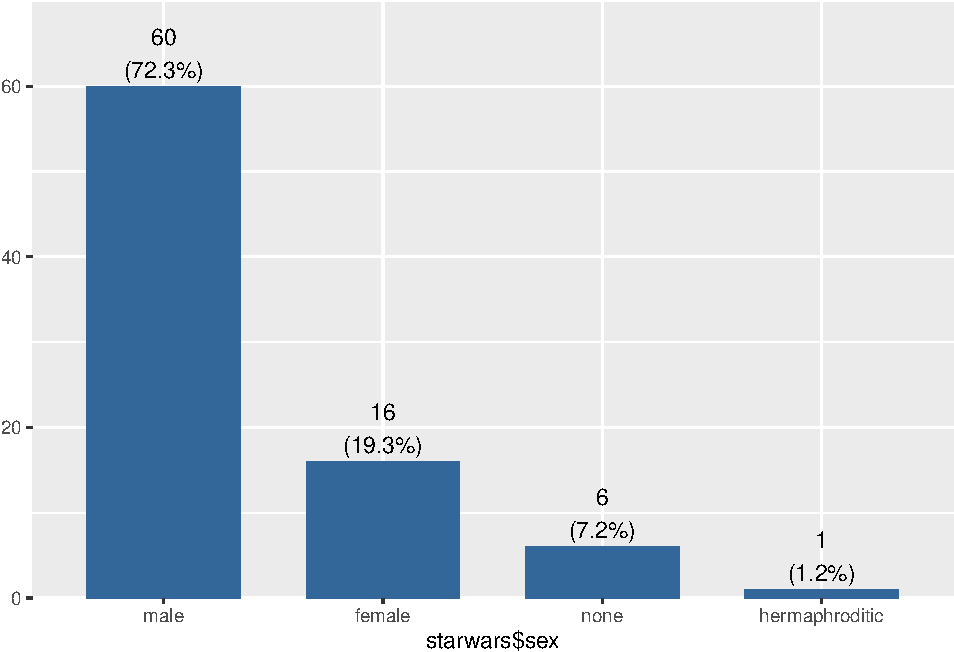
\includegraphics{r_book_files/figure-latex/freq_plot-1.pdf}

Das Argument \texttt{sort.frq\ =\ "desc"} sorgt für eine absteigende Sortierung der Balken. Es ist natürlich nur bei nominalen Daten sinnvoll.

Über die Funktion \texttt{plot\_frq()} sind noch weitere Darstellungsformen möglich, wie beispielsweise ein Liniendiagramm oder ein Diagramm mit Punkten. Man muss dazu lediglich das zusätzliche Argument \texttt{type} mit an die Funktion übergeben (z.B. \texttt{type\ =\ "line"} oder \texttt{type\ =\ "dot"}). Auch Histogramme sind möglich (\texttt{type\ =\ "histogram}):

\begin{Shaded}
\begin{Highlighting}[]
\FunctionTok{library}\NormalTok{(sjPlot)}

\FunctionTok{plot\_frq}\NormalTok{(starwars}\SpecialCharTok{$}\NormalTok{mass, }\AttributeTok{type =} \StringTok{"histogram"}\NormalTok{)}
\end{Highlighting}
\end{Shaded}

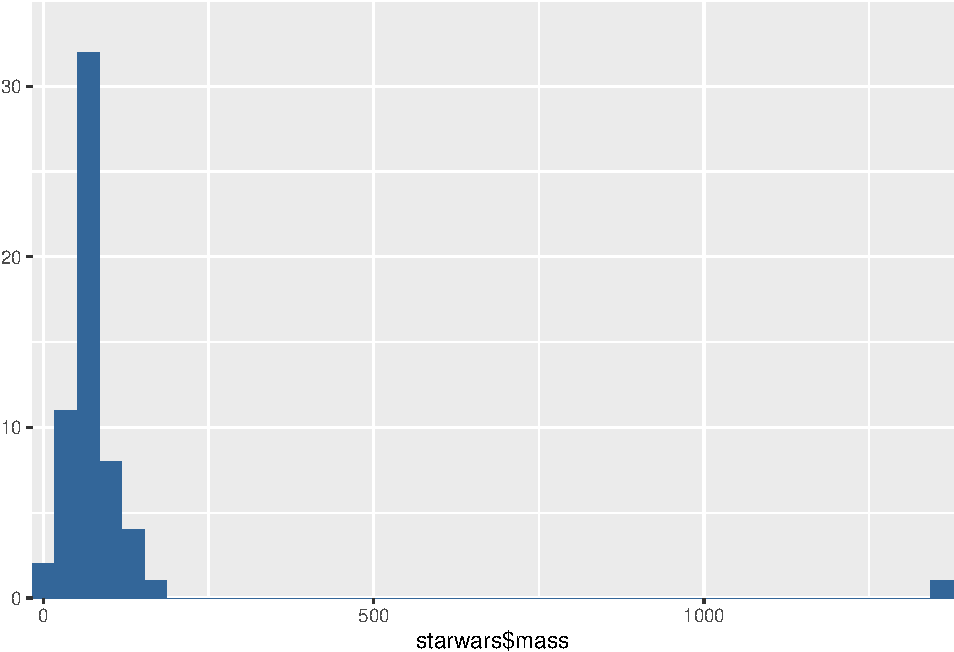
\includegraphics{r_book_files/figure-latex/freq_plot2-1.pdf}
Das Histogramm offenbart in der Variable \texttt{mass} einen extremen Ausreißer, der sehr viel schwerer ist als alle anderen Starwars-Figuren.

\hypertarget{mauxdfe-der-zentralen-tendenz-streuung}{%
\section{Maße der zentralen Tendenz \& Streuung}\label{mauxdfe-der-zentralen-tendenz-streuung}}

Neben Häufigkeitsauszählungen dienen Maße der zentralen Tendenz und Streuung dazu, die Eigenschaften von Variablen sehr kompakt zu beschreiben. Ich ordne die Maßzahlen hier nach Datenniveau, beginnend bei niedrigsten bis zum höchsten. Selbstverständlich können Sie die Maße für ein niedrigeres Datenniveau auch für höhere Datenniveaus anwenden. Umgekehrt ist das jedoch nicht sinnvoll! Allerdings kennt R das Datenniveau der Variablen nicht. Es wird also ohne Probleme und Fehlermeldung auch ein arithmetisches Mittel für eine nominale Variable ausgeben, falls diese mit Zahlen codiert wurde (bei reinen character-Variablen geht das selbstverständlich nicht). Das Denken kann uns R an dieser Stelle also leider nicht abnehmen. Wir müssen immer selbst vorab beurteilen, ob eine Berechnung sinnvoll ist oder nicht.

\hypertarget{nominale-daten}{%
\subsection{Nominale Daten}\label{nominale-daten}}

Als Beispiel für eine nominale Variable verwende ich die Frage, welches Geschlecht die Starwars-Figuren haben. Die Variable hat die folgenden Ausprägungen:

\begin{Shaded}
\begin{Highlighting}[]
\NormalTok{sjlabelled}\SpecialCharTok{::}\FunctionTok{get\_labels}\NormalTok{(starwars}\SpecialCharTok{$}\NormalTok{sex)}
\end{Highlighting}
\end{Shaded}

\begin{verbatim}
## [1] "male"           "none"           "female"         "hermaphroditic"
## [5] NA
\end{verbatim}

Der \textbf{Modus} ist der Wert in einer Verteilung, der am häufigsten vorkommt. Da die Reihenfolge der Ausprägungen dabei keine Rolle spielt, ist er sogar für nominale Daten anwendbar. Man kann ihn aber auch für ordinale und metrische Daten ermitteln.

Für den Modus gibt es in base-R keine Standard-Funktion, vielleicht ist er einfach zu simpel. Man kann den Modus einfach über eine Häufigkeitsauszählung ermitteln oder über ein Säulendiagram (siehe voriger Abschnitt).

Alternativ gibt es noch eine \texttt{Mode()}-Funktion im \texttt{DescTools}-Paket. Achtung! Das Paket ist etwas altmodisch bei der Benennung seiner Funktionen: \texttt{Mode()} muss hier zwingend groß geschrieben werden!! Außerdem liefert die Funktion kein Ergebnis zurück, wenn es zwei gleich hohe höchste Ausprägungen gibt.

\begin{Shaded}
\begin{Highlighting}[]
\FunctionTok{library}\NormalTok{(DescTools)}

\FunctionTok{Mode}\NormalTok{(starwars}\SpecialCharTok{$}\NormalTok{sex, }\AttributeTok{na.rm =} \ConstantTok{TRUE}\NormalTok{)}
\end{Highlighting}
\end{Shaded}

\begin{verbatim}
## [1] "male"
## attr(,"freq")
## [1] 60
\end{verbatim}

Die Funktion liefert gleich zwei Ergebnisse zurück: Zum einen den Wert, der die meisten Ausprägungen auf sich vereint, in diesem Fall die Ausprägung ``male''. Zum anderen die absolute Häufigkeit, die diese Ausprägung hat (n = 60).

\hypertarget{ordinale-daten}{%
\subsection{Ordinale Daten}\label{ordinale-daten}}

Der \textbf{Median} teilt die (sortierten) Fälle einer Variablen in zwei gleich große Hälften. Er kann für ordinale und metrische Daten berechnet werden.

Die Funktion für den Median gibt es sogar in base-R. Sie heißt schlicht \texttt{median()}. Die Funktion benötigt zwei Argumente. Zum einen selbstverständlich den Verweis auf die Variable und zum anderen einen Hinweis, wie mit fehlenden Werten umgegangen werden soll. Da R nicht wissen kann, wie fehlende Werte einzuberechnen wären, müssen sie vorab aus der Analyse entfernt werden, mit \texttt{na.rm\ =\ TRUE} (\emph{NA remove}).

Im Datensatz gibt es keine ordinale Variable, deshalb nehme ich im folgenden die Größe in cm (metrisch) als Beispiel:

\begin{Shaded}
\begin{Highlighting}[]
\FunctionTok{median}\NormalTok{(starwars}\SpecialCharTok{$}\NormalTok{height, }\AttributeTok{na.rm =} \ConstantTok{TRUE}\NormalTok{)}
\end{Highlighting}
\end{Shaded}

\begin{verbatim}
## [1] 180
\end{verbatim}

Die \textbf{Spannweite} (\emph{range}) gibt an, zwischen welchen Ausprägungen sich eine Variable bewegt, also den höchsten und den niedrigsten Wert.

\begin{Shaded}
\begin{Highlighting}[]
\FunctionTok{range}\NormalTok{(starwars}\SpecialCharTok{$}\NormalTok{height, }\AttributeTok{na.rm =} \ConstantTok{TRUE}\NormalTok{)}
\end{Highlighting}
\end{Shaded}

\begin{verbatim}
## [1]  66 264
\end{verbatim}

Über die Funktionen \texttt{min()} und \texttt{max()} kann man sich übrigens auch einzeln das Minimum bzw. Maximum ausgeben lassen.

Wie oben erwähnt, teilt der Median die Verteilung der Werte in zwei gleiche Hälften. Wenn man jedoch nicht zwei Hälften haben möchte, sondern sich eher für Drittel, Viertel oder Fünftel interessiert, sind \textbf{Quantile} das Mittel der Wahl. Üblich sind eigentlich nur Quartile, also die Einteilung in Viertel. Deshalb gibt die base-R-Funktion \texttt{quantile()} standardmäßig die Grenzen der Quartile zurück.

\begin{Shaded}
\begin{Highlighting}[]
\FunctionTok{quantile}\NormalTok{(starwars}\SpecialCharTok{$}\NormalTok{height, }\AttributeTok{na.rm =} \ConstantTok{TRUE}\NormalTok{)}
\end{Highlighting}
\end{Shaded}

\begin{verbatim}
##   0%  25%  50%  75% 100% 
##   66  167  180  191  264
\end{verbatim}

Es handelt sich um 5 Grenzen, weil der niedrigste und der höchste Wert mit ausgegeben werden. Die Quartile befinden sich quasi ``zwischen'' diesen 5 Grenzpunkten.

Der **Interquartilsabstand* gibt den Abstand zwischen dem Ende des ersten und dem Beginn des letzten Quartils an, also in unserem Beispiel den Abstand zwischen den Ausprägungen 167 und 191 cm (= 24 cm).

\begin{Shaded}
\begin{Highlighting}[]
\FunctionTok{IQR}\NormalTok{(starwars}\SpecialCharTok{$}\NormalTok{height, }\AttributeTok{na.rm =} \ConstantTok{TRUE}\NormalTok{)}
\end{Highlighting}
\end{Shaded}

\begin{verbatim}
## [1] 24
\end{verbatim}

\hypertarget{metrische-daten}{%
\subsection{Metrische Daten}\label{metrische-daten}}

Für metrische Variablen haben Sie die Auswahl zwischen allen hier vorgestellten Maßen der zentralen Tendenz (wobei der Modus in der Regel bei vielen Ausprägungen kaum Sinn macht). Üblich ist vor allem das \textbf{``arithmetische Mittel''}, umgangssprachlich oft auch als Durchschnitt oder Mittelwert bezeichnet. Die Funktion \texttt{mean()} habe ich in den Einführungskapiteln bereits als Beispiel genutzt.

Als Beispiel benutze ich hier die Variable für das Gewicht.

\begin{Shaded}
\begin{Highlighting}[]
\FunctionTok{mean}\NormalTok{(starwars}\SpecialCharTok{$}\NormalTok{mass, }\AttributeTok{na.rm =} \ConstantTok{TRUE}\NormalTok{)}
\end{Highlighting}
\end{Shaded}

\begin{verbatim}
## [1] 97,31186
\end{verbatim}

Das Durschnittsgewicht im Sample beträgt also 97.31 Einheiten (kg?).

Man kann sich auch ein \textbf{getrimmtes Mittel} ausgeben lassen, bei dem die oberen und niedrigen X Prozent der Daten entfernt werden. So kann das arithmetische Mittel robust gemacht werden gegen Extremwerte. Aus dem Abschnitt über die Häufigkeiten (Histogram) wissen wir, dass es in der Variable einen extremen Ausreißer gibt. Ein Starwars-Charakter ist viel schwerer als alle anderen. Er verzerrt das arithmetische Mittel nach oben. Ein getrimmtes Mittel liefert deshalb vielleicht ein realistischeres Bild:

\begin{Shaded}
\begin{Highlighting}[]
\FunctionTok{mean}\NormalTok{(starwars}\SpecialCharTok{$}\NormalTok{mass, }\AttributeTok{trim =} \FloatTok{0.1}\NormalTok{, }\AttributeTok{na.rm =} \ConstantTok{TRUE}\NormalTok{)}
\end{Highlighting}
\end{Shaded}

\begin{verbatim}
## [1] 75,43673
\end{verbatim}

Es macht Sinn, sich bei einer Variable nie allein das arithmetische Mittel anzusehen. Sie wüssten dann z.B. nicht ob ein Wert (z.B. 80 kg) nur erreicht wird, weil alle Befragten genau so schwer sind, weil es sehr viele Personen mit 75 und 85 kg im Sample gibt oder eine ganz andere Verteilung vorherrscht. Wie der Name schon sagt, geben \textbf{Streuungsmaße} Auskunft darüber, wie die Werte einer Variablen um den Mittelwert streuen oder variieren. Das wichtigste Streuungsmaß, welches auch immer gemeinsam mit dem arithmetischen Mittel angesehen und berichtet werden sollte, ist die \textbf{Streuung} (\emph{standard deviation}).

\begin{Shaded}
\begin{Highlighting}[]
\FunctionTok{sd}\NormalTok{(starwars}\SpecialCharTok{$}\NormalTok{mass, }\AttributeTok{na.rm =} \ConstantTok{TRUE}\NormalTok{)}
\end{Highlighting}
\end{Shaded}

\begin{verbatim}
## [1] 169,4572
\end{verbatim}

Die Streuung ist bekanntlich die Wurzel der Varianz und als Streuungsmaß auch um einiges üblicher. Dennoch soll hier natürlich auch die Funktion für die Varianz nicht fehlen:

\begin{Shaded}
\begin{Highlighting}[]
\FunctionTok{var}\NormalTok{(starwars}\SpecialCharTok{$}\NormalTok{mass, }\AttributeTok{na.rm =} \ConstantTok{TRUE}\NormalTok{)}
\end{Highlighting}
\end{Shaded}

\begin{verbatim}
## [1] 28715,73
\end{verbatim}

\hypertarget{schiefe-und-kurtosis}{%
\section{Schiefe und Kurtosis}\label{schiefe-und-kurtosis}}

Weitere Kennwerte für die Form von Verteilungen sind die \textbf{Schiefe} (\emph{skew}) und \textbf{Kurtosis} (\emph{kurtosis}). Die Schiefe ist quasi das Gegenteil von Symmetrie. Kurtosis drückt aus, wie spitz (nach oben gewölbt) oder flach eine Verteilung ist.

Im \texttt{psych}-Paket gibt es Funktionen für beides:

\begin{Shaded}
\begin{Highlighting}[]
\FunctionTok{library}\NormalTok{(psych)}
\FunctionTok{skew}\NormalTok{(starwars}\SpecialCharTok{$}\NormalTok{height, }\AttributeTok{na.rm =} \ConstantTok{TRUE}\NormalTok{)}
\end{Highlighting}
\end{Shaded}

\begin{verbatim}
## [1] -1,025488
\end{verbatim}

Zur Erinnerung:

\begin{itemize}
\item
  Ist die Schiefe \textgreater{} 0 so ist die Verteilung rechtsschief (Modus \textless{} Median \textless{} arithmetisches Mittel).
\item
  Ist die Schiefe = 0, so ist die Verteilung symmetrisch (Modus = Median = arithmetisches Mittel).
\item
  Ist die Schiefe \textless{} 0 so ist die Verteilung linksschief (Modus \textgreater{} Median \textgreater{} arithmetisches Mittel).
\end{itemize}

Die Verteilung des Alters im obigen Beispiel ist also nahezu symmetrisch, ein wenig linksschief.

Hier noch der Code zur Berechnung der Kurtosis:

\begin{Shaded}
\begin{Highlighting}[]
\FunctionTok{kurtosi}\NormalTok{(starwars}\SpecialCharTok{$}\NormalTok{height, }\AttributeTok{na.rm =} \ConstantTok{TRUE}\NormalTok{)}
\end{Highlighting}
\end{Shaded}

\begin{verbatim}
## [1] 1,776414
\end{verbatim}

\hypertarget{uxfcbersichts-funktionen}{%
\section{Übersichts-Funktionen}\label{uxfcbersichts-funktionen}}

Bisher haben wir uns die Statistiken jeweils für eine einzelne Variable ausgeben lassen. Aber natürlich macht es Sinn, sich mehrere Kennwerte gleichzeitig ausgeben zu lassen. Die Funktion \texttt{summary()} aus dem base-Paket liefert zum Beispiel einen guten ersten Einblick:

\begin{Shaded}
\begin{Highlighting}[]
\FunctionTok{summary}\NormalTok{(starwars}\SpecialCharTok{$}\NormalTok{height)}
\end{Highlighting}
\end{Shaded}

\begin{verbatim}
##    Min. 1st Qu.  Median    Mean 3rd Qu.    Max.    NA's 
##    66,0   167,0   180,0   174,4   191,0   264,0       6
\end{verbatim}

Allerdings fehlen an dieser Stelle z.B. die Streuungsmaße. Es geht also noch mehr. Das vorhin genutzte \texttt{psych}-Paket hat z.B. eine \texttt{describe()}-Funktion, mit der man sich gleichzeitig verschiedene deskriptive Statistiken ausgeben kann - und zwar nicht nur für eine Variable, sondern gleich für mehrere oder sogar für einen ganzen Datensatz.

In dem nun folgenden Code habe ich den Datensatz um ein paar Variablen gekürzt (\texttt{{[},\ 1:11{]}}), weil die Funktion \texttt{describe()} mit diesen Variablen nicht funktioniert.

\begin{Shaded}
\begin{Highlighting}[]
\NormalTok{desc\_stats }\OtherTok{\textless{}{-}} \FunctionTok{describe}\NormalTok{(starwars[, }\DecValTok{1}\SpecialCharTok{:}\DecValTok{11}\NormalTok{])}
\FunctionTok{head}\NormalTok{(desc\_stats)}
\end{Highlighting}
\end{Shaded}

\begin{verbatim}
##             vars  n   mean     sd median trimmed   mad min  max range  skew
## name*          1 87  44,00  25,26     44   44,00 32,62   1   87    86  0,00
## height         2 81 174,36  34,77    180  178,17 19,27  66  264   198 -1,03
## mass           3 59  97,31 169,46     79   75,44 16,31  15 1358  1343  6,97
## hair_color*    4 82   7,94   2,70     10    8,12  2,97   1   12    11 -0,58
## skin_color*    5 87  13,62   8,26     13   13,15  8,90   1   31    30  0,47
## eye_color*     6 87   6,25   4,83      4    5,86  4,45   1   15    14  0,67
##             kurtosis    se
## name*          -1,24  2,71
## height          1,78  3,86
## mass           48,93 22,06
## hair_color*    -0,83  0,30
## skin_color*    -0,93  0,89
## eye_color*     -1,04  0,52
\end{verbatim}

Da sind jetzt sogar einige Kennzahlen dabei, die wir bisher gar nicht besprochen haben (und auch nicht besprechen werden, z.B. ``mad''). Über verschiedene Argumente kann man sich noch weitere Kennzahlen in der Tabelle anzeigen lassen (z.B. \texttt{skew\ =\ TRUE} oder \texttt{ranges\ =\ TRUE}). Allerdings fällt auch auf, dass die Berechnungen nicht für alle Variablen durchgeführt werden. Ein Mittelwert der Namen ist auch keine nützliche Angabe. Mit dem zusätzlichen Argument \texttt{omit\ =\ TRUE} kann man diese Zeilen ausblenden.

Kleine Warnung: Die RStudio-Cloud verhält sich in Bezug auf die describe()-Funktion leicht anders. Warum das so ist, weiß ich nicht.

\hypertarget{wichtige-funktionen-aus-diesem-kapitel-2}{%
\section*{Wichtige Funktionen aus diesem Kapitel}\label{wichtige-funktionen-aus-diesem-kapitel-2}}
\addcontentsline{toc}{section}{Wichtige Funktionen aus diesem Kapitel}

\begin{longtable}[]{@{}llll@{}}
\toprule
Funktion & Paket & Beschreibung & Wichtige Argumente\tabularnewline
\midrule
\endhead
\textbf{Häufigkeiten} & & &\tabularnewline
\texttt{table()} & stats & einfache Tabelle & \texttt{useNA\ =\ "ifany"}\tabularnewline
\texttt{tabyl()} & janitor & Häufigkeitstabelle mit Prozent &\tabularnewline
\texttt{plot\_frq()} & sjPlot & Säulendiagramm &\tabularnewline
\textbf{Maße der zentralen Tendenz \& Streuung} & & &\tabularnewline
\texttt{Mode()} & DescTools & Modus &\tabularnewline
\texttt{median()} & stats & Median & \texttt{na.rm\ =\ TRUE}\tabularnewline
\texttt{range()} & stats & Range & \texttt{na.rm\ =\ TRUE}\tabularnewline
\texttt{quantile()} & stats & Quantilgrenzen & \texttt{na.rm\ =\ TRUE}\tabularnewline
\texttt{IQR()} & stats & Inter-Quartil-Range & \texttt{na.rm\ =\ TRUE}\tabularnewline
\texttt{mean()} & base & Arithmetisches Mittel & \texttt{na.rm\ =\ TRUE}\tabularnewline
\texttt{sd()} & stats & Standardabweichung & \texttt{na.rm\ =\ TRUE}\tabularnewline
\texttt{var()} & stats & Varianz & \texttt{na.rm\ =\ TRUE}\tabularnewline
\textbf{Schiefe und Kurtosis} & & &\tabularnewline
\texttt{skew()} & psych & Schiefe & \texttt{na.rm\ =\ TRUE}\tabularnewline
\texttt{kurtosi()} & psych & Kurtosis & \texttt{na.rm\ =\ TRUE}\tabularnewline
\textbf{Übersichts-Funktionen} & & &\tabularnewline
\texttt{summary()} & base & Wichtige Verteilungsmerkmale &\tabularnewline
\texttt{describe()} & psych & Tabelle deskriptiver Merkmale &\tabularnewline
\bottomrule
\end{longtable}

\hypertarget{bivariate-statistik}{%
\chapter{Bivariate Statistik}\label{bivariate-statistik}}

In diesem Kapitel geht es um bivariate Verfahren, also die gemeinsame Variation von zwei Variablen. Im Detail behandeln wir hier die Kreuztabelle und Chi-Quadrat sowie die Korrelation.

\hypertarget{kreuztabellen}{%
\section{Kreuztabellen}\label{kreuztabellen}}

Mit Kreuztabellen/Kontingenztabellen kann man die Verteilung einer Variable unter Berücksichtigung einer anderen in den Blick nehmen. Damit die Tabelle übersichtlich bleibt, sollten beide Variablen eher wenige Ausprägungen haben, also eher nominales oder ordinales Datenniveau haben.

Chi-Quadrat ist eine Maßzahl für die Differenz zwischen der Kontingenztabelle (=gemessene Werte) und der Indifferenztabelle (=die Tabelle die entstünde, wenn es keinen Zusammenhang zwischen den Variablen geben würde). Ist Chi-Quadrat = 0, besteht kein Zusammenhang zwischen den Variablen. Allerdings kann Chi-Quadrat abhängig von der Reihen- und Spaltenzahl, sowie der Fallzahl, unendlich hohe Werte annehmen. Chi-Quadrate für unterschiedliche Tabellen lassen sich deshalb schlecht vergleichen. Mit Cramer´s V liegt eine standardisierte Form von Chi-Quadrat vor, die zwischen 0 und 1 variiert. Über die Richtung von Zusammenhängen gibt aber auch Cramer´s V keine Auskunft. Dazu muss man in der Kreuztabelle nachsehen. Kreuztabellen und Chi-Quadrat-basierte Maßzahlen sind bei Hypothesentests immer dann das Mittel der Wahl, wenn die abhängige Variable nominales Datenniveau hat.

Im Folgenden verwende ich wieder den Geneartion-Z-Datensatz als Beispiel. Darin gibt es einige Variablen zur politischen Partizipation, z.B. ob man schon einmal an einer Wahl teilgenommen hat oder schon einmal eine Petition unterschrieben hat. Diese Variablen sind dichotom 0/1-codiert. Die ``0'' bedeutet dabei, dass ein:e Befragte:r die Partizipationsmöglichkeit noch nie wahrgenommen hat und ``1'' bedeutet, dass sie mindestens einmal wahrgenommen wurde.

Außerdem enthält der Datensatz noch die Variable ``alter\_g3'', die ich in drei Gruppen eingeteilt habe (``14 bis 17 Jahre'', ``18 bis 21 Jahre'' und ``22 bis 24 Jahre'').

\begin{Shaded}
\begin{Highlighting}[]
\FunctionTok{head}\NormalTok{(data)}
\end{Highlighting}
\end{Shaded}

\begin{verbatim}
## # A tibble: 6 x 13
##    lfdn alter_g3         pol_part_wahl pol_part_petition pol_part_sm_kommentar
##   <dbl> <chr>                <dbl+lbl>         <dbl+lbl>             <dbl+lbl>
## 1  1634 22 bis 24 Jahre 0 [not quoted]    0 [not quoted]        0 [not quoted]
## 2  1636 22 bis 24 Jahre 1 [quoted]        0 [not quoted]        1 [quoted]    
## 3  1637 22 bis 24 Jahre 1 [quoted]        1 [quoted]            0 [not quoted]
## 4  1638 22 bis 24 Jahre 1 [quoted]        1 [quoted]            0 [not quoted]
## 5  1639 22 bis 24 Jahre 1 [quoted]        0 [not quoted]        0 [not quoted]
## 6  1640 22 bis 24 Jahre 1 [quoted]        1 [quoted]            0 [not quoted]
## # ... with 8 more variables: pol_part_partei_veranstaltung <dbl+lbl>,
## #   pol_part_demo <dbl+lbl>, pol_part_information <dbl+lbl>,
## #   pol_part_gespraech <dbl+lbl>, pol_part_produktboykott <dbl+lbl>,
## #   pol_part_parteiengagement <dbl+lbl>, pol_part_anderes_engagement <dbl+lbl>,
## #   pol_part_nichts_davon <dbl+lbl>
\end{verbatim}

Ziel des nachfolgenden Skriptes ist es zu eruieren, ob sich der Anteil derjenigen, die eine Partizipationsmöglichkeit wahrgenommen haben, zwischen den Altersgruppen unterscheidet. Die Vermutung (Hypothese), die darin steckt ist natürlich, dass bei zunehmendem Alter der Anteil derjenigen steigt, die diese Möglichkeit bereits wahrgenommen haben. Das Beispiel hier im Buch beschäftigt sich insbesondere mit dem Unterschreiben von Petitionen.

Unsere H1 lautet also:

\emph{Der Anteil derjenigen, die bereits eine Petition unterschrieben haben, steigt mit zunehmendem Alter.}

Bevor es mit dem Hypothesentest losgehen kann, müssen die erforderlichen Pakete geladen werden. Das tidyverse für die Pipe, \texttt{janitor} für die Kreuztabellen und Chi-Quadrat (χ2) und \texttt{DescTools} für Cramer´s V.

\begin{Shaded}
\begin{Highlighting}[]
\FunctionTok{library}\NormalTok{(tidyverse)}
\FunctionTok{library}\NormalTok{(janitor)}
\FunctionTok{library}\NormalTok{(DescTools)}
\end{Highlighting}
\end{Shaded}

\hypertarget{vorbereitung-univariate-verteilung}{%
\subsection{Vorbereitung: Univariate Verteilung}\label{vorbereitung-univariate-verteilung}}

Schauen wir uns zunächst einmal die univariate Verteilung der beiden Variablen an.
Dies ist hilfreich, um ein Gefühl für die Daten zu bekommen und ein Verständnis dafür zu entwickeln, welche Verteilung wir erwarten würden.
Das geht (wie im Kapitel zu den Häufigkeitstabellen beschrieben) am schönsten mit dem Paket \texttt{janitor} und der Funktion \texttt{tabyl()}.

\begin{Shaded}
\begin{Highlighting}[]
\CommentTok{\# Häufigkeitstabelle Altersgruppen}
\FunctionTok{tabyl}\NormalTok{(data}\SpecialCharTok{$}\NormalTok{alter\_g3)}
\end{Highlighting}
\end{Shaded}

\begin{verbatim}
##    data$alter_g3   n   percent
##  14 bis 17 Jahre 356 0,3542289
##  18 bis 21 Jahre 354 0,3522388
##  22 bis 24 Jahre 295 0,2935323
\end{verbatim}

Die drei Altersgruppen sind also alle etwa gleich stark besetzt, die älteste Altersgruppe ist ca. 5 Prozent kleiner als die anderen beiden.

Jetzt noch die Beteiligung an Petitionen:

\begin{Shaded}
\begin{Highlighting}[]
\CommentTok{\# Häufigkeitstabelle Teilnahme Petitionen}
\FunctionTok{tabyl}\NormalTok{(data}\SpecialCharTok{$}\NormalTok{pol\_part\_petition)}
\end{Highlighting}
\end{Shaded}

\begin{verbatim}
##  data$pol_part_petition   n   percent
##                       0 680 0,6766169
##                       1 325 0,3233831
\end{verbatim}

Ein knappes Drittel der Befragten haben bereits eine Petition unterschrieben. Würde kein Zusammenhang/Unterschied in den Gruppen vorliegen, wäre also zu erwarten, dass etwa ein Drittel der Befragten in jeder Altersgruppe bereits eine Petition unterschrieben hat.

\hypertarget{kreuztabelle-ausgeben}{%
\subsection{Kreuztabelle ausgeben}\label{kreuztabelle-ausgeben}}

Mit dem Paket \texttt{janitor} und der Funktion \texttt{tabyl()} kann man nicht nur einfache Tabellen erstellen, sondern auch Kreuztabellen. Dazu gibt man die beiden Variablen, die man kreuztabulieren möchte, einfach nacheinander als Argumente in die Funktion. Die Variable, die zuerst übergeben wird, steht dann hinterher in den Zeilen, die zweite in den Spalten. Es ist eine Konvention, dass Variablen, die als unabhängig betrachtet werden, bei Kreuztabellen in den Spalten dargestellt werden. An einigen Stellen findet man es aber auch andersherum. Das Layout einer Tabelle hängt ja auch manchmal davon ab, wo man wieviel Platz hat und wenn man eine unabhängige Variable mit sehr vielen Ausprägungen hat, dann passt sie unter Umständen besser in die Zeilen.

Wir halten uns im folgenden Code jedoch an die Konvention und übergeben zusätzlich noch das Argument \texttt{show\_na\ =\ FALSE} um fehlende Werte aus der Analyse auszuschließen.

Hier der Basis-Code für die Kreuztabelle mit \texttt{janitor::tabyl()}:

\begin{Shaded}
\begin{Highlighting}[]
\CommentTok{\# Kreuztabelle berechnen}
\NormalTok{my\_crosstab }\OtherTok{\textless{}{-}}\NormalTok{ data }\SpecialCharTok{\%\textgreater{}\%}
\NormalTok{  janitor}\SpecialCharTok{::}\FunctionTok{tabyl}\NormalTok{(pol\_part\_petition, alter\_g3, }\AttributeTok{show\_na =} \ConstantTok{FALSE}\NormalTok{) }

\NormalTok{my\_crosstab}
\end{Highlighting}
\end{Shaded}

\begin{verbatim}
##  pol_part_petition 14 bis 17 Jahre 18 bis 21 Jahre 22 bis 24 Jahre
##                  0             284             213             183
##                  1              72             141             112
\end{verbatim}

Die Tabelle macht genau was sie soll, sie tabuliert die beiden Variablen im vorgegebenen Layout und gibt dabei die absoluten Häufigkeiten aus. Jetzt wäre es natürlich schön, wenn wir die Tabelle weiter formatieren können und z.B. Prozentwerte und auch Randspalten hinzufügen könnten. Das geht natürlich auch. Dazu beinhaltet das \texttt{janitor}-Paket eine Reihe von Funktionen, die alle mit \texttt{adorn\_} beginnen, z.B.:

\begin{itemize}
\item
  \texttt{adorn\_totals()} fügt Randhäufigkeiten hinzu. Mit dem Argument \texttt{where\ =} kann man noch bestimmen, ob dies in den Spalten (\texttt{"col"}), oder in den Reihen (\texttt{"row"}) oder in beidem \texttt{c("row",\ "col")} geschehen soll.
\item
  \texttt{adorn\_percentages()} berechnet die Prozentwerte. Mit dem Argument \texttt{denominator\ =} kann man noch bestimmen, ob dies in den Spalten (\texttt{"col"}), oder in den Reihen (\texttt{"row"}) oder in beidem \texttt{"all"} geschehen soll.
\item
  \texttt{adorn\_pct\_formatting()} dient der Formatierung der Prozentwerte. Über das Argument \texttt{digits\ =} kann man die Anzahl der Nachkommastellen festlegen.
\item
  \texttt{adorn\_ns()} fügt die absoluten Häufigkeiten wieder hinzu. Denn diese werden bei der Formatierung in Prozentwerte durch \texttt{adorn\_percentages()} überschreiben.
\item
  \texttt{adorn\_title()} dient zur Beschriftung der Tabelle. Mit \texttt{placement\ =\ "combined"} kann man z.B. in der ersten Zelle kombiniert die beiden Variablennamen anzeigen lassen. Mit der Variante \texttt{placement\ =\ "top"} wird die Beschriftung in einer Zeile darüber eingetragen.
\end{itemize}

Probieren wir es aus:

\begin{Shaded}
\begin{Highlighting}[]
\CommentTok{\# Kreuztabelle formatieren}
\NormalTok{my\_crosstab }\SpecialCharTok{\%\textgreater{}\%} 
  \FunctionTok{adorn\_totals}\NormalTok{(}\AttributeTok{where =} \FunctionTok{c}\NormalTok{(}\StringTok{"row"}\NormalTok{, }\StringTok{"col"}\NormalTok{)) }\SpecialCharTok{\%\textgreater{}\%}
  \FunctionTok{adorn\_percentages}\NormalTok{(}\AttributeTok{denominator =} \StringTok{"col"}\NormalTok{) }\SpecialCharTok{\%\textgreater{}\%} 
  \FunctionTok{adorn\_pct\_formatting}\NormalTok{(}\AttributeTok{digits =} \DecValTok{0}\NormalTok{) }\SpecialCharTok{\%\textgreater{}\%}
  \FunctionTok{adorn\_ns}\NormalTok{() }\SpecialCharTok{\%\textgreater{}\%}
  \FunctionTok{adorn\_title}\NormalTok{(}\AttributeTok{placement =} \StringTok{"top"}\NormalTok{)}
\end{Highlighting}
\end{Shaded}

\begin{verbatim}
##                           alter_g3                                            
##  pol_part_petition 14 bis 17 Jahre 18 bis 21 Jahre 22 bis 24 Jahre       Total
##                  0       80% (284)       60% (213)       62% (183)  68%  (680)
##                  1       20%  (72)       40% (141)       38% (112)  32%  (325)
##              Total      100% (356)      100% (354)      100% (295) 100% (1005)
\end{verbatim}

Sehr hübsch! Durch die übersichtliche Formatierung mit den Prozentwerten können wir jetzt gut vergleichen, wie sich der Anteil derjenigen, die bereits Petitionen unterschreiben haben in den Altersgruppen unterscheidet. Zur Erinnerung, im Gesamten Sample waren es 32 Prozent, die diese Form der politischen Partizipation bereits genutzt haben (siehe auch Spalte ``Total'').

Vergleicht man nun die Altersgruppen sieht man deutliche Unterschiede:

\begin{itemize}
\item
  Insbesondere die erste Gruppe der 14- bis 17-Jährigen hat deutlich weniger Petitionen unterschrieben, als die anderen beiden Gruppen. Dies war erwartbar und entspricht im auch der Hypothese, die wir eingangs formuliert hatten. Möglicherweise spielt für diese Art der politischen Partizipation die Volljährigkeit eine besondere Rolle?
\item
  Zwischen den älteren beiden Altersgruppen ist hingegen kaum ein Unterschied. Der Prozentsatz sinkt sogar leicht ab, was unserer Hypothese nicht entsprechen würde. Allerdings ist die Differenz ohnehin sehr gering und kaum von Bedeutung.
\end{itemize}

Nach dem Augenschein der Kreuztabelle, scheinen wir also insgesamt auf einen interessanten Zusammenhang gestoßen zu sein, der unserer Hypothese auch entspricht. Aber ist dieser Zusammenhang auch signifikant?

\hypertarget{chi-quadrat-cramers-v}{%
\subsection{Chi-Quadrat \& Cramer´s V}\label{chi-quadrat-cramers-v}}

Dazu ziehen wir im folgenden den Chi-Quadrat-Test heran, ebenfalls aus dem Paket \texttt{janitor}.

\begin{Shaded}
\begin{Highlighting}[]
\CommentTok{\# Chi{-}Quadrat berchnen}
\NormalTok{janitor}\SpecialCharTok{::}\FunctionTok{chisq.test}\NormalTok{(my\_crosstab)}
\end{Highlighting}
\end{Shaded}

\begin{verbatim}
## 
##  Pearson's Chi-squared test
## 
## data:  my_crosstab
## X-squared = 37,226, df = 2, p-value = 8,249e-09
\end{verbatim}

Chi-Quadrat beträgt 37.2 (df = 2), bei einem sehr kleinen p-Wert. Der p-Wert 8.249e-09 bedeutet 8.249 * 10 \^{} -9 also 0.000000008249. Das ist deutlich unter p \textless{} .001 und damit ``signifikant''. Wir können deshalb davon ausgehen, dass der Zusammenhang/Unterschied, den wir hier beobachtet haben, überzufällig zu Stande gekommen ist. Die Daten unterstützen also unsere Hypothese H1.

Aber wie stark ist der gefundene Zusammenhang? Dabei hilft uns Cramer´s V, quasi das standardisierte Chi-Quadrat. Die Funktion dazu findet sich im Paket \texttt{DescTools} und heißt \texttt{CramerV()}. Sie benötigt als einziges Argument eine Kreuztabelle, bzw. die darin befindlichen Zahlen als Matrix (also auf keinen Fall die formatierte Tabelle). Die einfache Tabelle haben wir oben im Objekt \texttt{my\_crosstab} gespeichert. Für die Berechnung von Cramer´s V muss noch die erste Spalte gelöscht werden, die die Ausprägungen der Variable zu Petitionen enthält. Über das Subsetting \texttt{{[},\ -1{]}} können wir genau dies erreichen. Der Befehl besagt quasi: Gib alle Zeilen aus (durch das Weglassen der Angabe vor dem Komma - wenn man hier nichts schreibt, bdeutet das ``keine Enischränkung'') und alle Spalten bis auf die erste (nach dem Komma \texttt{-1}).

\begin{Shaded}
\begin{Highlighting}[]
\CommentTok{\# Cramer´s V}
\NormalTok{DescTools}\SpecialCharTok{::}\FunctionTok{CramerV}\NormalTok{(my\_crosstab[, }\SpecialCharTok{{-}}\DecValTok{1}\NormalTok{])}
\end{Highlighting}
\end{Shaded}

\begin{verbatim}
## [1] 0,1924605
\end{verbatim}

Cramer´s V beträgt .19. Es besteht also ein schwacher, aber signifikanter Zusammenhang zwischen dem Alter und der politischen Beteiligung mittels Petitionen.

Die Hypothese kann damit insgesamt als bestätigt angesehen werden, auch wenn wir einräumen müssen, dass nicht zwischen allen Altersgruppen Unterschiede bestehen.
Stattdessen wird offenbar durch das Erreichen der Volljährigkeit ein relevanter Anstieg beim Unterzeichnen von Petitionen befördert. Spannend!

\hypertarget{korrelationen}{%
\section{Korrelationen}\label{korrelationen}}

Dieser Abschnitt ist den Zusammenhängen zwischen metrischen Variablen gewidmet. Dabei wird zunächst auf die grafische Analyse eingegangen und dann die Berechnung der Kovarianz und des Korrelationskoeffizienten \emph{r} veranschaulicht. Dabei werden sowohl die Befehle aus base-R als auch die entsprechenden Befehle aus dem Paket \texttt{psych} verwendet. Zudem wird noch das Paket \texttt{corrr} vorgestellt, das zur explorativen grafischen Analyse von Korrelationen dient.

Zunächst werden die entsprechenden Pakete geladen.

\begin{Shaded}
\begin{Highlighting}[]
\FunctionTok{library}\NormalTok{(tidyverse) }\CommentTok{\# für Scatterplots und die Pipe}
\FunctionTok{library}\NormalTok{(psych)     }\CommentTok{\# für Korrelationen}
\FunctionTok{library}\NormalTok{(corrr)     }\CommentTok{\# für Korrelationsmatrizen}
\end{Highlighting}
\end{Shaded}

Als Datenbeispiel dient wieder der Generation-Z-Datensatz. Ich habe in diesem Datensatz zwei Indices gebildet, deren Zusammenhang wir hier untersuchen wollen.

\begin{itemize}
\item
  Für die \emph{Politische Partizipation} habe ich einen Summenindex gebildet. Er zählt, wie viele von zehn möglichen Aktivitäten der politischen Partizipation eine Person bereits ausgeführt hat (z.B. Wählen gehen, Petitionen unterschreiben, demonstrieren oder Konsumboykott).
\item
  Für die \emph{Politische Entfremdung} habe ich einen Mittelwertindex gebildet, der auf fünf Items beruht, welche jeweils auf einer 4er-Skala von 1 = \emph{stimme überhaupt nicht zu} bis 4 = \emph{stimme voll und ganz zu} gemessen wurden. (Hier drei Beispielitems: \emph{Politik hat mit meinem Leben nichts zu tun}, \emph{Entscheidungsprozesse in der Politik sind für mich meistens nicht nachvollziehbar} und \emph{Den Parteien geht es nur um Macht}).
\end{itemize}

Außerdem enthält der Datensatz noch die Variablen \texttt{lfdn} für die Fallnummer und das \texttt{alter} der Befragten.

\begin{Shaded}
\begin{Highlighting}[]
\FunctionTok{head}\NormalTok{(df)}
\end{Highlighting}
\end{Shaded}

\begin{verbatim}
## # A tibble: 6 x 4
##    lfdn pol_part_sx pol_entfremdung_ix         alter
##   <dbl>       <dbl>              <dbl>     <dbl+lbl>
## 1  1634           0                2.4 23 [23 Jahre]
## 2  1636           5                2.8 24 [24 Jahre]
## 3  1637           5                2.4 23 [23 Jahre]
## 4  1638           6                2.8 23 [23 Jahre]
## 5  1639           4                1.8 24 [24 Jahre]
## 6  1640           5                2.8 24 [24 Jahre]
\end{verbatim}

Im folgenden soll nun die folgende Hypothese getestet werden:

\emph{H1: Zwischen politischer Partizipation und politischer Entfremdung besteht ein negativer Zusammenhang.}

Diese Alternativhypothese steht im Gegensatz zur folgenden Nullhypothese:

\emph{H0: Es gibt keinen (oder sogar einen positiven) Zusammenhang zwischen politischer Partizipation und politischer Entfremdung.}

Die Nullhypothese müsste beibehalten werden, sofern wir bei der Berechnung der Korrelation einen Wert von \emph{r} berechnen, der größer oder gleich 0 ist \textbf{oder} wenn wir zwar ein negatives \emph{r} berechnen, aber der p-Wert indiziert, dass dieses berechnete \emph{r} sich nicht signifikant von 0 unterscheidet. Andernfalls können wir davon ausgehen, dass in der Grundgesamtheit wohl eher die H1 zutrifft.

\hypertarget{streudiagramm}{%
\subsection{Streudiagramm}\label{streudiagramm}}

Wir starten zunächst mit einem Streudiagramm/Scatterplot und nutzen dazu das Paket \texttt{ggplot2} aus dem tidyverse. Das Paket wird im nächsten Kapitel (ab Januar) noch ausführlicher erläutert werden. Die Funktion zum Anlegen eines Plots in ggplot2 ist \texttt{ggplot()}. Sie benötigt als erstes Argument den Datensatz und dann als zweites Argument eine Hilfsfunktion, die \texttt{aes()} heißt. Diese Funktion ist für die \emph{Ästhetik}, also das Aussehen des Plots, verantwortlich. In unserem Fall sind das die beiden Variablen, welche wir auf der X- und der Y-Achse anordnen.

Nach dem Anlegen des Plots müssen wir dem Plot noch ein \emph{Geom} hinzufügen. Der Begriff steht für \emph{geom}etrisches Objekt. Ein Geom ist im Prinzip eine Funktion für die Art der Grafik. Es beinhaltet z.B. statistische Transformationen, die zur Darstellung der Grafik nötig sind und außerdem Default-Layout-Informationen. In unserem Fall möchten wir das Geom \texttt{geom\_jitter} hinzufügen, also einen ``zitternden'' Scatterplot. Eine Übersicht über verschiedene Geome findet man \href{https://rstudio.com/wp-content/uploads/2015/06/ggplot2-german.pdf}{hier}. Das Geom wird mit dem Plot über ein \texttt{+} verknüpft. Dieses Pluszeichen muss zwingend am Ende der vorigen Zeile stehen. Über das Pluszeichen kann man dem Plot auch noch weitere Veränderungen hinzufügen. Dazu später mehr.

Alternativ zum oben beschriebenen Vorgehen kann man auch die \emph{aes()}-Funktion in die \emph{geom\_}-Funktion einbauen, das macht optisch keinen Unterschied.

Hier der Code für das zitternde Streudiagramm:

\begin{Shaded}
\begin{Highlighting}[]
\NormalTok{df }\SpecialCharTok{\%\textgreater{}\%} 
  \FunctionTok{ggplot}\NormalTok{(}\FunctionTok{aes}\NormalTok{(}\AttributeTok{x =}\NormalTok{ pol\_part\_sx, }\AttributeTok{y =}\NormalTok{ pol\_entfremdung\_ix)) }\SpecialCharTok{+}
  \FunctionTok{geom\_jitter}\NormalTok{() }
\end{Highlighting}
\end{Shaded}

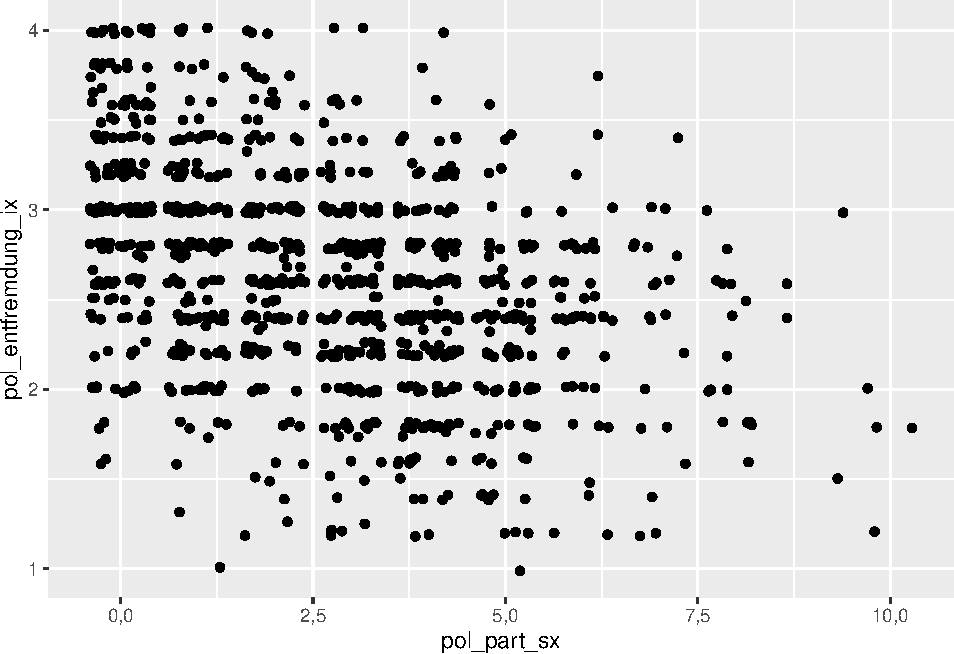
\includegraphics{r_book_files/figure-latex/unnamed-chunk-47-1.pdf}

Betrachtet man den Output, kann man die Beziehung zwischen den beiden Variablen schon erahnen. Es ist zwar keine klare Linie ersichtlich (das wäre auch sehr viel verlangt), aber man kann schon sehen, dass in der Tendenz hohe Werte von politischer Entfremdung mit niedrigen Werten von politischer Partizipation einhergehen und umgekehrt. Die Grafik spricht also für den vermuteten negativen Zusammenhang.

\hypertarget{kovarianz}{%
\subsection{Kovarianz}\label{kovarianz}}

Die Kovarianz ist die gemeinsame Variation der beiden Variablen, beziehungsweise das Produkt der Abweichung beider Variablen von ihrem jeweiligen Mittelwert geteilt durch die Fallzahl. In R kann man die Kovarianz einfach über den Befehl \texttt{cov()} ausgeben lassen (Teil des \texttt{stats}-Paketes, wird üblicherweise mit base R geladen). Die Funktion benötigt im Idealfall lediglich die beiden Variablen/Vektoren, deren Kovarianz ermittelt werden soll. Falls es im Datensatz fehlende Werte gibt braucht es noch einen Hinweis darauf, wie mit diesen umgegangen werden soll (siehe unten Argument \texttt{use}).

\begin{Shaded}
\begin{Highlighting}[]
\FunctionTok{cov}\NormalTok{(df}\SpecialCharTok{$}\NormalTok{pol\_part\_sx, df}\SpecialCharTok{$}\NormalTok{pol\_entfremdung\_ix)}
\end{Highlighting}
\end{Shaded}

\begin{verbatim}
## [1] -0,4992269
\end{verbatim}

Im Beispiel ist die Kovarianz also \text{-0,5}. Das ist insofern gut, weil das Vorzeichen der Prognose aus der Hypothese entspricht. Allerdings können wir noch keine Aussage über die Stärke des Zusammenhangs machen, weil die Kovarianz ein unstandardisiertes Maß für die gemeinsame Variation der beiden Variablen ist. Sie berücksichtigt die Skalierung der Variablen nicht.

\hypertarget{korrelation-mit-base-rstats}{%
\subsection{\texorpdfstring{Korrelation mit \texttt{base\ R}/\texttt{stats}}{Korrelation mit base R/stats}}\label{korrelation-mit-base-rstats}}

Der Korrelationskoeffizient \emph{r} (auch Pearson´s r oder Produkt-Moment-Korrelation) berücksichtigt die Skalierung, weil er die Standardabweichungen der beiden Variablen mit einbezieht. Er beschreibt die Beziehung zwischen zwei metrischen Variablen in einem Wertebereich von -1 über 0 bis +1. Der Wert +1 steht dabei für eine perfekt positive und -1 für eine perfekt negative Beziehung.

Auch der Korrelationskoeffizient lässt sich leicht mit dem \texttt{stats}-Paket berechnen:

\begin{Shaded}
\begin{Highlighting}[]
\FunctionTok{cor}\NormalTok{(df}\SpecialCharTok{$}\NormalTok{pol\_part\_sx, df}\SpecialCharTok{$}\NormalTok{pol\_entfremdung\_ix)}
\end{Highlighting}
\end{Shaded}

\begin{verbatim}
## [1] -0,3998827
\end{verbatim}

Das Vorzeichen bleibt, verglichen mit der Kovarianz, selbstverständlich dasselbe. Die Höhe des Betrags wird jedoch in einen Bereich zwischen 0 und 1 ``gepresst''. Für unsere beiden Variablen ergibt sich eine mittlere Effektstärke von \emph{r} = \text{-0,4}.

Mit einem Signifikanztest, bei dem ein p-Wert berechnet wird, kann man außerdem prüfen, ob ein Korrelationskoeffizient sich signifikant von 0 unterscheidet (Inferenzstatistik). Die Funktion für den Signifikanztest lautet \texttt{cor.test()}. Neben den beiden Variablen kann man der Funktion weitere Argumente mitgeben:

\begin{itemize}
\item
  Das Argument \texttt{use} bestimmt darüber, wie mit fehlenden Werten umgegangen werden soll. Es ist eigentlich nur dann relevant, wenn mehr als zwei Variablen korreliert werden sollen. Dann kann man darüber entscheiden, ob ein Fall für alle mögliche Korrelationen ausgeschlossen werden soll, wenn er bei einer Variable einen fehlenden Wert hat (listenweiser Fallausschluss) oder ob dieser Fall nur bei den Korrelationen ausgeschlossen werden soll, bei denen die Variable beteiligt ist (paarweiser Fallausschluss).
\item
  Im Argument \texttt{alternative} kann man festlegen, um was für eine Alternativhypothese es sich handelt. Hiernach bestimmt sich, in welche \emph{Richtung} der Signifikanztest durchgeführt werden soll und ob \emph{einseitig} oder \emph{zweiseitig} getestet werden soll. Man kann hier die Option \texttt{two.sided} für einen zweiseitigen Test festlegen, wenn man eine ungerichtete Hypothese aufgestellt hat. Für gerichtete Hypothesen stehen die Optionen \texttt{greater} (für positive Zusammenhänge) und \texttt{less} (für negative Zusammenhänge) zur Verfügung.
\item
  Mit dem Argument \texttt{method} kann man auch noch andere Korrelationskoeffizienten als die Pearson-Korrelation berchenen: Für Kendall \texttt{method\ =\ "kendall"} und für Spearman \texttt{method\ =\ "spearman"}.
\end{itemize}

\begin{Shaded}
\begin{Highlighting}[]
\FunctionTok{cor.test}\NormalTok{(df}\SpecialCharTok{$}\NormalTok{pol\_part\_sx, df}\SpecialCharTok{$}\NormalTok{pol\_entfremdung\_ix, }
         \AttributeTok{use =} \StringTok{"complete.obs"}\NormalTok{,}
         \AttributeTok{alternative =} \StringTok{"less"}\NormalTok{)}
\end{Highlighting}
\end{Shaded}

\begin{verbatim}
## 
##  Pearson's product-moment correlation
## 
## data:  df$pol_part_sx and df$pol_entfremdung_ix
## t = -13,803, df = 1001, p-value < 2,2e-16
## alternative hypothesis: true correlation is less than 0
## 95 percent confidence interval:
##  -1,0000000 -0,3552982
## sample estimates:
##        cor 
## -0,3998827
\end{verbatim}

Das Ergebnis ist ein kurzer ``Bericht'' über den Signifikanztest. Angegeben sind z.B. der p-Wert, das Konfidenzintervall und noch einmal der Korrelationskoeffizient. Aus dem p-Wert, der im Beispiel einen sehr niedrigen Wert (kleiner als die geforderten .05) aufweist, können wir schließen, dass der Wert \emph{r} = \text{-0,3998827} signifikant von 0 abweicht, also mit einiger Wahrscheinlichkeit nicht zufällig zustande gekommen ist. Das spricht für unsere Hypothese und damit für die Existenz des vermuteten Zusammenhangs in der Grundgesamtheit. Wir können die Hypothese somit als durch die Daten bestätigt ansehen.

\hypertarget{korrelation-mit-psych}{%
\subsection{\texorpdfstring{Korrelation mit \texttt{psych}}{Korrelation mit psych}}\label{korrelation-mit-psych}}

Den Korrelationskoeffizient kann man in R auch mit vielen anderen Paketen ausrechnen. Beispielhaft soll hier noch der Code für die Korrelation mit dem \texttt{psych}-Paket veranschaulicht werden. Dieses Paket benutzen wir ja auch für viele andere statistische Verfahren und man kann \texttt{psych} mit der Pipe benutzen (tidyverse-Schreibweise). Der Output für die Korrelation sieht leicht anders aus.

Die Funktion für die Korrelation in \texttt{psych} lautet \texttt{corr()} (mit 2 r). Sie benötigt als erstes Argument den Datensatz mit ausschließlich den Variablen, die korreliert werden sollen. Diese können direkt vor der Funktion mit einem \texttt{select()}- Befehl ausgewählt werden. Neben dem Datenobjekt kann man weitere Argumente angeben, z.B. über \texttt{use} den listen- oder paarweisen Fallausschluss und über \texttt{method} die Art der Korrelation. Neben dem standardmäßig eingestellten Wert \texttt{pearson} für den Korrelationskoeffizienten (Pearson´s r) gibt es nämlich noch weitere Maßzahlen für spezielle Daten (z.B. \texttt{spearman} für Rangdaten oder \texttt{kendall} für ordinale Daten).

\begin{Shaded}
\begin{Highlighting}[]
\NormalTok{df }\SpecialCharTok{\%\textgreater{}\%}
  \FunctionTok{select}\NormalTok{(pol\_part\_sx, pol\_entfremdung\_ix) }\SpecialCharTok{\%\textgreater{}\%} 
\NormalTok{  psych}\SpecialCharTok{::}\FunctionTok{corr.test}\NormalTok{(}\AttributeTok{use=}\StringTok{"pairwise"}\NormalTok{, }\AttributeTok{method=}\StringTok{"pearson"}\NormalTok{)}
\end{Highlighting}
\end{Shaded}

\begin{verbatim}
## Call:psych::corr.test(x = ., use = "pairwise", method = "pearson")
## Correlation matrix 
##                    pol_part_sx pol_entfremdung_ix
## pol_part_sx                1,0               -0,4
## pol_entfremdung_ix        -0,4                1,0
## Sample Size 
## [1] 1003
## Probability values (Entries above the diagonal are adjusted for multiple tests.) 
##                    pol_part_sx pol_entfremdung_ix
## pol_part_sx                  0                  0
## pol_entfremdung_ix           0                  0
## 
##  To see confidence intervals of the correlations, print with the short=FALSE option
\end{verbatim}

Der Output sieht leicht anders aus als der oben dargestellte aus dem \texttt{stats}-Paket. Er hat drei wichtige Bereiche:

\begin{itemize}
\item
  Eine Matrix für die Korrelationskoeffizienten. Hier wird die Korrelation jeder Variablen mit jeder anderen im Datensatz dargestellt. In unserem Fall sind das ja nur zwei. Aber mit der Funktion könnten sie auch drei oder noch mehr Variablen miteinander korrelieren. -- Jeweils natürlich nur paarweise. In dieser Matrix ist jede Korrelation doppelt enthalten: Einmal über und einmal unter der mittleren Diagonalen. Das liegt daran, dass die Korrelation zweimal berechnet wird: Zunächst mit der ersten Variable an erster und der zweiten an zweiter Stelle. Danach wird die Position der Variablen getauscht. Für Pearson´s r macht es jedoch keinen Unterschied, welche Reihenfolge die Variablen haben. Deshalb steht dort zweimal die gleiche Zahl. In der Diagonalen finden Sie die Korrelation einer Variablen mit sich selbst. Sie ist logischerweise jeweils = 1, also ein perfekter positiver Zusammenhang.
\item
  Der zweite Bereich gibt Aufschluss über die Sample-Größe. Er wird auch manchmal als Matrix dargestellt, nämlich dann, wenn die Fallzahl für die einzelnen Korrelationen unterschiedlich wäre. Das ist hier aber nicht der Fall.
\item
  Der dritte wichtige Bereich beinhaltet die p-Werte der Korrelationen. Im Beispiel sind alle p-Werte ausgesprochen niedrig, deshalb wird hier ``0'' dargestellt. Das ist natürlich der Rundung geschuldet, denn selbstverständlich ist der p-Wert nie exakt ``0'', da es sich um eine Wahrscheinlichkeit handelt. Er nähert sich lediglich dem Wert 0 an.
\end{itemize}

\hypertarget{partialkorrelation}{%
\subsection{Partialkorrelation}\label{partialkorrelation}}

Bei der Partialkorrelation wird der Einfluss einer dritten Variable aus der Korrelation zwischen zwei Variablen herausgerechnet. Das geschieht über die Residuen (vgl. zukünftiges Kapitel zur Regression/SDA2). Im \texttt{psych}-Paket kann man die Partialkorrelation einfach berechnen. Zur besseren Übersichtlichkeit kann man vorab im \texttt{select()}-Befehl die Variablen auf eine spezielle Weise gruppieren (das kann man aber auch weglassen, dann muss man sich aber merken, welche Variable die Einflussvariable war). Im Anschluss erfolgt die Partialkorrelation durch die Funktion \texttt{partial.r()} und dann durch die Funktion \texttt{corr.p()} der entsprechende Signifikanztest:

\begin{Shaded}
\begin{Highlighting}[]
\NormalTok{df }\SpecialCharTok{\%\textgreater{}\%} 
  \FunctionTok{select}\NormalTok{(}\AttributeTok{x =} \FunctionTok{c}\NormalTok{(pol\_part\_sx, pol\_entfremdung\_ix), }\AttributeTok{y =}\NormalTok{ alter) }\SpecialCharTok{\%\textgreater{}\%} 
\NormalTok{  psych}\SpecialCharTok{::}\FunctionTok{partial.r}\NormalTok{() }\SpecialCharTok{\%\textgreater{}\%} 
\NormalTok{  psych}\SpecialCharTok{::}\FunctionTok{corr.p}\NormalTok{(}\AttributeTok{n =}\DecValTok{1003}\NormalTok{)}
\end{Highlighting}
\end{Shaded}

\begin{verbatim}
## Call:psych::corr.p(r = ., n = 1003)
## Correlation matrix 
##       x1    x2     y
## x1  1,00 -0,38  0,22
## x2 -0,38  1,00 -0,05
## y   0,22 -0,05  1,00
## Sample Size 
## [1] 1003
## Probability values (Entries above the diagonal are adjusted for multiple tests.) 
##    x1   x2    y
## x1  0 0,00 0,00
## x2  0 0,00 0,15
## y   0 0,15 0,00
## 
##  To see confidence intervals of the correlations, print with the short=FALSE option
\end{verbatim}

Der Output sieht ähnlich aus wie zuvor, nur dass in den Zellen jetzt jeweils die Korrelation zwischen zwei Variablen dargestellt ist, bereinigt um die jeweils dritte. Für die uns interessierende Korrelation zwischen politischer Partizipation und politischer Entfremdung ist der Korrelationskoeffizient hier nur leicht gesunken. Er beträgt jetzt noch \emph{r-partial} = \text{-0,38}. Der Einfluss des Alters auf unseren Zusammenhang war also vermutlich nicht besonders stark. Auch nach Kontrolle dieser Drittvariable hat unsere Alternativhypothese also Bestand.

Man kann sogar in der Korrelations-Matrix oben sehen, dass das Alter lediglich mit der Variable \emph{politische Partizipation} einen Zusammenhang hat, aber kaum mit \emph{politischer Entfremdung}. Vermutlich wird ein Teil der Varianz in der politischen Partizipation durch das Alter erklärt. Dass diese Variablen ebenfalls kovariieren, macht inhaltlich sogar Sinn: Wer älter ist, hatte bereits mehr Gelegenheit zur politischen Partizipation und einige Partizipationsmöglichkeiten kann man sogar erst mit einem gewissen Alter ausüben, wie beispielsweise das Wählen.

\hypertarget{korrelationsmatrizen-darstellen}{%
\subsection{Korrelationsmatrizen darstellen}\label{korrelationsmatrizen-darstellen}}

Zum Abschluss dieses Teils möchte ich noch kurz darauf eingehen, dass man natürlich auch mehrere oder sogar viele Korrelationen in einer Matrix darstellen kann. R liefert sogar ganz schöne Grafiken, die Zusammenhänge zwischen metrischen Variablen übersichtlich darstellen können. Ein Paket, welches dazu benutzt werden kann, ist \texttt{corrr}.

Ich greife im Folgenden auf einen anderen Datensatz zu, nämlich auf den Datensatz \texttt{mtcars} aus dem tidyverse. In dem Datensatz sind Statistiken über verschiedene Automodelle gesammelt, aber der Inhalt ist an dieser Stelle nicht so wichtig.

Die Funktion \texttt{correlate()} aus dem \texttt{corrr}-Paket liefert zunächst die Korrelationsmatrix der Daten. Signifikanztests liefert das Paket nicht, denn es ist eher für die explorative Vorgehensweise geeignet (= nicht inferenzstatistisch-Hypothesenprüfend).

\begin{Shaded}
\begin{Highlighting}[]
\NormalTok{mtcars }\SpecialCharTok{\%\textgreater{}\%} 
\NormalTok{  corrr}\SpecialCharTok{::}\FunctionTok{correlate}\NormalTok{() }
\end{Highlighting}
\end{Shaded}

\begin{verbatim}
## 
## Correlation method: 'pearson'
## Missing treated using: 'pairwise.complete.obs'
\end{verbatim}

\begin{verbatim}
## # A tibble: 11 x 12
##    term     mpg    cyl   disp     hp    drat     wt    qsec     vs      am
##    <chr>  <dbl>  <dbl>  <dbl>  <dbl>   <dbl>  <dbl>   <dbl>  <dbl>   <dbl>
##  1 mpg   NA     -0.852 -0.848 -0.776  0.681  -0.868  0.419   0.664  0.600 
##  2 cyl   -0.852 NA      0.902  0.832 -0.700   0.782 -0.591  -0.811 -0.523 
##  3 disp  -0.848  0.902 NA      0.791 -0.710   0.888 -0.434  -0.710 -0.591 
##  4 hp    -0.776  0.832  0.791 NA     -0.449   0.659 -0.708  -0.723 -0.243 
##  5 drat   0.681 -0.700 -0.710 -0.449 NA      -0.712  0.0912  0.440  0.713 
##  6 wt    -0.868  0.782  0.888  0.659 -0.712  NA     -0.175  -0.555 -0.692 
##  7 qsec   0.419 -0.591 -0.434 -0.708  0.0912 -0.175 NA       0.745 -0.230 
##  8 vs     0.664 -0.811 -0.710 -0.723  0.440  -0.555  0.745  NA      0.168 
##  9 am     0.600 -0.523 -0.591 -0.243  0.713  -0.692 -0.230   0.168 NA     
## 10 gear   0.480 -0.493 -0.556 -0.126  0.700  -0.583 -0.213   0.206  0.794 
## 11 carb  -0.551  0.527  0.395  0.750 -0.0908  0.428 -0.656  -0.570  0.0575
## # ... with 2 more variables: gear <dbl>, carb <dbl>
\end{verbatim}

Mit der Funktion \texttt{rplot()} kann man die Matrix in eine Korrelations-Grafik überführen:

\begin{Shaded}
\begin{Highlighting}[]
\NormalTok{mtcars }\SpecialCharTok{\%\textgreater{}\%} 
\NormalTok{  corrr}\SpecialCharTok{::}\FunctionTok{correlate}\NormalTok{() }\SpecialCharTok{\%\textgreater{}\%}
\NormalTok{  corrr}\SpecialCharTok{::}\FunctionTok{rplot}\NormalTok{()}
\end{Highlighting}
\end{Shaded}

\begin{verbatim}
## 
## Correlation method: 'pearson'
## Missing treated using: 'pairwise.complete.obs'
\end{verbatim}

\begin{verbatim}
## Don't know how to automatically pick scale for object of type noquote. Defaulting to continuous.
\end{verbatim}

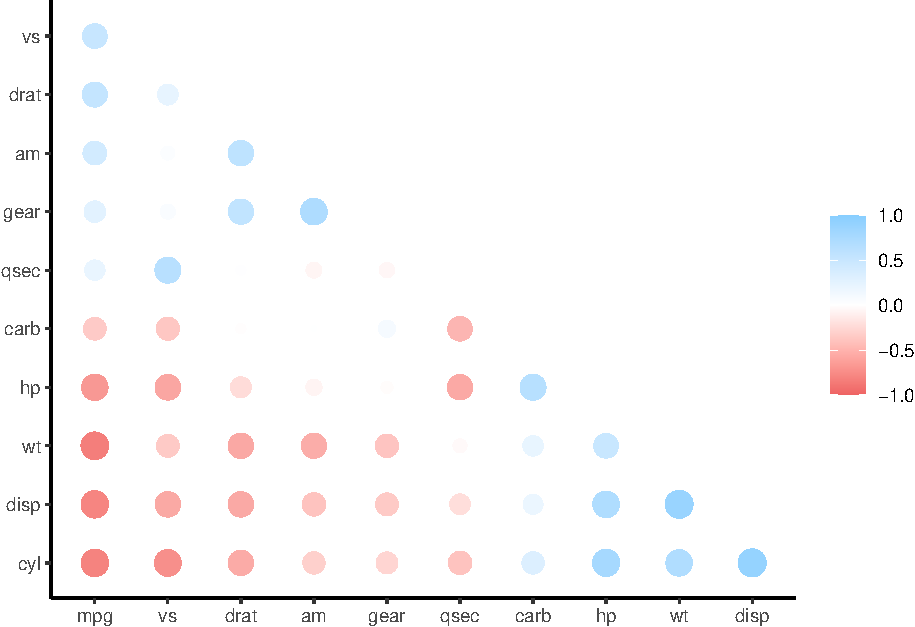
\includegraphics{r_book_files/figure-latex/unnamed-chunk-55-1.pdf}

Das Paket liefert außerdem weitere Funktionen, die dabei helfen, die Matrix und damit auch die Grafik schöner zu formatieren. Mit \texttt{rearrange()} kann man die Variablen in der Matrix nach der Größe der Korrelation sortieren. Mit \texttt{shave} kann man die ``doppelte'' obere Hälfte des Plots abschneiden.

\begin{Shaded}
\begin{Highlighting}[]
\NormalTok{mtcars }\SpecialCharTok{\%\textgreater{}\%} 
\NormalTok{  corrr}\SpecialCharTok{::}\FunctionTok{correlate}\NormalTok{() }\SpecialCharTok{\%\textgreater{}\%}
\NormalTok{  corrr}\SpecialCharTok{::}\FunctionTok{rearrange}\NormalTok{() }\SpecialCharTok{\%\textgreater{}\%}
\NormalTok{  corrr}\SpecialCharTok{::}\FunctionTok{shave}\NormalTok{() }\SpecialCharTok{\%\textgreater{}\%} 
\NormalTok{  corrr}\SpecialCharTok{::}\FunctionTok{rplot}\NormalTok{()}
\end{Highlighting}
\end{Shaded}

\begin{verbatim}
## 
## Correlation method: 'pearson'
## Missing treated using: 'pairwise.complete.obs'
\end{verbatim}

\begin{verbatim}
## Registered S3 methods overwritten by 'registry':
##   method               from 
##   print.registry_field proxy
##   print.registry_entry proxy
\end{verbatim}

\begin{verbatim}
## Don't know how to automatically pick scale for object of type noquote. Defaulting to continuous.
\end{verbatim}

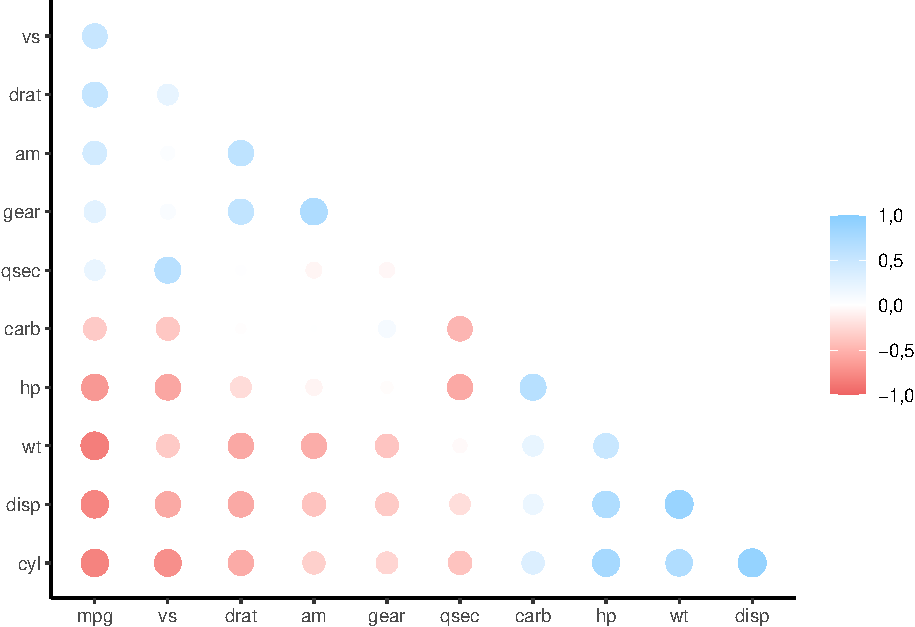
\includegraphics{r_book_files/figure-latex/unnamed-chunk-56-1.pdf}

Sehr schön übersichtlich. Welche Variablen hier wie zusammenhängen, sieht man auf den ersten Blick!

\hypertarget{wichtige-funktionen-aus-diesem-kapitel-3}{%
\section*{Wichtige Funktionen aus diesem Kapitel}\label{wichtige-funktionen-aus-diesem-kapitel-3}}
\addcontentsline{toc}{section}{Wichtige Funktionen aus diesem Kapitel}

\begin{longtable}[]{@{}llll@{}}
\toprule
\begin{minipage}[b]{(\columnwidth - 3\tabcolsep) * \real{0.22}}\raggedright
Funktion\strut
\end{minipage} & \begin{minipage}[b]{(\columnwidth - 3\tabcolsep) * \real{0.16}}\raggedright
Paket\strut
\end{minipage} & \begin{minipage}[b]{(\columnwidth - 3\tabcolsep) * \real{0.37}}\raggedright
Beschreibung\strut
\end{minipage} & \begin{minipage}[b]{(\columnwidth - 3\tabcolsep) * \real{0.26}}\raggedright
Wichtige Argumente/Bemerkung\strut
\end{minipage}\tabularnewline
\midrule
\endhead
\begin{minipage}[t]{(\columnwidth - 3\tabcolsep) * \real{0.22}}\raggedright
\textbf{Tabellenanalyse}\strut
\end{minipage} & \begin{minipage}[t]{(\columnwidth - 3\tabcolsep) * \real{0.16}}\raggedright
\strut
\end{minipage} & \begin{minipage}[t]{(\columnwidth - 3\tabcolsep) * \real{0.37}}\raggedright
\strut
\end{minipage} & \begin{minipage}[t]{(\columnwidth - 3\tabcolsep) * \real{0.26}}\raggedright
\strut
\end{minipage}\tabularnewline
\begin{minipage}[t]{(\columnwidth - 3\tabcolsep) * \real{0.22}}\raggedright
\texttt{tabyl()}\strut
\end{minipage} & \begin{minipage}[t]{(\columnwidth - 3\tabcolsep) * \real{0.16}}\raggedright
janitor\strut
\end{minipage} & \begin{minipage}[t]{(\columnwidth - 3\tabcolsep) * \real{0.37}}\raggedright
Tabellen \& Kreuztabellen\strut
\end{minipage} & \begin{minipage}[t]{(\columnwidth - 3\tabcolsep) * \real{0.26}}\raggedright
\texttt{show\_na\ =\ FALSE}\strut
\end{minipage}\tabularnewline
\begin{minipage}[t]{(\columnwidth - 3\tabcolsep) * \real{0.22}}\raggedright
\texttt{adorn\_totals()}\strut
\end{minipage} & \begin{minipage}[t]{(\columnwidth - 3\tabcolsep) * \real{0.16}}\raggedright
janitor\strut
\end{minipage} & \begin{minipage}[t]{(\columnwidth - 3\tabcolsep) * \real{0.37}}\raggedright
Randhäufigkeiten hinzufügen\strut
\end{minipage} & \begin{minipage}[t]{(\columnwidth - 3\tabcolsep) * \real{0.26}}\raggedright
\texttt{where\ =\ c("row",\ "col")}\strut
\end{minipage}\tabularnewline
\begin{minipage}[t]{(\columnwidth - 3\tabcolsep) * \real{0.22}}\raggedright
\texttt{adorn\_percentages}\strut
\end{minipage} & \begin{minipage}[t]{(\columnwidth - 3\tabcolsep) * \real{0.16}}\raggedright
janitor\strut
\end{minipage} & \begin{minipage}[t]{(\columnwidth - 3\tabcolsep) * \real{0.37}}\raggedright
In Prozentwerte umwandeln\strut
\end{minipage} & \begin{minipage}[t]{(\columnwidth - 3\tabcolsep) * \real{0.26}}\raggedright
\texttt{denominator\ =\ "col"}\strut
\end{minipage}\tabularnewline
\begin{minipage}[t]{(\columnwidth - 3\tabcolsep) * \real{0.22}}\raggedright
\texttt{adorn\_pct\_formatting}\strut
\end{minipage} & \begin{minipage}[t]{(\columnwidth - 3\tabcolsep) * \real{0.16}}\raggedright
janitor\strut
\end{minipage} & \begin{minipage}[t]{(\columnwidth - 3\tabcolsep) * \real{0.37}}\raggedright
Formatierung der Prozentwerte\strut
\end{minipage} & \begin{minipage}[t]{(\columnwidth - 3\tabcolsep) * \real{0.26}}\raggedright
\texttt{digits\ =\ n}\strut
\end{minipage}\tabularnewline
\begin{minipage}[t]{(\columnwidth - 3\tabcolsep) * \real{0.22}}\raggedright
\texttt{adorn\_ns()}\strut
\end{minipage} & \begin{minipage}[t]{(\columnwidth - 3\tabcolsep) * \real{0.16}}\raggedright
janitor\strut
\end{minipage} & \begin{minipage}[t]{(\columnwidth - 3\tabcolsep) * \real{0.37}}\raggedright
Absolute Häufigkeiten wieder hinzufügen\strut
\end{minipage} & \begin{minipage}[t]{(\columnwidth - 3\tabcolsep) * \real{0.26}}\raggedright
\strut
\end{minipage}\tabularnewline
\begin{minipage}[t]{(\columnwidth - 3\tabcolsep) * \real{0.22}}\raggedright
\texttt{adorn\_titel()}\strut
\end{minipage} & \begin{minipage}[t]{(\columnwidth - 3\tabcolsep) * \real{0.16}}\raggedright
janitor\strut
\end{minipage} & \begin{minipage}[t]{(\columnwidth - 3\tabcolsep) * \real{0.37}}\raggedright
Variablen in die erste Zelle schreiben\strut
\end{minipage} & \begin{minipage}[t]{(\columnwidth - 3\tabcolsep) * \real{0.26}}\raggedright
\texttt{placement\ =\ "combined"}\strut
\end{minipage}\tabularnewline
\begin{minipage}[t]{(\columnwidth - 3\tabcolsep) * \real{0.22}}\raggedright
\texttt{chisq.test()}\strut
\end{minipage} & \begin{minipage}[t]{(\columnwidth - 3\tabcolsep) * \real{0.16}}\raggedright
janitor\strut
\end{minipage} & \begin{minipage}[t]{(\columnwidth - 3\tabcolsep) * \real{0.37}}\raggedright
Chi-Quadrat-Test\strut
\end{minipage} & \begin{minipage}[t]{(\columnwidth - 3\tabcolsep) * \real{0.26}}\raggedright
einfache Kreuztabelle\strut
\end{minipage}\tabularnewline
\begin{minipage}[t]{(\columnwidth - 3\tabcolsep) * \real{0.22}}\raggedright
\texttt{CramerV()}\strut
\end{minipage} & \begin{minipage}[t]{(\columnwidth - 3\tabcolsep) * \real{0.16}}\raggedright
DescTools\strut
\end{minipage} & \begin{minipage}[t]{(\columnwidth - 3\tabcolsep) * \real{0.37}}\raggedright
Cramer´s V\strut
\end{minipage} & \begin{minipage}[t]{(\columnwidth - 3\tabcolsep) * \real{0.26}}\raggedright
Kreuztabelle ohne erste Spalte!\strut
\end{minipage}\tabularnewline
\begin{minipage}[t]{(\columnwidth - 3\tabcolsep) * \real{0.22}}\raggedright
\textbf{Kovarianz \& Korrelation}\strut
\end{minipage} & \begin{minipage}[t]{(\columnwidth - 3\tabcolsep) * \real{0.16}}\raggedright
\strut
\end{minipage} & \begin{minipage}[t]{(\columnwidth - 3\tabcolsep) * \real{0.37}}\raggedright
\strut
\end{minipage} & \begin{minipage}[t]{(\columnwidth - 3\tabcolsep) * \real{0.26}}\raggedright
\strut
\end{minipage}\tabularnewline
\begin{minipage}[t]{(\columnwidth - 3\tabcolsep) * \real{0.22}}\raggedright
\texttt{cov()}\strut
\end{minipage} & \begin{minipage}[t]{(\columnwidth - 3\tabcolsep) * \real{0.16}}\raggedright
stats\strut
\end{minipage} & \begin{minipage}[t]{(\columnwidth - 3\tabcolsep) * \real{0.37}}\raggedright
Kovarianz\strut
\end{minipage} & \begin{minipage}[t]{(\columnwidth - 3\tabcolsep) * \real{0.26}}\raggedright
\strut
\end{minipage}\tabularnewline
\begin{minipage}[t]{(\columnwidth - 3\tabcolsep) * \real{0.22}}\raggedright
\texttt{cor()}\strut
\end{minipage} & \begin{minipage}[t]{(\columnwidth - 3\tabcolsep) * \real{0.16}}\raggedright
stats\strut
\end{minipage} & \begin{minipage}[t]{(\columnwidth - 3\tabcolsep) * \real{0.37}}\raggedright
Korrelation\strut
\end{minipage} & \begin{minipage}[t]{(\columnwidth - 3\tabcolsep) * \real{0.26}}\raggedright
\strut
\end{minipage}\tabularnewline
\begin{minipage}[t]{(\columnwidth - 3\tabcolsep) * \real{0.22}}\raggedright
\texttt{cor.test()}\strut
\end{minipage} & \begin{minipage}[t]{(\columnwidth - 3\tabcolsep) * \real{0.16}}\raggedright
stats\strut
\end{minipage} & \begin{minipage}[t]{(\columnwidth - 3\tabcolsep) * \real{0.37}}\raggedright
Signifikanztest für r\strut
\end{minipage} & \begin{minipage}[t]{(\columnwidth - 3\tabcolsep) * \real{0.26}}\raggedright
\texttt{use}, \texttt{alternative}\strut
\end{minipage}\tabularnewline
\begin{minipage}[t]{(\columnwidth - 3\tabcolsep) * \real{0.22}}\raggedright
\texttt{corr.test()}\strut
\end{minipage} & \begin{minipage}[t]{(\columnwidth - 3\tabcolsep) * \real{0.16}}\raggedright
psych\strut
\end{minipage} & \begin{minipage}[t]{(\columnwidth - 3\tabcolsep) * \real{0.37}}\raggedright
Korrelation + Signifikanztest\strut
\end{minipage} & \begin{minipage}[t]{(\columnwidth - 3\tabcolsep) * \real{0.26}}\raggedright
\texttt{use}, \texttt{method}\strut
\end{minipage}\tabularnewline
\begin{minipage}[t]{(\columnwidth - 3\tabcolsep) * \real{0.22}}\raggedright
\texttt{partial.r()}\strut
\end{minipage} & \begin{minipage}[t]{(\columnwidth - 3\tabcolsep) * \real{0.16}}\raggedright
psych\strut
\end{minipage} & \begin{minipage}[t]{(\columnwidth - 3\tabcolsep) * \real{0.37}}\raggedright
Partialkorrelation\strut
\end{minipage} & \begin{minipage}[t]{(\columnwidth - 3\tabcolsep) * \real{0.26}}\raggedright
\strut
\end{minipage}\tabularnewline
\begin{minipage}[t]{(\columnwidth - 3\tabcolsep) * \real{0.22}}\raggedright
\texttt{corr.p()}\strut
\end{minipage} & \begin{minipage}[t]{(\columnwidth - 3\tabcolsep) * \real{0.16}}\raggedright
psych\strut
\end{minipage} & \begin{minipage}[t]{(\columnwidth - 3\tabcolsep) * \real{0.37}}\raggedright
Signifikanztest für Partialkorrelation\strut
\end{minipage} & \begin{minipage}[t]{(\columnwidth - 3\tabcolsep) * \real{0.26}}\raggedright
\texttt{n}\strut
\end{minipage}\tabularnewline
\begin{minipage}[t]{(\columnwidth - 3\tabcolsep) * \real{0.22}}\raggedright
\texttt{correlate()}\strut
\end{minipage} & \begin{minipage}[t]{(\columnwidth - 3\tabcolsep) * \real{0.16}}\raggedright
corrr\strut
\end{minipage} & \begin{minipage}[t]{(\columnwidth - 3\tabcolsep) * \real{0.37}}\raggedright
Korrelationsmatrix\strut
\end{minipage} & \begin{minipage}[t]{(\columnwidth - 3\tabcolsep) * \real{0.26}}\raggedright
\strut
\end{minipage}\tabularnewline
\begin{minipage}[t]{(\columnwidth - 3\tabcolsep) * \real{0.22}}\raggedright
\textbf{Grafiken}\strut
\end{minipage} & \begin{minipage}[t]{(\columnwidth - 3\tabcolsep) * \real{0.16}}\raggedright
\strut
\end{minipage} & \begin{minipage}[t]{(\columnwidth - 3\tabcolsep) * \real{0.37}}\raggedright
\strut
\end{minipage} & \begin{minipage}[t]{(\columnwidth - 3\tabcolsep) * \real{0.26}}\raggedright
\strut
\end{minipage}\tabularnewline
\begin{minipage}[t]{(\columnwidth - 3\tabcolsep) * \real{0.22}}\raggedright
\texttt{ggplot()}\strut
\end{minipage} & \begin{minipage}[t]{(\columnwidth - 3\tabcolsep) * \real{0.16}}\raggedright
ggplot2\strut
\end{minipage} & \begin{minipage}[t]{(\columnwidth - 3\tabcolsep) * \real{0.37}}\raggedright
Plot anlegen\strut
\end{minipage} & \begin{minipage}[t]{(\columnwidth - 3\tabcolsep) * \real{0.26}}\raggedright
\texttt{aes()}\strut
\end{minipage}\tabularnewline
\begin{minipage}[t]{(\columnwidth - 3\tabcolsep) * \real{0.22}}\raggedright
\texttt{geom\_jitter()}\strut
\end{minipage} & \begin{minipage}[t]{(\columnwidth - 3\tabcolsep) * \real{0.16}}\raggedright
ggplot2\strut
\end{minipage} & \begin{minipage}[t]{(\columnwidth - 3\tabcolsep) * \real{0.37}}\raggedright
``zitternder'' Scatterplot\strut
\end{minipage} & \begin{minipage}[t]{(\columnwidth - 3\tabcolsep) * \real{0.26}}\raggedright
\strut
\end{minipage}\tabularnewline
\begin{minipage}[t]{(\columnwidth - 3\tabcolsep) * \real{0.22}}\raggedright
\texttt{aes()}\strut
\end{minipage} & \begin{minipage}[t]{(\columnwidth - 3\tabcolsep) * \real{0.16}}\raggedright
ggplot2\strut
\end{minipage} & \begin{minipage}[t]{(\columnwidth - 3\tabcolsep) * \real{0.37}}\raggedright
``Ästhetik'' des Plots\strut
\end{minipage} & \begin{minipage}[t]{(\columnwidth - 3\tabcolsep) * \real{0.26}}\raggedright
Variablen, die im Plot darzustellen sind\strut
\end{minipage}\tabularnewline
\begin{minipage}[t]{(\columnwidth - 3\tabcolsep) * \real{0.22}}\raggedright
\texttt{rplot()}\strut
\end{minipage} & \begin{minipage}[t]{(\columnwidth - 3\tabcolsep) * \real{0.16}}\raggedright
corrr\strut
\end{minipage} & \begin{minipage}[t]{(\columnwidth - 3\tabcolsep) * \real{0.37}}\raggedright
Korrelations-Plot\strut
\end{minipage} & \begin{minipage}[t]{(\columnwidth - 3\tabcolsep) * \real{0.26}}\raggedright
\strut
\end{minipage}\tabularnewline
\bottomrule
\end{longtable}

\hypertarget{grafiken}{%
\chapter{Grafiken}\label{grafiken}}

Grafiken erfüllen bei der Datenanalyse zwei sehr wichtige Funktionen: Zum einen dienen Sie der explorativen Analyse und helfen dabei, selbst ein besseres Verständnis für die eigenen Daten zu entwickeln. Zum anderen dienen Grafiken aber auch dazu, die Ergebnisse der eigenen Analyse darzustellen um sie anderen mitzuteilen.

In den vorhergehenden Kapiteln haben wir erste Grafiken bereits kennengelernt (z.B. Balkendiagramme und Streudiagramme). In diesem Kapitel möchte ich aber detaillierter darauf eingehen, wie Grafiken mit R erzeugt werden können. Wie so oft gibt es dazu verschiedene Wege. Auch base-R bietet einige Funktionen, mit denen Grafiken schnell erzeugt und individuell angepasst werden können. Leider ist dieses Anpassen in base-R für R-Anfänger gar nicht so einfach. Da das Anpassen einer Grafik aber nahezu immer nötig ist, gehe ich hier deshalb nicht auf die base-R-Funktionen zum Erzeugen von Grafiken ein.

Selbstverständlich gibt es auch über das tidyverse einen Weg, statistische Grafiken herzustellen. Das entsprechende Paket heißt \texttt{ggplot2}. Es beruht auf der \emph{Grammar of Graphics} (mehr zum Hintergrund finden Sie \href{http://vita.had.co.nz/papers/layered-grammar.pdf}{hier}). Die Idee dahinter ist, dass eine Grafik aus mehreren \emph{Layern} zusammengesetzt ist. Das kann man sich einerseits ein bisschen so wie bei einem Overhead-Projektor (kennen Sie solche Geräte noch?) vorstellen, bei dem man mehrere transparente Folien übereinanderlegt und dann ein gemeinsames Bild erzeugt -- oder wie die Ebenen bei Photoshop. Andererseits sind Layer auch die „Stellschrauben`` mit denen man am Aussehen einer Grafik drehen kann.

Das Paket \texttt{ggplot2} ist sehr sensibel, was die Daten angeht, die als Input für die Grafiken dienen. Diese müssen auf jeden Fall \texttt{tidy} sein und bisweilen wird ein \emph{long format} benötigt. Dazu später mehr.

\hypertarget{drei-basis-funktionen}{%
\section{Drei Basis-Funktionen}\label{drei-basis-funktionen}}

Möchte man eine Grafik mit `ggplot2 erzeugen benötigt man mindestens die folgenden drei Funktionen. Aber natürlich kann man jede Grafik noch komplexer machen und umgestalten, wenn man weitere Funktionen hinzufügt.

Die Basis-Funktionen von \texttt{ggplot2} sind:

\texttt{ggplot()}: Diese Funktion ist immer der erste Schritt. Durch die Funktion wird einen sogenanntes \emph{Plot}-Objekt angelegt, also die Grafik an sich. Die Funktion erhält als erstes Argument das Datenobjekt, auf dem die Grafik basieren soll. Zu Beginn ist der Plot leer.

\texttt{aes()}: Mit dieser Hilfsfunktion wird das \emph{aesthetic mapping} definiert. Über das *aesthtic mapping können wir bestimmen, wie Daten/Variablen in Formatierung übersetzt werden sollen.

\texttt{geom\_()}: Es gibt unterschiedliche \texttt{geom\_()}-Funktionen. Ein Geom ist ein \emph{geom}etisches Objekt, dass auf dem Plot platziert werden soll, z.B. ein Balkendiagramm (\texttt{geom\_bar()}) oder eine horizontale Linie (\texttt{geom\_hline()}). Eine statistische Grafik benötigt mindestens ein Geom, kann aber auch mehrere enthalten.

Zusätzlich gibt es in ggplot noch eine Besonderheit: Der Operator \texttt{+} wird in diesem Paket dazu eingesetzt, um die einzelnen grafischen Elemente (oder Layer) zusammenzufügen. Das Pluszeichen steht immer nach einem Befehl, wenn ein Plot noch nicht beendet ist und noch ein weiteres Element hinzugefügt werden soll (so ähnlich wie die Pipe). Das \texttt{+} steht immer am Ende der Zeile, nie am Beginn.

Im Zusammenspiel sieht das so aus (Pseudocode):

\begin{Shaded}
\begin{Highlighting}[]
\FunctionTok{ggplot}\NormalTok{(}\AttributeTok{data =}\NormalTok{ data, }\AttributeTok{mapping =} \FunctionTok{aes}\NormalTok{(}\AttributeTok{x =}\NormalTok{ var\_1)) }\SpecialCharTok{+}
  \FunctionTok{geom\_bar}\NormalTok{()}
\end{Highlighting}
\end{Shaded}

In tidyverse-Schreibweise auch so:

\begin{Shaded}
\begin{Highlighting}[]
\NormalTok{data }\SpecialCharTok{\%\textgreater{}\%} 
  \FunctionTok{ggplot}\NormalTok{(}\AttributeTok{mapping =} \FunctionTok{aes}\NormalTok{(}\AttributeTok{x =}\NormalTok{ var\_1)) }\SpecialCharTok{+}
  \FunctionTok{geom\_bar}\NormalTok{()}
\end{Highlighting}
\end{Shaded}

Und verkürzt kann man die Namen der Argumente weglassen. Routinierte R-Anwender tun dies häufig, deshalb sollten Sie das mal gesehen haben:

\begin{Shaded}
\begin{Highlighting}[]
\NormalTok{data }\SpecialCharTok{\%\textgreater{}\%} 
  \FunctionTok{ggplot}\NormalTok{(}\FunctionTok{aes}\NormalTok{(var\_1)) }\SpecialCharTok{+}
  \FunctionTok{geom\_bar}\NormalTok{()}
\end{Highlighting}
\end{Shaded}

Um explizit zu machen, was jeweils passiert, werden wir hier aber die ausführliche Schreibweise nutzen.

Im Folgenden wollen wir uns natürlich ein paar Grafiken und Formatierungsmöglichkeiten anschauen. Allerdings ist \texttt{ggplot} so umfangreich, dass wir die Funktionen nicht annähernd durchgehen können. Für dieses Kapitel gilt daher im besonderen Maß: Wenn Sie eine Formatierung vornehmen möchten, die hier nicht angesprochen wird, googeln Sie danach! Die Möglichkeiten der Gestaltung mit \texttt{ggplot2} sind schier unendlich.

Als Datenbeispiel benutzen wir auch in diesem Kapitel den Generation Z-Datensatz. Die erste Grafik, die wir hier erstellen wollen, thematisiert die politische Partizipation der Befragten und zwar getrennt für Jugendliche und junge Erwachsene. Ich werde anhand von diesem Beispiel auch noch einmal den Einsatz der drei „Basis-Funktionen`` beschreiben.

\hypertarget{erste-funktion-plot-objekt-erstellen}{%
\section{Erste Funktion: Plot-Objekt erstellen}\label{erste-funktion-plot-objekt-erstellen}}

Jede \texttt{ggplot2}-Grafik beginnt immer mit dieser Funktion und der Übergabe von einem Datenobjekt als erstem Argument. Dabei ist es egal, ob wir die Base-R oder die tidyverse-Schreibweise wählen.

\begin{Shaded}
\begin{Highlighting}[]
\NormalTok{p }\OtherTok{\textless{}{-}}\NormalTok{ df }\SpecialCharTok{\%\textgreater{}\%} 
  \FunctionTok{ggplot}\NormalTok{()}
\end{Highlighting}
\end{Shaded}

\hypertarget{zweite-funktion-aesthetik-mapping}{%
\section{Zweite Funktion: Aesthetik Mapping}\label{zweite-funktion-aesthetik-mapping}}

Die \texttt{ggplot()} kann noch ein zweites Argument haben, nämlich \texttt{mapping\ =}. Über dieses Argument wird das aesthteic mapping festgelegt. Wie bereits beschrieben, betrifft dies die Zuordnung von Daten im Datensatz zum Aussehen der fertigen Grafik. Man muss quasi beschreiben, wie die die Daten in Layout übersetzt werden sollen.

Das Mapping geschieht über die Hilfsfunktion \texttt{aes()}. Diese Funktion benötigt Argumente, damit sie die Formatierung umsetzen kann:

\begin{Shaded}
\begin{Highlighting}[]
\NormalTok{p }\OtherTok{\textless{}{-}}\NormalTok{ df }\SpecialCharTok{\%\textgreater{}\%} 
  \FunctionTok{ggplot}\NormalTok{(}\AttributeTok{mapping =} \FunctionTok{aes}\NormalTok{(}\AttributeTok{x =}\NormalTok{ volljaehrigkeit,}
                       \AttributeTok{y =}\NormalTok{ pol\_part\_sx))}
\end{Highlighting}
\end{Shaded}

\textbf{Zwingende Argumente}

In unserem Beispiel möchten wir die Gruppierungsvariable „Volljährigkeit`` auf der X-Achse darstellen und die metrische Variable „politische Partizipation`` auf der Y-Achse. Die beiden Argumente für die \texttt{aes()} heißen entsprechend x und y. Diese beiden Argumente für die Achsen werden von Geomen häufig vorausgesetzt, damit das entsprechende Geom überhaupt erzeugt werden kann (zwingende Argumente). Einige Geome benötigen aber auch nur das x-Argument (z.B. ganz einfache Häufigkeitsverteilungen von einzelnen Variablen).

\textbf{Optionale Argumente}

Die \texttt{aes()}-Funktion kann zusätzlich zu den zwingenden Argumenten für die Achsen auch optionale Argumente haben. Argumente wie \texttt{fill} (Farbe der Füllung), \texttt{color}, \texttt{size}, \texttt{shape}, \texttt{linetype} oder \texttt{group} kann man dazu benutzen, die Formatierung der Grafik zusätzlich durch Variablen zu verändern.

In unserer Grafik bietet es sich an, die Gruppenzugehörigkeit nicht nur durch die Anordnung der Gruppenvariable auf der X-Achse, sondern zusätzlich noch durch Farbe zu unterstreichen.

\begin{Shaded}
\begin{Highlighting}[]
\NormalTok{p }\OtherTok{\textless{}{-}}\NormalTok{ df }\SpecialCharTok{\%\textgreater{}\%} 
  \FunctionTok{ggplot}\NormalTok{(}\AttributeTok{mapping =} \FunctionTok{aes}\NormalTok{(}\AttributeTok{x =}\NormalTok{ volljaehrigkeit,}
                       \AttributeTok{y =}\NormalTok{ pol\_part\_sx, }
                       \AttributeTok{color =}\NormalTok{ volljaehrigkeit))}
\end{Highlighting}
\end{Shaded}

Das Mapping kann übrigens entweder gleich zu Beginn der Grafik in der Funktion \texttt{ggplot()} passieren, dann gilt es für den gesamten Plot. Oder es steht in einer \texttt{geom\_()}-Funktion (nächster Schritt), dann gilt dieses Mapping nur für das spezifische Geom. Hat man nur ein Geom, ist es egal wo es steht.

\hypertarget{dritte-funktion-geom-hinzufuxfcgen}{%
\section{Dritte Funktion: Geom hinzufügen}\label{dritte-funktion-geom-hinzufuxfcgen}}

Das soeben erzeugte Objekt \texttt{p} ist leer. Zwar existiert schon eine Zuordnung der Daten zu den Achsen, aber eine Grafik wurde bisher nicht erzeugt:

\begin{Shaded}
\begin{Highlighting}[]
\CommentTok{\# plot ausgeben}
\NormalTok{p }
\end{Highlighting}
\end{Shaded}

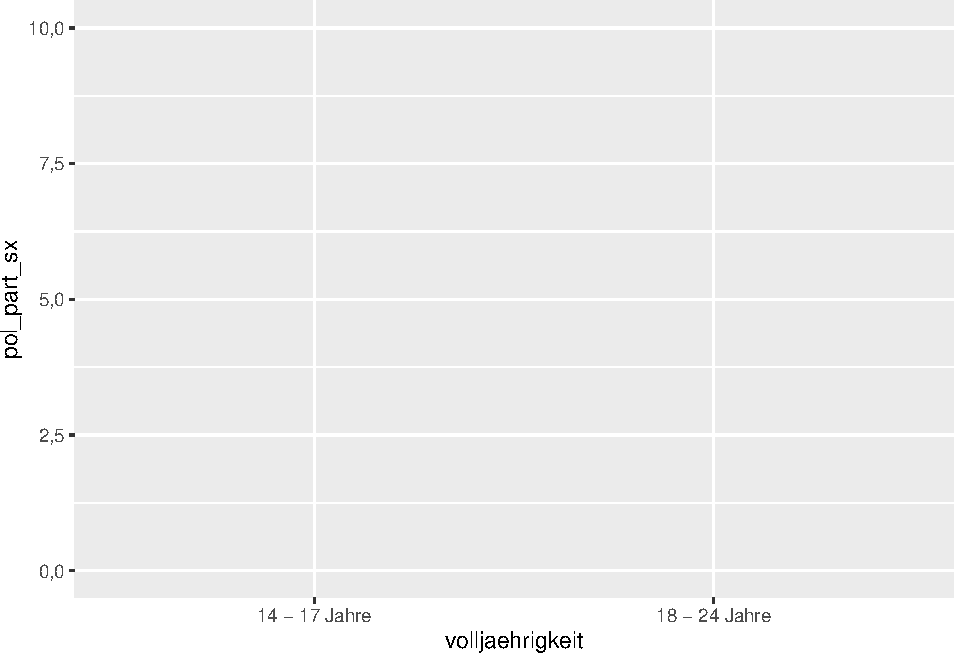
\includegraphics{r_book_files/figure-latex/unnamed-chunk-65-1.pdf}

Wie auch? Wir haben ja noch gar nicht festgelegt, um was für eine Art Grafik es sich handeln soll! Über den Operator \texttt{+} können wir dem Plot Geome hinzufügen. Wir addieren sozusagen geome zum Plot dazu: \texttt{p\ +\ geom\_()}.

\hypertarget{streudiagramm-1}{%
\subsection{Streudiagramm}\label{streudiagramm-1}}

Im ersten Schritt erstellen wir ein Streudiagramm mit \texttt{geom\_point()}.

Jedes Geom hat noch weitere (optionale) Argumente, die man entweder im aesthetic mapping verwenden kann um Variablen zuzuweisen oder man kann das allgemeine Layout dadurch verändern. Wir könnten beim Streudigramm z.B. zusätzlich zur Farbe auch die Größe der Punkte über \texttt{size} verändern oder ihre Form über \texttt{shape}.

Im Beispiel nutzen wir das zusätzliche Argument \texttt{size\ =\ 5}

\begin{Shaded}
\begin{Highlighting}[]
\CommentTok{\# Streudiagramm}
\NormalTok{p }\SpecialCharTok{+} \FunctionTok{geom\_point}\NormalTok{(}\AttributeTok{size =} \DecValTok{5}\NormalTok{)}
\end{Highlighting}
\end{Shaded}

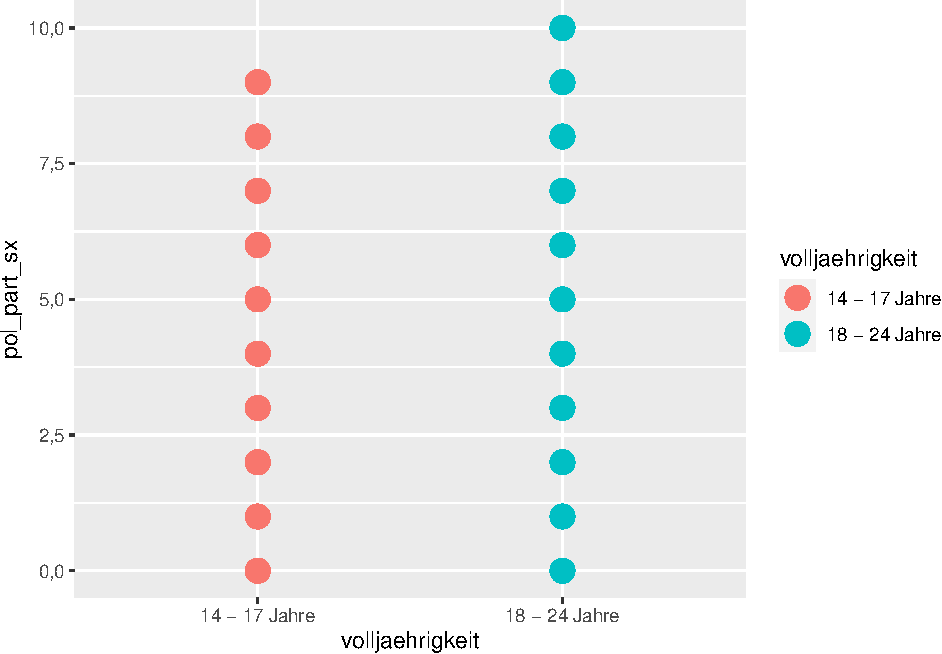
\includegraphics{r_book_files/figure-latex/unnamed-chunk-66-1.pdf}

Juhu, es hat funktioniert! Die Datenpunkte sind auf der Y-Achse angeordnet und in zwei Gruppen aufgeteilt. Die Darstellung ist jedoch suboptimal, denn die Punkte überlagern sich, sie werden vielfach übereinander geplottet. Dadurch kann man nicht wirklich gut sehen, wie sie sich verteilen.

\hypertarget{jitter-plot}{%
\subsection{Jitter-Plot}\label{jitter-plot}}

Abhilfe schafft ein alternatives Geom, nämlich \texttt{geom\_jitter()}. Beim Jitter-Plot wird jedem Punkt eine random Abweichung von den Achsen zugewiesen, so dass die Punkte zufällig streuen. Sie überlagern sich dadurch nicht mehr:

\begin{Shaded}
\begin{Highlighting}[]
\CommentTok{\# Jitter{-}Plot}
\NormalTok{p }\SpecialCharTok{+} \FunctionTok{geom\_jitter}\NormalTok{(}\AttributeTok{size =} \DecValTok{5}\NormalTok{)}
\end{Highlighting}
\end{Shaded}

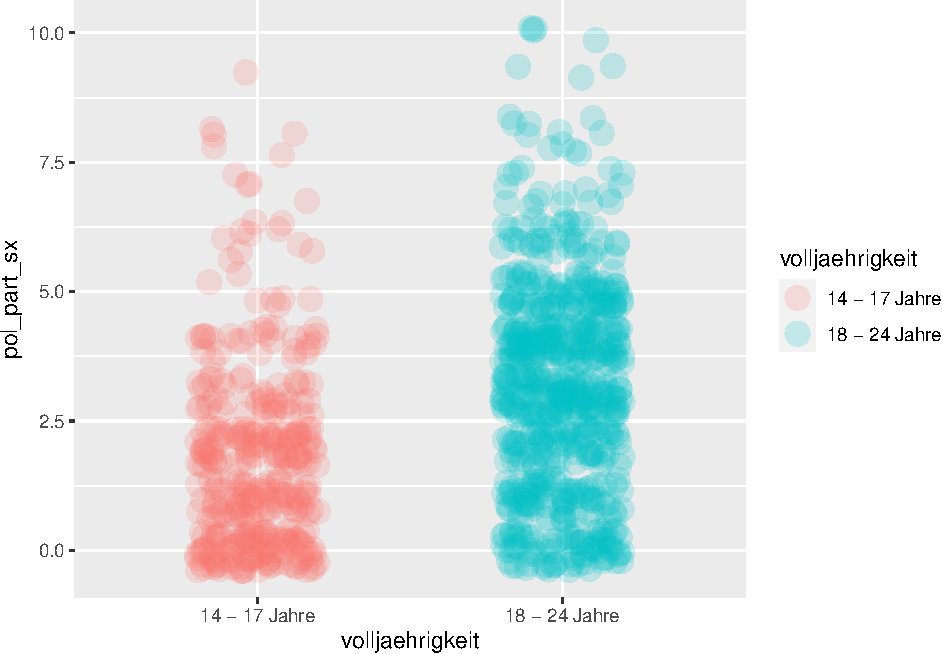
\includegraphics{r_book_files/figure-latex/unnamed-chunk-67-1.pdf}

Mit dem Argument \texttt{width} kann man die Breite dieser Streuung bestimmen und mit \texttt{alpha} die Transparenz der Punkte. Probieren wir es aus:

\begin{Shaded}
\begin{Highlighting}[]
\CommentTok{\# Jitter{-}Plot}
\NormalTok{p }\SpecialCharTok{+} \FunctionTok{geom\_jitter}\NormalTok{(}\AttributeTok{size =} \DecValTok{5}\NormalTok{, }\AttributeTok{width =} \FloatTok{0.2}\NormalTok{, }\AttributeTok{alpha =} \FloatTok{0.2}\NormalTok{)}
\end{Highlighting}
\end{Shaded}

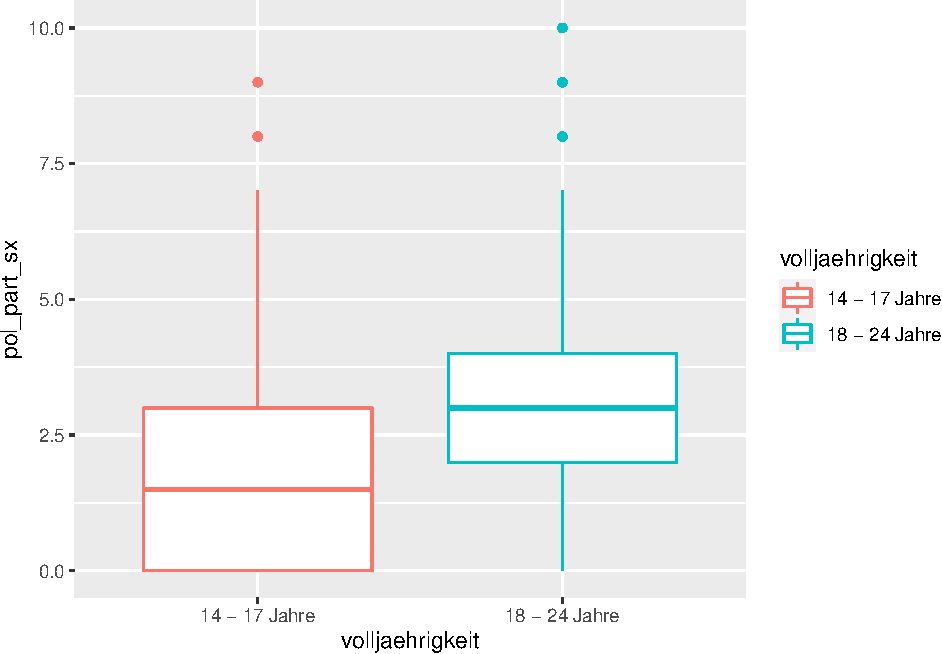
\includegraphics{r_book_files/figure-latex/unnamed-chunk-68-1.pdf}

Die Darstellung ist ganz schön, aber es gibt weitere Alternativen.

\hypertarget{boxplot}{%
\subsection{Boxplot}\label{boxplot}}

Eine weitere Möglichkeit, um die Verteilung von Variablen darzustellen, ist der Boxplot. Ein Boxplot gibt gleichzeitig Auskunft über Minimum, Maximum, die Quartilgrenzen und den Median der Verteilung einer Variable. Das mittlere Rechteck repräsentiert die mittleren 50 Prozent der Verteilung. Die „whiskers`` zeigen den 1,5-fachen Interquartilabstand. Ausreißer werden durch Punkte außerhalb der whiskers dargestellt.

Hier eine schematische Darstellung:

Und hier unser Boxplot:

\begin{Shaded}
\begin{Highlighting}[]
\CommentTok{\# Boxplot}
\NormalTok{p }\SpecialCharTok{+} \FunctionTok{geom\_boxplot}\NormalTok{()}
\end{Highlighting}
\end{Shaded}

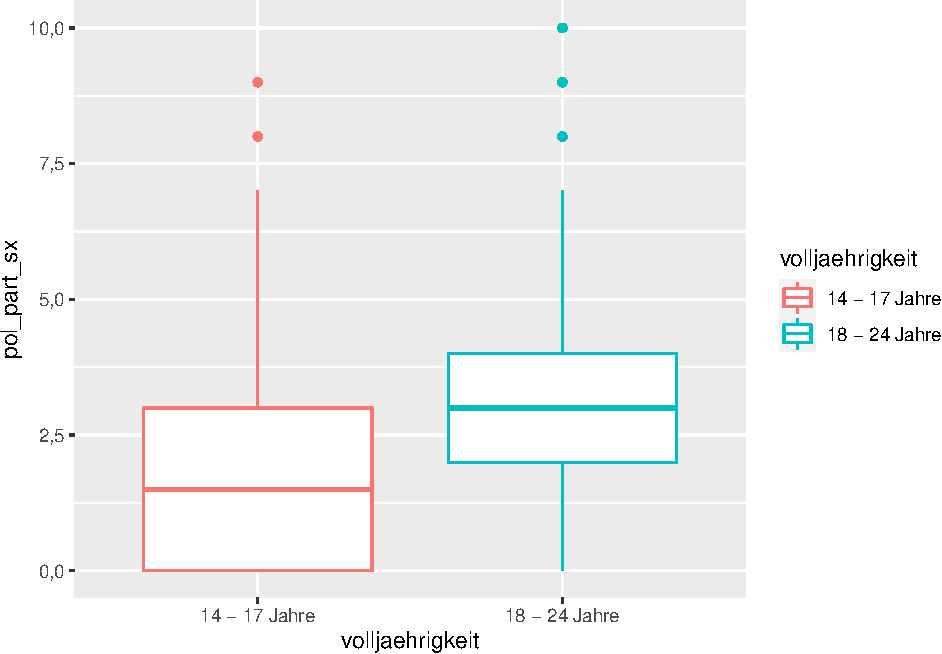
\includegraphics{r_book_files/figure-latex/unnamed-chunk-69-1.pdf}

\hypertarget{violin-plot}{%
\subsection{Violin-Plot}\label{violin-plot}}

Eine weitere Variante, um eine Verteilung darzustellen, ist der Violin-Plot. Er ähnelt dem Boxplot, er zeigt aber nicht die Quartilgrenzen, sondern die „Kerndichteschätzung``. Wenn man sich den Plot anguckt, sieht man sofort, wie unterschiedlich die Variable in den Gruppen verteilt ist:

\begin{Shaded}
\begin{Highlighting}[]
\CommentTok{\# Violon{-}Plot}
\NormalTok{p }\SpecialCharTok{+} \FunctionTok{geom\_violin}\NormalTok{()}
\end{Highlighting}
\end{Shaded}

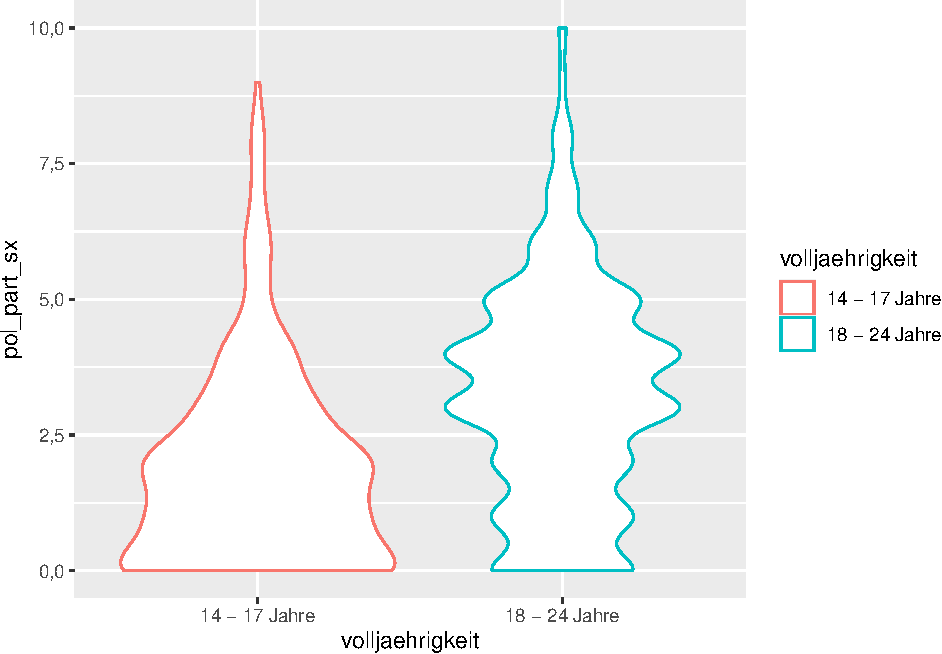
\includegraphics{r_book_files/figure-latex/unnamed-chunk-70-1.pdf}

\hypertarget{balkendiagramme}{%
\subsection{Balkendiagramme}\label{balkendiagramme}}

Für das Balkendiagramm wechseln wir jetzt mal die Variable. Balkendiagramme eignen sich ja sehr gut zur Darstellung selbst nominaler Variablen, aber ich nehme hier trotzdem mal die Lebenszufriedenheit, gemessen auf einer vierstufigen Skala.

\begin{Shaded}
\begin{Highlighting}[]
\CommentTok{\# Vorbereitung des Plots und des Mappings}
\NormalTok{p }\OtherTok{\textless{}{-}}\NormalTok{ df }\SpecialCharTok{\%\textgreater{}\%} 
  \FunctionTok{ggplot}\NormalTok{(}\AttributeTok{mapping =} \FunctionTok{aes}\NormalTok{(}\AttributeTok{x =}\NormalTok{ zufriedenheit\_leben))}
\end{Highlighting}
\end{Shaded}

Und jetzt das Geom für das Balkendiagramm hinzufügen. Weil dunkelgraue Balken so hässlich sind, färben wir sie über ´fill´ in pink ein.

\begin{Shaded}
\begin{Highlighting}[]
\CommentTok{\# Einfaches Balkendiagramm}
\NormalTok{p }\SpecialCharTok{+} \FunctionTok{geom\_bar}\NormalTok{(}\AttributeTok{fill =} \StringTok{"deeppink"}\NormalTok{)}
\end{Highlighting}
\end{Shaded}

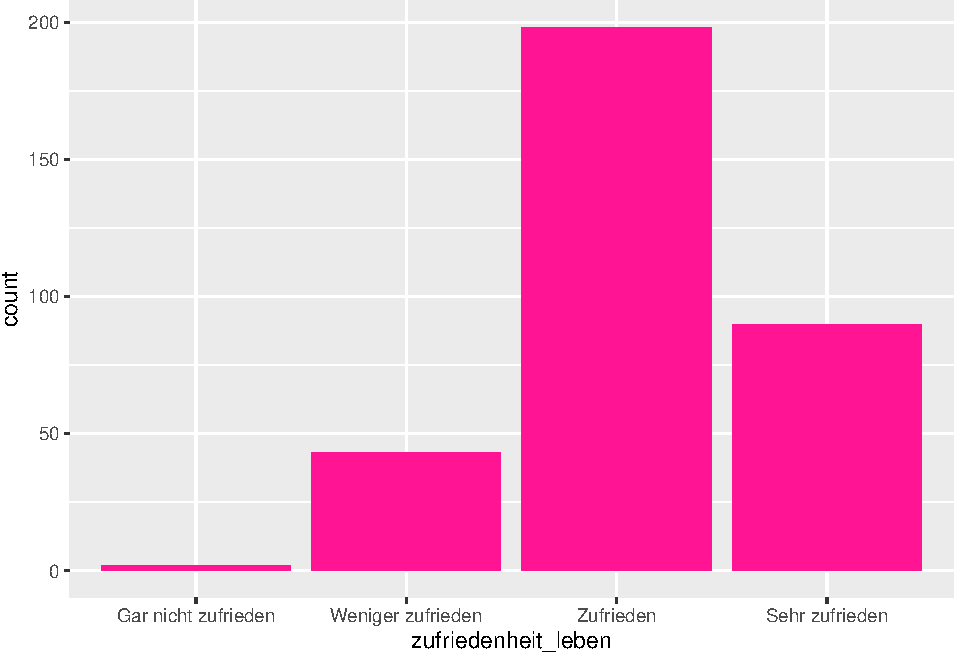
\includegraphics{r_book_files/figure-latex/unnamed-chunk-73-1.pdf}

Das Ganze kann man natürlich auch drehen, und zwar indem man dem Plot ein zusätzliches Layer mitgibt, dass das Koordinatensystem modifiziert :

\begin{Shaded}
\begin{Highlighting}[]
\CommentTok{\# horizontale Balken}
\NormalTok{p }\SpecialCharTok{+} \FunctionTok{geom\_bar}\NormalTok{(}\AttributeTok{fill =} \StringTok{"deeppink"}\NormalTok{)}\SpecialCharTok{+} 
  \FunctionTok{coord\_flip}\NormalTok{()}
\end{Highlighting}
\end{Shaded}

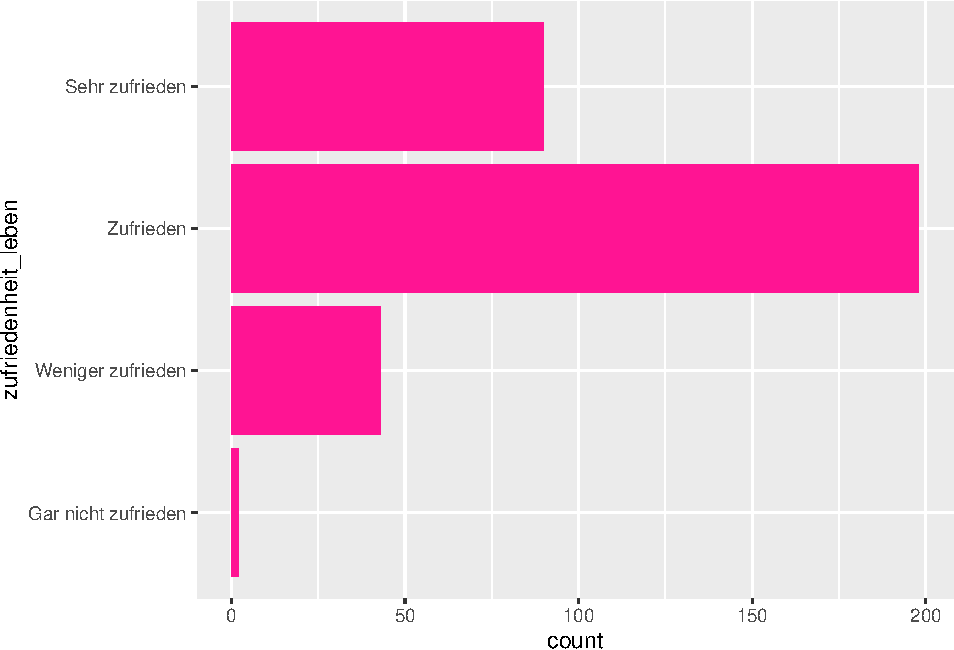
\includegraphics{r_book_files/figure-latex/unnamed-chunk-74-1.pdf}

Wenn man über \texttt{fill} eine zweite Variable mappt, bekommt man gestapelte Balken:

\begin{Shaded}
\begin{Highlighting}[]
\CommentTok{\# gestapelte Balken}
\NormalTok{p }\SpecialCharTok{+} \FunctionTok{geom\_bar}\NormalTok{(}\AttributeTok{mapping =} \FunctionTok{aes}\NormalTok{(}\AttributeTok{fill =}\NormalTok{ volljaehrigkeit)) }
\end{Highlighting}
\end{Shaded}

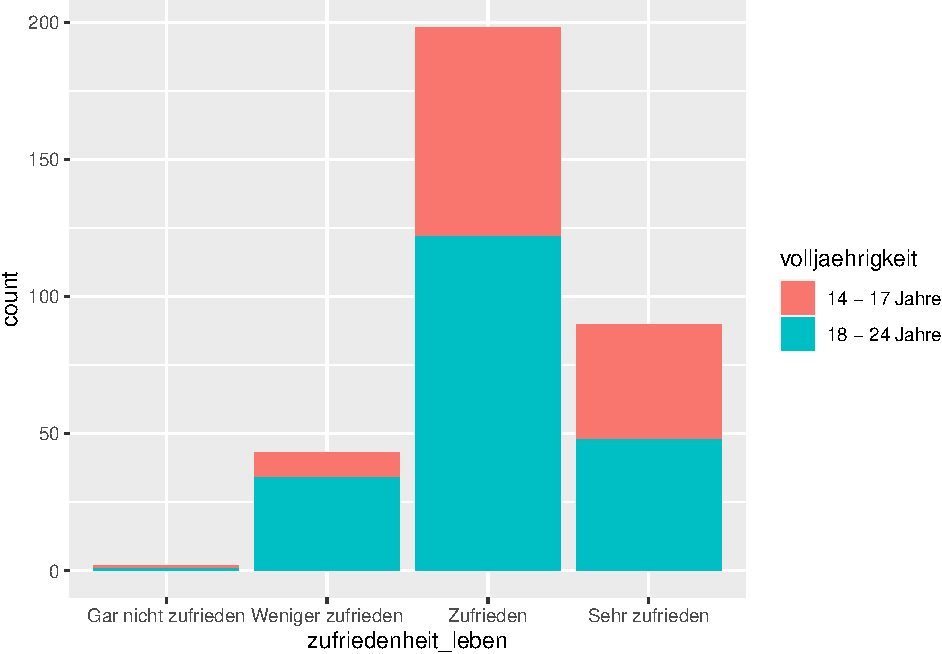
\includegraphics{r_book_files/figure-latex/unnamed-chunk-75-1.pdf}

Und über das Zusatzargument \texttt{position\ =\ "dodge"} kann man die Balken nebeneinander anzeigen. Achtung, dieses Argument wird hier außerhalb von \texttt{aes()} platziert. Es bezieht sich nämlich nicht auf das Variablen-Mapping.

\begin{Shaded}
\begin{Highlighting}[]
\CommentTok{\# Balken nebeneinander}
\NormalTok{p }\SpecialCharTok{+} \FunctionTok{geom\_bar}\NormalTok{(}\AttributeTok{mapping =} \FunctionTok{aes}\NormalTok{(}\AttributeTok{fill =}\NormalTok{ volljaehrigkeit), }\AttributeTok{position =} \StringTok{"dodge"}\NormalTok{) }
\end{Highlighting}
\end{Shaded}

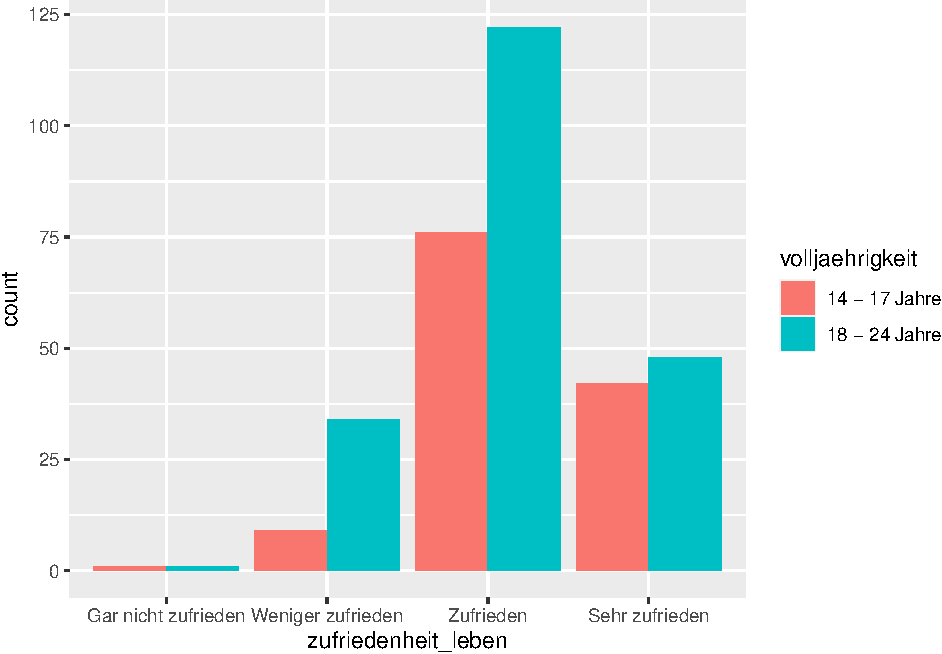
\includegraphics{r_book_files/figure-latex/unnamed-chunk-76-1.pdf}

\hypertarget{histogramme}{%
\subsection{Histogramme}\label{histogramme}}

Balkendiagramme sind prima, aber sie sind nicht für die Darstellung der Verteilung einer metrischen Variablen mit sehr vielen Ausprägungen geeignet. Nehmen wir mal als Beispiel die Mediennutzung in Minuten. Würde man für jede mögliche Ausprägung z.B. für 400 Minuten, für 401 Minuten, 402 Minuten etc. einen einzelnen Balken anfertigen, ware das sehr unübersichtlich. Es wäre schöner, würde man die Balken z.B. in Viertelstunden zusammenfassen. Ein Histogramm macht genau das.

Wir betrachten hier die Verteilung der Variable „politische Entfremdung`` (ein Mittelwertindex):

\begin{Shaded}
\begin{Highlighting}[]
\CommentTok{\# um Fehlermeldung zu vermeiden}
\NormalTok{df }\OtherTok{\textless{}{-}}\NormalTok{ df }\SpecialCharTok{\%\textgreater{}\%} 
  \FunctionTok{filter}\NormalTok{(}\SpecialCharTok{!}\FunctionTok{is.na}\NormalTok{(pol\_entfremdung\_ix))}
\end{Highlighting}
\end{Shaded}

\begin{Shaded}
\begin{Highlighting}[]
\CommentTok{\# Plot vorbereiten}
\NormalTok{p }\OtherTok{\textless{}{-}}\NormalTok{ df }\SpecialCharTok{\%\textgreater{}\%} 
  \FunctionTok{ggplot}\NormalTok{(}\AttributeTok{mapping =} \FunctionTok{aes}\NormalTok{(}\AttributeTok{x =}\NormalTok{ pol\_entfremdung\_ix))}
\end{Highlighting}
\end{Shaded}

Und jetzt das Geom hinzufügen:

\begin{Shaded}
\begin{Highlighting}[]
\CommentTok{\# Histogramm}
\NormalTok{p }\SpecialCharTok{+} \FunctionTok{geom\_histogram}\NormalTok{(}\AttributeTok{fill =} \StringTok{"deeppink"}\NormalTok{) }
\end{Highlighting}
\end{Shaded}

\begin{verbatim}
## `stat_bin()` using `bins = 30`. Pick better value with `binwidth`.
\end{verbatim}

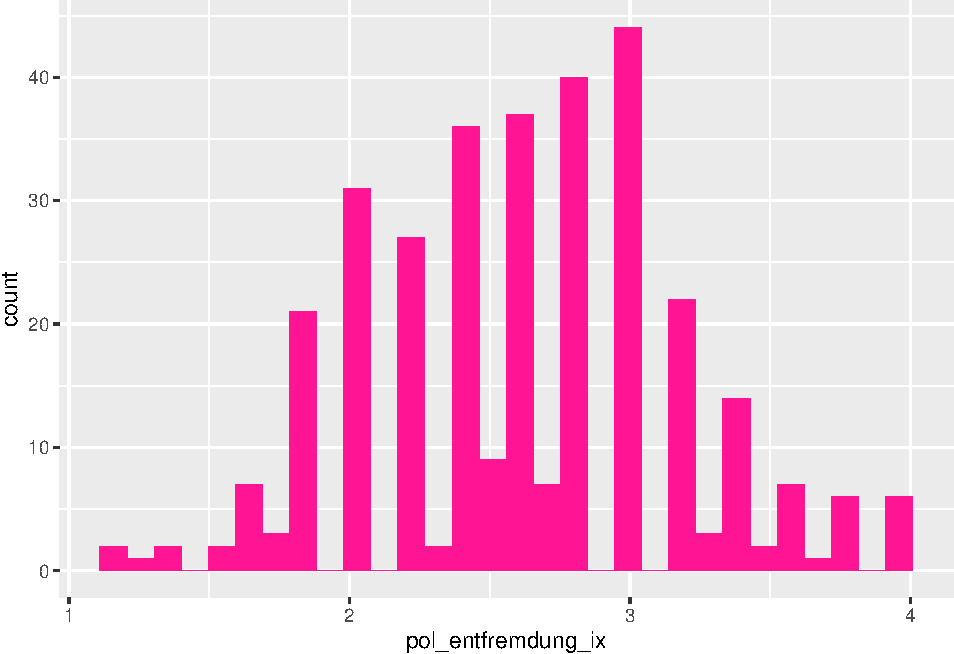
\includegraphics{r_book_files/figure-latex/unnamed-chunk-79-1.pdf}

Ohje, sehr ``löchrig''. Das ist genau das Problem, dass ich oben beschrieben hatte. Es gibt jedoch Hilfe: Mit dem Zusatzargument \texttt{binwidth} kann man zudem festlegen, in welchen Einheiten die Werte zusammengefasst werden sollen. Es lohnt sich in der Regel, ein wenig mit dieser Einstellung herumzuexperimentieren.

\begin{Shaded}
\begin{Highlighting}[]
\CommentTok{\# Histogramm mit angepasster Balkenbreite}
\NormalTok{p }\SpecialCharTok{+} \FunctionTok{geom\_histogram}\NormalTok{(}\AttributeTok{fill =} \StringTok{"deeppink"}\NormalTok{, }\AttributeTok{binwidth =} \FloatTok{0.3}\NormalTok{) }
\end{Highlighting}
\end{Shaded}

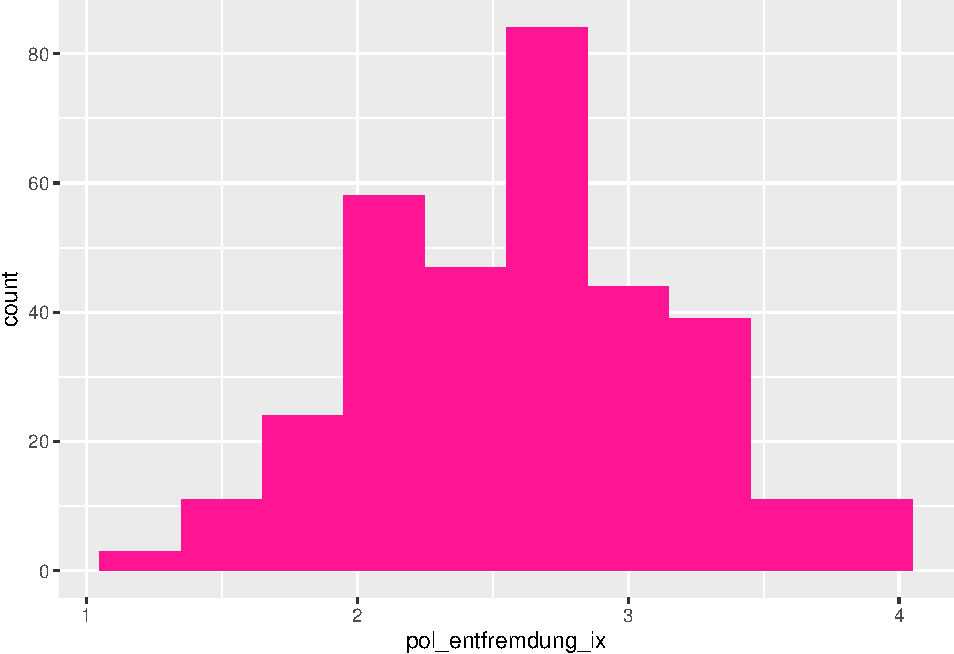
\includegraphics{r_book_files/figure-latex/unnamed-chunk-80-1.pdf}

Sieht doch gleich viel besser aus!

\hypertarget{liniendiagramme}{%
\subsection{Liniendiagramme}\label{liniendiagramme}}

Zum Abschluss folgt noch ein Liniendiagramm. Im Beispiel möchte ich die Nutzung unterschiedlicher Informationsquellen nach Alter darstellen. Das ist zwar keine richtige zeitliche Entwicklung, aber der Datensatz enthält ja nunmal auch keine Zeitreihen.

Ich möchte in dem Plot die Mittelwerte für die unterschiedlichen Informationsquellen je nach Alter darstellen. Zunächst muss der Datensatz so umgeformt werden, dass er diese Mittelwerte enthält. Ich brauche also einen kleinen Mini-Datensatz, den ich mit dplyr erzeuge.
Beginnen wir mit der Nutzung von TV-Nachrichten.

\begin{Shaded}
\begin{Highlighting}[]
\CommentTok{\# Mittelwerte Datensatz erstellen}
\NormalTok{df\_mean }\OtherTok{\textless{}{-}}\NormalTok{ df }\SpecialCharTok{\%\textgreater{}\%} 
  \FunctionTok{select}\NormalTok{(alter, }\FunctionTok{starts\_with}\NormalTok{(}\StringTok{"infoquelle\_"}\NormalTok{)) }\SpecialCharTok{\%\textgreater{}\%} 
  \FunctionTok{group\_by}\NormalTok{(alter) }\SpecialCharTok{\%\textgreater{}\%} 
  \FunctionTok{summarise}\NormalTok{(}\AttributeTok{tv\_news =} \FunctionTok{mean}\NormalTok{(infoquelle\_tv\_nachrichten, }\AttributeTok{na.rm =} \ConstantTok{TRUE}\NormalTok{),}
            \AttributeTok{google =} \FunctionTok{mean}\NormalTok{(infoquelle\_google, }\AttributeTok{na.rm =} \ConstantTok{TRUE}\NormalTok{),}
            \AttributeTok{youtube =} \FunctionTok{mean}\NormalTok{(infoquelle\_internet\_nachrichten, }\AttributeTok{na.rm =} \ConstantTok{TRUE}\NormalTok{),}
            \AttributeTok{print =} \FunctionTok{mean}\NormalTok{(infoquelle\_print, }\AttributeTok{na.rm =} \ConstantTok{TRUE}\NormalTok{),}
            \AttributeTok{tv\_satire =} \FunctionTok{mean}\NormalTok{(infoquelle\_tv\_satiere, }\AttributeTok{na.rm =} \ConstantTok{TRUE}\NormalTok{)) }
\end{Highlighting}
\end{Shaded}

Und so sieht der neue Datensatz jetzt aus:

\begin{Shaded}
\begin{Highlighting}[]
\CommentTok{\# erste Zeilen ausgeben}
\FunctionTok{head}\NormalTok{(df\_mean)}
\end{Highlighting}
\end{Shaded}

\begin{verbatim}
## # A tibble: 6 x 6
##   alter tv_news google youtube  print tv_satire
##   <dbl>   <dbl>  <dbl>   <dbl>  <dbl>     <dbl>
## 1    14   0.641  0.333   0.103 0.231     0.0513
## 2    15   0.56   0.32    0.12  0.16      0.08  
## 3    16   0.286  0.314   0.429 0.286     0.114 
## 4    17   0.55   0.15    0.35  0.2       0.2   
## 5    18   0.462  0.385   0.308 0.385     0.231 
## 6    19   0.417  0.417   0.542 0.0833    0.292
\end{verbatim}

Für das Linendiagramm benötigen wir allerdings ein \emph{Longformat}. Das bedeutet, dass die Mittelwerte der Variablen nicht neben, sondern übereinender in dem Datensatz angezeigt werden müssen. Also alle Mittelwerte werden in einer Spalte kopiert (aus fünf wird also eine Spalte). Allerdings brauchen wir dann noch eine zusätzliche Spalte/Variable, die angibt, aus welcher ursprünglichen Variable ein Mittelwert kommt.

Diese Datenumformung erreichen wir über die \texttt{dplyr}-Funktion \texttt{pivot\_longer()}. Sie benöotigt als Argument \texttt{cols}, einen Vektor, mit den die Variablen die zusammengefasst werden sollen.

\begin{Shaded}
\begin{Highlighting}[]
\CommentTok{\# von wide in long konvertieren:}
\NormalTok{df\_mean }\OtherTok{\textless{}{-}}\NormalTok{ df\_mean }\SpecialCharTok{\%\textgreater{}\%} 
  \FunctionTok{pivot\_longer}\NormalTok{(}\AttributeTok{cols =} \FunctionTok{c}\NormalTok{(tv\_news, google, youtube, print, tv\_satire))}

\CommentTok{\# erste Zeilen ausgeben}
\FunctionTok{head}\NormalTok{(df\_mean)}
\end{Highlighting}
\end{Shaded}

\begin{verbatim}
## # A tibble: 6 x 3
##   alter name       value
##   <dbl> <chr>      <dbl>
## 1    14 tv_news   0.641 
## 2    14 google    0.333 
## 3    14 youtube   0.103 
## 4    14 print     0.231 
## 5    14 tv_satire 0.0513
## 6    15 tv_news   0.56
\end{verbatim}

Genau so habe ich mir das vorgestellt. Die neuen Variablen heißen standardmäßig \texttt{name} und \texttt{value} und die Variable \texttt{alter} ist auch noch mit dabei. Genau diese Struktur und die drei Variablen brauchen wir. Jetzt kann es losgehen mit dem Liniendiagramm:

\begin{Shaded}
\begin{Highlighting}[]
\CommentTok{\# Liniendiagramm}
\NormalTok{df\_mean }\SpecialCharTok{\%\textgreater{}\%} 
  \FunctionTok{ggplot}\NormalTok{(}\AttributeTok{mapping =} \FunctionTok{aes}\NormalTok{(}\AttributeTok{x =}\NormalTok{ alter, }\AttributeTok{y =}\NormalTok{ value, }\AttributeTok{color =}\NormalTok{ name)) }\SpecialCharTok{+} 
  \FunctionTok{geom\_line}\NormalTok{()}
\end{Highlighting}
\end{Shaded}

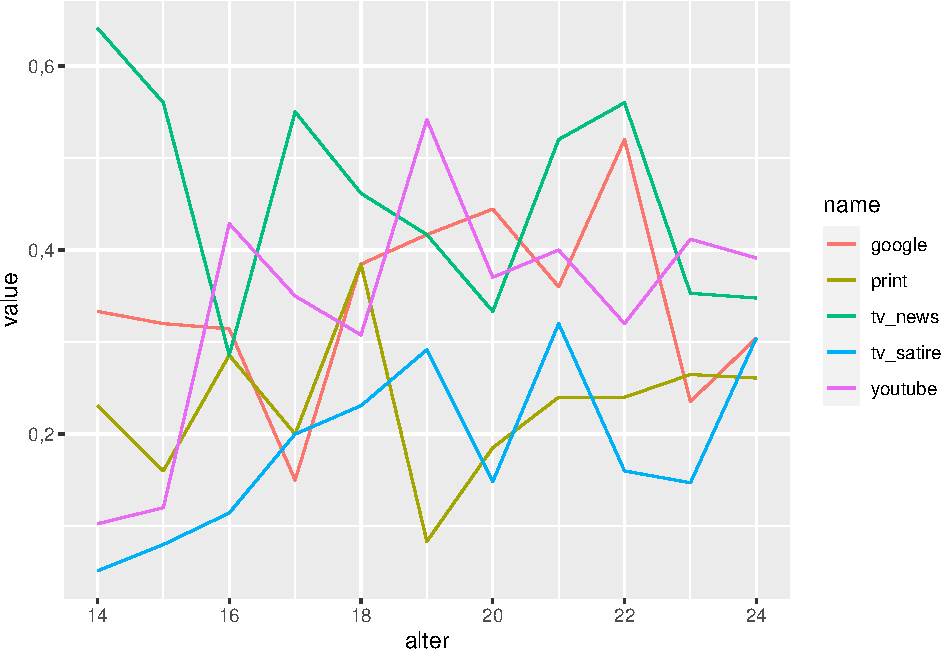
\includegraphics{r_book_files/figure-latex/unnamed-chunk-84-1.pdf}

\hypertarget{grafiken-speichern}{%
\section{Grafiken speichern}\label{grafiken-speichern}}

Natürlich können Sie die Grafiken über den ``Plot''-Tab in RStudio exportieren, um Sie in andere Programme einzufügen. Zum Abschluss möchte ich Ihnen noch eine Funktion zeigen, mit der Sie das auch direkt im Skript machen können. Die Funktion heißt \texttt{ggsave()}. Als Argumente nimmt sie beispielsweise den Dateipfad, den Namen des Plots und weitere Angaben, wie die gewünschte Höhe und Breite oder die DPI-Zahl. Außerdem kann mit \texttt{units} die Einheit für die Abmessungen festgelegt werden (z.B. \texttt{units\ =\ cm}).

\begin{Shaded}
\begin{Highlighting}[]
\CommentTok{\# den letzten angezeigten Plot speichern}
\FunctionTok{ggsave}\NormalTok{(}\AttributeTok{filename =} \StringTok{"images/my\_plot.png"}\NormalTok{)}

\CommentTok{\# einen bestimmten Plot speichern}
\FunctionTok{ggsave}\NormalTok{(}\AttributeTok{filename =} \StringTok{"images/my\_plot\_2.png"}\NormalTok{,}
       \AttributeTok{plot =}\NormalTok{ p)}
\end{Highlighting}
\end{Shaded}

\hypertarget{regression}{%
\chapter{Regression}\label{regression}}

Die Regression ist so etwas wie das ``Schweizer Taschenmesser'' der empirischen Sozialwissenschaft. Es gibt viele Varianten und Erweiterungen der Regression, der Standardfall ist jedoch die lineare Regression bzw. das lineare Modell, das ich in diesem Kapitel erläutere.

\hypertarget{das-lineare-modell}{%
\section{Das lineare Modell}\label{das-lineare-modell}}

Das lineare Modell hat die folgende Form, wobei \emph{y} für die Werte der abhängigen Variable steht (auch \emph{Outcome}, Kriterium, Regressant oder ``zu erklärende'' Variable). Die unabhängige(n) Variable(n) heißen \emph{x} (auch Prädiktoren, Regressoren oder erklärende Variablen) und \emph{b} ist ein ``Gewicht''. \emph{e} steht für den \emph{Fehler}, also den Anteil an Varianz, der nicht durch das Modell erklärt werden kann.

\[y = b_{0}+b_{1}x_{1}+b_{2}x_{2}+... b_{n}x_{n}+E\]

Das Modell besagt, dass die Ausprägung der Variable \emph{y} von den Ausprägungen der \emph{x}-Variablen abhängt. Diese \emph{x}-Variablen werden aber mit einem jeweils unterschiedlichen Gewicht \emph{b} multipliziert. Der ``Rest'', also alles, was nicht erklärt werden kann, wird mit \emph{E} aufgefangen. Das Gewicht \emph{b\_\{0\}} ist keiner \emph{x}-Variable zugeordnet. Es ist eine Art grundsätzliches Niveau von \emph{y} und wird auch als Konstante oder Achsenabschnitt (englisch Intercept) bezeichnet. - Warum zeige ich später noch.

Das \textbf{Ziel der linearen Regression} ist es herauszufinden, welche unterschiedlichen Gewichte (also Werte von \emph{b}) die einzelnen unabhängigen Variablen \emph{x} jeweils haben. Dadurch kann man eine Aussage treffen, welche Prädiktoren \emph{x} die Outcome-Variable \emph{y} in besonderem Maße beeinflussen.

-- Moment, stand da gerade \emph{beeinflussen}? Ja. Tatsächlich ist die theoretische Annahme der Regression, dass es einen Einfluss von der \emph{x}-Variable auf die \emph{y}-Variable gibt. Mit der Regression werden also Kausalhypothesen untersucht. Darin unterscheidet sie sich von der {[}\#Korrelation{]}, die lediglich von einem Zusammenhang ausgeht, ohne in abhängige und unabhängige Variable zu unterschieden.

An dieser Stelle möchte ich aber ausdrücklich darauf hinweisen, dass weder das lineare Modell noch R die Annahme der Kausalität überprüfen kann. R kann Ihnen auch nicht sagen, welche Variable in einem Modell die abhängige und welche die unabhängige sein sollte. Es ist Ihre Aufgabe als Forschende:r, sachlogische Gründe für die Plausibilität ihrer Kausalhypothese anzuführen!

\hypertarget{bivariate-lineare-regression}{%
\section{Bivariate lineare Regression}\label{bivariate-lineare-regression}}

Nach den einführenden Worten ist es jetzt Zeit für ein konkretes Beispiel. Im Folgenden möchte ich mir den einfachsten Fall vornehmen, nämlich eine Regression mit nur einem Prädiktor oder auch eine \emph{bivariate} Regression. Die Hypothese die getestet werden soll lautet:

\textbf{H1: Die politische Partizipation wird vom generellen politischen Interesse beeinflusst}

Wir nehmen uns also wieder den Gen-Z-Datensatz vor und die Variablen, um die es hier geht, kennen Sie auch schon aus den vorigen Kapiteln:

\begin{itemize}
\item
  Die abhängige Variable Politische Partizipation (\emph{y}) ist ein Summenindex von 10 politischen Handlungen, beispielsweise ``Wählen gehen'', ``Teilnahme an Produktboykott'' usw. Befragte können hier einen Wert zwischen 0 = \emph{keine Teilnahme} und 10 = \emph{Teilnahme an allen zehn Handlungen} erreichen.
\item
  Die Prädiktorvariable politisches Interesse (\emph{x}) wurde auf einer Skala von 0 = \emph{überhaupt nicht} bis 3 = \emph{sehr stark} gemessen.
\end{itemize}

Die Formel für eine bivariate Regression lautet so:

\[y = b_{0}+b_{1}x_{1}+E\]

Für unsere konkrete Hypothese bedeutet das:

\[politische Partizipation = b_{0}+b_{politisches Interesse} × politisches Interesse+Fehler\]

Sie kennen wahrscheinlich auch schon die grafische Darstellung aus den Sitzungsfolien oder aus Lehrbüchern:

\includegraphics{images/regression_model.png}

\begin{itemize}
\item
  \textbf{\emph{b\textsubscript{1}}} ist die Steigung der Regressionsgeraden (englisch \emph{slope}). Wenn wir eine Einheit auf der x-Achse weitergehen, um wie viele Einheiten steigt die Regressionsgerade dann auf der y-Achse an? Im dargestellten Beispiel sind das bei der pinken Linie zwei y-Einheiten. Bei den zur Veranschaulichung dargestellten alternativen Slopes ist die Steigung eine andere: Bei hellgrün sind es 4 (sehr steile Linie), bei hellblau nur 0,25 (sehr flach).
\item
  \textbf{\emph{b\textsubscript{0}}} ist der Achsenabschnitt, also der Punkt, an dem die Gerade die y-Achse schneidet. Anders ausgedrückt: Wenn die unabhängige Variable den Wert x = 0 hat, welchen Wert hat dann y?
\item
  Das \textbf{\emph{Residuum}} ist die Abweichung der Messpunkte von der Regressionsgerade. Hier dargestellt durch einen einzelnen blauen Punkt (die Messung), der eben nicht genau auf der pinken Linie liegt. Der Fehler \textbf{\emph{E}} in der Regressionsgleichung wird in der Regel \textbf{gebildet durch die Summe der quadrierten Residuen}. Das hat dann den Vorteil, dass positive und negative Residuen sich nicht gegenseitig aufheben können und dass größere Abweichungen proportional stärker ins Gewicht fallen als kleinere. Es ist aber vor allem eine Konvention. Denkbar wäre es auch, den Fehler durch die Summe der Beträge der Residuen zu bilden. Macht aber keiner.
\end{itemize}

\leavevmode\hypertarget{info_e}{}%
\textbf{Warum gibt es überhaupt Residuen und den Fehler?}

Der Fehler basiert auf allen Abweichungen der gemessenen Werte vom Modell der Regressionsgeraden (Residuen). Empirisch wird sich nämlich kaum eine perfekte Anordnung zeigen, bei der alle Messpunkte genau auf der Geraden liegen. In einer Messung wird es immer Punkte geben, die mehr oder weniger stark von der Regressionsgerade abweichen. In unserem Beispiel könnte es eine Person geben, die sich erst an 4 politischen Handlungsmöglichkeiten beteiligt hat, die aber dennoch angibt, ihr politisches Interesse sei extrem hoch. Für diese Abweichung kann es natürlich ganz unterschiedliche Gründe geben. Die empirische Wirklichkeit ist eben kein Modell! Hier ein paar unterschiedliche Beispiele, wie die Abweichung zustande kommen kann:

\begin{itemize}
\item
  Die Person hat die Skala für politisches Interesse falsch herum gedeutet, sie wollte eigentlich ein niedriges politisches Interesse angeben. - Also ein ``Fehler'' beim Ausfüllen des Fragebogens.
\item
  Die Person hatte einfach noch nicht genügend Gelegenheit, sich an politischen Aktionen zu beteiligen. Vielleicht ist sie sehr jung und hat deshalb nicht die Möglichkeit zu Demonstrationen in die nächste Stadt zu fahren oder zu wählen. Es könnte also sein, dass unser Modell unvollständig ist und noch nicht alle relevanten Einflussfaktoren berücksichtigt sind.
\item
  Der Wert, den unsere Regressionsgerade vorhersagt, ist empirisch gar nicht erreichbar. Es könnte zum Beispiel sein, dass die modellhafte Gerade vorhersagt, dass eine Person, deren politisches Interesse bei ``3'' liegt, ``5,2'' politische Handlungen ausgeführt haben müsste. - Das geht ja kaum. Der Wert, den die Gerade schätzt, ist eben nur hypothetisch.
\item
  Der Zusammenhang ist gar nicht linear (also keine gerade Linie). Vielleicht wäre eine ``andere Form'' der Line viel angemessener. Vielleicht eine Kurve die erst steil ansteigt und dann abflacht.
\end{itemize}

In jeder tatsächlich durchgeführten Berechnung einer Regression liegt wahrscheinlich eine Mischung aus verschiedenen Gründen vor. Was genau sich hinter dem Residuum genau verbirgt, werden wir nie wirklich wissen. Es ist jedoch natürlich unsere Aufgabe, den Wert mit einem gut durchdachten Forschungsdesign möglichst klein zu halten.

Bevor es jetzt losgeht, noch eine kleine Anmerkung zu der Kausalannahme der Hypothese: Allgemein wird häufig davon ausgegangen, dass das Denken das Handeln prägt. Deshalb ist die Hypothese grundsätzlich plausibel. Häufig ist jedoch durchaus auch eine umgekehrte Richtung plausibel. Auch in diesem Fall könnte es durchaus sein, dass die Teilnahme an politischen Aktionen wie Demonstrationen oder Wahlen Einfluss auf das politische Interesse ausübt. Nehmen wir mal an, wir haben einen langen Theorieteil geschrieben und die Unterteilung in unabhängige und abhängige Variable hinreichend begründet.

\hypertarget{grafische-darstellung}{%
\subsection{Grafische Darstellung}\label{grafische-darstellung}}

Die erste Annäherung an die Regression ist grafisch. Mit einem Scatterplot oder Jitterplot kann der Zusammenhang zwischen zwei Variablen visualisiert werden (vgl. Abschnitt {[}\#\#\# Streudiagramm{]}). Das Paket \texttt{ggplot2} kann aber noch mehr. Mit dem Geom \texttt{geom\_smooth} kann man über \texttt{method\ =\ "lm"} (für ``linear model'') eine Regressionsgerade zur Punktewolke hinzufügen.

\begin{Shaded}
\begin{Highlighting}[]
\NormalTok{data }\SpecialCharTok{\%\textgreater{}\%} 
  \FunctionTok{ggplot}\NormalTok{(}\FunctionTok{aes}\NormalTok{(}\AttributeTok{x =}\NormalTok{ politisches\_interesse, }\AttributeTok{y =}\NormalTok{ pol\_part\_sx)) }\SpecialCharTok{+}
  \FunctionTok{geom\_jitter}\NormalTok{() }\SpecialCharTok{+}
  \FunctionTok{geom\_smooth}\NormalTok{(}\AttributeTok{method =} \StringTok{"lm"}\NormalTok{, }\AttributeTok{se =} \ConstantTok{FALSE}\NormalTok{, }\AttributeTok{color =} \StringTok{"deeppink"}\NormalTok{) }\SpecialCharTok{+}
  \FunctionTok{xlab}\NormalTok{(}\StringTok{"politisches Interesse"}\NormalTok{) }\SpecialCharTok{+}
  \FunctionTok{ylab}\NormalTok{(}\StringTok{"politische Partizipation"}\NormalTok{)}
\end{Highlighting}
\end{Shaded}

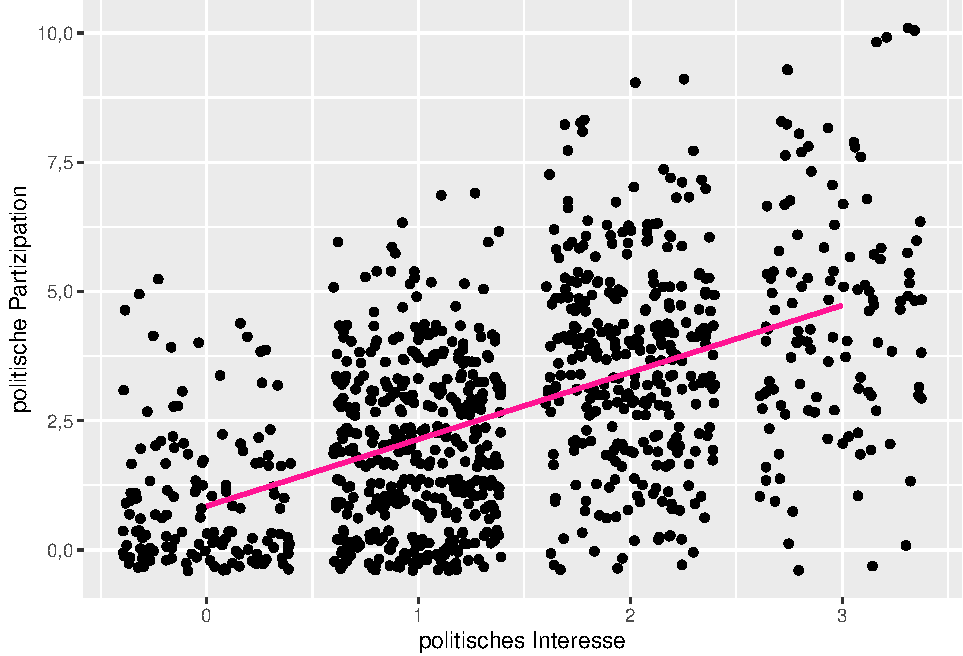
\includegraphics{r_book_files/figure-latex/unnamed-chunk-87-1.pdf}

Prima, das sieht ja schon super aus! Und definitiv nach einem positiven Zusammenhang. - Aber welche Werte haben jetzt \emph{b\textsubscript{0}} und vor allem \emph{b\textsubscript{1}}? Dazu mehr im nächsten Abschnitt.

Zunächst möchte ich noch kurz auf das \texttt{geom\_smooth()} eingehen. Oben habe ich der Funktion drei Argumente mitgegeben. Das erste Argument, \texttt{method}, hatte ich auf \texttt{lm} gesetzt, weil wir ja hier genau das machen wollen -- nämlich eine Regressionsgerade nach dem ``linearen Modell'' berechnen. Denkbar wären natürlich auch andere Modelle (z.B. Kurven). Beim letzten Argument \texttt{color\ =\ "deeppink"} können Sie sich wahrscheinlich schon denken was es macht: Es färbt die Gerade in CI-konformen HMTMH-Magenta ein. Aber was macht das mittlere Argument \texttt{se\ =\ FALSE}? Das finden wir ganz einfach heraus, indem wir es einmal auf \texttt{TRUE} setzen:

\begin{Shaded}
\begin{Highlighting}[]
\NormalTok{data }\SpecialCharTok{\%\textgreater{}\%} 
  \FunctionTok{ggplot}\NormalTok{(}\FunctionTok{aes}\NormalTok{(}\AttributeTok{x =}\NormalTok{ politisches\_interesse, }\AttributeTok{y =}\NormalTok{ pol\_part\_sx)) }\SpecialCharTok{+}
  \FunctionTok{geom\_jitter}\NormalTok{() }\SpecialCharTok{+}
  \FunctionTok{geom\_smooth}\NormalTok{(}\AttributeTok{method =} \StringTok{"lm"}\NormalTok{, }\AttributeTok{se =} \ConstantTok{TRUE}\NormalTok{, }\AttributeTok{color =} \StringTok{"deeppink"}\NormalTok{) }\SpecialCharTok{+}
  \FunctionTok{xlab}\NormalTok{(}\StringTok{"politisches Interesse"}\NormalTok{) }\SpecialCharTok{+}
  \FunctionTok{ylab}\NormalTok{(}\StringTok{"politische Partizipation"}\NormalTok{)}
\end{Highlighting}
\end{Shaded}

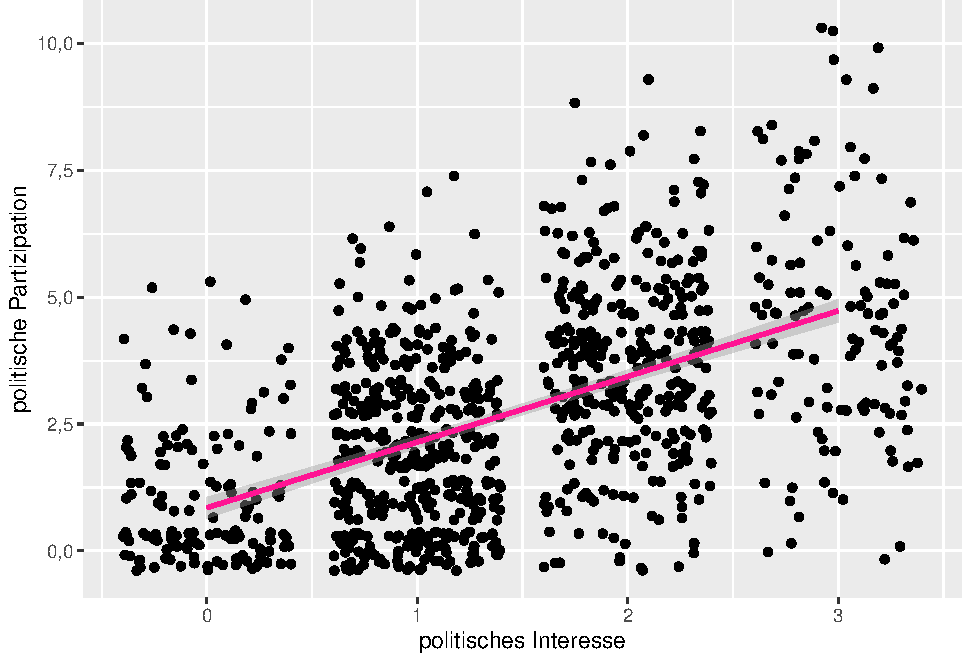
\includegraphics{r_book_files/figure-latex/unnamed-chunk-88-1.pdf}

Hmm. Viel hat sich nicht verändert. Aber jetzt ist da so ein ``Schatten'' hinter der Geraden. Dieser Schatten zeigt das Konfidenzintervall der Regressionsgeraden an. Praktisch!

\hypertarget{die-funktion-lm}{%
\subsection{\texorpdfstring{Die Funktion \texttt{lm()}}{Die Funktion lm()}}\label{die-funktion-lm}}

Die grafische Darstellung ist sehr nützlich, aber natürlich wüssten wir auch gerne die genauen Werte für unsere Regressionsgerade. Um die herauszufinden, bietet das \texttt{stats}-Paket die Funktion \texttt{lm()} (linear model). Zur Erinnerung: Genau wie \texttt{base}-R muss man das \texttt{stats}-Paket nicht gesondert laden, es ist standardmäßig verfügbar, sobald man RStudio öffnet.

Die Funktion \texttt{lm()} erwartet zwei Argumente: 1. ein Objekt der R-Klasse ``formula''. Das ist eine neue Art von Objekt, die bisher noch nicht vorkam. Mit so einer ``Formel'' teilt man R mit, mit welchen Variablen ein Modell gerechnet werden soll und wie die Variablen miteinander zusammenhängen. Für letzteres gibt es verschiedene Operatoren. 2. als zweites Argument benötigt die Funktion natürlich noch den Datensatz, auf den die Formel angewendet werden soll.

Für die bivariate Regression müssen wir nun zuerst eine Formel formulieren, also unsere Hypothese für R so übersetzen, dass es sie versteht und die Regression berechnen kann. Dazu benötigen wir den Operator \texttt{\textasciitilde{}} (Tilde). \textbf{Die Tilde \texttt{\textasciitilde{}} bedeutet: ``wird vorhergesagt durch''}. Für die lineare Regression muss die Formel also \texttt{abhängige\_Variable\ \ \textasciitilde{}\ unabhängige\_Variable} lauten.

Nachdem man die \texttt{lm()}-Funktion ausgeführt und das Ergebnis einem selbst benannten Objekt (z.B. \texttt{my\_model}) zugeordnet hat, kann man sich mit der \texttt{summary()}-Funktion die Ergebnisse der Regression anzeigen lassen. In unserem Beispiel sieht das ganze so aus:

\begin{Shaded}
\begin{Highlighting}[]
\CommentTok{\# Model formulieren}
\NormalTok{my\_model }\OtherTok{\textless{}{-}} \FunctionTok{lm}\NormalTok{(pol\_part\_sx }\SpecialCharTok{\textasciitilde{}}\NormalTok{ politisches\_interesse, }\AttributeTok{data =}\NormalTok{ data)}
  
\CommentTok{\# Zusammenfassung ausgeben}
\FunctionTok{summary}\NormalTok{(my\_model)}
\end{Highlighting}
\end{Shaded}

\begin{verbatim}
## 
## Call:
## lm(formula = pol_part_sx ~ politisches_interesse, data = data)
## 
## Residuals:
##     Min      1Q  Median      3Q     Max 
## -4,7303 -1,1427 -0,1427  1,0042  5,5635 
## 
## Coefficients:
##                       Estimate Std. Error t value Pr(>|t|)    
## (Intercept)            0,84886    0,10594   8,013 3,12e-15 ***
## politisches_interesse  1,29382    0,06332  20,431  < 2e-16 ***
## ---
## Signif. codes:  0 '***' 0,001 '**' 0,01 '*' 0,05 '.' 0,1 ' ' 1
## 
## Residual standard error: 1,746 on 997 degrees of freedom
##   (7 Beobachtungen als fehlend gelöscht)
## Multiple R-squared:  0,2951, Adjusted R-squared:  0,2944 
## F-statistic: 417,4 on 1 and 997 DF,  p-value: < 2,2e-16
\end{verbatim}

Puh, da steht eine Menge Zeug. Vieles davon habe ich noch gar nicht erklärt. Gehen wir den Output der Reihe nach durch.

Der Output beginnt mit dem \textbf{Call}. Das ist ganz nett, hier wird unser Funktionsaufruf wiederholt. Er ist also im Model mit abgespeichert: Ein kleiner Reminder, falls man viele Modelle gerechnet und vergessen hat, welche Formel und Daten man jeweils benutzt hat.

Dann folgen die \textbf{Residuals}. Die Residuen sind die Abweichungen der Messwerte von den Werten, die die Regressionsgerade für jeden Fall im Datensatz vorhersagen würde. Also der Fehler oder das, was oben in der einleitenden Grafik mit \emph{e} gekennzeichnet war. Wenn man sich den Scatterplot von oben anschaut, dann ist das Residuum die Distanz von jedem einzelnen Punkt zur Regressionsgeraden. Liegt der Punkt über der Regressionsgerade, hat das Residuum ein positives Vorzeichen. Liegt ein Punkt darunter, ist das Vorzeichen negativ.

Im Output der \texttt{lm()}-Funktion werden hier einfach ein paar zentrale Kennzahlen über die Verteilung der Residuen angegeben, nämlich die Quartilsgrenzen. Wir könnten uns aber auch für jeden Fall im Datensatz das jeweilige Residuum ausgeben lassen. Schön wäre natürlich, wenn die Residuen möglichst klein wären. Das ist hier aber leider nicht der Fall. Die Werte weichen bis zu \text{-4,73} nach unten und sogar bis zu \text{5,56} nach oben ab.

Die Werte für \emph{b\textsubscript{0}} und \emph{b\textsubscript{1}} finden sich im dritten Bereich der Ausgabe unter \textbf{Coefficients} in der Spalte ``Estimate'':

\begin{itemize}
\tightlist
\item
  In der Zeile ``(Intercept)'' ist der Wert für \emph{b\textsubscript{0}} (hier \text{0,85})
\item
  In der Zeile ``politisches\_interesse'' ist der Wert für \emph{b\textsubscript{1}} (hier \text{1,29})
\end{itemize}

Die weiteren Spalten in der Coefficients-Tabelle enthalten den Standardfehler (``Std. Error'') für die b-Werte und jeweils noch einen t-Test (vgl. zukünftiges Kapitel ``t-Test''). Der t-Test prüft, ob die b-Werte überzufällig von Null abweichen. Seine Test-Statistik ist der t-Wert (``t value'') und zu diesem t-Wert gibt es noch ein Signifikanzniveau (``Pr(\textgreater\textbar t\textbar)''). Wie immer gilt hier, dass ein Wert von p \textless{} .05 als signifikant gewertet wird. Praktischerweise sind signifikante Werte in der Tabelle mit Sternchen \texttt{*} gekennzeichnet. Was die Sternchen und die anderen Codes genau bedeuten, ist praktischerweise unter der Tabelle nochmal aufgeführt.

\leavevmode\hypertarget{info_b}{}%
\textbf{Was sagen die Regressionskoeffizienten (b-Werte) aus?}

Der Wert \emph{b\textsubscript{1}} = \text{1,29} gibt an, um wie viele Einheiten die abhängige Variable ansteigt oder abfällt, wenn der Prädiktor um eine Einheit größer wird. Hier also: Nimmt das politische Interesse um 1 zu (also z.B. von 2 = \emph{Weniger stark} auf 3 = \emph{Eher stark}) dann kommen \text{1,29} politische Handlungen dazu.

Der Wert \emph{b\textsubscript{0}} = \text{1,3} bedeutet, dass die abhängige Variable ``politische Partizipation'' den Wert \text{1,3} annimmt, wenn die unabhängige Variable = 0 ist. Tatsächlich, in unserer Grafik oben schneidet die Regressionsgerade die y-Achse genau bei diesem Wert. Aus dem positiven Intercept kann man schließen, dass es offenbar ein gewisses Grundniveau von politischer Partizipation gibt. -- Selbst wenn kein politisches Interesse vorliegt (0 = \emph{Überhaupt nicht}), gibt es laut der Regressionsgerade eine gewisse politische Partizipation.

Im vierten und letzten Abschnitt des Outputs wird der Standardfehler der Residuen inklusive Freiheitsgerade (degrees of freedom) angegeben (Erläuterung folgt später). An dieser Stelle erfährt man auch, dass einige Fälle aus der Berechnung entfernt wurden, da sie fehlende Werte in der einen oder anderen Variable aufweisen.

Zu guter Letzt gibt es noch einen R\textsuperscript{2}-Wert (r-squared), ein korrigiertes R\textsuperscript{2} (adjustet R-squared) und eine F-Statistik für eben dieses R\textsuperscript{2}. R\textsuperscript{2} ist der Anteil, der durch den Prädiktor erklärten Varianz an der Gesamtvarianz der abhängigen Variable. Mit dem F-Test im Output wird hier wiederum geschaut, ob R\textsuperscript{2} sich signifikant von Null unterschiedet. -- So ähnlich wie oben mit dem t-Test bei den b-Werten.

Wenn man eine Regression berechnet, gibt man diese in der Regel in Form einer Tabelle an. Eine einzelne Regression kann aber auch textlich berichtet werden. Neben \emph{b\textsubscript{1}} (inkl. Signifikanzniveau) sollte außerdem unbedingt mindestens R\textsuperscript{2} inklusive der Freiheitsgrade und dem Signifikanzniveau angegeben werden. Der Intercept wird in Tabellen mit berichtet, auch wenn er kaum interpretiert wird.

\begin{Shaded}
\begin{Highlighting}[]
\NormalTok{sign }\OtherTok{\textless{}{-}} \FunctionTok{case\_when}\NormalTok{(}
   \FunctionTok{glance}\NormalTok{(my\_model)}\SpecialCharTok{$}\NormalTok{p.value[[}\DecValTok{1}\NormalTok{]]}\SpecialCharTok{\textless{}}\FloatTok{0.001} \SpecialCharTok{\textasciitilde{}} \StringTok{"p \textless{} .001"}\NormalTok{,}
   \FunctionTok{glance}\NormalTok{(my\_model)}\SpecialCharTok{$}\NormalTok{p.value[[}\DecValTok{1}\NormalTok{]]}\SpecialCharTok{\textless{}}\FloatTok{0.01} \SpecialCharTok{\textasciitilde{}} \StringTok{"p \textless{} .01"}\NormalTok{,}
   \FunctionTok{glance}\NormalTok{(my\_model)}\SpecialCharTok{$}\NormalTok{p.value[[}\DecValTok{1}\NormalTok{]]}\SpecialCharTok{\textless{}}\FloatTok{0.05} \SpecialCharTok{\textasciitilde{}} \StringTok{"p \textless{} .05"}\NormalTok{,}
   \ConstantTok{TRUE} \SpecialCharTok{\textasciitilde{}} \StringTok{"n.s."}
\NormalTok{)}
\end{Highlighting}
\end{Shaded}

Das Ergebnis für unsere Hypothese von oben lautet wie folgt: Die Daten bestätigen die Hypothese. Die politische Partizipation wird vom generellen politischen Interesse beeinflusst. Steigt das politische Interesse um einen Skalenpunkt, so geht dies mit einer Zunahme von \emph{b} = \text{1,29} politischen Handlungen einher. Die erklärte Varianz beträgt R\textsuperscript{2} = \text{0,2951303}, bei df = \text{997} Freiheitsgraden (korrigiertes R\textsuperscript{2} = \text{0,2944233}). Das Modell ist auf dem Niveau p \textless{} .001 signifikant.

\hypertarget{standardisierte-regressionskoeffizienten-ux3b2}{%
\subsection{Standardisierte Regressionskoeffizienten (β)}\label{standardisierte-regressionskoeffizienten-ux3b2}}

Neben den normalen Regressionskoeffizienten b kann man auch den standardisierten Koeffizienten β (beta) berechnen. Dazu \textbf{z-standardisiert} man die Messwerte zuerst oder formt die Regressionsgleichung entsprechend um. Durch die Standardisierung wird die Skalierung der einzelnen Messwerte herausgerechnet, Z-Standardisierung bedeutet ja ``auf den Mittelwert zentrieren und Standardabweichung = 1 setzen''. Eine standardisierte Prädiktorvariable ist nicht mehr im oben genannten Sinn interpretierbar, denn wenn der Wert der standardisierten Variable sich um 1 erhöht, dann ist das eben keine Einheit mehr (also \textbf{nicht} der Sprung von 2 = \emph{Weniger stark} auf 3 = \emph{Eher stark}) sondern eine Erhöhung um eine Standardabweichung (was immer das heißt). Die standardisierten β-Werte haben aber einen anderen Vorteil: Sollte man mehrere Prädiktoren in einem Modell haben, die aber auf unterschiedlichen Skalen gemessen wurden (z.B. 1x 5er und 1x 7er Skala), kann man ihren relativen Erklärungsbeitrag besser untereinander vergleichen.

Das \texttt{stats}-Paket kann die β-Koeffizienten nicht direkt berechnen. Dazu gibt es aber das Paket \texttt{lm.beta} mit der gleichnamigen Funktion, welche auf ein mit \texttt{lm()} erzeugtes Modell angewendet werden kann.

\begin{Shaded}
\begin{Highlighting}[]
\CommentTok{\# Paket laden}
\FunctionTok{library}\NormalTok{(lm.beta)  }

\CommentTok{\# beat{-}Koeffizienten ausgeben}
\FunctionTok{lm.beta}\NormalTok{(my\_model) }
\end{Highlighting}
\end{Shaded}

\begin{verbatim}
## 
## Call:
## lm(formula = pol_part_sx ~ politisches_interesse, data = data)
## 
## Standardized Coefficients::
##           (Intercept) politisches_interesse 
##              0,000000              0,543259
\end{verbatim}

\leavevmode\hypertarget{info_beta}{}%
\textbf{Achtung b oder β?}

Leider gibt es bezüglich \emph{b} und \emph{β} -- wie so oft -- ein wenig Begriffs-Chaos in unterschiedlichen Lehrbüchern. Manchmal wird nämlich für die hier mit \emph{b} betitelten nicht-standardisierten Regressionskoeffizienten \emph{β} genutzt.

\hypertarget{t-tests}{%
\chapter{T-Tests}\label{t-tests}}

\emph{Die Erarbeitung dieses Kapitels erfolgte auf Basis eines Skripts, welches Daniel Possler 2021 für die Veranstaltung SDA2 erstellt hat. Gegenüber dem Skript aus der Veranstaltung wurde jedoch das Datenbeispiel erweitert, damit der Einstichproben-T-Test demonstriert werden kann. Außerdem wurden die Funktionen auf ein tidyverse-konformes Paket (\texttt{rstatix}) angepasst.}

In diesem Kapitel werden verschiedene Varianten des T-Tests behandelt. Bei T-Test geht es immer um den Vergleich von Mittelwerten, also um Unterschiedshypothesen.
Als T-Tests werden eine Reihe von Null-Hypothesen-Tests bezeichnet, deren Prüfgröße auf der T-Verteilung basiert.
T-Tests wurden ursprünglich von William S. Gosset entwickelt, der für die Guinness-Brauerei daran arbeitete, die Qualität der Gerste abzuschätzen, damit das Bier einen gleichbleibenden Qualitätsstandard erfüllen konnte.
Gosset entwickelte den T-Test und wollte seine Erkenntnisse gerne mit anderen Forschenden teilen.
Da Guinness die Offenbarung von Betriebsgeheimnissen fürchtete, war es Mitarbeitenden der Brauerei jedoch verboten, ihre Erkenntnisse unter ihrem Namen zu veröffentlichen.
Gosset nutzte deshalb das Pseudonym ``Student''.
T-Tests sind deshalb heute auch als ``Student´s T-Test'' bekannt.

Es gibt verschiedene Varianten des T-Tests, von den hier drei besprochen werden:

\begin{itemize}
\item
  Beim diesem \textbf{Ein-Stichproben-T-Test} (1-sample-test) wird geprüft, ob sich ein das arithmetische Mittel (Mittelwert) von einem zuvor festgelegten Wert unterscheidet.
\item
  Mit dem \textbf{T-Test für unabhängige Stichproben} (2-sample-test, t-test for independent samples) kann man prüfen, ob sich die Mittelwerte einer bestimmten Variable in zwei Populationen voneinander unterscheiden. -- Verglichen wird also der Mittelwert in ein und dieselben Variable aber in zwei Gruppen.
\item
  Der \textbf{T-Test für abhängige Stichproben} (t-test for paired samples) testet, ob sich zwei miteinander zusammenhängende Mittelwerte von einander unterschieden. Die Stichproben, die verglichen werden, hängen also irgendwie miteinander zusammen. Das kann z.B. der Fall bei einer Vorher- und einer Nachher-Messung in einem Experiment sein. Oder wenn in einem Datensatz beide Partner:innen einer Beziehung befragt werden. Oder wenn einfach zwei verschiedene Kennwerte miteinander vergleichen werden sollen. Im Datensatz liegen die beiden ``Stichproben'' also als zwei verschiedene Variablen vor.
\end{itemize}

\hypertarget{datenbeispiel}{%
\section{Datenbeispiel}\label{datenbeispiel}}

In den folgenden Analysen wird ein Beispieldatensatz mit per Zufallsgenerator erzeugten Daten verwendet, den Daniel Possler und ich erstellt haben.
In der fiktiven Studie, zu der der Datensatz gehört, soll untersucht werden, ob das Spielen von unterschiedlichen Videospielen einen Einfluss auf die Spendenbereitschaft (pro-soziales Verhalten) hat.

Konkret beinhalten die Daten ein Experimentaldesign, in dem geprüft wird, ob die Spendenbereitschaft davon abhängt, ob die Proband:innen in einem Videospiel einen Superhelden steuern oder nicht.

Für eine Baseline-Messung war vor dem Gebäude, in dem die Studie stattfand, ein Schauspieler platziert, der sich als Obdachloser ausgab.
Er bat jede:n Proband:in, bevor er/sie zur Studie hereinkam, um ``eine kleine Spende''.
Der Betrag, den die Proband:innen dem Schauspieler gaben wurde in den Datensatz eingetragen (Variable: \emph{Spende\_t0}).

Im Anschluss wurden die N = 70 Versuchspersonen zufällig und gleichmäßig auf zwei Experimentalgruppen aufgeteilt (n₁ = 35 und n₂ = 35; Variable: \emph{Gruppe}).

\begin{itemize}
\item
  Gruppe 1 wurde gebeten, zwanzig Minuten lang ein Superhelden-Spiel zu spielen.
\item
  Gruppe 2 spielte hingegen genauso lange ein Rennspiel.
\end{itemize}

Zum Dank erhielten die Proband:innen eine Aufwandsentschädigung von 10 Euro. Es wurde ihnen die Möglichkeit eingeräumt, dieses Geld für einen wohltätigen Zweck zu spenden -- entweder vollständig oder teilweise.
Die Höhe der Spende wurde für jede Versuchsperson erfasst (Variable: \emph{Spende\_t1}).

Um die Stabilität der Effekte untersuchen zu können, wurden die Proband:innen drei Tage nach der Teilnahme noch einmal eingeladen.
Sie erhielten wieder eine Aufwandsentschädigung von 10 Euro und konnten erneut einen Teil oder die vollständige Summe spenden (Variable: \emph{Spende\_t2}).

Hier ein kurzer Blick in den Datensatz:

\begin{Shaded}
\begin{Highlighting}[]
\FunctionTok{head}\NormalTok{(df\_prosocial)}
\end{Highlighting}
\end{Shaded}

\begin{verbatim}
## # A tibble: 6 x 5
##     Vpn Gruppe            Spende_t0 Spende_t1 Spende_t2
##   <dbl> <chr>                 <dbl>     <dbl>     <dbl>
## 1     1 Superhelden-Spiel         3         7         3
## 2     2 Superhelden-Spiel         3         8         1
## 3     3 Superhelden-Spiel         0        10         3
## 4     4 Superhelden-Spiel         3         9         3
## 5     5 Superhelden-Spiel         3        10         2
## 6     6 Superhelden-Spiel         1         7         2
\end{verbatim}

\hypertarget{einstichproben-t-test}{%
\section{Einstichproben-T-Test}\label{einstichproben-t-test}}

Der Einstichproben-T-Test kommt häufig zum Einsatz. Z. B. immer dann, wenn in einer Regression getestet wird, ob sich die Regressionskoeffizienten signifikant von \emph{Null} unterscheiden.
Der Wert, gegen den getestet wird, ist in dem Fall einfach Null.
Es ist aber auch möglich, gegen einen anderen, selbst festgelegten Wert zu testen.

Mit dem Einstichproben-T-Test könnte man z. B. die folgenden Hypothesen auf den Prüfstand stellen:

\begin{itemize}
\item
  Der IQ in einer Gruppe von Befragten unterscheidet sich signifikant vom Wert 100.
\item
  Die politische Einstellung auf einer links-rechts-Skala weicht deutlich nach rechts vom Skalenmittel ab.
\item
  Die Länge von Zeit-Online-Artikeln liegt über 3.000-Zeichen.
\end{itemize}

Die \textbf{Anwendungsvoraussetzung} für den Einstichproben-T-Test ist das Datenniveau. Die betrachtete Variable muss logischerweise \textbf{intervallskaliert} sein -- bei nominalem oder ordinalem Datenniveau würde die Berechnung eines arithmetischen Mittels ja auch keinen Sinn ergeben.

\hypertarget{hypothese-aufstellen}{%
\subsection{Hypothese aufstellen}\label{hypothese-aufstellen}}

In unserem Fallbeispiel möchten wir zunächst untersuchen, wie es allgemein um das prosoziale Verhalten der Versuchspersonen bestellt ist -- ganz unabhängig von dem Experiment. Wir nutzen dazu die Variable \emph{Spende\_t0} und klären die Frage, ob die Versuchspersonen dem vermeintlichen Obdachlosen im Mittel mehr oder weniger als einen bestimmten Wert gespendet haben. Da es sich bei den Werten in der Variable um Angaben in Euro handelt, erfüllt die Variable das erforderliche Datenniveau.

Bevor es mit dem T-Test losgehen kann, muss noch eine Hypothese aufgestellt werden. Wir müssen einen Wert festlegen, gegen den wir testen wollen. Diesen Wert können wir frei wählen, wir könnten z.B. schauen ob die Spenden signifikant über Null liegen oder von 1,50 Euro abweichen. Normalerweise müsste die Hypothese natürlich begründet werden, aber ich lege sie jetzt einfach mal wie folgt fest:

\emph{H1: Die Spendenbereitschaft der Versuchspersonen liegt zum Zeitpunkt T0 signifikant über 1,50 Euro.}

Diese Hypothese ist einseitig gerichtet. Sie gilt als zutreffend, wenn (1) der Mittelwert der Variable \emph{Spende\_t0} größer als 1,5 ist und (2) der T-Test ein signifikantes Ergebnis zeigt.

\hypertarget{daten-explorieren}{%
\subsection{Daten explorieren}\label{daten-explorieren}}

Natürlich empfiehlt es sich immer vor einer Analyse die Verteilung seiner Variablen zu kennen und sie durch Grafiken und deskriptive Statistiken zu explorieren. Gut geeignet erscheint in diesem Fall ein einfaches Bar-Chart, bei metrischen Variablen mit sehr vielen Ausprägungen wäre ein Histogramm besser:

\begin{Shaded}
\begin{Highlighting}[]
\NormalTok{df\_prosocial }\SpecialCharTok{\%\textgreater{}\%} 
  \FunctionTok{ggplot}\NormalTok{(}\FunctionTok{aes}\NormalTok{(}\AttributeTok{x =}\NormalTok{ Spende\_t0)) }\SpecialCharTok{+}
  \FunctionTok{geom\_bar}\NormalTok{() }
\end{Highlighting}
\end{Shaded}

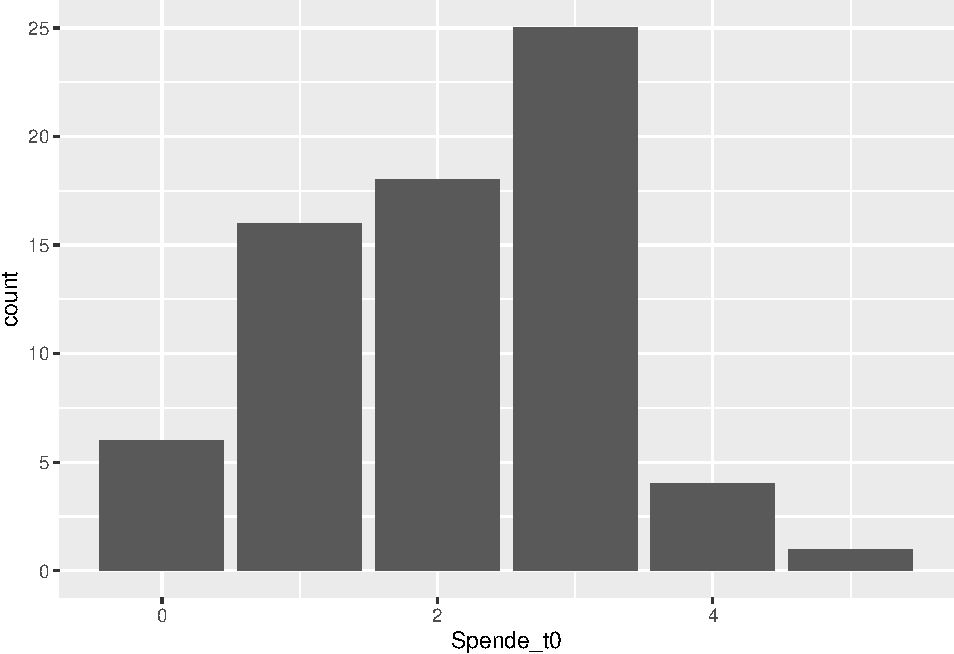
\includegraphics{r_book_files/figure-latex/unnamed-chunk-94-1.pdf}

Oh! Sehr schön, viele Versuchspersonen sind spendabel! -- Und halbwegs normalverteilt sieht der Plot sogar auch aus\ldots{} er ist ein wenig linksschief.

\leavevmode\hypertarget{info_levene}{}%
\textbf{Normalverteilung der Variablen? -- Nicht nötig!}

Manchmal wird angegeben, dass die ``Normalverteilung der Variablen in der Grundgesamtheit'' (wahlweise auch ``in der Stichprobe'') eine Anwendungsvoraussetzung für den T-Test sei. Dies ist nicht der Fall! Das Verfahren wäre dann auch ziemlich eingeschränkt, denn für Variablen, die nun einmal einfach ``schief'' verteilt sind und natürlicherweise nicht normalverteilt vorliegen (wie bspw. Alter oder Einkommen), könnte man es nicht anwenden.

Richtig ist: Der T-Test setzt lediglich voraus, dass sich Stichprobenmittelwerte über verschiedene Samples hinweg normal verteilen -- was nach zentralem Grenzwerttheorem bei randomisierten Stichproben der Fall sein sollte (\href{https://www.youtube.com/watch?v=jvoxEYmQHNM}{hier} meine Lieblings-Erklärung zum zentralen Grenzwertsatz).

Mit deskriptiven Statistiken können wir herausfinden, wo der Mittelwert der Verteilung liegt, beispielsweise könnte man dazu die \texttt{mean()}- Funktion benutzen. Die \texttt{describe()}-Funktion aus \texttt{psych} liefert noch ein umfassenderes Bild:

\begin{Shaded}
\begin{Highlighting}[]
\FunctionTok{library}\NormalTok{(psych)}

\FunctionTok{describe}\NormalTok{(df\_prosocial}\SpecialCharTok{$}\NormalTok{Spende\_t0)}
\end{Highlighting}
\end{Shaded}

\begin{verbatim}
##    vars  n mean  sd median trimmed mad min max range skew kurtosis   se
## X1    1 70  2,1 1,1      2     2,1 1,5   0   5     5 -0,1     -0,6 0,14
\end{verbatim}

Tatsächlich, der Mittelwert liegt bei \text{2,1}, also deutlich über 1,5 Euro. Das spricht schon einmal für die Hypothese H1. Aber wie sieht es mit der zweiten Bedingung aus? Dazu benötigen wir den Signifikanzwert des T-Tests.

\hypertarget{t-test-durchfuxfchren}{%
\subsection{T-Test durchführen}\label{t-test-durchfuxfchren}}

Der T-Test ist im stats-Package von R bereits mit eingebaut und zwar über die Funktion \texttt{t.test()}. Man kann aber auch das Paket \texttt{rstatix} und dessen Funktion \texttt{t\_test()} benutzen. Das Paket hat es sich zum Ziel gesetzt, für einfache statistische Tests eine tidyverse-Variante anzubieten. Deshalb kann die Funktion \texttt{t\_test()} in der Pipe verwendet werden, was später noch nützlich sein wird. Und sie liefert als Ergebnis einen tibble zurück, der in der Ausgabe sehr übersichtlich ist und der sich leicht in eine APA-konforme Darstellung umbauen lässt.

Die wichtigsten Argumente der \texttt{t\_test()}-Funktion aus \texttt{rstatix} werden hier kurz erläutert:

\begin{enumerate}
\def\labelenumi{\arabic{enumi}.}
\item
  Das Datenargument, also den Datensatz, der die Variablen enthält. Wie im Tidyverse üblich kann man ihn als erstes Argument über die Pipe übergeben.
\item
  Eine Formel, die die statistische Modellierung nach R übersetzt. Solche Formeln sind schon aus dem Kapitel \protect\hyperlink{regression}{Regression} bekannt. Die Tilde \texttt{\textasciitilde{}} verbindet dabei die Variablen der Analyse mit einander. Tilde bedeutet übersetzt in Worte an dieser Stelle etwa ``die Variable vor der Tilde wird verglichen mit dem Wert nach der Tilde''. Die Notation ist immer \texttt{Variable1\ \textasciitilde{}\ Variable2}. Im Fall des Einstichproben-T-Tests gibt es jedoch nur eine Variable und die entsprechende Formel lautet \texttt{Variable1\ \textasciitilde{}\ 1}.
\item
  Über \texttt{mu} kann der Testwert angegeben werden. Lässt man das Argument weg, wird automatisch vom Testwert ``0'' ausgegangen.
\item
  Mit \texttt{alternative} lässt sich festlegen, ob der Test ein- oder zweiseitig erfolgen soll, wobei letzteres der Standard ist. Möchte man einseitig prüfen muss man konkret angeben, ob der Mittelwert \emph{kleiner} als der Testwert sein soll (\texttt{"less"}) oder \emph{größer} (\texttt{"greater"}).
\item
  Mit \texttt{detailed=\ TRUE} kann eine ausführlichere Darstellung angefordert werden. Standardmäßig ist das Argument jedoch auf \texttt{FALSE} gesetzt.
\end{enumerate}

Fordern wir zunächst die nicht-detaillierte Standard-Ausgabe an:

\begin{Shaded}
\begin{Highlighting}[]
\FunctionTok{library}\NormalTok{(rstatix)}

\NormalTok{df\_prosocial }\SpecialCharTok{\%\textgreater{}\%} 
  \FunctionTok{t\_test}\NormalTok{(Spende\_t0 }\SpecialCharTok{\textasciitilde{}} \DecValTok{1}\NormalTok{, }\AttributeTok{mu =} \FloatTok{1.5}\NormalTok{, }\AttributeTok{alternative =} \StringTok{"greater"}\NormalTok{) }
\end{Highlighting}
\end{Shaded}

\begin{verbatim}
## # A tibble: 1 x 7
##   .y.       group1 group2         n statistic    df         p
## * <chr>     <chr>  <chr>      <int>     <dbl> <dbl>     <dbl>
## 1 Spende_t0 1      null model    70      4.52    69 0.0000123
\end{verbatim}

Die Tabelle fasst das Ergebnis zusammen. Weiter vorne in der Tabelle finden sich ein paar Angaben zum durchgeführten Test, z.B. der Name der Variable und die Fallzahl n.~Das in der Spalte ``group1'' eine 1 und unter ``group2'' nur ``null model'' steht, zeigt an, dass hier ein Einstichproben-T-Test durchgeführt wurde. Wichtig ist aber insbesondere, was hinten in der Tabelle steht: Unter ``statistic'' wird der T-Wert ausgegeben. Die Spalte ``df'' liefert die entsprechenden Freiheitsgrade und p den zum T-Wert gehörigen Signifikanzwert. Da p kleiner als .05 ist, kann die Hypothese als bestätigt angenommen werden.

Über das Argument \texttt{detailed\ =\ TRUE} erhält mannoch eine ausführlichere Darstellung die auch die Difefrenz zwischen Mittelwert und Testwert sowie die Grenzen des Konfidenzintervalls enthält. Da die Tabelle sehr breit ist, kann sie hier nicht dargestellt werden. Aber probieren Sie es gerne aus!

\hypertarget{cohens-d}{%
\subsection{Cohen´s d}\label{cohens-d}}

Das \texttt{rstatix}-Paket enthält auch eine Funktion zur Berechnung der Effektstärke in Form von Cohen´s d (\texttt{cohens\_d()}). Die Funktion benötigt als Argumente dieselbe Formel wie der zugehörige T-Test und natürlich auch den Test-Wert:

\begin{Shaded}
\begin{Highlighting}[]
\NormalTok{df\_prosocial }\SpecialCharTok{\%\textgreater{}\%} 
  \FunctionTok{cohens\_d}\NormalTok{(Spende\_t0 }\SpecialCharTok{\textasciitilde{}} \DecValTok{1}\NormalTok{, }\AttributeTok{mu =} \FloatTok{1.5}\NormalTok{) }
\end{Highlighting}
\end{Shaded}

\begin{verbatim}
## # A tibble: 1 x 6
##   .y.       group1 group2     effsize     n magnitude
## * <chr>     <chr>  <chr>        <dbl> <int> <ord>    
## 1 Spende_t0 1      null model   0.541    70 moderate
\end{verbatim}

Die Ausgabe fasst noch einmal den Test zusammen und nennt unter ``effsize'' den Wert für Cohen´s d.~In der letzten Spalte wird außerdem eingeordnet, wie stark der Effekt ist. Die Grenzen für die Einordnung der Effektstärke sind die, die Cohen selbst nennt \citep{Cohen_1992}: \textbar d\textbar{} \textless{} 0.2 ``negligible'', \textbar d\textbar{} \textless{} 0.5 ``small'', \textbar d\textbar{} \textless{} 0.8 ``moderate'', \textbar d\textbar{} \textgreater= ``large''.

Abschließend können wir die Hypothese H1 positiv beurteilen: Der Mittelwert M = \text{2,11} der Variable Spende\_t0 unterscheidet sich tatsächlich auf dem Niveau p \textless{} ,001 vom Testwert 1,5 (t(\text{69}) = \text{4,52}). Cohen´s d = \text{0,54} bescheinigt eine mittlere Effektstärke.

\leavevmode\hypertarget{info_levene}{}%
\textbf{T-Tests mit dem stats-Paket}

Für T-Tests benötigt man eigentlich gar kein Zusatzpaket, weil die Funktion \texttt{t.test()} bereits im stats-Pakage (also in base-R) eingebaut ist (man beachte den ``.'' statt des "\_"). Allerdings hat die Funktion \texttt{t.test()} den Nachteil, dass sie nicht mit der Pipe verwendbar ist und das Paket liefert auch keinen Levene-Test -- ebensowenig wie Cohen´s d.~Beides könnte man zwar auch über andere Pakete erhalten (z.B. \texttt{car} und \texttt{effsize}), aber mit \texttt{rstatix} erhält man alles aus einer Hand und tidyverse-konform.

Zur Vollständigkeit kommt hier noch die base-R-Syntax, inklusive Output:

\begin{Shaded}
\begin{Highlighting}[]
\FunctionTok{t.test}\NormalTok{(}\AttributeTok{x =}\NormalTok{ df\_prosocial}\SpecialCharTok{$}\NormalTok{Spende\_t0, }\AttributeTok{mu =} \FloatTok{1.5}\NormalTok{, }\AttributeTok{alternative =} \StringTok{"greater"}\NormalTok{)   }
\end{Highlighting}
\end{Shaded}

\begin{verbatim}
## 
##  One Sample t-test
## 
## data:  df_prosocial$Spende_t0
## t = 5, df = 69, p-value = 1e-05
## alternative hypothesis: true mean is greater than 1,5
## 95 percent confidence interval:
##  1,9 Inf
## sample estimates:
## mean of x 
##       2,1
\end{verbatim}

Die Zahlen sind die gleichen, es gibt nur Abweichungen durch Rundung (base-R rundet den T-Wert auf ganze Zahlen). Da die Vorteile des \texttt{rstatix}-Paketes überwiegen, beschreibe ich die base-Syntax hier nicht weiter. Ausführlich findet sich das z. B. bei bei \citet{Phillips_2018} in Kapitel 13.3.

Die Logik des Einstichproben-T-Tests ist ganz einfach: Wir haben erstens einen fixen, selbst festgelegten Wert (hier 1,5, aber häufig ist es 0). Zweitens gibt es einen Wert, der in gewisser Weise ``variabel'' ist, nämlich abhängig von der Stichprobe. Für diesen variablen Wert wird ein Konfidenzintervall berechnet. Liegt jetzt der feste Testwert außerhalb des Konfidenzintervalls des Stichprobenwertes, können wir annehmen, dass sich die beiden Werte tatsächlich signifikant unterscheiden. (Der p-Wert hat im Prinzip die gleiche Aussage: Er drückt aus wie (un)wahrscheinlich es ist, den errechneten Mittelwert zu erhalten, wenn in der Grundgesamtheit eigentlich der Testwert der Mittelwert wäre.)

\hypertarget{t-test-fuxfcr-unabhuxe4ngige-stichproben}{%
\section{T-Test für unabhängige Stichproben}\label{t-test-fuxfcr-unabhuxe4ngige-stichproben}}

Der T-Test für unabhängige Stichproben führt die Logik Einstichproben-T-Tests fort. Der Unterschied ist hier einfach nur, dass es nicht jeweils einen fixen Wert und einen errechneten Mittelwert gibt, sondern zwei ``variable'' Mittelwerte aus eben zwei unterschiedlichen Teilstichproben. Der T-Test für unabhängige Stichproben berechnet die Differenz zwischen den Mittelwerten und überprüft, ob diese signifikant von Null abweicht.

Um das ganze etwas konkreter zu machen, hier ein paar typische Hypothesen, die man mit dem T-Test für unabhängige Stichproben testen kann:

\begin{itemize}
\item
  Männer und Frauen unterschieden sich in ihrem politischen Interesse.
\item
  Rentner:innen sehen täglich länger fern als Studierende.
\item
  Die Artikel auf Zeit-Online sind länger als die auf Spiegel-Online.
\item
  Eine Gruppe mit Versuchspersonen die Treatment 1 (rote Pille) bekommen hat, reagiert völlig anders als eine andere Gruppe von Versuchspersonen, die Treatment 2 (grüne Pille) bekommen hat.
\end{itemize}

Wie in den Beispielen leicht zu erkennen ist, betreffen die Hypothesen jeweils zwei Variablen. Beim T-Test für unabhängige Stichproben unterscheidet man zwischen einer unabhängigen und einer abhängigen Variable. -- Mindestens implizit wird von einer Ursache-Wirkungs-Beziehung ausgegangen. Die unabhängige Variable bildet die beiden Gruppen. Sie ist zwingend nominal-dichotom, denn mehr als zwei Gruppen kann man mit einem T-Test nicht vergleichen (für mehr als zwei Gruppen würde man eine Varianzanalyse verwenden). Der Mittelwert wird für die abhängige Variable berechnet, und zwar getrennt voneinander zweimal, also für beide Gruppen.

Im Rechen-Beispiel kommen wir wieder auf das Videospiel-Experiment zum prosozialen Verhalten zurück. Die Forscher haben die folgende Hypothese aufgestellt:

\emph{H2: Bei Spieler:innen die ein Superhelden-Spiel gespielt haben, ist die Spendenbereitschaft höher als bei denen, die ein Rennspiel gespielt haben.}

\hypertarget{deskriptive-auswertung}{%
\subsection{Deskriptive Auswertung}\label{deskriptive-auswertung}}

Natürlich bietet es sich an, zunächst einmal rein deskriptiv zu prüfen, ob die Mittelwerte sich überhaupt und in der prognostizierten Richtung unterscheiden. Dazu kann man auf Mittel aus dplyr zurückgreifen:

\begin{Shaded}
\begin{Highlighting}[]
\NormalTok{df\_prosocial }\SpecialCharTok{\%\textgreater{}\%} 
  \FunctionTok{group\_by}\NormalTok{(Gruppe) }\SpecialCharTok{\%\textgreater{}\%} 
  \FunctionTok{summarise}\NormalTok{(}\AttributeTok{M =} \FunctionTok{mean}\NormalTok{(Spende\_t1, }\AttributeTok{na.rm =} \ConstantTok{TRUE}\NormalTok{), }
            \AttributeTok{SD =} \FunctionTok{sd}\NormalTok{(Spende\_t1, }\AttributeTok{na.rm =} \ConstantTok{TRUE}\NormalTok{), }
            \AttributeTok{n =} \FunctionTok{n}\NormalTok{())}
\end{Highlighting}
\end{Shaded}

\begin{verbatim}
## # A tibble: 2 x 4
##   Gruppe                M    SD     n
##   <chr>             <dbl> <dbl> <int>
## 1 Rennspiel          2.76  1.58    35
## 2 Superhelden-Spiel  7.91  1.78    35
\end{verbatim}

Das sieht schonmal vielversprechend aus! Ein illustrativer Boxplot ist eine aussagekräftige grafische Variante:

\begin{Shaded}
\begin{Highlighting}[]
\NormalTok{df\_prosocial }\SpecialCharTok{\%\textgreater{}\%} 
  \FunctionTok{filter}\NormalTok{(}\SpecialCharTok{!}\FunctionTok{is.na}\NormalTok{(Spende\_t1)) }\SpecialCharTok{\%\textgreater{}\%} 
  \FunctionTok{ggplot}\NormalTok{(}\FunctionTok{aes}\NormalTok{(Gruppe, Spende\_t1, }\AttributeTok{color =}\NormalTok{ Gruppe)) }\SpecialCharTok{+}
  \FunctionTok{geom\_boxplot}\NormalTok{() }\SpecialCharTok{+}
  \FunctionTok{theme}\NormalTok{(}\AttributeTok{legend.position =} \StringTok{"none"}\NormalTok{)}
\end{Highlighting}
\end{Shaded}

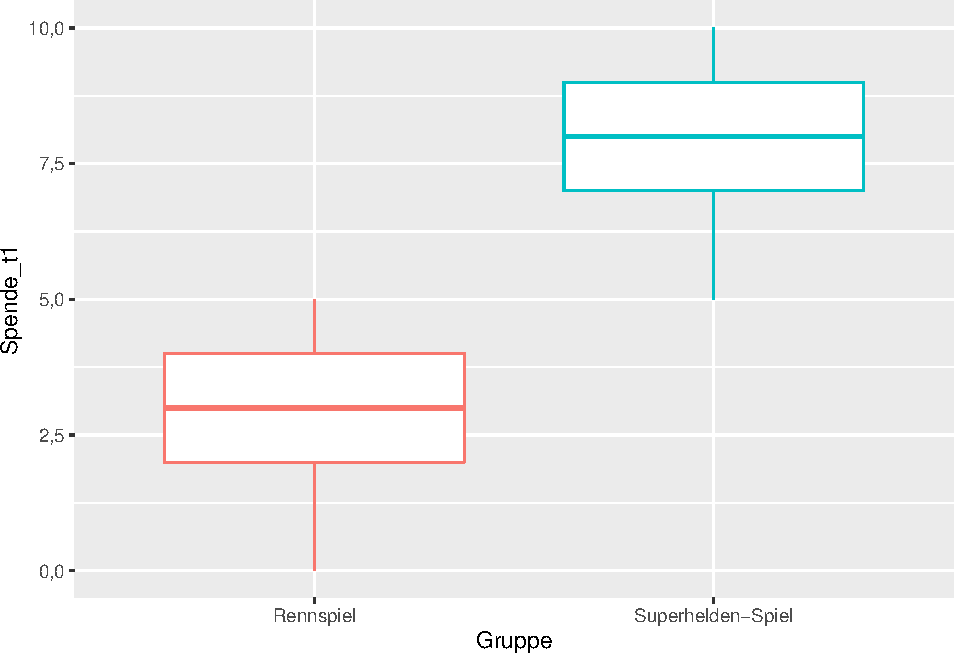
\includegraphics{r_book_files/figure-latex/unnamed-chunk-101-1.pdf}

Noch eine Variation: Mit zwei übereinanderliegenden Density-Plots (eine Art ``geglättetes Histogramm'') kann man ebenfalls die Lage und Verteilung beider Variablen gut vergleichen:

\begin{Shaded}
\begin{Highlighting}[]
\NormalTok{df\_prosocial }\SpecialCharTok{\%\textgreater{}\%} 
  \FunctionTok{filter}\NormalTok{(}\SpecialCharTok{!}\FunctionTok{is.na}\NormalTok{(Spende\_t1)) }\SpecialCharTok{\%\textgreater{}\%} 
  \FunctionTok{ggplot}\NormalTok{(}\FunctionTok{aes}\NormalTok{(Spende\_t1, }\AttributeTok{fill =}\NormalTok{ Gruppe)) }\SpecialCharTok{+} 
  \FunctionTok{geom\_density}\NormalTok{(}\AttributeTok{alpha =} \FloatTok{0.2}\NormalTok{)}
\end{Highlighting}
\end{Shaded}

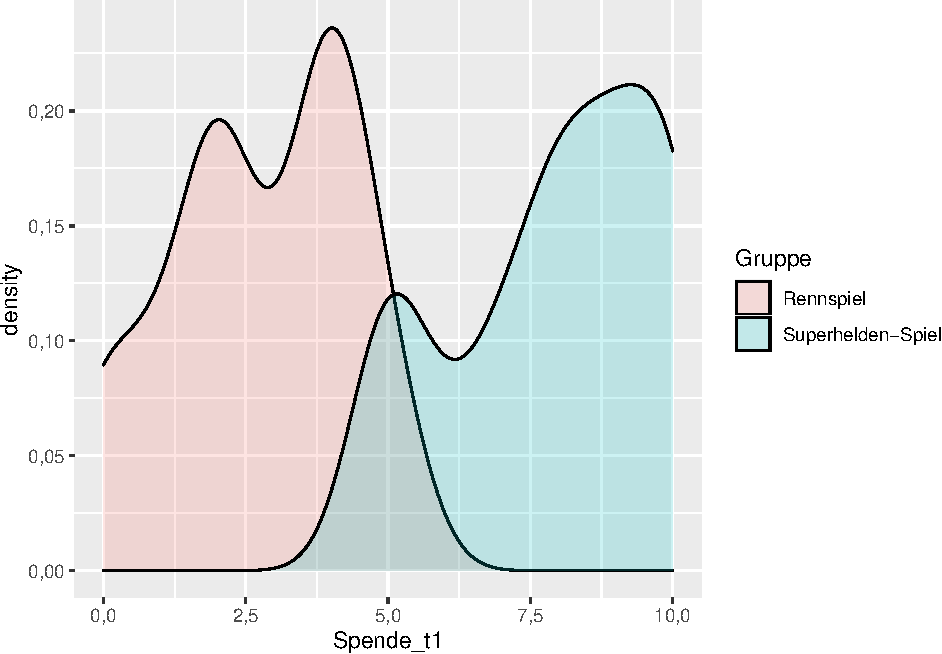
\includegraphics{r_book_files/figure-latex/unnamed-chunk-102-1.pdf}

\hypertarget{anwendungsvoraussetzungen}{%
\subsection{Anwendungsvoraussetzungen}\label{anwendungsvoraussetzungen}}

Wichtig bei Hypothesen für den T-Test für unabhängige Stichproben ist, dass -- wie der Name schon sagt -- die \textbf{Anwendungsvoraussetzung der Unabhängigkeit} erfüllt ist. Das bedeutet, dass die jeweils zu vergleichenden Populationen wirklich völlig random und unabhängig voneinander entstanden sein müssen. Im Hypothesen-Beispiel 1 werden Männer und Frauen untersucht, die nichts miteinander zu tun haben, also nicht z. B. verheiratet sind. -- Das wäre dann eine abhängige Stichprobe (siehe unten). Die Antworten eines jeden Mannes in der Stichprobe hängt dann überhaupt nicht davon ab, was irgendeine Frau im Sample sagt.

Hier ein Beispiel in dem die Unabhängigkeit nicht gegeben wäre: Bei verheirateten Paaren müsste man davon ausgehen, dass die Ehepartner sich gegenseitig in ihrem Politikinteresse annähern. Wenn der Mann einen sehr hohen Wert nennt, wäre davon auszugehen, dass der Wert der Frau ebenfalls hoch ist, z. B. weil beide häufig gemeinsam über Politik reden.

Die Anwendungsvoraussetzung der Intervallskalierung gilt natürlich weiterhin, wie schon für den Einstichproben-T-Test. -- Jedoch natürlich nur für die abhängige Variable, für die die Mittelwerte berechnet werden sollen.

Eine weitere Anwendungsvoraussetzung ist die \textbf{Varianzhomogenität / Homoskedastizität}: Die Varianzen müssen in den zu vergleichenden Teilpopulationen annäherungsweise gleich sein. Also ganz wörtlich: Ist in Population 1 die Varianz s² = 1,23 dann möchte man hier, dass Population 2 eben auch eine Varianz von s² = 1,23 aufweist oder einen Wert, der jedenfalls nicht signifikant davon abweicht.

Und wie testet man, ob die Kennwerte in zwei Stichproben sich signifikant von einander unterschieden? Das klingt ja fast wie der T-Test für unabhängige Stichproben, den wir ja ohnehin gerade hier behandeln! Tatsächlich ist es aber kein T-Test, der dabei angewendet wird, sondern ein F-Test. Der F-Test ist eine ganz ähnliche Teststatistik, die später bei den Varianzanalysen nochmal auftauchen wird.

Verrückt, oder? Bevor wir jetzt also einen T-Test für unsere unabhängigen Mittelwerte machen können, müssen wir erstmal einen genauso aufwendigen F-Test für die Varianzen machen, um die Anwendungsvoraussetzung zu prüfen. -- Aber dieser F-Test sollte nach Möglichkeit besser nicht signifikant werden, denn signifikant würde hier bedeuten, dass die beiden Varianzen sich unterscheiden. -- Und wir wollen schließlich Varianz\emph{homogenität}, also gleiche Varianzen. Der F-Test für die Varianzhomogenität hat einen speziellen Namen, er heißt Levene-Test (nach Howard Levene).

\leavevmode\hypertarget{danger_levene}{}%
\textbf{Levene: p \textless{} .05 = blöd, weil keine Varianzhomogenität!}

Als Studentin fand ich den Levene-Test super verwirrend, weil ich gerade gelernt hatte, dass winzig kleine p-Werte prima sind und für die aufgestellten Hypothesen sprechen. Und beim Levene-Test war auf einmal alles anders herum?! Das geht wirklich schwer in den Kopf rein und ich merke heute, dass nach wie vor viele Studierende damit Schwierigkeiten haben.

Um es nochmal ganz deutlich zu sagen: Normalerweise wollen wir ja, dass unsere Hypothesentests Unterschiede produzieren, damit wir uns gegen die Nullhypothese entscheiden können (die Nullhypothese sagt ja immer, dass es keinen Unterschied oder Zusammenhang gibt). Beim Levene-Test wollen wir hingegen, möglichst das hinsichtlich des Kriteriums der Varianz kein Unterschied besteht, damit die Gruppen hier vergleichbar sind. Der Levene-Test, testet lediglich die Varianz. Dass der Mittelwertunterschied signifikant ist, hoffen wir natürlich nach wie vor, das testen wir aber erst im Anschluss.

\hypertarget{levene-test-auf-varianzhomogenituxe4t}{%
\subsection{Levene-Test auf Varianzhomogenität}\label{levene-test-auf-varianzhomogenituxe4t}}

Also, auf geht`s, hier kommt der Levene-Test für die Daten und die Hypothese zur Spendenbereitschaft nach dem Spielen verschiedener Videospiel-Typen. Die \emph{Gruppe} ist die uV und die Variable \emph{Spende\_t01} die aV.

Für den Levene-Test benutze ich ebenfalls das Paket \texttt{rstatix} und die Funktion \texttt{levene\_test()}. Natürlich gibt es auch andere Pakete mit denen man Levene-Tests und T-Tests berechnen kann (z. B. \texttt{car}). \texttt{rstatix} bietet aber weiterhin den Vorteil, dass es ``pipeable'' ist.

Die Funktion hat folgende Argumente:

\begin{itemize}
\item
  Das erste Argument ist wieder das Datensatz-Objekt.
\item
  Das zweite ist eine Formel (wie bei der \protect\hyperlink{regression}{Regression}), die die Variablen der Analyse mit einer Tilde \texttt{\textasciitilde{}} verbindet. Die Tilde bedeutet dabei übersetzt in Worte etwa folgendes: ``Variable vor der Tilde wird vorhergesagt durch Variable nach der Tilde''. Die Notation ist immer \texttt{aV\ \textasciitilde{}\ uV}.
\item
  Außerdem kann man noch mit dem Argument \texttt{center\ =} die Art des Tests auswählen. Der Orginal-Levene-Test wird durch \texttt{center\ =\ "mean"} berechnet (so berechnet ihn auch das Programm SPSS standardmäßig). Allerdings haben \citep{Brown_1974} gezeigt, dass für schiefe Verteilungen der Variablen der Vergleich der Median einen besseren Hinweis auf die Homo- beziehungsweise Heterogenität der Varianzen gibt. Die Option \texttt{center\ =\ "median"} ist deshalb die Default-Option der \texttt{levene\_test()}- Funktion. Sie muss nicht gesondert eingestellt werden.
\end{itemize}

Angewendet sieht das so aus:

\begin{Shaded}
\begin{Highlighting}[]
\NormalTok{df\_prosocial }\SpecialCharTok{\%\textgreater{}\%} 
  \FunctionTok{levene\_test}\NormalTok{(Spende\_t1 }\SpecialCharTok{\textasciitilde{}}\NormalTok{ Gruppe)}
\end{Highlighting}
\end{Shaded}

\begin{verbatim}
## # A tibble: 1 x 4
##     df1   df2 statistic     p
##   <int> <int>     <dbl> <dbl>
## 1     1    66     0.156 0.695
\end{verbatim}

Prima, sehr schön! Ausgegeben wird unter ``statistic'' ein relativ kleiner F-Wert inklusive Freiheitsgraden (df1 und df2) und einem zugehörigen p-Wert. Dieser p-Wert ist größer als .05, also nicht signifikant. Es spricht also alles dafür, dass die Varianzen der Variable \emph{Spenden\_t1} in beiden Teil-Stichproben (Gruppe Superhelden und Gruppe Rennspiel) gleich sind. Dem nun folgenden T-Test steht also nichts entgegen.

\leavevmode\hypertarget{info_varianzhetero}{}%
\textbf{Was, wenn der Levene-Test doch signifikant wird?}

Dann wären die Varianzen nicht gleich/homogen. Das wäre für den Standard-T-Test schlecht, ist aber praktisch nicht so schlimm, denn den T-Test gibt es auch in einer robusten Variante (Welch-Korrektur), bei der die Prüfgröße T und ihr Signifikanztest korrigiert werden -- und zwar in dem Maße in dem die Varianzen ungleich sind.

\hypertarget{t-test-durchfuxfchren-1}{%
\subsection{T-Test durchführen}\label{t-test-durchfuxfchren-1}}

Den T-Test für unabhängige Stichproben erhält man in R ebenfalls über das \texttt{rstatix}-Paket und die \texttt{t\_test()}-Funktion. Hier die relevanten Argumente:

\begin{enumerate}
\def\labelenumi{\arabic{enumi}.}
\item
  Datensatz-Objekt
\item
  Das zweite Argument ist wieder die Formel, mit \texttt{aV\ \textasciitilde{}\ uV}.
\item
  Standardmäßig geht die Funktion \texttt{t\_test()} davon aus, dass die Varianzen \textbf{nicht} gleich sind (entspricht \texttt{var.equal\ =\ FALSE}). In unserem Fall haben wir aber sogar vorab auf gleiche Varianzen getestet und können durch \texttt{var.equal\ =\ TRUE} einen Test ohne Korrektur anfordern. Es empfiehlt sich, immer einen Levene-Test vorzuschalten und das \texttt{var.equal}-Argument bewusst auf \texttt{TRUE}oder \texttt{FALSE} zu setzen.
\item
  Mit \texttt{alternative} kann man festlegen, ob der Test ungerichtet (\texttt{"two.sided"}) oder einseitig (\texttt{"less"} oder \texttt{"greater"}) stattfinden soll.
\item
  Mit \texttt{detailed\ =\ TRUE} bzw. \texttt{FALSE} kann man wieder über den Detailgrad der Ausgabe bestimmen.
\end{enumerate}

Hier der Test der H2:

\begin{Shaded}
\begin{Highlighting}[]
\NormalTok{df\_prosocial }\SpecialCharTok{\%\textgreater{}\%} 
  \FunctionTok{t\_test}\NormalTok{(Spende\_t1 }\SpecialCharTok{\textasciitilde{}}\NormalTok{ Gruppe, }\AttributeTok{var.equal =} \ConstantTok{TRUE}\NormalTok{, }\AttributeTok{alternative =} \StringTok{"less"}\NormalTok{) }
\end{Highlighting}
\end{Shaded}

\begin{verbatim}
## # A tibble: 1 x 8
##   .y.       group1    group2               n1    n2 statistic    df        p
## * <chr>     <chr>     <chr>             <int> <int>     <dbl> <dbl>    <dbl>
## 1 Spende_t1 Rennspiel Superhelden-Spiel    35    35     -12.6    66 1.51e-19
\end{verbatim}

Das Ergebnis sieht so ähnlich aus wie vorhin, beim ersten T-Test. Es gibt wieder einen t-Wert unter ``statistic'', entsprechende Freiheitsgrade und einen zugehörigen p-Wert. Dieser ist deutlich \textless{} .05, das Ergebnis ist also signifikant, was für die Alternativhypothese spricht. Die Grenzen des Konfidenzintervalls können über die detaillierte Ausgabe mit \texttt{detailed\ =\ TRUE} angefordert werden (aus Platzgründen nicht dargestellt). Diesen Grenzen zur Folge würden wir die Mittelwertdifferenz zwischen \text{-5,96} und \text{-4,33} schätzen. Das ist beides deutlich von Null verschieden (anders ausgedrückt: Die Grenzen schließen die Null nicht ein).

Beide Grenzen der Konfidenzintervalle sind außerdem negativ. Der Grund dafür ist, dass die Ausprägung Rennspiel in der uV mit einer kleineren Ordnungsnummer codiert wurde und deshalb zuerst in die Auswertung einging und natürlich, dass ihr Mittelwert auch kleiner ist als der der Ausprägung Superhelden. Das Vorzeichen hat in diesem Fall jedoch keine sinnvoll zu interpretierende Bedeutung, weil die uV nominal ist (es gibt keine ``Reihenfolge'' zwischen Superheldenspiel und Rennspiel).

Das Ergebnis des T-Tests zeigt, dass das die Spieler:innen, die das Superheldenspiel gespielt haben, deutlich spendabler waren als die Spieler:innen des Rennspiels. Erstere spendeten im Durchschnitt M = \text{7,91} Euro, letztere nur M = \text{2,76} Euro. Das Ergebnis des T-Tests für unabhängige Stichproben fiel im Sinne von H2 aus und ist mit t(\text{66}) = \text{-5,15} auf dem Niveau p \textless{} ,001 signifikant. Offensichtlich hat das Spielen eines Superheldenspiels tatsächlich einen positiven Einfluss auf das prosoziale Verhalten, wie hier am Beispiel der Spendenbereitschaft demonstriert wurde (hier wurden jedoch keine echten Daten analysiert).

\hypertarget{cohens-d-1}{%
\subsection{Cohen´s d}\label{cohens-d-1}}

Ergänzend kann auch beim T-Test für unabhängige Stichproben die Effektstärke Cohen´s d berechnet werden:

\begin{Shaded}
\begin{Highlighting}[]
\NormalTok{df\_prosocial }\SpecialCharTok{\%\textgreater{}\%} 
  \FunctionTok{cohens\_d}\NormalTok{(Spende\_t1 }\SpecialCharTok{\textasciitilde{}}\NormalTok{ Gruppe, }\AttributeTok{var.equal =} \ConstantTok{TRUE}\NormalTok{) }
\end{Highlighting}
\end{Shaded}

\begin{verbatim}
## # A tibble: 1 x 7
##   .y.       group1    group2            effsize    n1    n2 magnitude
## * <chr>     <chr>     <chr>               <dbl> <int> <int> <ord>    
## 1 Spende_t1 Rennspiel Superhelden-Spiel   -3.06    35    35 large
\end{verbatim}

\begin{Shaded}
\begin{Highlighting}[]
\NormalTok{cd }\OtherTok{\textless{}{-}}\NormalTok{ df\_prosocial }\SpecialCharTok{\%\textgreater{}\%} 
  \FunctionTok{cohens\_d}\NormalTok{(Spende\_t1 }\SpecialCharTok{\textasciitilde{}}\NormalTok{ Gruppe, }\AttributeTok{var.equal =} \ConstantTok{TRUE}\NormalTok{) }
\end{Highlighting}
\end{Shaded}

Die Interpretation des T-Tests kann um einen entsprechenden Satz ergänzt werden: Der gefundene Effekt ist mit Cohen´s d = \text{-3,06} als stark zu bezeichnen.

\hypertarget{t-test-fuxfcr-abhuxe4ngige-stichproben}{%
\section{T-Test für abhängige Stichproben}\label{t-test-fuxfcr-abhuxe4ngige-stichproben}}

Im vorigen Abschnitt wurde der T-Test für unabhängige Stichproben erläutert. Dabei spielten zwei Variablen eine Rolle die unterschiedliches Datenniveau hatten: Es gab eine nominale uV mit der zwei Gruppen gebildet wurden und eine (quasi-)metrisch skalierte aV, deren Mittelwert berechnet wurde (2x). Beim T-Test für \textbf{abhängige Stichproben} sieht es anders aus: Hier werden \emph{zwei prinzipiell gleich aufgebaute Variablen} mit einander verglichen:

\begin{itemize}
\item
  Beide sollen (quasi-)metrisches Datenniveau aufweisen.
\item
  Beide sollen auf der gleichen Skala gemessen worden sein und theoretisch den gleichen Wertebereich aufweisen (also z. B. beide von 1 = \emph{stimme überhaupt nicht zu} bis 5 = \emph{stimme voll und ganz zu} gemessen worden sein. Wenn in einer Variable eine Ausprägung empirisch nicht vorkommt, also z. B. niemand 5 = \emph{stimme voll und ganz zu} angekreuzt hat, ist es aber trotzdem okay, die Variable zu verwenden).
\item
  Wie der Name des Tests schon sagt, müssen außerdem die Stichproben abhängig sein. Das bedeutet, dass die Variablen als zwei getrennte Variablen im Datensatz vorliegen, jedenfalls sofern er ``wide format'' aufweist. Für jeden Fall im Datensatz wurde ein Wert in Variable 1 und ein Wert in Variable 2 gemessen (tendenziell, ein paar fehlende Messwerte sind okay).
\end{itemize}

Nun wieder ein paar Beispiele für Fragestellungen, die man mit dem T-Test für abhängige Stichproben prüfen kann:

\begin{itemize}
\item
  Unterscheiden sich die Mittelwerte von zwei Items einer Skala voneinander?
\item
  Welcher Wert ist höher, der für Zustimmung zum Item ``Die Klimakrise ist das wichtigste Problem unserer Zeit'' oder zu ``Soziale Gerechtigkeit ist das wichtigste Problem unserer Zeit''?
\item
  Unterschiedet sich das politische Interesse von Ehefrauen von dem ihrer Ehemänner?
\item
  Unterscheidet sich eine bestimmte Variable im Zeitverlauf zu unterschiedlichen Messzeitpunkten (z.B. (1) vor und nach Gabe eines Treatments und danach oder (2) direkt nach dem Experiment und eine Woche später).
\end{itemize}

Im Anwendungsbeispiel möchten wir nun prüfen, ob der positive Effekt, den wir für das Spielen von Superhelden-Spielen gefunden haben, auch über längere Zeit anhält, oder nicht. Theoretisch ist davon auszugehen, dass das einmalige Spielen eines Superhelden-Spiels das prosoziale Verhalten zwar kurzfristig, aber nicht über einen längeren Zeitraum hinweg verändern kann. Deshalb lautet die zu testende Hypothese:

\emph{H3a: Die Spendenbereitschaft der Superhelden-Spieler:innen ist zum Zeitpunkt T2 niedriger als zum Zeitpunkt T1.}

Für die Gruppe der Rennspiel-Spieler:innen würde man natürlich so einen Effekt nicht erwarten. Hier sollte das Niveau gleichbleibend niedrig sein. Eine Hypothese, die keinen Effekt voraussagt, wäre eine Nullhypothese. Eine Nullhypothese kann mit der Inferenzstatistik nicht verifiziert sondern nur widerlegt werden. Der Vollständigkeit halber stellen wir deshalb die zugehörige Alternativhypothese auf, obwohl wir nicht erwarten, dass sie sich bestätigen lässt:

\emph{H3b: Die Spendenbereitschaft der Rennspiel-Spieler:innen unterschiedet sich an beiden Messzeitpunkten.}

Während H3a eine gerichtete Hypothese ist, ist H3b ungerichtet, denn es besteht kein Argument für die Formulierung einer Richtung.

\hypertarget{deskriptiver-vergleich}{%
\subsection{Deskriptiver Vergleich}\label{deskriptiver-vergleich}}

Natürlich bietet es sich auch vor dem T-Test für abhängige Stichproben an, zunächst deskriptiv zu evaluieren, wie die Variablen verteilt sind und wo die Mittelwerte liegen. Auch hier werden zunächst grafische Analysen genutzt. Mit dem Befehl \texttt{facet\_wrap()} kann man die Darstellung für die Gruppen aufteilen:

\begin{Shaded}
\begin{Highlighting}[]
\NormalTok{df\_prosocial }\SpecialCharTok{\%\textgreater{}\%} 
  \FunctionTok{ggplot}\NormalTok{() }\SpecialCharTok{+}
  \FunctionTok{geom\_density}\NormalTok{(}\FunctionTok{aes}\NormalTok{(Spende\_t1), }\AttributeTok{alpha =} \FloatTok{0.2}\NormalTok{, }\AttributeTok{fill =} \StringTok{"blue"}\NormalTok{) }\SpecialCharTok{+}
  \FunctionTok{geom\_density}\NormalTok{(}\FunctionTok{aes}\NormalTok{(Spende\_t2), }\AttributeTok{alpha =} \FloatTok{0.2}\NormalTok{, }\AttributeTok{fill =} \StringTok{"orange"}\NormalTok{) }\SpecialCharTok{+}
  \FunctionTok{facet\_wrap}\NormalTok{(}\SpecialCharTok{\textasciitilde{}}\NormalTok{Gruppe)}
\end{Highlighting}
\end{Shaded}

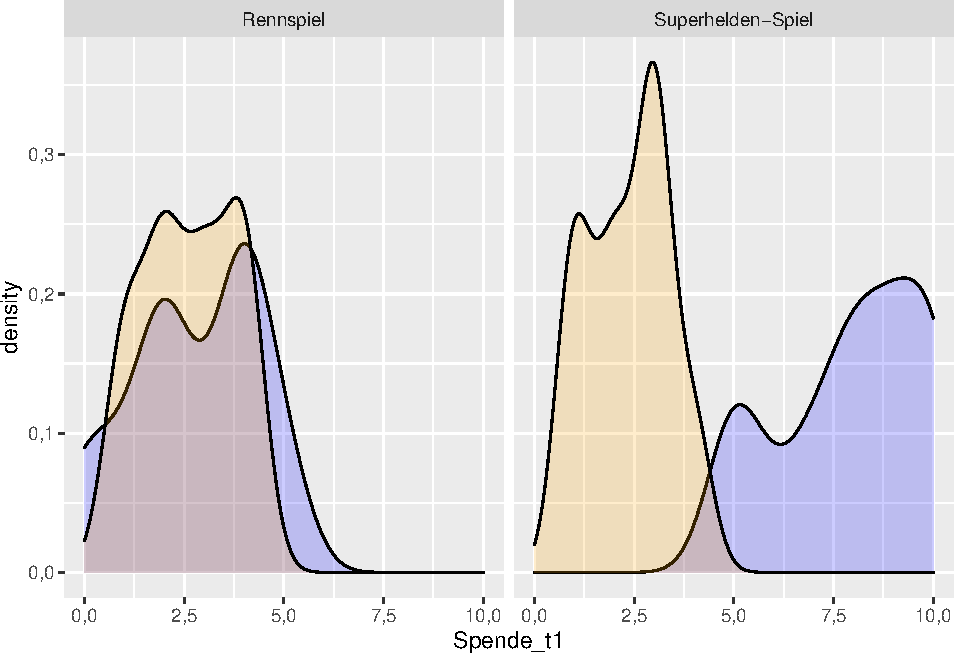
\includegraphics{r_book_files/figure-latex/unnamed-chunk-108-1.pdf}

Die Verteilungen sind deutlich unterschiedlich für die beiden Gruppen. Während bei den Rennspielen die Werte zu beiden Zeitpunkten in einem ähnlichen Spektrum liegen, ist dies bei den Superhelden-Spielen nicht der Fall. Die Superhelden-Gruppe ist ja auch genau die Gruppe, die im Rahmen von von H3a interessiert. Es sieht gut aus für die Vermutung, dass es in der Gruppe der Superhelden-Spieler:innen einen signifikanten Mittelwertunterschied zwischen den beiden Messzeitpunkten Spende\_t01 und Spende\_t02 gibt -- und in der Gruppe Rennspiele (H3b) wie erwartet nicht.

Die Mittelwertunterschiede kann man natürlich nicht nur grafisch, sondern auch in Zahlen ausdrücken. Ich nutze hier das tidyverse um eine gruppierte Darstellung (aufgeteilt nach Gruppe) zu erzeugen:

\begin{Shaded}
\begin{Highlighting}[]
\NormalTok{mw\_table }\OtherTok{\textless{}{-}}\NormalTok{ df\_prosocial }\SpecialCharTok{\%\textgreater{}\%} 
  \FunctionTok{select}\NormalTok{(Gruppe, Spende\_t1, Spende\_t2) }\SpecialCharTok{\%\textgreater{}\%} 
  \FunctionTok{group\_by}\NormalTok{(Gruppe) }\SpecialCharTok{\%\textgreater{}\%} 
  \FunctionTok{summarise}\NormalTok{(}\AttributeTok{t1\_M =} \FunctionTok{mean}\NormalTok{(Spende\_t1, }\AttributeTok{na.rm=} \ConstantTok{TRUE}\NormalTok{),}
            \AttributeTok{t1\_SD =} \FunctionTok{SD}\NormalTok{(Spende\_t1, }\AttributeTok{na.rm=} \ConstantTok{TRUE}\NormalTok{),}
            \AttributeTok{t1\_n =} \FunctionTok{n}\NormalTok{(),}
            \AttributeTok{t2\_M =} \FunctionTok{mean}\NormalTok{(Spende\_t2, }\AttributeTok{na.rm=} \ConstantTok{TRUE}\NormalTok{),}
            \AttributeTok{t2\_SD =} \FunctionTok{SD}\NormalTok{(Spende\_t2, }\AttributeTok{na.rm=} \ConstantTok{TRUE}\NormalTok{),}
            \AttributeTok{t2\_n =} \FunctionTok{n}\NormalTok{())}

\NormalTok{mw\_table}
\end{Highlighting}
\end{Shaded}

\begin{verbatim}
## # A tibble: 2 x 7
##   Gruppe             t1_M t1_SD  t1_n  t2_M t2_SD  t2_n
##   <chr>             <dbl> <dbl> <int> <dbl> <dbl> <int>
## 1 Rennspiel          2.76  1.58    35  2.62  1.13    35
## 2 Superhelden-Spiel  7.91  1.78    35  2.35  1.01    35
\end{verbatim}

Anders als beim T-Test für unabhängige Stichproben vergleicht man bei der Betrachtung für den T-Test für abhängige Stichproben die Mittelwerte in einer Zeile in den unterschiedlichen Spalten. Für die Zeile ``Rennspiel'' (H3b) ergibt sich hier kaum ein Unterschied (2.76470588235294 gegenüber 2.61764705882353). Für die Zeile ``Superhelden-Spiel'' (H3a) ergibt sich jedoch ein deutlicher Unterschied (7.91176470588235 gegenüber 2.35294117647059). Nun wäre es wichtig zu wissen, ob die Mittelwertunterschiede signifikant sind.

\hypertarget{levene-tests-durchfuxfchren}{%
\subsection{Levene-Tests durchführen}\label{levene-tests-durchfuxfchren}}

Natürlich brauchen wir vor dem T-Tet wieder einen Levene-Test. Um diesen Test durchführen zu können, muss der Datensatz vom ``wide-format'' in ein ``long-format'' überführt werden (vgl. dazu Abschnitt {[}Datenumformungen{]}). Da die \texttt{levene\_test()}-Funktion tidy ist, kann man die Umformung einfach in der Pipe vor den Test schalten. Und noch etwas kann man davorschalten: Eine Aufteilung in die Gruppen, so dass der Levene-Test getrennt für beide Experimentalgruppen ausgegeben werden kann.

\begin{Shaded}
\begin{Highlighting}[]
\NormalTok{df\_prosocial }\SpecialCharTok{\%\textgreater{}\%}
  \FunctionTok{pivot\_longer}\NormalTok{(}\AttributeTok{cols =} \FunctionTok{c}\NormalTok{(Spende\_t1, Spende\_t2), }
               \AttributeTok{names\_to =} \StringTok{"Zeitpunkt"}\NormalTok{, }
               \AttributeTok{values\_to =} \StringTok{"Betrag"}\NormalTok{) }\SpecialCharTok{\%\textgreater{}\%} 
  \FunctionTok{group\_by}\NormalTok{(Gruppe) }\SpecialCharTok{\%\textgreater{}\%} 
  \FunctionTok{levene\_test}\NormalTok{(Betrag }\SpecialCharTok{\textasciitilde{}}\NormalTok{ Zeitpunkt)}
\end{Highlighting}
\end{Shaded}

\begin{verbatim}
## # A tibble: 2 x 5
##   Gruppe              df1   df2 statistic       p
##   <chr>             <int> <int>     <dbl>   <dbl>
## 1 Rennspiel             1    66      4.47 0.0384 
## 2 Superhelden-Spiel     1    66      8.26 0.00544
\end{verbatim}

Das Ergebnis zeigt sich signifikant für beide Gruppen, denn p ist jeweils \textless{} .05. Wir können also nicht von Varianzhomogenität ausgehen und müssen für den folgenden T-Test merken, dass der korrigierte Test benötigt wird.

\hypertarget{t-test-durchfuxfchren-2}{%
\subsection{T-Test durchführen}\label{t-test-durchfuxfchren-2}}

Der T-Test für abhängige Stichproben benötigt dieselbe Datenumformung in das ``long-format'' wie der Levene-Test. Auch hier können wir diese wieder in der Pipe davor schalten und ebenso auch die Aufteilung in beide Gruppen. Die einfachste Variante den T-Test anzufordern ist über die bereits bekannte \texttt{t-test()}- Funktion. Benötigt wird allerdings das zusätzliche Argument \texttt{paired\ =\ TRUE}, damit der paarweise Test durchgeführt wird. Außerdem setzen wir explizit \texttt{var.equal\ =\ FALSE}, weil der Levene-Test ein signifikantes Ergebnis produziert hat und deshalb nicht von Varianzhomogenität ausgegangen werden kann. Ich belasse es an dieser Stelle bei der Default-Einstellung \texttt{alternative\ =\ "two.sided"}, da ich eine gerichtete und eine ungerichtete Hypothese gleichzeitig prüfen möchte und der zweiseitige Test der strengere ist. Theoretisch würde für H3a aber ein einseitiger Test ausreichen.

\begin{Shaded}
\begin{Highlighting}[]
\NormalTok{df\_prosocial }\SpecialCharTok{\%\textgreater{}\%}
        \FunctionTok{pivot\_longer}\NormalTok{(}\AttributeTok{cols =} \FunctionTok{c}\NormalTok{(Spende\_t1, Spende\_t2), }
                     \AttributeTok{names\_to =} \StringTok{"Zeitpunkt"}\NormalTok{, }
                     \AttributeTok{values\_to =} \StringTok{"Betrag"}\NormalTok{) }\SpecialCharTok{\%\textgreater{}\%} 
        \FunctionTok{group\_by}\NormalTok{(Gruppe) }\SpecialCharTok{\%\textgreater{}\%} 
        \FunctionTok{t\_test}\NormalTok{(Betrag }\SpecialCharTok{\textasciitilde{}}\NormalTok{ Zeitpunkt, }
               \AttributeTok{var.equal =} \ConstantTok{FALSE}\NormalTok{, }
               \AttributeTok{paired =} \ConstantTok{TRUE}\NormalTok{,}
               \AttributeTok{alternative =} \StringTok{"two.sided"}\NormalTok{)}
\end{Highlighting}
\end{Shaded}

\begin{verbatim}
## # A tibble: 2 x 9
##   Gruppe           .y.    group1   group2      n1    n2 statistic    df        p
## * <chr>            <chr>  <chr>    <chr>    <int> <int>     <dbl> <dbl>    <dbl>
## 1 Rennspiel        Betrag Spende_~ Spende_~    35    35     0.457    32 6.51e- 1
## 2 Superhelden-Spi~ Betrag Spende_~ Spende_~    35    35    14.9      32 5.52e-16
\end{verbatim}

Der Output enthält in den beiden Zeilen zwei T-Tests für abhängige Stichproben, oben für H3b und unten für H3a. In der Spalte ``estimate'' sind die Werte der Mittelwertdiffrenzen angegeben.

\textbf{Interpretation H3b (erste Zeile):}

In der Gruppe ``Rennspiel'' beträgt die Mittelwertdifferenz nur c(\texttt{mean\ of\ the\ differences} = 0.151515151515152) Euro. Der T-Wert ist mit T(c(df = 32)) = c(t = 0.456673377277543) sehr klein. Der p-Wert sieht zwar wegen der ``wissenschaftlichen'' Notation kompliziert aus, aber lassen Sie sich davon nicht in die Irre führen! Er ist recht hoch: p = 0.651 und damit nicht signifikant. Insgesamt muss die H3b deshalb abgelehnt werden. Wie erwartet.

\begin{Shaded}
\begin{Highlighting}[]
\NormalTok{sn }\OtherTok{\textless{}{-}} \FunctionTok{case\_when}\NormalTok{(tt\_pairwise[[}\DecValTok{2}\NormalTok{, }\StringTok{"p"}\NormalTok{]] }\SpecialCharTok{\textless{}} \FloatTok{0.001} \SpecialCharTok{\textasciitilde{}} \StringTok{"p \textless{} ,001"}\NormalTok{,}
\NormalTok{                tt\_pairwise[[}\DecValTok{2}\NormalTok{, }\StringTok{"p"}\NormalTok{]] }\SpecialCharTok{\textless{}} \FloatTok{0.01} \SpecialCharTok{\textasciitilde{}} \StringTok{"p \textless{} ,01"}\NormalTok{,}
\NormalTok{                tt\_pairwise[[}\DecValTok{2}\NormalTok{, }\StringTok{"p"}\NormalTok{]] }\SpecialCharTok{\textless{}} \FloatTok{0.05} \SpecialCharTok{\textasciitilde{}} \StringTok{"\textless{} ,05"}\NormalTok{,}
                \ConstantTok{TRUE} \SpecialCharTok{\textasciitilde{}} \StringTok{"n.s."}\NormalTok{)}
\end{Highlighting}
\end{Shaded}

** Interpretation H3a (zweite Zeile):**

In der Gruppe ``Superhelden'' beträgt die Mittelwertdifferenz hingegen stolze c(\texttt{mean\ of\ the\ differences} = 5.48484848484848) Euro (zur Erinnerung, die Proband:innen hatten maximal 10 Euro zur Verfügung). Die T-Statistik ist mit T(c(df = 32)) = c(t = 14.9445217485871) auf dem Niveau p \textless{} ,001 signifikant. Dieses Daten sprechen für H3a, die entsprechende Nullhypothese wird zurückgewiesen.

\hypertarget{cohens-d-2}{%
\subsection{Cohen´s d}\label{cohens-d-2}}

Selbstredend kann auch hier wieder Cohen´s d berechnet werden, um die Effektstärke einzuordnen. Dabei wird ebenfalls die gesamte Pipe vorgeschaltet und die Angaben zur Varianzheterogenität und dass es sich um einen T-Test für abhängige Stichproben handelt dürfen auch in der \texttt{cohens\_d()}-Funktion nicht fehlen.

\begin{Shaded}
\begin{Highlighting}[]
\NormalTok{df\_prosocial }\SpecialCharTok{\%\textgreater{}\%}
      \FunctionTok{pivot\_longer}\NormalTok{(}\AttributeTok{cols =} \FunctionTok{c}\NormalTok{(Spende\_t1, Spende\_t2), }
                   \AttributeTok{names\_to =} \StringTok{"Zeitpunkt"}\NormalTok{, }
                   \AttributeTok{values\_to =} \StringTok{"Betrag"}\NormalTok{) }\SpecialCharTok{\%\textgreater{}\%} 
      \FunctionTok{group\_by}\NormalTok{(Gruppe) }\SpecialCharTok{\%\textgreater{}\%} 
      \FunctionTok{cohens\_d}\NormalTok{(Betrag }\SpecialCharTok{\textasciitilde{}}\NormalTok{ Zeitpunkt, }
             \AttributeTok{var.equal =} \ConstantTok{FALSE}\NormalTok{, }
             \AttributeTok{paired =} \ConstantTok{TRUE}\NormalTok{) }
\end{Highlighting}
\end{Shaded}

\begin{verbatim}
## # A tibble: 2 x 8
##   .y.    group1    group2    effsize Gruppe               n1    n2 magnitude 
## * <chr>  <chr>     <chr>       <dbl> <chr>             <int> <int> <ord>     
## 1 Betrag Spende_t1 Spende_t2  0.0795 Rennspiel            35    35 negligible
## 2 Betrag Spende_t1 Spende_t2  2.60   Superhelden-Spiel    35    35 large
\end{verbatim}

Wie zu erwarten war, ist die Effektstärke für H3b verschwindend gering -- der Signifikanztest zeigte ja ohnehin ein negatives Ergebnis. Für H3a enthüllt Cohen´s d jedoch einen starken Effekt.

\hypertarget{varianzanalyse}{%
\chapter{Varianzanalyse}\label{varianzanalyse}}

\emph{Die Erarbeitung dieses Kapitels erfolgte auf Basis eines Skripts, welches Daniel Possler 2021 für die Veranstaltung SDA2 erstellt hat. Dieser wiederum nutzte Vorarbeiten von Jule Scheper, Sophie Bruns und Anna Freytag.}

Im letzten Kapitel haben wir mit dem T-Test ein Verfahren kennengelernt, mit dem wir Unterschiedshypothesen prüfen können, indem die Mittelwerte von zwei Gruppen verglichen werden. Was aber, wenn wir nicht zwei sondern mehr Gruppen haben? Hier kommt die Varianzanalyse ins Spiel. Mit der Varianzanalyse (englisch ANOVA = \textbf{an}alysis \textbf{o}f \textbf{va}riance) ist dies möglich. Genau wie der im letzten Kapitel angewendete T-Test hat die abhängige Variable der Varianzanalyse metrisches Datenniveau und die unabhängige mindestens nominales\footnote{Selbstverständlich ist auch ein höheres Datenniveau möglich. Wegen der Stichprobengröße in den einzelnen Gruppen und der Übersichtlichkeit sollte die unabhängige Variable aber nicht sehr viele Ausprägungen haben, weshalb metrische Variablen kaum als Faktoren in der Varianzanalyse eingesetzt werden.}. Ein Unterschied ist, dass die unabhängige Variable mehr als zwei Ausprägungen haben darf. -- Sie muss also nicht zwingend dichotom sein. Ein anderer Unterschied ist, dass als Prüfgröße nicht die T-Verteilung verwendet wird, sondern die von Ronald a. Fisher entwickelte F-Verteilung. Die Prüfgröße heißt deshalb \emph{F}.

Mit der Varianzanalyse können auch komplexe experimentelle Designs ausgewertet werden, bei denen es z. B. mehr als ein Einflussfaktor berücksichtigt wird. Nimmt man nur einen Einflussfaktor auf, handelt es sich um eine \emph{einfaktorielle} Varianzanalyse (One-way Anova), bei zwei Faktoren spricht man von einer \emph{zweifaktoriellen} Varianzanalyse (Two-way Anova) und bei noch mehr Faktoren von einer mehrfaktoriellen Varianzanalyse.

\hypertarget{datenbeispiel-1}{%
\section{Datenbeispiel}\label{datenbeispiel-1}}

Die Daten für dieses Kapitel liefert die BA-Arbeit von Carsten Reichelt (2019). Vielen Dank an dieser Stelle! Carsten Reichelt hat in seiner BA-Arbeit untersucht, ob der Schwierigkeitsgrad eines Videospiels eine Rolle für die Performance und das Erleben von Unterhaltung der Spieler:innen spielt. Um diese Frage zu klären hat er ein Online-Experiment designed in dem N = 248 nutzten Proband:innen vier Minuten lang das Spiel Pac-Man spielen mussten (= Stimulus). Der Stimulus wurde dabei über die drei Schwierigkeitsgrade ``einfach'' (n = 79), ``mittel'' (n = 90) und schwer (n = 79) variiert. Die Gruppenzugehörigkeit bildet also die zentrale unabhängige Variable und sie ist dreistufig (einfach, mittel oder schwer). Nach dem Spielen füllten die Proband:innen einen Online-Fragebogen aus, in dem verschiedene weitere, abhängige und unabhängige Variablen erhoben wurden. Außerdem wurde der Highsore, den die Proband:innen erzielten erfasst.

\hypertarget{prerequisits}{%
\section{Prerequisits}\label{prerequisits}}

Zunächst benötigen wir natürlich verschiedene Pakete zur Durchfühung der Varianzanalyse:

\begin{Shaded}
\begin{Highlighting}[]
\FunctionTok{library}\NormalTok{(tidyverse) }\CommentTok{\# für Grafiken und die Pipe}
\FunctionTok{library}\NormalTok{(janitor)   }\CommentTok{\# für Häufigkeitsauszählungen}
\FunctionTok{library}\NormalTok{(rstatix)   }\CommentTok{\# für den Levene{-}Test}
\FunctionTok{library}\NormalTok{(effectsize)}\CommentTok{\# für Eta{-}Quadrat}
\FunctionTok{library}\NormalTok{(afex)      }\CommentTok{\# zur Berechnung der mehrfaktoriellen Anova}
\end{Highlighting}
\end{Shaded}

Die Die Daten der Abschlussarbeit von Herrn Reichelt liegen im SPSS-Format .sav. vor. Sie können über das Paket \texttt{haven} geladen werden. Da wir die unabhängigen Variablen für die Varianzanalyse in R als \emph{Faktoren} benötigen, wandeln wir diese gleich im Anschluss an den Ladevorgang direkt in das benötigte Format um.

\begin{Shaded}
\begin{Highlighting}[]
\NormalTok{df }\OtherTok{\textless{}{-}}\NormalTok{ haven}\SpecialCharTok{::}\FunctionTok{read\_sav}\NormalTok{(}\StringTok{"data/BA–Carsten Reichelt.sav"}\NormalTok{, }\AttributeTok{user\_na =} \ConstantTok{FALSE}\NormalTok{) }\SpecialCharTok{\%\textgreater{}\%} 
  \FunctionTok{mutate}\NormalTok{(}\AttributeTok{Schwierigkeitsgrad =} \FunctionTok{factor}\NormalTok{(Schwierigkeitsgrad, }
                                     \AttributeTok{labels =} \FunctionTok{c}\NormalTok{(}\StringTok{"einfach"}\NormalTok{, }\StringTok{"mittel"}\NormalTok{, }\StringTok{"schwer"}\NormalTok{), }
                                     \AttributeTok{ordered =} \ConstantTok{TRUE}\NormalTok{),}
         \AttributeTok{Wettkampfpraeferenz =} \FunctionTok{factor}\NormalTok{( v\_12\_rec,}
                                       \AttributeTok{labels =} \FunctionTok{c}\NormalTok{(}\StringTok{"geringe Wettkampfpräferenz"}\NormalTok{, }\StringTok{"hohe Wettkampfpräferenz"}\NormalTok{),}
                                       \AttributeTok{ordered =} \ConstantTok{TRUE}\NormalTok{)) }\SpecialCharTok{\%\textgreater{}\%} 
  \FunctionTok{select}\NormalTok{(lfdn, Schwierigkeitsgrad, Highscore, Wettkampfpraeferenz)}

\NormalTok{df}
\end{Highlighting}
\end{Shaded}

\begin{verbatim}
## # A tibble: 248 x 4
##     lfdn Schwierigkeitsgrad Highscore Wettkampfpraeferenz       
##    <dbl> <ord>                  <dbl> <ord>                     
##  1    91 mittel                  1950 hohe Wettkampfpräferenz   
##  2    92 einfach                 3890 geringe Wettkampfpräferenz
##  3    93 einfach                 5200 hohe Wettkampfpräferenz   
##  4    98 mittel                  3930 geringe Wettkampfpräferenz
##  5   104 schwer                  1660 geringe Wettkampfpräferenz
##  6   106 mittel                  3280 hohe Wettkampfpräferenz   
##  7   113 einfach                 9000 hohe Wettkampfpräferenz   
##  8   114 einfach                 7920 hohe Wettkampfpräferenz   
##  9   123 mittel                  4800 geringe Wettkampfpräferenz
## 10   135 einfach                 5520 geringe Wettkampfpräferenz
## # ... with 238 more rows
\end{verbatim}

\hypertarget{einfaktorielle-varianzanalyse}{%
\section{Einfaktorielle Varianzanalyse}\label{einfaktorielle-varianzanalyse}}

Bevor wir uns an komplexere Designs wagen, testen wir ersteinmal eine ganz basale Hypothese, die quasi Voraussetzung für die weiteren Analysen in der BA-Arbeit von Herrn Reichelt ist. Im Experiment wird davon ausgagangen, dass die Gruppenzuteilung und der in der jeweiligen Gruppe angewendete Stimulus ursächlich verantwortlich ist für die Varianz zwischen den Gruppen.

Die Hypothese, die zuerst betrachtet wird, ist quasi der Test, ob die Variation durch den Stimulus funktioniert hat (\emph{Treatmentcheck}). Es sollte so sein, dass der Schwierigkeitsgrad den High-Score beeinflusst, und zwar in ``gegenläufiger'' (anti-proportionaler) Richtung. Salopp gesagt: Je schwerer das Spiel, desto geringer der Highscore. Anders formuliert könnte die Hypothese so lauten:

\emph{H1: Der Schwierigkeitsgrad beeinflusst den erzielten Highscore negativ.}

\hypertarget{deskriptive-analyse}{%
\subsection{Deskriptive Analyse}\label{deskriptive-analyse}}

Bevor es an die tatsächliche Prüfung der aufgestellten Hypothese geht, empfiehlt es sie wie immer, sich mit den Mitteln der deskriptiven Statistik und mit Grafiken einen Überblick über die Datenlage zu verschaffen.

Schauen wir uns zunächst die Verteilung der abhängigen Variablen an. Da es sich um eine nominale Variable handelt, interessiert hier vor allem die Häufigkeitsverteilung (und nicht etwa Lage und Streuungsmaße). Zur Anzeige der Häufigkeitsberteilung gibt es viele Wege, etwa \texttt{table()}oder \texttt{summary()}. Damit ich hier auch die realtiven Häufigkeiten erhalte, nutze ich \texttt{tabyl()}aus dem \texttt{janitor}-Paket.

\begin{Shaded}
\begin{Highlighting}[]
\NormalTok{df }\SpecialCharTok{\%\textgreater{}\%} 
\NormalTok{  janitor}\SpecialCharTok{::}\FunctionTok{tabyl}\NormalTok{(Schwierigkeitsgrad) }\SpecialCharTok{\%\textgreater{}\%} 
  \FunctionTok{adorn\_rounding}\NormalTok{(}\DecValTok{2}\NormalTok{) }\SpecialCharTok{\%\textgreater{}\%} 
  \FunctionTok{adorn\_totals}\NormalTok{() }
\end{Highlighting}
\end{Shaded}

\begin{verbatim}
##  Schwierigkeitsgrad   n percent
##             einfach  79    0,32
##              mittel  90    0,36
##              schwer  79    0,32
##               Total 248    1,00
\end{verbatim}

Wir können an dieser Verteilung sehen, dass die Gruppen alle ausreichend groß und ungefähr gleich besetzt sind. Lediglich in Gruppe zwei sind ein paar mehr Versuchspersonen gelandet. Das stört nicht weiter.

Nun schauen wir uns die abhängige Variable, also den Schwierigeitsgrad an. Es ist eine Voraussetzung für die sinnhafte Anwendung der Varianzanalyse, dass die Verteilung dieser Variablen tatsächlich auch im Sample variiert. -- Das die Proband:innen also unterschiedliche Scores erzielt haben und nicht etwa alle den gleichen oder einen ähnlichen. Außerdem ist es interessant zu wissen, auf welchem Niveau die Proband:innen Packman spielen. Lassen wir uns also die interessierenden Kennzahlen ausgeben:

\begin{Shaded}
\begin{Highlighting}[]
\FunctionTok{summary}\NormalTok{(df}\SpecialCharTok{$}\NormalTok{Highscore)}
\end{Highlighting}
\end{Shaded}

\begin{verbatim}
##    Min. 1st Qu.  Median    Mean 3rd Qu.    Max. 
##      30    1870    3305    3918    5658   11130
\end{verbatim}

\begin{Shaded}
\begin{Highlighting}[]
\FunctionTok{sd}\NormalTok{(df}\SpecialCharTok{$}\NormalTok{Highscore)}
\end{Highlighting}
\end{Shaded}

\begin{verbatim}
## [1] 2394
\end{verbatim}

Das sieht prima aus! Der Highscore schwankt zwischen einem Minimum von \text{30} und einem Maximum von \text{\ensuremath{1,11\times 10^{4}}}. Im Mittel haben die Proband:innen \emph{M} = \text{3918} Punkte erzielt, wobei die Verteilung rechtsschief zu sein scheint, da der Medien etwas kleiner als das arithmetische Mittel ist. Auch die Standardabweichung (= Wurzel der Varianz) ist mit \text{2394,04} angemessen hoch. Man kann also sagen, dass der Highscore variiert.

Nützlich ist an dieser Stelle auch ein Histogramm, da man darüber die Verteilung der aV noch detaillierter veranschaulichen kann:

\begin{Shaded}
\begin{Highlighting}[]
\NormalTok{df }\SpecialCharTok{\%\textgreater{}\%} 
  \FunctionTok{ggplot}\NormalTok{(}\AttributeTok{mapping =} \FunctionTok{aes}\NormalTok{(}\AttributeTok{x =}\NormalTok{ Highscore)) }\SpecialCharTok{+}
  \FunctionTok{geom\_histogram}\NormalTok{(}\AttributeTok{bins =} \DecValTok{15}\NormalTok{)}
\end{Highlighting}
\end{Shaded}

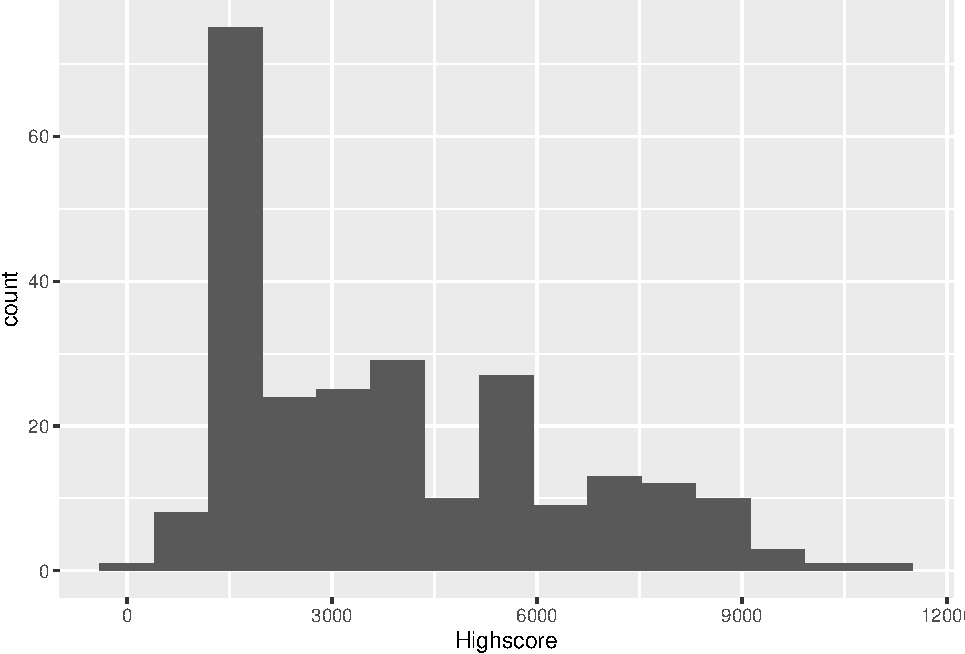
\includegraphics{r_book_files/figure-latex/unnamed-chunk-114-1.pdf}

Es zeigt tatsächlich eine rechtsschiefe Verteilung, die eine deutliche Spitze im unteren Viertel der Bandbreite an Highscores aufweist.

Mit Hilfe eines Boxplots können wir außerdem die Lage der Mittelwerte und die Variation der Highscores in den einzelnen Gruppen überblicksartig beurteilen. Das ist dann schon ein erster Vorgeschmack auf das zu erwartende Ergebnis des folgenden Hypothesentests -- ohne das jedoch geprüft wird, ob die Mittelwerte tatsächlich signifikant von einander abweichen. Zusätzlich lasse ich über \texttt{stat\_summary()}noch die arithmetischen Mittel in schwarz in die Grafik einzeichnen, da der Boxplot lediglich die Mediane darstellt.

\begin{Shaded}
\begin{Highlighting}[]
\NormalTok{df }\SpecialCharTok{\%\textgreater{}\%} 
  \FunctionTok{ggplot}\NormalTok{(}\AttributeTok{mapping =} \FunctionTok{aes}\NormalTok{(}\AttributeTok{x =}\NormalTok{ Schwierigkeitsgrad, }
                       \AttributeTok{y =}\NormalTok{ Highscore, }
                       \AttributeTok{color =}\NormalTok{ Schwierigkeitsgrad)) }\SpecialCharTok{+}
  \FunctionTok{geom\_boxplot}\NormalTok{(}\AttributeTok{width=}\FloatTok{0.5}\NormalTok{) }\SpecialCharTok{+}
  \FunctionTok{stat\_summary}\NormalTok{(}\AttributeTok{fun=}\NormalTok{mean, }\AttributeTok{shape =} \DecValTok{23}\NormalTok{, }\AttributeTok{color =} \StringTok{"black"}\NormalTok{)}
\end{Highlighting}
\end{Shaded}

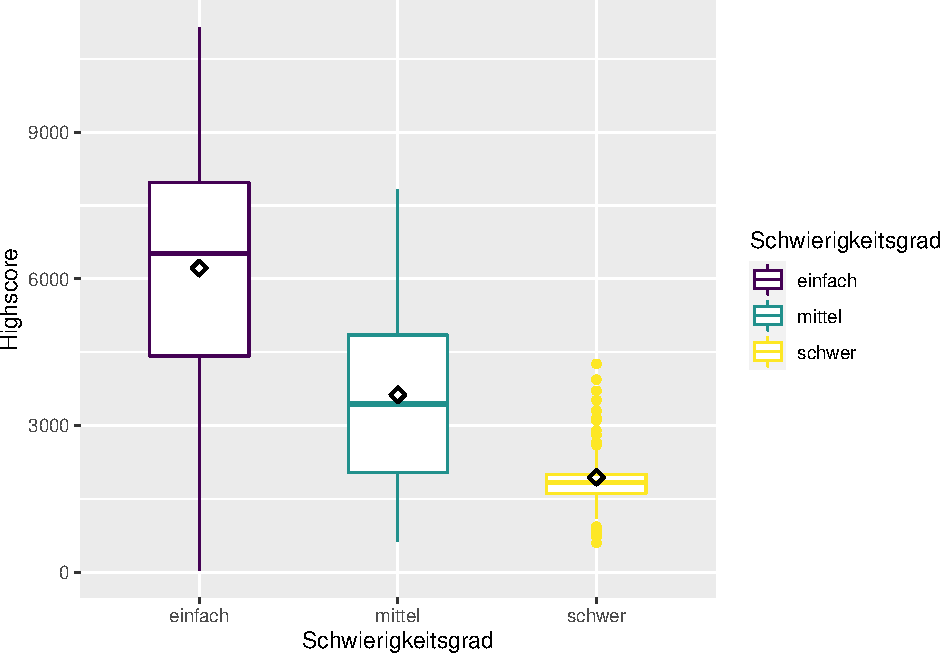
\includegraphics{r_book_files/figure-latex/unnamed-chunk-115-1.pdf}

Tatsächlich, die Mittelwerte in den Gruppen reihen sich genau wie erwartet: Die Personen in der Gruppe ``einfach'' haben den höchsten Highscore erzielt, die in der Gruppe ``schwer'' den niedrigsten. Das ist schon einmal vielversprechend für den Hypothesentest, denn diese Reihung hatten wir ja in der Hypothese prognostiziert. Würde sie hier nicht wie erwartet auftreten, könnten wir den Hypothesentest gleich abbrechen.

Noch etwas wird in dem Boxplot ersichtlich: Die Bandbreite an Highscores ist in der Gruppe ``einfach'' am höchsten: hier liegt sowohl der Minimalwert, als auch der Maximalwert -- und zwar über alle Gruppen hinweg! Das sieht man am der senkrechten violetten Linie, die länger ist, als die Linien der anderen beiden Gruppen. Auch die Quartielgrenzen sind recht weit auseinander (das sieht man an der ``Box''). In dieser Gruppe scheint also die Streuung relativ groß zu sein. In der gelben Gruppe ``schwierig'' ist sie hingegen gering. Das erkannt man an der niedriegen ``Box'' und daran, dass alle Fälle, die außerhalb der Box liegen, noch nicht einmal in Form einer Linie, sondern als Punkte (=Einzelfälle/Ausreißer) dargestellt werden. Die Spieler:innen aus der Gruppe "schwer liegen also viel dichter bei einander als die Spieler:innen der anderen Gruppen.

Der Boxplot prognostiziert folglich eine stark unterschiedliche Varianz oder anders ausgedrückt: \emph{fehlende Varianzhomogenität}. Aus dem letzten Kapitel \protect\hyperlink{anwendungsvoraussetzungen}{T-Test} wissen Sie bereits, dass dies ein Problem sein kann, denn (annähernd) gleiche Varianzen sind eine Anwendungsvoraussetzung, auch für die Varianzanalyse\footnote{Die übrigen Voraussetzungen für die Varianzanalyse sind vom Prinzip her ähnlich zum T-Test. Deshalb wird an dieser Stelle nicht erneut darauf eingegangen}. Hier kommen wieder der \textbf{Levene-Test} und ein korrigierendes Verfahren ins Spiel. Bevor wir also loslegen können mit der eigentlichen Anova schieben wir den Levene-Test ein um sicherzugehen ob die Anwendungsvoraussetzung Varianzhomogenität erfüllt ist oder nicht.

\hypertarget{levene-test}{%
\subsection{Levene-Test}\label{levene-test}}

Der Levene-Test prüft -- wie im letzten Kapitel beschreiben -- ob sich die Varianz in den einzelnen Gruppen unterscheidet (was schlecht wäre) oder nicht (dann wäre die Anwendungsvoraussetzung erfüllt). Bevor wir den Test durchführen, lasse ich mir hier einmal arithmetisches Mittel und die Standardabweichung als standardisiertes Maß der Varianz ausgeben:

\begin{Shaded}
\begin{Highlighting}[]
\NormalTok{df }\SpecialCharTok{\%\textgreater{}\%} 
  \FunctionTok{group\_by}\NormalTok{(Schwierigkeitsgrad) }\SpecialCharTok{\%\textgreater{}\%} 
  \FunctionTok{summarise}\NormalTok{(}\AttributeTok{M =} \FunctionTok{round}\NormalTok{(}\FunctionTok{mean}\NormalTok{(Highscore), }\DecValTok{0}\NormalTok{), }\AttributeTok{SD =} \FunctionTok{round}\NormalTok{(}\FunctionTok{sd}\NormalTok{(Highscore), }\DecValTok{0}\NormalTok{)) }
\end{Highlighting}
\end{Shaded}

\begin{verbatim}
## # A tibble: 3 x 3
##   Schwierigkeitsgrad     M    SD
##   <ord>              <dbl> <dbl>
## 1 einfach             6219  2284
## 2 mittel              3631  1632
## 3 schwer              1946   704
\end{verbatim}

Das sieht tatsächlich nicht so toll aus. Die Standardabweichung ist in der Gruppe ``einfach'' mit SD = 2284 tatsächlich deutlich höher als in der Gruppe ``schwer'' mit SD = \texttt{rdf\ \%\textgreater{}\%\ \ filter(Schwierigkeitsgrad\ ==\ "schwer")\ \%\textgreater{}\%\ summarise(sd(Highscore))\ \%\textgreater{}\%\ round(0)}.

Wir sind vorgewarnt, jetzt wollen wir es genau wissen. Hier kommt der Levene-Test:

\begin{Shaded}
\begin{Highlighting}[]
\NormalTok{df }\SpecialCharTok{\%\textgreater{}\%} 
  \FunctionTok{levene\_test}\NormalTok{(Highscore }\SpecialCharTok{\textasciitilde{}}\NormalTok{ Schwierigkeitsgrad)}
\end{Highlighting}
\end{Shaded}

\begin{verbatim}
## # A tibble: 1 x 4
##     df1   df2 statistic        p
##   <int> <int>     <dbl>    <dbl>
## 1     2   245      42.8 1.17e-16
\end{verbatim}

Wie erwartet zweigt der Levene-Test mit p \textless{} .001 ein signifikantes Ergebnis. Es ist also von Varianzheterogenität auszugehen und wir benötigen eine Korrektur der Prüfgröße F.

\leavevmode\hypertarget{info_levenef}{}%
\textbf{Funfact}

Der Prüfwert des Levene-Tests ist auch ein F-Wert, genau wie der Testwert, der beider Varianzanalyse verwendet wird. Unterschied ist: Bei Levene werden die Varianzen der Gruppen verglichen, bei der Varianzanalyse arithmetische Mittel.

\hypertarget{durchfuxfchrung-der-varianzanalyse}{%
\subsection{Durchführung der Varianzanalyse}\label{durchfuxfchrung-der-varianzanalyse}}

Nun wissen wir schon eine ganze Menge: Wir haben gesehen, dass sich die mittleren Highscores je nach Schwierigkeitsgrad deutlich unterschieden. Und wir wissen, dass wegen der Varianzhomogenität ein korrigierter Test angewendet werden sollte. Als nächstes prüfen wir die Hypothese mit einem Signifikanztest. Erreicht die Profgröße \emph{F} einen gewissen Wert sinkt der p-Wert unter die Grenze von p \textless{} .05 und man würde in dem experimentellen Setting der BA-Arbeit von Herrn Reichelt davon ausgehen, dass der Schwierigkeitsgrad tatsächlich ursächlich für den erzielten Highscore ist (was ja eine völlig plausible Annahme ist).

Die Standard-Funktion aus \texttt{base-R} zur Berechnung von Varianzanalysen ist \texttt{aov()}. Die Funktion kann jedoch keine Korrektur bei Varianzheterogenität vornehmen, weshalb man lieber auf die Funktion \texttt{oneway.test()}, ebenfalls aus base-R zurückgreifen sollte, die dies ermöglicht. Diese Funktion benötigt zwei Argumente. Das dritte hier angegebene Argument ist optional, es sollte dennoch angegeben werden, damit der mögliche Einsatz der Korrektur bewusst und explizit geschieht. Hier die Argumente von \texttt{oneway.test()}:

\begin{enumerate}
\def\labelenumi{\arabic{enumi}.}
\item
  Eine Formel \texttt{formula}, die wie folgt aufgebaut ist: \texttt{abhängige\ Variable\ \textasciitilde{}\ unabhängige\ Variable} (genau wie bei der Regression). Die Tilde \texttt{\textasciitilde{}} bedeutet soviel wie ``wird beeinflusst durch''.
\item
  Ein Datenobjekt \texttt{data} in dem die Variablen und Messwerte zu finden sind, also unser Datensatz.
\item
  Mit dem Argument \texttt{var.equal} lässt sich ein korrigierter Test anfordern. Es steht standardmäßig auf \texttt{FALSE}, so dass nicht von Varianzhomogenität ausgegangen wird und eine s.g. Welch-Korrektur durchgeführt wird. MAn kann es aber auch auf \texttt{TRUE} setzen, wenn der Levene-Test mal auf Varianzhomogenität hinweisen sollte.
\end{enumerate}

Der Output des erzeugten Modells lässt sich mit \texttt{summary()} ausgeben. Mit \texttt{tidy()} aus dem \texttt{broom()}-Paket erhält man allerdings eine hübschere Tabelle:

\begin{Shaded}
\begin{Highlighting}[]
\NormalTok{my\_model }\OtherTok{\textless{}{-}} \FunctionTok{oneway.test}\NormalTok{(}\AttributeTok{formula =}\NormalTok{ Highscore }\SpecialCharTok{\textasciitilde{}}\NormalTok{ Schwierigkeitsgrad, }
                        \AttributeTok{data =}\NormalTok{ df, }
                        \AttributeTok{var.equal =} \ConstantTok{FALSE}\NormalTok{)}

\NormalTok{broom}\SpecialCharTok{::}\FunctionTok{tidy}\NormalTok{(my\_model)}
\end{Highlighting}
\end{Shaded}

\begin{verbatim}
## # A tibble: 1 x 5
##   num.df den.df statistic  p.value method                                       
##    <dbl>  <dbl>     <dbl>    <dbl> <chr>                                        
## 1      2   136.      150. 3.99e-35 One-way analysis of means (not assuming equa~
\end{verbatim}

Ah sehr schön, ausgegeben werden die Freiheitsgrade (df), der F-Wert (statistic) und der zugehörige, sehr kleine p-Wert (p.value). In der letzten Spalte wird noch einmal die verwendete Methode angeführt (One-way Anova) und in Klammern steht auch, dass keine Varianzhomogenität angenommen wurde, wie gewünscht.

\hypertarget{effektstuxe4rke}{%
\subsection{Effektstärke}\label{effektstuxe4rke}}

Als Maß für die Stärke des beobachteten Effekts dient bei der Varianzanalyse \(\eta\)\textsuperscript{2} (Eta-Quadrat). Es berechnet sich aus dem Verhältnis der erklärten Varianz (Quadratsummen zwischen den Gruppen) und der Gesamtvariation. Man kann es mit dem Befehl \texttt{eta\_squared()} aus dem \texttt{effectsize}-Paket ausgeben. Um ein Gesamt-Eta (und kein parteilles) zu erhalten sollte man die Option \texttt{partial} auf \texttt{FALSE} setzen und das Konfidenzintervall auf die für uns üblichen 95\% (Argument \texttt{ci\ =\ 95}):

\begin{Shaded}
\begin{Highlighting}[]
\NormalTok{effectsize}\SpecialCharTok{::}\FunctionTok{eta\_squared}\NormalTok{(my\_model, }
                        \AttributeTok{partial =} \ConstantTok{FALSE}\NormalTok{, }
                        \AttributeTok{ci =} \FloatTok{0.95}\NormalTok{) }
\end{Highlighting}
\end{Shaded}

\begin{verbatim}
## Eta2 |       95% CI
## -------------------
## 0.69 | [0.61, 0.75]
\end{verbatim}

\leavevmode\hypertarget{info_levenef}{}%
\textbf{Achtung, identische Funktionsnamen}

Eine genau gleich benannte Funktion \texttt{eta\_squared()} gibt es auch im Paket \texttt{rstatix}, das ich für den Levene-Test geladen habe. Diese Funktion funktioniert aber nur mit über \texttt{aov()} erzeugten Objekten. Es ist deshalb unter Umständen wichtig explizit zu machen, dass hier die \texttt{eta\_squared()}-Funktion aus dem Paket \texttt{effectsize} verwendet werden soll.

Zusammenfassend lässt sich sagen, dass die bisherigen Ergebnisse für die H1 sprechen: Der F-Wert ist mit p \textless{} .001 signifikant und \(\eta\)\textsuperscript{2} = \text{0,69} steht für einen starken Zusammenhang. Worüber wir jedoch noch keine Aussage machen können ist, ob sich wirklich alle Gruppen jeweils signifikant von einander unterschieden. Dazu werden Posthoc-Test benötigt.

\hypertarget{posthoc-test}{%
\subsection{Posthoc-Test}\label{posthoc-test}}

Der F-Wert repräsentiert die die kombinierte Signifikanz aller Parameter in der Formel. Es ist ein ``Omnibus-Test'': \emph{Alle} Mitelwertunterschiede dürfen ``einsteigen'' und werden gleichzeitig getestet. In unserem Fall sind das drei: (1) der Test zwischen ``einfach'' und ``mittel'', der Test zwischen ``einfach'' und ``schwer'' sowie (3) der Test zwischen ``mittel'' und ``schwer''. Ist der F-Wert signifikant bedeutet das, dass \emph{irgendetwas} in dem getesten Modell signifikant ist. Wir wissen aber nicht genau, ob und welcher der drei Mittelwertvergleiche. Sogenannte \emph{Poshoc-Tests} weisen die Signifikanzen für die einzelnen Mittelwertunterschiede aus.

\leavevmode\hypertarget{info_levenef}{}%
\textbf{Achtung Alphafehler-Kummulation!}

Theoretisch könnte man jetzt einfach hergehen und einen Filter vor die Anova setzen, in dem jeweils eine Gruppe ausgeschlossen wird und nur zwei Gruppen zum Vergleich zugelassen werden. Oder man könnte gleich T-Test mit diesen beiden Gruppen berechnen. Das ist allerdings eine schlechte Idee.

Aus der Inferenzsstatistik-Vorlesung wissen Sie, dass wir bei den hier durchgeführten Nullhypothesentests vorab eine Fehlerwahrscheinlichkeit festlegen, die üblicherweise bei 5 Prozent bzw. bei \(\alpha\) = .05 liegt. Das bedeutet wiederum, das wir in 5 Prozemnt der Fälle eine Fehlentscheidung für ein Signifikantes Ergebnis bewusst einkalkulieren. Das wäre rein statistisch jedes zwanzigste Mal. Gerade wenn viele Signifikanztests durchgeführt werden kann es deshalb vermehrt zu solchen Fehlentscheidungen, den so genannten Alpha-Fehlern kommen. Deshalb muss der kummulierte Alpha-Fehler reduziert werden.

Posthoctests machen genau das: (1) Sie testen sehr viele Mittelwertunterschiede -- nämlich jeweils einzeln die zwischen jeder Gruppe und jeder anderen Gruppe -- und (2) sie korrigieren das Alpha-Fehler-Niveau, so dass es Fehlentscheidungen weniger wahrscheinlich werden und nicht inflationär auftreten. Es gibt viele verschiedene Verfahren für die Alphafehler-Korrektur, die nach ihren jeweiligen Entwicklern benannt sind. Ohne Anspruch auf Vollständigkeit z.B. Bonferoni, Games-Howell, Tamhane und Scheffé. Die Verfahren haben unterschiedliche Anwendungsvoraussetzungen (z.B. Varianzhomogenität) und Vor- und Nachteile. Eine ausführliche Diskussion führt aber an dieser Stelle zu weit.

Selbstverständlich finden sich Posthoc-Tests wieder in unterschiedlichen R-Paketen. Ich mag das \texttt{rstatix}-Paket, weil es pipeable ist und wir es ohnehin schon geladen haben. Darin finden sich verschiedene Funktionen für Posthoc-Tests:

\begin{itemize}
\tightlist
\item
  Falls Varianzhomogenität besteht, kann man die Funktion \texttt{emmeans\_test()} verwenden. ``eenmeans'' steht dabei für ``estimated marginal means''. Die Funktion benötigtdas Datenobjekt als erstes Argument (eine Tidyverse-Konvention), dann die Formel für die Varianzanalyse und schließlich muss man über \texttt{p.adjust.method} die zu verwendende Korrektur angeben, bspw. \texttt{"bonferroni"}
\item
  Der Games-Howell-Test berücksichtigt die Welch-Korrektur und ist über die Funktion \texttt{games\_howell\_test()} nutzbar. Sie benötigt nur das Datenobjekt und die Formel.
\end{itemize}

In unserem Fall brauchen wir natürlich wegen des signifikanten Levene-Tests und der Welch-Korrektur den Games-Howell-Test:

\begin{Shaded}
\begin{Highlighting}[]
\FunctionTok{games\_howell\_test}\NormalTok{(}\AttributeTok{data =}\NormalTok{ df,}
                  \AttributeTok{formula =}\NormalTok{ Highscore }\SpecialCharTok{\textasciitilde{}}\NormalTok{ Schwierigkeitsgrad)}
\end{Highlighting}
\end{Shaded}

\begin{verbatim}
## # A tibble: 3 x 8
##   .y.       group1  group2 estimate conf.low conf.high    p.adj p.adj.signif
## * <chr>     <chr>   <chr>     <dbl>    <dbl>     <dbl>    <dbl> <chr>       
## 1 Highscore einfach mittel   -2588.   -3321.    -1856. 2.03e-13 ****        
## 2 Highscore einfach schwer   -4274.   -4914.    -3633. 4.89e-10 ****        
## 3 Highscore mittel  schwer   -1685.   -2134.    -1236. 8.04e-14 ****
\end{verbatim}

Die Output-Tabelle zeigt drei Zeilen für die drei paarweisen Mittelwertvergleiche. In den beiden ``group''-Spalten steht, welche Gruppen miteinander verglichen werden. Die Spalte ``estimate'' gibt die Differenz zwischen den Gruppenmittelwerten an und dahinter folgen zwei Spalten für das Konfidenzintervall dieser Differenz. Wenn sich die Grenzen der Konfidenzintervalle nicht überschneiden, spricht dies für einen signifikanten Unterschied. Ob eine Mittelwertdifferenz signifikant ist, kann man aber noch leichter in den letzten beiden Spalten sehen. Dort sind der korrigierte p-Wert bzw. das Siginifikanzlevel angegeben.

Das sich die Konfidenzintervalle nicht in ihrem Wertebereich überschneiden lässt sich übrigens auch sehr schön in einem Balkendiagramm mit zusätzlich eingeblendeten Konfidenzintervallgrenzen visuell darstellen. Wir benötigen dazu einen Datensatz, in dem die Mittelwerte, und die Grenzen der Konfidenzintervalle nach Gruppen aufgesplitztet werden. Zur Berechnung der Grenzen des Konfidenzintervalls wird im folgenden Code die Funktion \texttt{mean\_se()} aus dem Paket \texttt{ggplot2} verwendet.

\begin{Shaded}
\begin{Highlighting}[]
\NormalTok{tab\_mean\_ci }\OtherTok{\textless{}{-}}\NormalTok{ df }\SpecialCharTok{\%\textgreater{}\%} 
  \FunctionTok{group\_by}\NormalTok{(Schwierigkeitsgrad) }\SpecialCharTok{\%\textgreater{}\%}
  \FunctionTok{summarise}\NormalTok{(}\FunctionTok{mean\_se}\NormalTok{(Highscore)) }\SpecialCharTok{\%\textgreater{}\%} 
  \FunctionTok{rename}\NormalTok{(}\AttributeTok{Mittelwert =}\NormalTok{ y, }\AttributeTok{CI\_lower =}\NormalTok{ ymin, }\AttributeTok{CI\_higher =}\NormalTok{ ymax) }

\NormalTok{tab\_mean\_ci }
\end{Highlighting}
\end{Shaded}

\begin{verbatim}
## # A tibble: 3 x 4
##   Schwierigkeitsgrad Mittelwert CI_lower CI_higher
##   <ord>                   <dbl>    <dbl>     <dbl>
## 1 einfach                 6219.    5962.     6476.
## 2 mittel                  3631.    3459.     3803.
## 3 schwer                  1946.    1866.     2025.
\end{verbatim}

Aus diesem Datensatz können wir jekt unseren Plot mit zwei Geomen erstellen. Ein Geom für die Balken und eines für die Konfidenzintervalle.

\begin{Shaded}
\begin{Highlighting}[]
\NormalTok{tab\_mean\_ci }\SpecialCharTok{\%\textgreater{}\%}
  \FunctionTok{ggplot}\NormalTok{(}\AttributeTok{mapping =} \FunctionTok{aes}\NormalTok{ (}\AttributeTok{x =}\NormalTok{ Schwierigkeitsgrad, }\AttributeTok{y =}\NormalTok{ Mittelwert)) }\SpecialCharTok{+} 
  \CommentTok{\# Balkendiagramm}
  \FunctionTok{geom\_bar}\NormalTok{(}\AttributeTok{stat=}\StringTok{"identity"}\NormalTok{, }\AttributeTok{fill =} \StringTok{"deeppink"}\NormalTok{, }\AttributeTok{width =} \FloatTok{0.6}\NormalTok{) }\SpecialCharTok{+}
  \CommentTok{\# Konfidenzintervalle}
  \FunctionTok{geom\_errorbar}\NormalTok{(}\AttributeTok{mapping =} \FunctionTok{aes}\NormalTok{(}\AttributeTok{ymin=}\NormalTok{CI\_lower, }\AttributeTok{ymax=}\NormalTok{CI\_higher), }\AttributeTok{width=}\FloatTok{0.4}\NormalTok{)}
\end{Highlighting}
\end{Shaded}

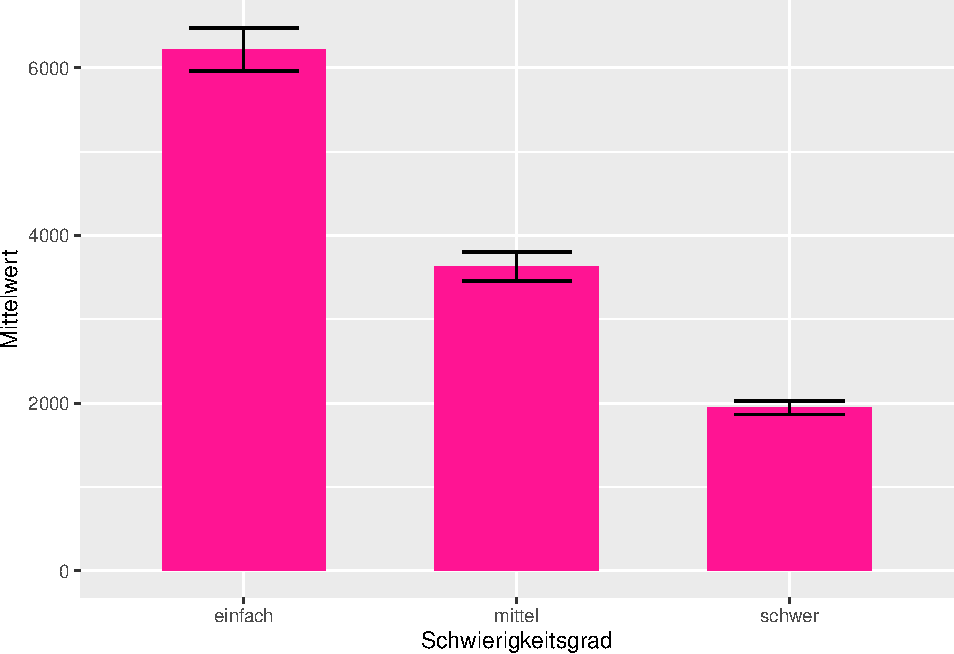
\includegraphics{r_book_files/figure-latex/unnamed-chunk-121-1.pdf}

\hypertarget{ergebnisdarstellung}{%
\subsection{Ergebnisdarstellung}\label{ergebnisdarstellung}}

Selbstverständlich kann man die Ergebnisse einer Varianzanalyse auch in einer Tabelle darstellen. Macht man jedoch nur eine einzelne Analyse, noch dazu wie in diesem Fall ``bloß'' einen Treatment-Check, Ist auch die Darstellung im Text möglich. Für unsere Auswertung sieht dass Ergebnis wie folgt aus:

Die Hypothese wird durch die Varianzanalyse mit Welch-Korrektur gestützt, denn sie zeigt mit \(F_{korrigiert}\) = \text{150} ein höchst signifikantes Ergebnis (p \textless{} .001). Der beobachtete Effekt ist mit \(\eta\)\textsuperscript{2} = \text{0,69} als stark zu bezeichnen. Der Posthc-Test nach Games-Howell zeigt: Alle drei Schwierigkeitsgruppen unterscheiden sich in dem erzielten Highscore von einander. Der Mittelwert des Highscores der Gruppe ``einfach'' ist mit \emph{M} = 6219 (\emph{SD} = 2284) der höchste. Der Mittelwert \emph{M} = 3631 (\emph{SD} = 1632) der Gruppe ``mittel'' ist signifikant geringer, und der Mittelwert der Gruppe ``schwer'' ist mit \emph{M} = 1946 (\emph{SD} = 704) wiederum signifikant geringer als dieser. Wenig überraschend führte also ein höherer Schwierigkeitsgrad dazu, dass die Proband:innen einen geringeren Highscore erzielen.

\hypertarget{zweifaktorielle-varianzanalyse}{%
\section{Zweifaktorielle Varianzanalyse}\label{zweifaktorielle-varianzanalyse}}

Im nächsten Schritt soll eine komplexere Varianzanalyse durchgeführt werden, nämlich eine in der nicht nur ein Einflussfaktor betrachtet wird, sondern gleich zwei. In So einem Modell gibt es drei mögliche Effekte:

\begin{enumerate}
\def\labelenumi{\arabic{enumi}.}
\tightlist
\item
  Einen Haupteffekt von Einflussfaktor A
\item
  Einen Haupteffekt von Einflussfaktor B
\item
  Einen Interaktionseffekt der beiden Einflussfakoren
\end{enumerate}

\leavevmode\hypertarget{info_interactionanova}{}%
\textbf{Haupt- \& Interaktionseffekte}

\emph{Haupteffekt} bedeutet, dass ein Faktor direkt unt unter allen (einbezogenen) Bedingungen auf die abhängige Variable wirkt.

Bei \emph{Interaktionseffekten} wirken zwei (oder mehr) Faktoren in komplexer Weise zusammen. Der Effekt geht über eine reine Addition der Haupteffekte der beiden Einflussvariablen hinaus. Bei einer Interaktion ist die Wirkung eines Faktors abhängig von den Ausprägungen des anderen Faktors. Das heißt zum Beispiel, dass sich die Wirkung bei gleichzeitigem Auftreten besonders verstärken kann. Es sind aber auch Abschwächungseffekte denkbar, oder dass eine bestimmte Wirkung von Faktor A nur auftritt, wenn auch Faktor B zu einem gewissen Grad gegeben ist. -- Der \emph{F}-Wert verändert sich.

Interaktionseffekte zu untersuchen ist natürlich besonders spannend.

Wir greifen in diesem Beispiel wieder auf die Daten von Carsten Reichelt zurück und nehmen nun einen zusätzlichen Einflussfaktor hinzu, nämlich die Wettkampfpräferenz. Dieses Konstrukt drückt aus, inwiefern ein:e Spieler:in bereit ist, sich einem Wettkampf zu stellen. Die Variable ist nominal/dichotom umd hat zwei Ausprägungen: geringe und hohe Wettkampfpräferenz.

\begin{Shaded}
\begin{Highlighting}[]
\NormalTok{df }\SpecialCharTok{\%\textgreater{}\%} 
\NormalTok{  janitor}\SpecialCharTok{::}\FunctionTok{tabyl}\NormalTok{(Wettkampfpraeferenz) }\SpecialCharTok{\%\textgreater{}\%} 
  \FunctionTok{adorn\_rounding}\NormalTok{(}\DecValTok{2}\NormalTok{) }\SpecialCharTok{\%\textgreater{}\%} 
  \FunctionTok{adorn\_totals}\NormalTok{() }
\end{Highlighting}
\end{Shaded}

\begin{verbatim}
##         Wettkampfpraeferenz   n percent
##  geringe Wettkampfpräferenz 131    0,53
##     hohe Wettkampfpräferenz 117    0,47
##                       Total 248    1,00
\end{verbatim}

Für unser Hypothesenkonstrukt bedeutet das, dass wir nun drei Hypothesen haben:

\emph{H1: Der Schwierigkeitsgrad beeinflusst den Highscore negativ (siehe oben).}

\emph{H2: Die Wettkampfpräferenz beeinflusst den Highscore positiv.}

\emph{H3: Es gibt einen Interaktionseffekt zwischen Schwierigkeitsgrad und Wettkampfpräferenz.}

Für H3 sollten wir natürlich auch überlegen, welcher Art die Interaktion sein könnte. Ich lehne mich jetzt mal aus dem Fenster und prognostiziere, dass man erwarten könnte, dass der Einfluss von Wettkampfpräferenz mit steigendem Schwierigkeitsgrad abnimmt. Meine Begründung dafür wäre, das man bei einem hohen Schwierigkeitsgrad weniger Einfluss auf den Highscore hat, selbst wenn man eine hohe Wettkampfpräferenz hat. Das Ergebnis des Highscores ist schließlich auch noch von vielen anderen Punkten abhängig, wie z.B. Spielerfahrung oder generelle Reaktionsgeschwindigkeit. Meine präzisierte H3 lautet also:

\emph{H3: Bei zunehmendem Schwierigkeitsgrad nimmt der Einfluss der Wettkampfpräferenz ab.}

\leavevmode\hypertarget{info_interactionanova}{}%
\textbf{Muss H1 noch einmal geprüft werden? Ja!}
Man könnte ja denken, dass man H1 auch weglassen könnte, schließlich haben wir sie im vorigen Abschnitt bereits geprüft. Allerdings kann es natürlich sein, dass sich der gefundene Effekt bei der Hinzunahme neuer Einflussfaktoren verändert, z.B. geringer ausfällt (der \emph{F}-Wert würde in diesem Fall geringer und damit auch die Signifikanz).

Außerdem können wir die Effekte beider Einflussfaktoren miteinander vergleichen, wenn wir beide aufnehmen.

\hypertarget{deskriptive-analyse-1}{%
\subsection{Deskriptive Analyse}\label{deskriptive-analyse-1}}

Wie immer: Vor dem Signifikanztest wird deskriptiv ausgewertet. Es muss festgestellt werden, ob die Mittelwerte in die Prognostizierte Richtung weisen. Für H1 und den Schwierigkeitsgrad haben wir dies im letzten Abschnitt bereits bestätigt.

Aber auch für den zweiten Haupteffekt und die Wettkampfpräferenz (H2) sieht es gut aus, denn tatsächlich ist der Highscore der PRobanden hhöher, wenn die Wettkampfpräferenz höher ist.

\begin{Shaded}
\begin{Highlighting}[]
\NormalTok{df }\SpecialCharTok{\%\textgreater{}\%} 
  \FunctionTok{group\_by}\NormalTok{(Wettkampfpraeferenz) }\SpecialCharTok{\%\textgreater{}\%} 
  \FunctionTok{summarize}\NormalTok{(}\AttributeTok{n =} \FunctionTok{n}\NormalTok{(), }
            \AttributeTok{M =} \FunctionTok{round}\NormalTok{(}\FunctionTok{mean}\NormalTok{(Highscore)),}
            \AttributeTok{SD =} \FunctionTok{round}\NormalTok{(}\FunctionTok{sd}\NormalTok{(Highscore)))}
\end{Highlighting}
\end{Shaded}

\begin{verbatim}
## # A tibble: 2 x 4
##   Wettkampfpraeferenz            n     M    SD
##   <ord>                      <int> <dbl> <dbl>
## 1 geringe Wettkampfpräferenz   131  3550  2080
## 2 hohe Wettkampfpräferenz      117  4331  2652
\end{verbatim}

Nun zum Interaktionseffekt. Um die Werte zu veranschaulichen Gruppieren wir nicht nur nach einer unabhängigen Variable sondern nach beiden. Weil wir diese Tabelle später noch einmal benötigen, wird sie als objekt \texttt{desc\_table} abgespeichert.

\begin{Shaded}
\begin{Highlighting}[]
\NormalTok{desc\_table }\OtherTok{\textless{}{-}}\NormalTok{ df }\SpecialCharTok{\%\textgreater{}\%} 
  \FunctionTok{group\_by}\NormalTok{(Schwierigkeitsgrad, Wettkampfpraeferenz) }\SpecialCharTok{\%\textgreater{}\%} 
  \FunctionTok{summarize}\NormalTok{(}\AttributeTok{n =} \FunctionTok{n}\NormalTok{(), }
            \AttributeTok{M =} \FunctionTok{round}\NormalTok{(}\FunctionTok{mean}\NormalTok{(Highscore)),}
            \AttributeTok{SD =} \FunctionTok{round}\NormalTok{(}\FunctionTok{sd}\NormalTok{(Highscore)))}

\NormalTok{desc\_table }
\end{Highlighting}
\end{Shaded}

\begin{verbatim}
## # A tibble: 6 x 5
## # Groups:   Schwierigkeitsgrad [3]
##   Schwierigkeitsgrad Wettkampfpraeferenz            n     M    SD
##   <ord>              <ord>                      <int> <dbl> <dbl>
## 1 einfach            geringe Wettkampfpräferenz    37  5267  2196
## 2 einfach            hohe Wettkampfpräferenz       42  7058  2037
## 3 mittel             geringe Wettkampfpräferenz    50  3768  1660
## 4 mittel             hohe Wettkampfpräferenz       40  3458  1601
## 5 schwer             geringe Wettkampfpräferenz    44  1858   617
## 6 schwer             hohe Wettkampfpräferenz       35  2056   796
\end{verbatim}

Diese Tabelle ist etwas unübersichtlich. Aber eigentlich ist es auch nicht so schlimm, wenn man weiß, wonach man suchen muss. Es ist hier relevant zu schauen, ob sich die Mittelwerte in zusammengehörigen Zeilen unterschieden, z.B. also die beiden Zeilen ``Schwierigkeitsgrad leicht''. Tatsöchlich ist in diesen beiden Zeilen ein deutlciher Mittelwertunterschied zu finden. Bei ``mittel'' und ``schwer'' ist hingegen kaum eine Deifferenz.

An den Werten für n können wir sehen, dass es auch für jede Kombination der beiden Einflussfaktoren im Datensatz eine beruhigend hohe Anzahl an n \textgreater{} 30 Fällen gibt. Wir können deshalb nach dem zentralen Grenzwerttheorem davon ausgehen, dass sich Stichprobenmittelwerte unterschiedlicher Stichproben normal verteilen würden, selbst in den jetzt sechs Untergruppen.

Zur visuellen Analyse lässt sich der Boxplot über die ggplot-Funktion \texttt{facet\_wrap} leicht so aufsplitten, dass alle sechs Gruppen sichtbar werden:

\begin{Shaded}
\begin{Highlighting}[]
\NormalTok{df }\SpecialCharTok{\%\textgreater{}\%} 
  \FunctionTok{ggplot}\NormalTok{(}\AttributeTok{mapping =} \FunctionTok{aes}\NormalTok{(}\AttributeTok{x =}\NormalTok{ Schwierigkeitsgrad, }\AttributeTok{y =}\NormalTok{ Highscore, }\AttributeTok{color =}\NormalTok{ Schwierigkeitsgrad)) }\SpecialCharTok{+}
  \FunctionTok{geom\_boxplot}\NormalTok{(}\AttributeTok{width=}\FloatTok{0.5}\NormalTok{) }\SpecialCharTok{+}
  \FunctionTok{stat\_summary}\NormalTok{(}\AttributeTok{fun=}\NormalTok{mean, }\AttributeTok{shape =} \DecValTok{23}\NormalTok{, }\AttributeTok{color =} \StringTok{"black"}\NormalTok{) }\SpecialCharTok{+}
  \FunctionTok{facet\_wrap}\NormalTok{(}\FunctionTok{vars}\NormalTok{(Wettkampfpraeferenz))}
\end{Highlighting}
\end{Shaded}

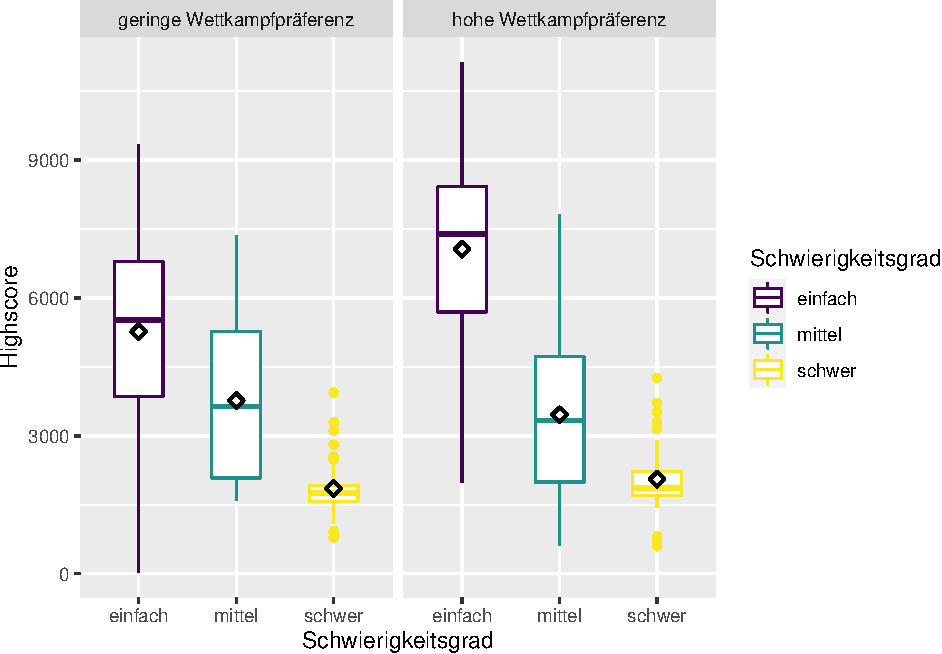
\includegraphics{r_book_files/figure-latex/unnamed-chunk-125-1.pdf}

Augenscheinlich hat sich die Lage durch die Aufteilung in nun sechs Gruppen nicht wesentlich verschlimmert, denn die jeweils gleichfarbigen Box-Plots weisen immer die höchste Ähnlichkeit zueinander auf und sind von den andersfarbigen immer deutlich verschieden.

\hypertarget{levene-test-1}{%
\subsection{Levene-Test}\label{levene-test-1}}

Wir wissen bereits aus dem vorigen Abschnitt, dass wir es hinsichtlich der Gruppenvariable Schwierigkeit mit heterogenen Varianzen bei der Variable Highscore zu tun haben. Außerdem existiert für die Mehrfaktorielle Varianzanalyse leider keine WElch-Korrektur. Der Vollständigkeit halber, wird hier dennoch demonstriert, wie eine Analyse der unterschiedlichen Streuung bei einer Zweifaktoriellen Varianzanalyse aussieht.

Zuerst der Levene-Test für den Einflussfaktor Wettkampfpräferenz:

\begin{Shaded}
\begin{Highlighting}[]
\NormalTok{df }\SpecialCharTok{\%\textgreater{}\%} 
  \FunctionTok{levene\_test}\NormalTok{(Highscore }\SpecialCharTok{\textasciitilde{}}\NormalTok{ Wettkampfpraeferenz)}
\end{Highlighting}
\end{Shaded}

\begin{verbatim}
## # A tibble: 1 x 4
##     df1   df2 statistic       p
##   <int> <int>     <dbl>   <dbl>
## 1     1   246      8.03 0.00499
\end{verbatim}

Ergebnis: Ebenfalls signifikant, also ungleiche Varianzen.

Und da wir uns in H3 auch für den Interaktionseffekt interessieren folgt noch ein multifaktorieller Levene-Test. Die Interaktion wird eingebracht über den Operator \texttt{*} in der Formel.

\begin{Shaded}
\begin{Highlighting}[]
\NormalTok{df }\SpecialCharTok{\%\textgreater{}\%} 
  \FunctionTok{levene\_test}\NormalTok{(Highscore }\SpecialCharTok{\textasciitilde{}}\NormalTok{ Schwierigkeitsgrad }\SpecialCharTok{*}\NormalTok{ Wettkampfpraeferenz)}
\end{Highlighting}
\end{Shaded}

\begin{verbatim}
## # A tibble: 1 x 4
##     df1   df2 statistic        p
##   <int> <int>     <dbl>    <dbl>
## 1     5   242      13.2 2.33e-11
\end{verbatim}

Wie zu erwarten, ein drittes signifikantes Ergebnis. Wir können also auf keinen Fall von Varianzhomogenität ausgehen. Dieses Wissen bleibt insofern ohne Konsequenzen, als dass wir hier eine ganz normale zweifaktorielle Varianzanalyse berechnen werden, weil die Welch-Korrektur für dieses Verfahren fehlt. Wir behalten aber im Hinterkopf, dass das Ergebnis der nun folgenden Analyse möglicherweise verzerrt ist, weil die Anwendungsvoraussetzung der Varianzhomogenität verletzt wird.

\hypertarget{durchfuxfchrung-einer-mehrfaktoriellen-varianzanalyse}{%
\subsection{Durchführung einer mehrfaktoriellen Varianzanalyse}\label{durchfuxfchrung-einer-mehrfaktoriellen-varianzanalyse}}

Nun folgt der Signifikanztest, bzw. die Signifikanztests, es sind ja mehrere und zwar gleichzeitig. Es gibt -- wie so oft -- viele Pakete mit denen man eine zweifaktorielle Varianzanalyse berechnen könnte, z.B. auch das Paket \texttt{rstatix}, das wir ja bereits geladen haben. Ich habe mich hier jedoch für das \texttt{afex}-Paket entschieden. Es ist ein spezielles Paket zur Berechnung von Anovas mit Experimentaldaten und bietet dabei viele Möglichkeiten. -- Auch wenn ihre Analysen komplexer werden und über das hier gezeigte hinausgehen, können Sie bei dem Paket bleiben.

Bevor es losgeht, eine Anmerkung vorab: Es gibt bei der mehrfaktoriellen Varianzanalyse unterschiedliche ``Typen''. Sie unterscheiden sich darin, wie die Abweichungen der individuellen Messungen vom Gesamtmittelwert den einzenen Faktoren zugeschlagen werden. Dieses Thema kann hier nicht vertieft werden. Wichtig ist aber, dass wir für die unsere Berechnung die Quadratsummenzerlegung \emph{Typ III} benötigen, dies bietet das base-Paket nicht.

\begin{verbatim}
## Coefficient covariances computed by hccm()
\end{verbatim}

\begin{verbatim}
## ANOVA Table (type III tests)
## 
##                                   Effect DFn DFd     F       p p<.05   ges
## 1                     Schwierigkeitsgrad   2 242 138,3 9,0e-41     * 0,533
## 2                    Wettkampfpraeferenz   1 242   7,5 7,0e-03     * 0,030
## 3 Schwierigkeitsgrad:Wettkampfpraeferenz   2 242   9,6 9,4e-05     * 0,074
\end{verbatim}

Die Funktion \texttt{aov\_car} aus dem \texttt{afex}-Paket benötigt eine Formel der Form \texttt{abhängige\ Variable\ \textasciitilde{}\ unabhängige\ Variable}, genau wie beim Levene-Test. Es gibt aber noch eine Besonderheit: Angegeben werden muss außerdem noch ein ``Fehlerterm''. Der Fehlerterm stellt in dem Modell die nicht erklärte Varianz dar, die jeder Messpunkt aufweist. Es ist wichtig, dass hier eine Variable eingesetzt wird, die für jeden Fall im Datensatz einen \emph{eineindeutigen} Wert hat (= kein Wert darf doppelt vorkommen). Hier bietet sich die ``laufende Nummer'', also die Variable \texttt{lfdn} an.

\begin{Shaded}
\begin{Highlighting}[]
\NormalTok{my\_model }\OtherTok{\textless{}{-}}\NormalTok{ afex}\SpecialCharTok{::}\FunctionTok{aov\_car}\NormalTok{(Highscore }\SpecialCharTok{\textasciitilde{}}\NormalTok{ Schwierigkeitsgrad }\SpecialCharTok{+}\NormalTok{ Wettkampfpraeferenz }\SpecialCharTok{+} 
\NormalTok{                                      Schwierigkeitsgrad }\SpecialCharTok{*}\NormalTok{ Wettkampfpraeferenz }\SpecialCharTok{+}
                                      \FunctionTok{Error}\NormalTok{(lfdn), }
                          \AttributeTok{data =}\NormalTok{ df)}
\end{Highlighting}
\end{Shaded}

\begin{verbatim}
## Contrasts set to contr.sum for the following variables: Schwierigkeitsgrad, Wettkampfpraeferenz
\end{verbatim}

\begin{Shaded}
\begin{Highlighting}[]
\NormalTok{my\_model}
\end{Highlighting}
\end{Shaded}

\begin{verbatim}
## Anova Table (Type 3 tests)
## 
## Response: Highscore
##                                   Effect     df        MSE          F  ges
## 1                     Schwierigkeitsgrad 2, 242 2547712,45 138,25 *** ,533
## 2                    Wettkampfpraeferenz 1, 242 2547712,45    7,52 ** ,030
## 3 Schwierigkeitsgrad:Wettkampfpraeferenz 2, 242 2547712,45   9,64 *** ,074
##   p.value
## 1   <.001
## 2    ,007
## 3   <.001
## ---
## Signif. codes:  0 '***' 0,001 '**' 0,01 '*' 0,05 '+' 0,1 ' ' 1
\end{verbatim}

Sehr schön, alle \emph{F}-Werte sind signifikant! Das spricht für die Hypothesen. Weil die deskriptive Analyse der Haupteffekte auch in die richtige Richtung zeigte, können H1 und H2 jetzt schon als durch die Daten bestätigt angesehen werden. Bei H3, der Inetraktionshypothese ist es nicht ganz so klar, aber irgendwas signifikantes scheint es auch hier zu geben, zum Verständnis hilft ein Interaktionsplot.

Zuvor berechnen wir aber noch schnell die Effektstärken des Modells, das nicht-partielle \(_eta^2^\):

\begin{Shaded}
\begin{Highlighting}[]
\FunctionTok{eta\_squared}\NormalTok{(my\_model, }\AttributeTok{partial =} \ConstantTok{FALSE}\NormalTok{, }\AttributeTok{ci =} \FloatTok{0.95}\NormalTok{)}
\end{Highlighting}
\end{Shaded}

\begin{verbatim}
## Type 3 ANOVAs only give sensible and informative results when covariates are
##   mean-centered and factors are coded with orthogonal contrasts (such as those
##   produced by 'contr.sum', 'contr.poly', or 'contr.helmert', but *not* by the
##   default 'contr.treatment').
\end{verbatim}

\begin{verbatim}
## # Effect Size for ANOVA (Type III)
## 
## Parameter                              | Eta2 |       95% CI
## ------------------------------------------------------------
## Schwierigkeitsgrad                     | 0.51 | [0.42, 0.58]
## Wettkampfpraeferenz                    | 0.01 | [0.00, 0.06]
## Schwierigkeitsgrad:Wettkampfpraeferenz | 0.04 | [0.00, 0.09]
\end{verbatim}

Eindeutig die größte Effektstärke zeigt der Haupteffekt des Schwierigkeitsgrades (H1). -- Gegenüber dem Test mit der einfaktoriellen Varianzanalyse fällt es jedoch geringfügig kleiner aus. Die anderen beiden Effekte sind irgendwie existent, aber vergleichsweise gering.

\hypertarget{visualisierung}{%
\subsection{Visualisierung}\label{visualisierung}}

Die Visualisierung von Interaktionseffekten hilft erheblich bei der Interpretation. Am einfachsten ist, es, wenn wir als Basis für die Visualisierung die Tabelle benutzen, die wir im Abschnitt \protect\hyperlink{deskriptive-analyse-1}{Deskriptive Analyse} erzeugt hatten. Wir brauchen aus dieser Tabelle die beiden Einflussvariablen und die Mittelwerte:

\begin{Shaded}
\begin{Highlighting}[]
\NormalTok{desc\_table }\SpecialCharTok{\%\textgreater{}\%} 
  \FunctionTok{select}\NormalTok{(Schwierigkeitsgrad, Wettkampfpraeferenz, M)}
\end{Highlighting}
\end{Shaded}

\begin{verbatim}
## # A tibble: 6 x 3
## # Groups:   Schwierigkeitsgrad [3]
##   Schwierigkeitsgrad Wettkampfpraeferenz            M
##   <ord>              <ord>                      <dbl>
## 1 einfach            geringe Wettkampfpräferenz  5267
## 2 einfach            hohe Wettkampfpräferenz     7058
## 3 mittel             geringe Wettkampfpräferenz  3768
## 4 mittel             hohe Wettkampfpräferenz     3458
## 5 schwer             geringe Wettkampfpräferenz  1858
## 6 schwer             hohe Wettkampfpräferenz     2056
\end{verbatim}

Was im Interaktionsdiagramm dargestellt werden soll, ist genau das, was oben in der Tabelle steht: Die Mittelwerte des Highscores und zwar in Abhängigkeit von den beiden unabhängigen Variablen. Hätten wir nur einen Einflussfaktor, würden wir das mit einem Balkendiagramm machen (siehe oben: Schwierigkeitsgrad auf die x-Achse, Mittelwert des Highscores auf die y-Achse).

Bei zwei Faktoren bietet sich ein Liniendiagramm an. Der zweite Faktor kann dann durch unterschiedliche Linien (Argument \texttt{group}) dargestellt werden, die zur besseren Übersichtlichkeit auch noch verschieden eingefärbt werden können (Argument \texttt{color}).

\begin{Shaded}
\begin{Highlighting}[]
\NormalTok{desc\_table }\SpecialCharTok{\%\textgreater{}\%} 
  \FunctionTok{ggplot}\NormalTok{(}\AttributeTok{mapping =} \FunctionTok{aes}\NormalTok{(}\AttributeTok{x =}\NormalTok{ Schwierigkeitsgrad, }\AttributeTok{y =}\NormalTok{ M, }
                       \AttributeTok{group =}\NormalTok{ Wettkampfpraeferenz, }\AttributeTok{color =}\NormalTok{ Wettkampfpraeferenz)) }\SpecialCharTok{+}       
  \FunctionTok{geom\_line}\NormalTok{() }\SpecialCharTok{+} 
  \CommentTok{\# Ab hier nur noch "Aufhübschung" des Plots}
  \FunctionTok{ylim}\NormalTok{(}\DecValTok{0}\NormalTok{, }\DecValTok{8000}\NormalTok{) }\SpecialCharTok{+}
  \FunctionTok{labs}\NormalTok{(}\AttributeTok{x =} \StringTok{"Schwierigkeitsgrad"}\NormalTok{, }
       \AttributeTok{y =} \StringTok{"Mittelwert Highscore"}\NormalTok{) }\SpecialCharTok{+} 
  \FunctionTok{theme\_minimal}\NormalTok{() }\SpecialCharTok{+}
  \FunctionTok{scale\_color\_manual}\NormalTok{(}\AttributeTok{values =} \FunctionTok{c}\NormalTok{(}\StringTok{"green"}\NormalTok{, }\StringTok{"deeppink"}\NormalTok{))}
\end{Highlighting}
\end{Shaded}

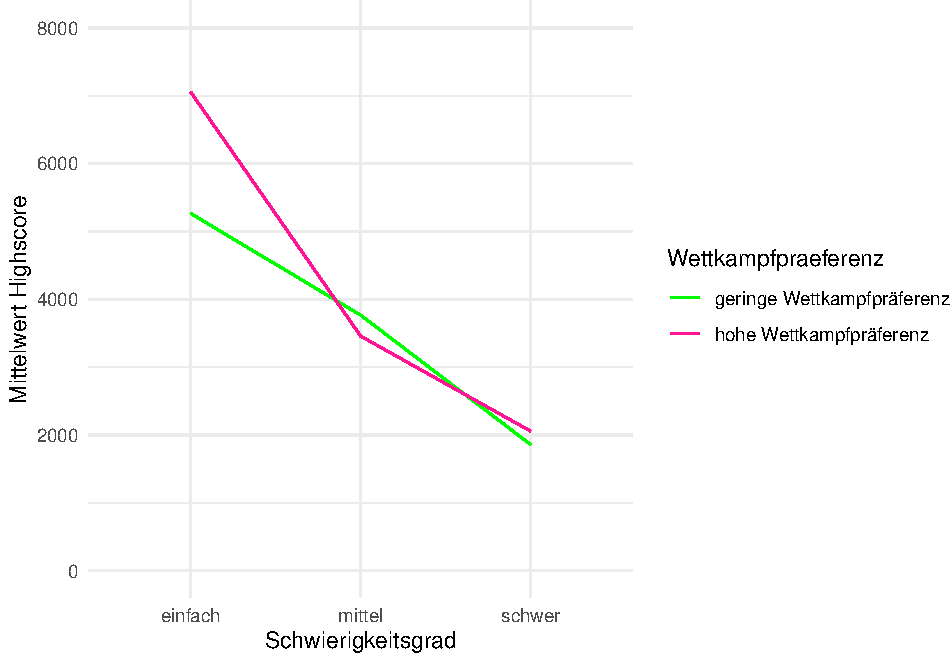
\includegraphics{r_book_files/figure-latex/unnamed-chunk-132-1.pdf}

In dem Interaktionsdiagramm zeigt sich, dass die von mir Prognostizierte Interaktion vor allem im einfachen Schwierigkeitsgrad zum Tragen kommt. Hier ist es tatsächlich so, dass Probandinnen mit hoher Wettkampfpräferenz deutlich besser abschneiden als solche mit niedriger. Auf mittlerem Schwierigkeitsgrad ist die Tendenz jedoch umgedreht. Hier sind Personen mit niedriger Wettkampfpräferenz etwas besser. Der Mittelwertunterschied ist jedoch gering. Bei schweren Schwirigkeitsgrad dreht es sich wieder, aber auch hier ist die Mittelwertdifferenz gering. Es ist also kompliziert. Möglicherweise gibt es einen zusätzlichen Effekt, bei dem Personen mit hoher Wettkampfpräferenz durch einen besonders schweren Schwierigkeitsgrad zusätzlich angespornt werden einen hohen Highscore zu erzielen. Um das zu untersuchen sind unsere Daten aber leider nicht differenziert genug. Festzuhalten ist aber, dass sich die H3 (A-Version) bestätigen lässt (das zeigt der \emph{F}-Wert oben) und dass zumindest die visuellen Ergebnisse für Gruppe ``leicht'' für die präzisierte B-Version der H3 sprechen.

Es stellt sich jetzt natürlich die Frage, welche der beobachteten Mittelwertunterschiede sind signifikant?

\hypertarget{posthoc-tests}{%
\subsection{Posthoc-Tests}\label{posthoc-tests}}

Bis hierhin haben wir festgestellt, dass sich wohl alle drei Hypothesen bestätigen lassen. Müssen wir einen erneuten Posthoc-Test durchführen? Und wenn ja für welche Hypothesen?

Für H1 (Haupteffekt des Schwierigkeitsgrades) haben wir den Post-Hoc-Test bereits im Ersten Abschnitt bei der einfaktoriellen Varianzanalyse ausgefüht.

Für H2 (Haupteffekt der Wettkampfpräferenz) brauchen wir keinen Posthoc-Test, denn der Faktor Wettkampfpräferenz hat nur zwei Ausprägungen. Die Varianzanalyse hat einen signifikanten Haupterfeffekt ergeben, es ist klar das sich nur diese beiden unterschieden können (um beim Bild des Omnibustests zu bleiben: Es sitzt nur ein Mittelwertunterschied im Bus)

Für H3 (Interaktion) wäre ein Posthoc-Test natürlich interessant. Es wäre wichtig zu wissen, ob sich die Personen mit hoher vs.~niedriger Wettkampfpräferenz in der Gruppe leichter Schwierigkeitsgrad tatsächlich signifikant unterscheiden. Und natürlich auch, ob in den anderen Schwierigkeitsgraden signifikante Unterschiede vorliegen.

Ich habe leider noch keine eleganze Version gefunden, mit der man in R einen Posthoc-Test für Interaktionseffekte rechnen kann -- für Hinweise wäre ich dankbar. Bis ich diesen Hinweis erhalten habe, behelfe ich mich damit, dass ich aus den beiden Faktoren einen neue, kombinierte Gruppenvariable bilde und diese dann in den Posthoctest gebe.

Der folgende Code ist advanced, der Vollständigkeit halber zeige ich ihn hier dennoch:

\begin{Shaded}
\begin{Highlighting}[]
\NormalTok{df }\SpecialCharTok{\%\textgreater{}\%} 
  \FunctionTok{mutate}\NormalTok{(}\AttributeTok{Gruppe =} \FunctionTok{str\_c}\NormalTok{(Schwierigkeitsgrad, Wettkampfpraeferenz, }\AttributeTok{sep =} \StringTok{"{-}"}\NormalTok{)) }\SpecialCharTok{\%\textgreater{}\%} 
  \FunctionTok{games\_howell\_test}\NormalTok{(}\AttributeTok{formula =}\NormalTok{ Highscore }\SpecialCharTok{\textasciitilde{}}\NormalTok{ Gruppe) }\SpecialCharTok{\%\textgreater{}\%} 
  \CommentTok{\# Zur Übersichtlichkeit Zahlenwerte runden}
  \FunctionTok{mutate\_at}\NormalTok{(}\FunctionTok{c}\NormalTok{(}\StringTok{"estimate"}\NormalTok{, }\StringTok{"conf.low"}\NormalTok{, }\StringTok{"conf.high"}\NormalTok{), format, }\AttributeTok{digits =} \DecValTok{0}\NormalTok{, }\AttributeTok{nsmall =} \DecValTok{0}\NormalTok{) }\SpecialCharTok{\%\textgreater{}\%} 
  \CommentTok{\# Zur Übersichtlichkeit nur relevante Variablen auswählen}
  \FunctionTok{select}\NormalTok{(group1, group2, estimate, p.adj.signif) }\SpecialCharTok{\%\textgreater{}\%} 
  \CommentTok{\# Nur die Mittelwertunterschiede herausfiltern die mich tatsächlich interessieren }
  \FunctionTok{filter}\NormalTok{(}\FunctionTok{str\_extract}\NormalTok{(group1, }\StringTok{"\^{}[einfach|mittel|schwer]"}\NormalTok{) }\SpecialCharTok{==} \FunctionTok{str\_extract}\NormalTok{(group2, }\StringTok{"\^{}[einfach|mittel|schwer]"}\NormalTok{))}
\end{Highlighting}
\end{Shaded}

\begin{verbatim}
## # A tibble: 3 x 4
##   group1                        group2                     estimate p.adj.signif
##   <chr>                         <chr>                      <chr>    <chr>       
## 1 einfach-geringe Wettkampfprä~ einfach-hohe Wettkampfprä~ " 1791"  **          
## 2 mittel-geringe Wettkampfpräf~ mittel-hohe Wettkampfpräf~ " -310"  ns          
## 3 schwer-geringe Wettkampfpräf~ schwer-hohe Wettkampfpräf~ "  198"  ns
\end{verbatim}

Ich interessiere mich vor allem für die Mittelwertunterschiede innerhalb jedes jedes Schwierigkeitsgerades. Deshalb habe ich durch einen Filter, der mit ``Regular Expressions'' arbeitet hier nur die herausgefiltert. Schaut man sich die Signifikanzniveaus drei Mittelwertunterschiede an, bestätigt sich, was auch schon anhand der Interaktionsgrafik zu vermuten war: Ein Signifikanter Mittelwertunterschied der Wettkampfpräferenz besteht lediglich in der Gruppe ``leichter Schwierigkeitsgrad''.

\hypertarget{abschlieuxdfende-beurteilung-des-hypothesentests}{%
\subsection{Abschließende Beurteilung des Hypothesentests}\label{abschlieuxdfende-beurteilung-des-hypothesentests}}

Alle drei Hypothesn ließen sich mit den Daten bestätigen. Jedoch ist der Haupteffekt des Schwierigkeitsgerades deutlich am größten, während der Haupteffekt der Wettkampfpräferenz gering ausfällt. Es gibt jedoch eine interessante Interaktion zwischen beiden Faktoren, die jedoch lediglich im leichten Schwierigkeitsgrad zum Tragen kommt: Dieser Schwierigkeitsgrad ermöglicht es offenbar den Proband:innen mit einer hohen Wettkampfpräferenz deutlich vor denen, die nur eine niedrig ausgeprägte Wettkampfpräferenz haben, hervorzustechen und einen signifikant höheren Highscore zu erzielen. In schwereren Schwierigkeitsgraden niveliert sich der Einfluss der Wettkampfpräferenz.

  \bibliography{literature.bib}

\end{document}
